\documentclass[ALICE,manyauthors]{ALICE_analysis_notes}
%\documentclass[ALICE,manyauthors]{ALICE_scientific_notes}
%

\usepackage{natbib}
\usepackage[toc,page]{appendix}

\newcommand{\pt}{\ensuremath{p_{\mathrm{T}}}}
\newcommand{\ptreco}{\ensuremath{p_{\mathrm{T}}^{\mathrm{reco}}}}
\newcommand{\pttruth}{\ensuremath{p_{\mathrm{T}}^{\mathrm{true}}}}
\newcommand{\pttrack}{\ensuremath{p_{\mathrm{T}}^{\mathrm{track}}}}
\newcommand{\ptgamma}{\ensuremath{p_{\mathrm{T}}^{\mathrm{\gammaiso}}}}
\newcommand{\ptcluster}{\ensuremath{p_{\mathrm{T}}^{\mathrm{cluster}}}}


\newcommand{\Ntrig}{\ensuremath{N_{\mathrm{trig}}}}
\newcommand{\Nsame}{\ensuremath{N_{\mathrm{same}}}}
\newcommand{\Nmixed}{\ensuremath{N_{\mathrm{mixed}}}}


\newcommand{\CBR}{\ensuremath{C_{\mathrm{BR}}}}
\newcommand{\CSR}{\ensuremath{C_{\mathrm{SR}}}}
\newcommand{\TBR}{\ensuremath{T_{\mathrm{BR}}}}
\newcommand{\TSR}{\ensuremath{T_{\mathrm{SR}}}}
\newcommand{\PBR}{\ensuremath{P_{\mathrm{BR}}}}
\newcommand{\PSR}{\ensuremath{P_{\mathrm{SR}}}}

\newcommand{\CS}{\ensuremath{C_{\mathrm{S}}}}
\newcommand{\CB}{\ensuremath{C_{\mathrm{B}}}}
\newcommand{\CD}{\ensuremath{C_{\mathrm{D}}}}
\newcommand{\TS}{\ensuremath{T_{\mathrm{S}}}}
\newcommand{\TB}{\ensuremath{T_{\mathrm{B}}}}
\newcommand{\TD}{\ensuremath{T_{\mathrm{D}}}}
\newcommand{\PS}{\ensuremath{P_{\mathrm{S}}}}
\newcommand{\PB}{\ensuremath{P_{\mathrm{B}}}}
\newcommand{\PD}{\ensuremath{P_{\mathrm{D}}}}

\newcommand{\PbPb}{Pb--Pb}
\newcommand{\pPb}{p--Pb}


\newcommand{\pth}{\ensuremath{p_{\mathrm{T}^h}}}

\newcommand{\pTD}{\ensuremath{p_{\mathrm{T}^D}}}


\newcommand{\zt}{\ensuremath{z_{\mathrm{T}}}}
\newcommand{\pizero}{\ensuremath{\pi^0}}
\newcommand{\deltaphi}{\ensuremath{\Delta\phi}}
\newcommand{\deltaeta}{\ensuremath{\Delta\eta}}
\newcommand{\GeVc}{\ensuremath{\mathrm{GeV}/c}}
\newcommand{\sqrts}{\ensuremath{\sqrt{s}}}

\newcommand{\iso}{\ensuremath{\mathrm{ISO}}}
\newcommand{\lambdasquare}{\ensuremath{\sigma^{2}_{\mathrm{long}}}}


\newcommand{\ydecay}{\ensuremath{\gamma^\mathrm{decay}}}
\newcommand{\gammaiso}{\ensuremath{\gamma^\mathrm{iso}}}

\newcommand{\emax}{\ensuremath{E_{\mathrm{max}}/E_{\mathrm{cluster}}}}

\newcommand{\sqrtsNN}{\ensuremath{\sqrt{s_\mathrm{NN}}}}
\newcommand\photon{\ensuremath{\upgamma}}
\newcommand\pT{\ensuremath{p_T}}
\newcommand\ETmiss{\ensuremath{{\cancel{E}\!}_T}}

\newcommand{\xobs}{\ensuremath{x_{\mathrm{obs}}}}

%\newcommand{\jpsi}{\rm J/$\psi$}
%\newcommand{\psip}{$\psi^\prime$}
%\newcommand{\jpsiDY}{\rm J/$\psi$\,/\,DY}
%\newcommand{\dd}{\mathrm{d}}
%\newcommand{\chic}{$\chi_{\rm c}$}
%\newcommand{\ezdc}{$E_{\rm ZDC}$}
%\newcommand{\red}{\textcolor{red}}
%\newcommand{\blue}{\textcolor{blue}}
\newcommand{\slfrac}[2]{\left.#1\right/#2}
\usepackage{rotating}
\usepackage{placeins}
\usepackage{algpseudocode}
\usepackage{graphicx}
%\usepackage{subcaption}
%
\usepackage{lineno}
\usepackage{hyperref}
\usepackage{multirow}

\usepackage{textcomp}
%\usepackage{lmodern}  % for bold teletype font
\usepackage{amsmath}  % for \hookrightarrow
\usepackage{xcolor}   % for \textcolor
\usepackage{listings}
\lstset{
  basicstyle=\ttfamily,
  columns=fullflexible,
  frame=single,
  breaklines=true,
  postbreak=\mbox{\textcolor{red}{$\hookrightarrow$}\space},
}

\linenumbers
\begin{document}%
%%%%%%%%%%%%% ptdr definitions %%%%%%%%%%%%%%%%%%%%%
%
%%%%%%%%%%%%%%%  Title page %%%%%%%%%%%%%%%%%%%%%%%%
%
\begin{titlepage}
%
%\PHnumber{ALICE-ANA-2018-xxx} 
\PHnumber{v3.0}
\PHdate{\today}
%
%%% Put your own title + short title here:
\title{Measurement of isolated photon--hadron correlations in \\5 TeV pp and \pPb~data}
\ShortTitle{Measurement of isolated photon--hadron correlations in 5 TeV pp and \pPb~data}   % appears on right page headers
%
\author{Alwina Liu, Barbara Jacak, Dhruv Dixit, Fernando Torales - Acosta, Peter Jacobs, Miguel Arratia, Yue Shi Lai.}
\author{
University of California, Berkeley, Lawrence Berkeley National Laboratory\\
}
\author{Email: marratia@cern.ch}
%
\ShortAuthor{Berkeley Team}      % appears on left page headers, do not change
%
\begin{abstract}
We present an analysis of isolated photon--hadron correlations using data collected in 2013 during the \sqrtsNN = 5 TeV \pPb~run and in 2017 during the 5 TeV pp run. We use a combination of isolation and shower-shape variables to reduce the background from neutral-meson decays. We measure the purity of our isolated-photon selection by using a template fit technique with a data-driven background estimate. We perform a measurement of per-trigger associated hadron yields for photons with {$|\eta|<0.67$} and {$12 < \pt < 40~\GeVc$} and associated charged particles with {$|\eta|<0.80$} and {$0.5 < \pt < 10~\GeVc$}. We do not observe a significant difference between pp and \pPb~data. We also found that \textsc{Pythia8.2} describes the data within uncertainties. 

% We also measure the angular correlation, momentum balance, and flavor composition of isolated photon-jet pairs for photons in the range {$20 < \pt < 30~\GeVc$} and anti-$k_{\mathrm{T}}$, $R=0.4$ jets with reconstructed $\pt>$ 10 \GeVc. 
\end{abstract}
\end{titlepage}
\tableofcontents
\section{Motivation}
\label{sec:motivation}
The photon-tagged correlation of jets and jet fragments is a promising channel for the study of partonic energy loss in heavy-ion collisions. Energetic photons are free from the uncertainties that are associated with the fragmentation of partons into hadrons. However, existing measurements using high $E_{\mathrm{T}}$ photons focus on the study of energy loss beyond the region where the largest modification of particle spectra has been observed.

In this note, we present an analysis using pp and \pPb~data with the aim of bench-marking similar studies in Pb-Pb collisions. The comparison between \pPb~and Pb-Pb data disentangles effects due to the quark-gluon plasma (e.g. parton energy loss) and ``cold--nuclear matter'' effects such as modification of parton distribution functions in nuclei, and elastic, inelastic and coherent multiple parton scattering processes inside a large nucleus. This is because final-state effects associated with the quark-gluon plasma are expected to be absent or suppressed in \pPb~collisions.  

%While the quark nPDF of lead ions (Pb) is well understood from deep inelastic scattering data, the gluon PDFs, which is particularly important for perturbative QCD (pQCD) calculations at the CERN LHC energies, is not well constrained. Proton-nucleus collisions at LHC energies offers a unique access to the low-$x$ shadowing region in nuclei (below $x\approx 0.02$), which is severely unconstrained by data of deep-inelastic scattering and Drell-Yan production off nuclei.

%Measurements of hard-processes involving one heavy nucleus test factorization ``theorems", i.e they assign all nuclear effects into the initial conditions for the scale evolution of universal nPDFs. This assumption, which has had phenomenological success on existing data, is not proven nor expected to hold in general~\cite{deFlorian:2011fp}. The kinematic range and accuracy at which the nPDFs are known will continue to be a central issue in high energy nuclear physics, specially in the context of the opportunities offered by the future Electron Ion Collider~\cite{Accardi:2012qut}. 

%In this analysis we measure photons with $\pt$ in the range 15--30 \GeVc at mid-rapidity from collisions with $\sqrt{s_{\mathrm{NN}}}$ = 5 TeV to probe the region of $x_{\mathrm{T}} = 2\pt/\sqrt{s_{\mathrm{NN}}} \approx $ 0.006-0.012. This low-$x$ region can be probed with more energetic jets at large rapidities, as has been done by the ATLAS and CMS experiments at the LHC~\cite{Sirunyan:2018qel,Khachatryan:2015xaa,ATLAS:2014cpa}. However, the photon range probed in this analysis offers access to a much lower $Q^{2}$, which is closer to where the largest modifications are expected, and could further test the scale-evolution of nPDFs. 

%Compared with inclusive photon production, photon-jet correlations are more sensitive to parton density functions, photon and jet fragmentation, and their modifications in nuclei. Next-to-leading order calculations matched with parton showers (Pythia+POWHEG)~\cite{Klasen:2017dsy} that use different nuclear parton-density functions suggest that differences between the commonly used nPDFs result in large differences for the following observable that is sensitive to Bjorken-x in nuclei:
%\begin{equation}
%x_{\mathrm{obs}} = \frac{\left(\pt^{\gamma}e^{-\eta^{\gamma}} + \pt^{\mathrm{jet}}e^{-\eta^{\mathrm{jet}}}\right)}{2E_{\mathrm{Pb}}}. 
%\end{equation}
%The momentum and pseudorapidity ranges covered in this analysis, corresponds to $x_{\mathrm{obs}}$ in the range of 0.001--0.1. Similar variables have been used by the H1 and ZEUS experiments at the HERA electron-proton collider for determinations of proton and photon PDFs~\cite{Klasen:2002xb,Adloff:2000bs}.
  
\section{Analysis summary}
We use data collected during the \sqrtsNN{} = 5 TeV \pPb~run in 2013 and during the \sqrts{} = 5 TeV pp run in 2017. We use the EMCal trigger to select events with a high-momentum calorimeter cluster. For this analysis, we target photons with $\pt$ in the {12--40 \GeVc} range.%, equivalent to $x_{\mathrm{T}} = 2\pt/\sqrt{s_{\mathrm{NN}}}$ in the {0.006--0.012} range.  %The thresholds of the trigger corresponds to about {$\pt$ = 7 and 11 \GeVc} in the \pPb~data and about {5 \GeVc} in the pp data.

In this analysis, our signal are ``prompt" photons, which include ``direct photons" and ``fragmentation photons''. At leading order in perturbative QCD, the direct photons are produced in hard scattering processes such as quark-gluon Compton scattering ($qg\to q\gamma$) or quark-antiquark annihilation ($q\bar{q}\to g\gamma$), whereas the fragmentation photons are the product of the collinear fragmentation of a parton ($q\bar{q}(gg)\to \gamma + X$). At LHC energies, Compton scattering and gluon fusion $(gg\to  q\bar{q}\gamma)$ dominate due to the high-gluon density in the proton at small values of Bjorken-$x$. 

Beyond the simplistic leading order picture, the direct and fragmentation components have no physical meaning and cannot be factorized; the sum of their cross sections is the physical observable. For example, the separation between the NLO direct photons and LO fragmentation is arbitrary. However, it is still possible to simplify comparisons with theoretical calculations by applying an isolation criteria. We use an isolation variable that is the sum of the transverse momentum of the charged particles that are inside an angular cone of radius $R =\sqrt{(\Delta\phi)^{2} +(\Delta\eta)^{2}  } =0.4$ around the photon direction. 

The main background for our analysis are photons from meson decays, which we will call ``decay photons" or $\ydecay$. The  challenge that we face in this measurement arises mainly from the small cross-section of the signal compared to that of the decay photon background (about 1$\%$ at {10 \GeVc} increasing to about 4$\%$ at {30 \GeVc}, according to next-to-leading order calculations~\cite{Arleo:2004gn}). 

This measurement exploits the difference between the electromagnetic shower profiles of prompt photons and of photon pairs from neutral-meson decays. We call the clusters that pass our isolation and shower shape selections isolated $\gamma$ candidates or ``\gammaiso candidates". 

The main background in the $\gammaiso$ candidate sample arises
from multi-jet events where one jet typically contains a $\pi^{0}$ or $\eta$ that carries most of the jet energy and is misidentified as a photon because it decays into a photon pair that is collinear with respect to the EMCal cell granularity ($\Delta\eta\times\Delta\phi\approx$  14.3$\times$14.3 mrad$^{2}$), that is, the two photons are close enough to deposit most of their energy in the same cell. 

We measure the signal purity of our $\gammaiso$ selection by using the ``template-fit method", in which the measured shower-shape distribution is fit with the sum of signal and background templates with the relative normalization as the single free parameter\footnote{Note that this is an standard way to estimate QCD background since at least the Tevatron days. The same exact method is used in the CMS $\gammaiso$ and $\gammaiso$--jet measurements in pp and PbPb data, for example in Refs.~\cite{Sirunyan:2018gro,Chatrchyan:2012gt}.}. The background template is mostly data-driven, calculated with an anti-isolated sideband
requirement, but we apply a MC-based correction to account for estimated biases. The signal template is obtained from photon-jet simulation. The purity of our $\gammaiso$ selection is measured to be around 20$\%$ at {12 \GeVc} and increases to about 55$\%$ at {20 \GeVc} and above. 

We measure the angular correlation of our $\gammaiso$ candidates with charged particles. We correct for geometrical acceptance effects by using the mixed-event technique and then subtract the uncorrelated background, estimated by the zero-yield-at-minimum (ZYAM) method and by using a control region at large $|\eta^{\mathrm{hadron}}-\eta^{\gamma}|$. We measure the %correlated (BVJ)
{$\ydecay$--hadron} correlation function by inverting the shower-shape cut to select merged-clusters from meson decays. We normalize this correlation with the measured purity and subtract the normalized $\ydecay$--hadron correlation  background from the main $\gammaiso$ candidate correlations. Finally, we integrate the away-side of the resulting correlation function to determine the number of correlated hadrons per $\gammaiso$, i.e. to measure the conditional yield of hadrons. We perform this analysis with photons with $12<\pt <40~\GeVc$, and in intervals of charged particle \pt~and $\zt \equiv \pth/\ptgamma$. 

%We also present an $\gammaiso$--jet analysis. We reconstruct jets with the anti-$k_{\mathrm{T}}$ algorithm on tracks with {$0.15$ $<\pt < 15$ \GeVc} and $|\eta|<0.8$ as input. We select jets with {$\pt>$ 10 \GeVc} recoiling against the $\gammaiso$ candidate (with $|\phi^{\mathrm{jet}}-\phi^{\gamma}|>\pi/2$) and measure the angular correlations and momentum balance, and we also explore measurements sensitive to jet-flavor. To subtract the $\ydecay$--jet background arising from the impurity of our $\gammaiso$ candidate selection, we invert the shower-shape cut to select merged-clusters from meson decays and measure the corresponding background distributions, properly scaled by the purity of our $\gammaiso$ selection. We also subtract uncorrelated background, i.e correlations with jets produced by underlying event, by estimating it using event-mixing. The final $\gammaiso$--jet results are compared with $\pi^{0}$--jet correlations and \textsc{Pythia} photon+jet simulations at the reconstructed level and at particle level, i.e. after unfolding the jet detector smearing.

%The ratios of the p-Pb and pp distributions are compared to next-to-leading order perturbative quantum chromodynamic calculations with proton and nuclear parton distribution functions. While this measurement turns out to be dominated by statistical uncertainties, it still constrains the gluon densities in nuclei in the poorly explored low-$x$ and low-$Q^{2}$ region. This measurement also constitutes a benchmark for photon identification, background subtraction, and jet reconstruction for future measurements with larger data samples of proton-lead and lead-lead collisions. 

One of the novel aspects of this analysis is the use of ITS standalone tracking. We developed this approach to bypass the serious space-charge distortions that compromised the TPC during the high-luminosity \pPb~data taking in 2013\footnote{For details, see \url{https://alice.its.cern.ch/jira/browse/ATO-351}, \url{https://alice.its.cern.ch/jira/browse/PWGPP-349},
\url{https://alice.its.cern.ch/jira/browse/PWGPP-314}
}. Furthermore, the ITS-only tracking allowed the 2017 pp run to operate in the CALO mode that yielded a much larger sample than would have been possible otherwise. 

We have validated the performance of the ITS-standalone tracking (fake rate, efficiency and momentum smearing) by measuring the charged particle spectrum and comparing it with published ALICE measurements at the same center-of-mass energy. Our studies, included below, show agreement between the ITS-standalone measurement and the published data to within $\approx \pm 5\%$ of the corresponding published data for the range {$0.5<\pt<10$ \GeVc}, which is the relevant range in this analysis. 

One of the main considerations of our analysis strategy was to minimize the use of Monte Carlo simulations. By using an isolation variable constructed using only charged particles, we reduce the correlations between isolation and shower-shape variables due to the opening angle of neutral-meson decays, at the expense of a slightly lower purity. In our template fit analysis, we perform checks that are independent of any input from simulations, suggesting that we are not sensitive to the detailed simulation of the shape of the shower-shape distributions. Moreover, our analysis measures per-trigger quantities such that we do not need to correct for efficiency of the $\gammaiso$ selection. %While we use Monte Carlo simulations to construct the response matrices used in the unfolding of the detector response for jet measurements, these are validated with {\it in situ} calibrations of the jet energy scale. Therefore, detailed studies of multidimensional comparisons of data and simulations are not needed for this analysis, and are skipped in this note. 

While we made the effort to collect and use the largest data samples available by pioneering high-rate data taking with ITS+EMCal, our measurement turns out to be dominated by statistical uncertainties. Faced with this reality, we only make efforts to reduce the systematic uncertainties of the measurement such that they are smaller than the statistical uncertainty. 
\FloatBarrier
\section{Experimental Setup}
\label{sec:experimentalsetup}
A comprehensive description of the ALICE experiment and its performance is provided in Ref~\cite{Allen:2010stl,Abelev:2014ffa}. The detector elements most relevant for this study are the electromagnetic calorimeter system, which is used to measure and trigger on high $\pt$ photons, and the inner tracking system, which is used for tracking and vertexing. Both are located inside a large solenoid magnet with a field strength of 0.5 T. These are briefly described here:

The Electromagnetic Calorimeter (EMCal) is a sampling calorimeter composed of 77 alternating layers of {1.4 mm} lead and {1.7 mm} polystyrene scintillators. It has a cellular structure with square cells with a transverse size of 6 x 6 cm$^{2}$ called towers. The towers are arranged in a quasi-projective geometry. The tower transverse size is roughly equal to the Moli\`ere radius, so that most of the energy of the particle is deposited in one cell, about 90$\%$ for photons. It is located at 428 cm from the interaction point and its cell granularity is $\Delta\eta\times\Delta\varphi$ = 14.3$\times$14.3 mrad$^{2}$. It has an energy resolution is parametrized as $\sigma_{E}/E = 4.8\%/E\otimes 11.3\%/\sqrt{E}\otimes 1.7\%$ where the energy $E$ is given in units of GeV~\cite{Abeysekara:2010ze}. The linearity of the response of the detector and electronics has been measured with electron test beams to a precision better than 3$\%$ for the momentum range probed in this analysis. The non-linearity is negligible for cluster energy between 3 and 50 \GeVc, which is the relevant range for this analysis. The geometrical acceptance of the EMCal is $|\eta|<0.70$ and  $80^{\circ} < \varphi < 187^{\circ}$.

The Di-jet Calorimeter (DCal) is back-to-back in azimuth with respect to the EMCal. The DCal uses the same technology and material as the EMCal, thus having identical granularity and intrinsic energy resolution. It covers $0.22< \eta<0.7$, $260^{\circ}< \varphi <320^{\circ}$ and $|\eta|<$0.7, $320^{\circ}<\varphi<327^{\circ}$. It was installed and commissioned during the LHC long shutdown in 2015, and thus was operational during the 2017 pp run but not during the 2013 \pPb~run. %Data-driven studies, which are currently ongoing, with $\pi^{0}\to\gamma\gamma$ decays show that the absolute scale of DCal is within 2$\%$ of that of the EMCal.

The inner tracking system (ITS) consists of six layers of silicon detectors and is located directly around the interaction point. The two innermost layers consist of silicon pixel detectors positioned at radial distances of 3.9 cm and 7.6 cm, followed by two layers of silicon drift detectors at 15.0 cm and 23.9 cm, and two layers of silicon strip detectors at 38.0 cm and 43.0 cm. The ITS covers $|\eta|<0.9$ and has full azimuthal coverage. 

We also use the forward scintillators to provide the minimum-bias trigger and to estimate the particle multiplicity in each event. The V0 system consists of two scintillator arrays located on opposite sides of the interaction point at $z=-340$ cm and $z=+90$ cm covering $2.8 <\eta < 5.1$ and $-3.7 <\eta < -1.7$ respectively. It measures the total charge of the particles produced and the time of their arrival in each of the 64 channels.  
\section{Datasets}
\label{sec:datasets}
The datasets used in this analysis are shown in Table~\ref{tab:datasets}. We use the high-luminosity runs of the 2013 \pPb~run (13d,e,f) and the 2017 pp run (17q) that were collected with EMCal triggers, which are listed in Table~\ref{tab:triggerstrings}.  

\begin{table}[h]
   \centering
   \caption{Datasets used in this analysis. The runs listed in the table corresponds to those that are in the good run list appropriate for analysis using the EMCal and ITS detectors.}
   \label{tab:datasets}
   \begin{tabular*}{1.0\columnwidth}{@{\extracolsep{\fill}}llccc@{}}
      	\hline
        Name  & Config. &  Run Number list  & Pass &  Integrated Luminosity\\
        \hline
        13b& \pPb & 195344, 195351, 195389, & pass4& $\sim$1.0 nb$^{-1}$\\
        \hline
      	13d& \pPb & 195872, 195871, 195867, 195831, 195829,  & pass4& $\sim$1.0 nb$^{-1}$\\
        &  & 195787, 195783, 195767, 195760, 195724. &   &\\
        \hline
        13e & \pPb & 196310, 196309, 196308, 196214, 196208, & pass4 & $\sim$1.3 nb$^{-1}$\\
         &  &      196201, 196200, 196199, 196197, 196194, & & \\ 
         &  &     196187, 196185, 196107, 196091, 196090, & & \\
         &  &    196089, 196085, 195958, 195955, 195935.  & & \\
         \hline
         13f & Pb--p & 197342, 197341, 197302, 197300, 197299, & pass4 & $\sim$2.3 nb$^{-1}$\\
          &  &                 197298, 197297, 197296, 197260, 197258,&  &\\
          &  &                 197256, 197255, 197254, 197248, 197247,& & \\
          &  &                 197189, 197153, 197152, 197138, 197092,&  &\\
          &  &                 197091, 197027, 197015, 197012, 197011,& & \\
          &  &                 197003, 196974, 196973, 196972, 196967,&  & \\
          &  &                 196965, 196721, 196720, 196714, 196706, & & \\
          &  &                 196703, 196702, 196701, 196648, 196646,& & \\
          &  &                 196608, 196535, 196528. & &\\               \hline
          13f\_new & Pb--p &    196433, 196474, 196475, 196477, 196722. & pass4 & $\sim$1.1 nb$^{-1}$\\
          & &                     196772, 196773, 196774, 196869, 196870, & & \\
        &    &                    196874, 196876, 197139, 197142, 197143, & & \\  
& & 197144, 197145, 197147, 197148, 197149, & & \\
& & 197150, 197348, 197349, 197351, 197386 & & \\
& & 197387, 197388. & &\\               \hline
  	17q & pp & 282441, 282440, 282439, 282437, 282415,  & pass1\_wSDD & $\sim$300 nb$^{-1}$\\
     &  & 282411, 282402, 282399, 282398, 282393,  & &\\ 
     & & 282392, 282391, 282367, 282366, 282365  & & \\
		\hline  
   \end{tabular*}
\end{table}

\begin{table}[h]
    \centering
    \caption{EMCal triggers used in this analysis.}
   \label{tab:triggerstrings}
   \begin{tabular*}{1.0\columnwidth}{@{\extracolsep{\fill}}ll@{}}
        \hline
        Dataset &  Trigger Strings\\
        \hline
        \pPb & CEMC7EG1-B-NOPF-CENTNOTRD, CEMC7EG2-B-NOPF-CENTNOTRD,\\
        \hline
        pp & CEMC7EG2-B-NOPF-CALO, CDMC7DG2-B-NOPF-CALO,\\ 
           & CEMC7EG2-B-NOPF-CENT,	CDMC7DG2-B-NOPF-CENT\\
        \hline
   \end{tabular*}
\end{table}


The EMCal gamma trigers (EG1, EG2, DG1, DG2) are based on the summed energy in 2$\times$2 adjacent tiles (a tile is composed of an EMCal module, 2$\times$2 adjacent cells). The trigger thresholds were 7 and 11 \GeVc~during the 2013 \pPb~run and {5 \GeVc} during the 2017 pp run. %The EMCal jet (EJ1, EJ2) triggers are based on a patch of 32 $\times$ 32 adjacent towers, corresponding to an area of approximately 0.2 rad was used. This jet patch trigger fired if an integrated patch energy of at least 10 GeV (low-energy trigger) or 20 GeV (high-energy trigger) was found.

Due to the 2-in-1 magnet design of the LHC, which requires the same magnetic rigidity for both colliding beams, the beams had different energies during the \pPb~run ({$E_{\mathrm{p}}$ = 4 TeV}, {$E_{\mathrm{Pb}} $= 4 TeV$\times$Z}, where $Z=82$ is the atomic number of lead). In the lead nucleus, the energy per nucleon was therefore  {$1.56$ TeV $= (Z/A) \times$ 4 TeV}, where $A =$ 208 is the nuclear
mass number of the lead isotope used. This energy asymmetry results in an average nucleon--nucleon center of mass collision energy of {$\sqrt{s_{\mathrm{NN}}}=5 $ TeV} and a rapidity boost of this frame by $\pm$0.465 units relative to the ALICE rest frame in the direction of proton beam. Around halfway through the 2013 \pPb~run, the beam directions were flipped, yielding similar integrated luminosities in both beam configurations. %Following an established convention, we report pseudorapidity in the nucleon-nucleon collision frame, $\eta^{*}$, with a positive (negative) pseudorapidity corresponding to production in the downstream proton (downstream nuclear) beam direction. Therefore, a massless particle emitted at $\eta_{\mathrm{cm}}=0$ in the nucleon-nucleon center-of-mass frame will be detected at $\eta_{\mathrm{lab}}=$+0.465 in the laboratory frame.  

%%%%%%%%%%%%%%%%%%%%%%%%%%%%%%%%%%%%%
During the 2013 \pPb~run period, the TPC suffered from space-charge distortions\footnote{For more information on the problems with space-charge distortions due to high-luminosity in \pPb~run, see: https://alice.its.cern.ch/jira/browse/PWGPP-314.} that affect tracking, leading to a very drastic drop in efficiency for tracks with $\pt> 4$ \GeVc. We bypass this issue by using ITS-only tracking as detailed in Section~\ref{sec:tracking}.
For the 2017 pp data, the TPC was also inactive due to the high luminosity of the runs considered in this analysis. We use the 17q period, during which all six layers of the ITS were active.

The average number of inelastic collisions per bunch crossing, $\mu$, is 0.020--0.060 for the 2013 \pPb~data set and in the range 0.015--0.045 for the 2017 pp dataset~\footnote{This information can be found in \url{http://aliqaevs.web.cern.ch/aliqaevs/data/2013/LHC13d/pass4/global_properties.pdf} and \url{http://aliqaevs.web.cern.ch/aliqaevs/data/2017/LHC17q/cpass1_pass1/global_properties.pdf}}.% Thus, one expects an in-time pileup, i.e. multiple collisions in the same bunch crossing at the level of less than 1$\%$ (given by the Poisson probability of $P(n>1) = 1-P(n=0) = e^{-\mu})$. 

%Figure~\ref{fig:RejectionFactorpPb} shows the rejection factor of the EMCal gamma triggers. The curves already reached a plateau for clusters with $\pt=12$ \GeVc, which is the minimum $\pt$ used in this analysis. 

%%\begin{figure}[h]
%\center
%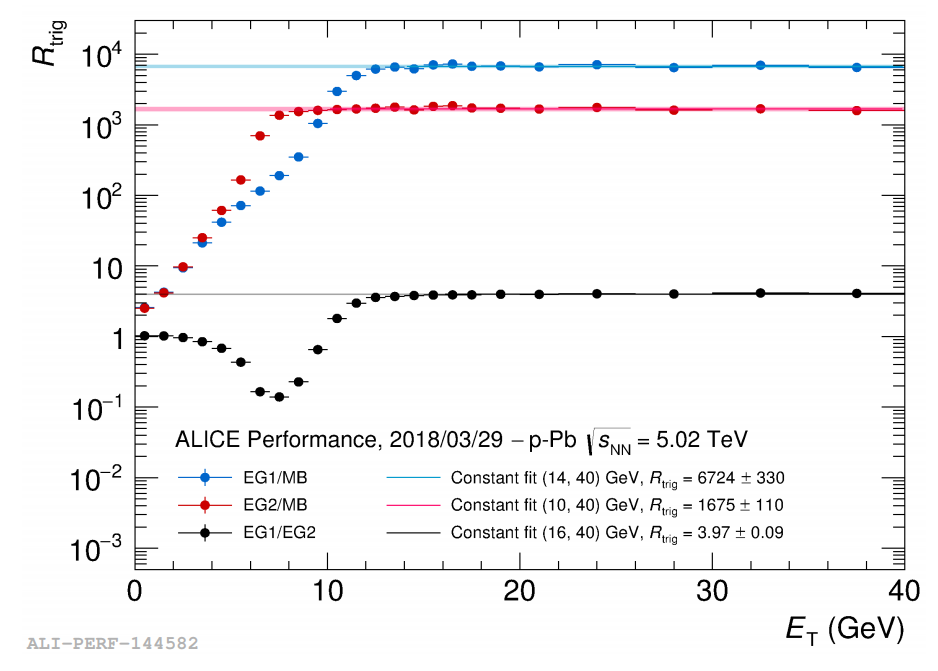
\includegraphics[width=0.6\textwidth]{Datasets/RejectionFactorpPb2013}
%\caption{Rejection factor curves for the 2013 p-Pb period (13def). Source: Ref.~\cite{Erwann}.}
%\label{fig:RejectionFactorpPb}
%\end{figure}


%The total integrated luminosity of the 2013 p-Pb sample is about {4.6 nb$^{-1}$} {($\times$ $A$ = 967 nb$^{-1}$ pp equivalent luminosity)} and about {300 nb$^{-1}$} for the 2017 pp sample. Note that the DCal increases the geometrical acceptance for photons by roughly a factor of 1.3; therefore, comparable statistics of high-$\pt$ photons are expected for pp and p-Pb data.~\footnote{This is the first hard-probes analysis in ALICE that has similar statistics in the reference pp data at the same center-of-mass energy, and thus does not need to rely on extrapolations.}








\section{Monte Carlo simulations}
\label{sec:mcsimulations}
We use Monte Carlo (MC) simulations to obtain the signal shower-shape distributions for the template fits (section~\ref{sec:purity}) and to study tracking performance (section~\ref{sec:tracking}).

The simulations of hard processes are based on the \textsc{Pythia} event generator. In \textsc{Pythia}, the signal events are included via $2\to2$ matrix elements with $gq\to\gamma q$ and $q\bar{q}\to\gamma g$ hard scatterings, defined at the leading order, followed by the leading-logarithm approximation of the partonic shower. The soft underlying events in pp collisions as well as fragmentation are included with the default \textsc{Pythia} models. 

For the simulation of \pPb~events, the pp samples are embedded into \pPb~inelastic events generated with \textsc{DPMJET}. The boost of $\Delta y=+0.465$ in the direction of the proton beam is reproduced. % to reproduce the experimentally measured global \pPb~event properties. 

Table~\ref{tab:MCsamples} shows the MC simulations used in this analysis. Each sample is simulated with the detector configuration appropriate for the runs used in this analysis. 

\begin{table}[h]
   \centering
   \caption{Monte Carlo simulations used in this analysis.}
   \label{tab:MCsamples}
   \begin{tabular*}{1.0\columnwidth}{@{\extracolsep{\fill}}llcc@{}}
    \hline
        Name  & Configuration & JIRA ticket link \\
        \hline        
 17g6a1	 &\pPb, 5 TeV, \textsc{Pythia8} Gamma-Jet +DPMJET anchored to 13d,e,f& \href{https://alice.its.cern.ch/jira/browse/ALIROOT-7271}{ALIROOT-7271}\\
 17g6a3	 &\pPb, 5 TeV, \textsc{Pythia8} Jet-Jet +\textsc{DPMJET} anchored to 13def& \href{https://alice.its.cern.ch/jira/browse/ALIROOT-7271}{ALIROOT-7271}\\
  13b2    &\pPb, 5 TeV, \textsc{Dpmjet} anchored to LHC13b,c & \href{https://alimonitor.cern.ch/productions/3996/tag.html}{39374}\\
 18b10a(b)\_calo	 &pp 5 TeV, \textsc{Pythia8} Gamma-Jet anchored to 17p/q& \href{https://alice.its.cern.ch/jira/browse/ALIROOT-7692}{ALIROOT-7692}\\
 18l2a(b)     &pp 5 TeV, \textsc{Pythia8} Jet-Jet anchored to 17p/q& \href{https://alice.its.cern.ch/jira/browse/ALIROOT-8144}{ALIROOT-8144}\\
   
                 \hline
   \end{tabular*}
\end{table}
\FloatBarrier

\section{Event selection}
\label{sec:eventselection}
We use the following event selection criteria to ensure good event quality and uniform acceptance:
\begin{itemize}
\item Run passes QA for EMCal and ITS (the selected runs are listed in Table~\ref{tab:datasets}).
\item At least one EMCal cluster with $\pt>12$ \GeVc.
\item Selected at least one of the EMCal triggers (logical OR of the trigger strings listed in Table~\ref{tab:triggerstrings}).  %(low and high thresholds).
\item Valid vertex ($|z|\neq0.0$) and $|z|<10$ cm 
%\item Pileup rejection (\textsc{IsPileupFromSPD}(5, 0.8)=False).
\end{itemize}

Where the EMCal is mentioned, we use the same criteria on the DCal (used in the 17q dataset). We use EMCal in text for brevity.
The number of events that pass our selection in each sample is shown in Table~\ref{tab:eventsselected}. We report the events selected for each trigger separately, as well as the logical OR combination. In \pPb~events, the number of events is dominated by the EG1 trigger (11 \GeVc~threshold), and by the EG2 trigger (5 \GeVc) in pp collisions. 

\begin{table}[h]
   \centering
   \caption{Number of events that passed our full event selection for each of data taking period used in this analysis. The numbers are also shown separately for EG1 (DG1) and EG2 (DG2) triggers.}
   \label{tab:eventsselected}
   \begin{tabular*}{1.0\columnwidth}{@{\extracolsep{\fill}}llll@{}}
    \hline
    Dataset &  	N$^{\mathrm{EG1||EG2}}$ &	N$^{\mathrm{EG1}}$ & N$^{\mathrm{EG2}}$\\
    \hline
    13d &	134024 & 133326 & 12528\\
    13e &	198108 & 196745 & 22409\\
    13f &   340607 & 338198 & 38353\\
    13f\_new & 241870 & 240074 & 30310\\
%    Dataset &  	N$^{\mathrm{EG1||EG2||EJ1||EJ2}}$ &	N$^{\mathrm{EG1}}$ & N$^{\mathrm{EG2}}$ &	N$^{\mathrm{EJ1}}$  &	N$^{\mathrm{EJ2}}$ \\
%    \hline
%    13d &	173583 & 133326 & 12528 & 122168 & 20917\\
%    13e &	206833 & 196745 & 22409 & 167651 & 3063\\
%    13f &   365775 & 347684 & 40133 & 296144 & 6501\\
%    13f\_new & 252738 & 240074 & 30310 & 204298 & 5110\\
    \hline
    Dataset &	N$^{\mathrm{EG2 || DG2}}$ &		N$^{\mathrm{EG2}}$ & N$^{\mathrm{DG2}}$\\
    \hline

    17q & 406934 & 301086 & 119498 \\
 
    \hline
   \end{tabular*}
\end{table}

%\begin{table}[h]
%   \centering
%   \caption{Number of events with at least one EMCal or DCal cluster with $\pt > 12 GeV/c$ for the pp period. The columns with the label \textit{filtered} refers to the numbers to events which passed our trigger selection, vertex cut, and pile up cut.}
%   \label{tab:eventsselected_pp}
%   \begin{tabular*}{1.0\columnwidth}{@{\extracolsep{\fill}}lllllll@{}}
%    \hline
%    Dataset & N$^{EG2 or DG2}$ &	N$_{filtered}^{EG2 or DG2}$ &	N$^{EG2}$ & N$^{DG2}$ &	N$^{EG2}_{filtered}$ & N$^{DG2}_{filtered}$\\
%    \hline
%    %17q &	406933 &	304621 &	301086	&	257767	&	119499	&	102242\\
%    17q & 937949 &	727234 & 685402 & 279146  &	536212 &	218255\\
%    \hline
%    \textbf{pp} &	937949 &	727234 & 685402 & 279146  &	536212 &	218255\\
%    \hline
%   \end{tabular*}
%\end{table}
\FloatBarrier
\section{Calorimeter cluster reconstruction}
\label{sec:clusterselection}
\subsection{Definition}
EMCal clusters are formed by a clustering algorithm that combines signals from adjacent towers. We use calorimeter clusters defined with the ``V1'' algorithm. This algorithm starts from a ``seed" cell, found from a local-maximum scan, and adds ``neighbor" cells to the cluster if they are above a given threshold. The cluster definition is exclusive, i.e. once a cell is assigned to a cluster, it is not considered for other clusters. The minimum energy for the seed and neighbor were set to 500 and 100 MeV respectively; these values are several times larger than the standard deviation of the electronic noise\footnote{Some photon analysis use a 50 MeV threshold, but 100 MeV has been found to improve cell time measurements. The 100 MeV threshold has been used for example in Ref~\cite{Acharya:2017tlv}.}.

\subsection{Corrections}
We apply several corrections at the cell level, implemented within the ``EMCal Correction Framework,"\footnote{\url{http://alidoc.cern.ch/AliPhysics/master/_r_e_a_d_m_eemc_corrections.html} } before the clustering algorithm is run over the data and simulations. The following corrections are applied: 
\begin{itemize}
\item ``\textsc{CellEnergy}"\\
This performs an energy calibration of cells, with coefficients obtained with $\pi^{0}\to\gamma\gamma$ mass measurements.
\item ``\textsc{CellBadChannel}''\\
This removes cells that declared hot or dead for a given run period. 
\item ``\textsc{CellTimeCalib}"\\
This correction applies constant offsets, which are arbitrary, to the cell time measurements to minimize the spread among cells. 
\item ``\textsc{CellEmulateCrosstalk}''. \\
This correction, described in detail in Ref~\cite{CrossTalk}, modifies the simulated cell energies to emulate the cell cross-talk that has been observed in data. This is applied to all the simulations described in Table~\ref{tab:MCsamples}. 
\end{itemize}

\subsection{Selection}
The following selection is applied on the resulting clusters\footnote{This event selection also closely follows previous and concurrent isolated-photon spectra analyses in pp and \pPb~ data.}:

\begin{itemize}
\item Cluster $\pt$ cut:  $12< \pt < 40$ \GeVc.
\item Cluster pseudorapidity: $|\eta| <0.67$\\
The cluster pseudorapidity is corrected for the position of the primary interaction vertex. 
\item Number of cells cut: $N_{\mathrm{cell}}\geq2$\\
This requirement removes clusters that are likely dominated by noise. 
\item Exoticity cut: $E_{\mathrm{cross}}/E_{\mathrm{cluster}}$ $> 5\%$\\
We remove ``exotic'' or ``spiky'' clusters likely coming from slow neutrons or highly-ionizing particles hitting the avalanche photo-diode of a cell by a requirement on the ratio of the summed energy around the leading cell to the total cluster energy.
\item Cluster time cut:  $|t|<20$ [ns]\\
We require a cluster time measurement of $|t|<$ 20 ns to remove out-of-bunch pileup. 
\item Number of local maxima cut: $N_{LM}<$ 3\\
This cuts suppresses background and improves the MC simulation description of the background~\cite{Acharya:2019jkx}.  
\item Distance seed-cell to bad-channel$\geq 1$ cells.
\end{itemize}

Figures~\ref{ClusterCutFlow_pPb} and~\ref{ClusterCutFlow_pp} show the distribution of the variables used in the cluster selection and the effect of sequential selection (``cut flow") for the \pPb~and pp data respectively. Table~\ref{tab:photonCutFlow} shows a summary of the effect of sequential selection on the number of selected clusters in both pp and \pPb~data. 

\begin{figure}[h]
\center
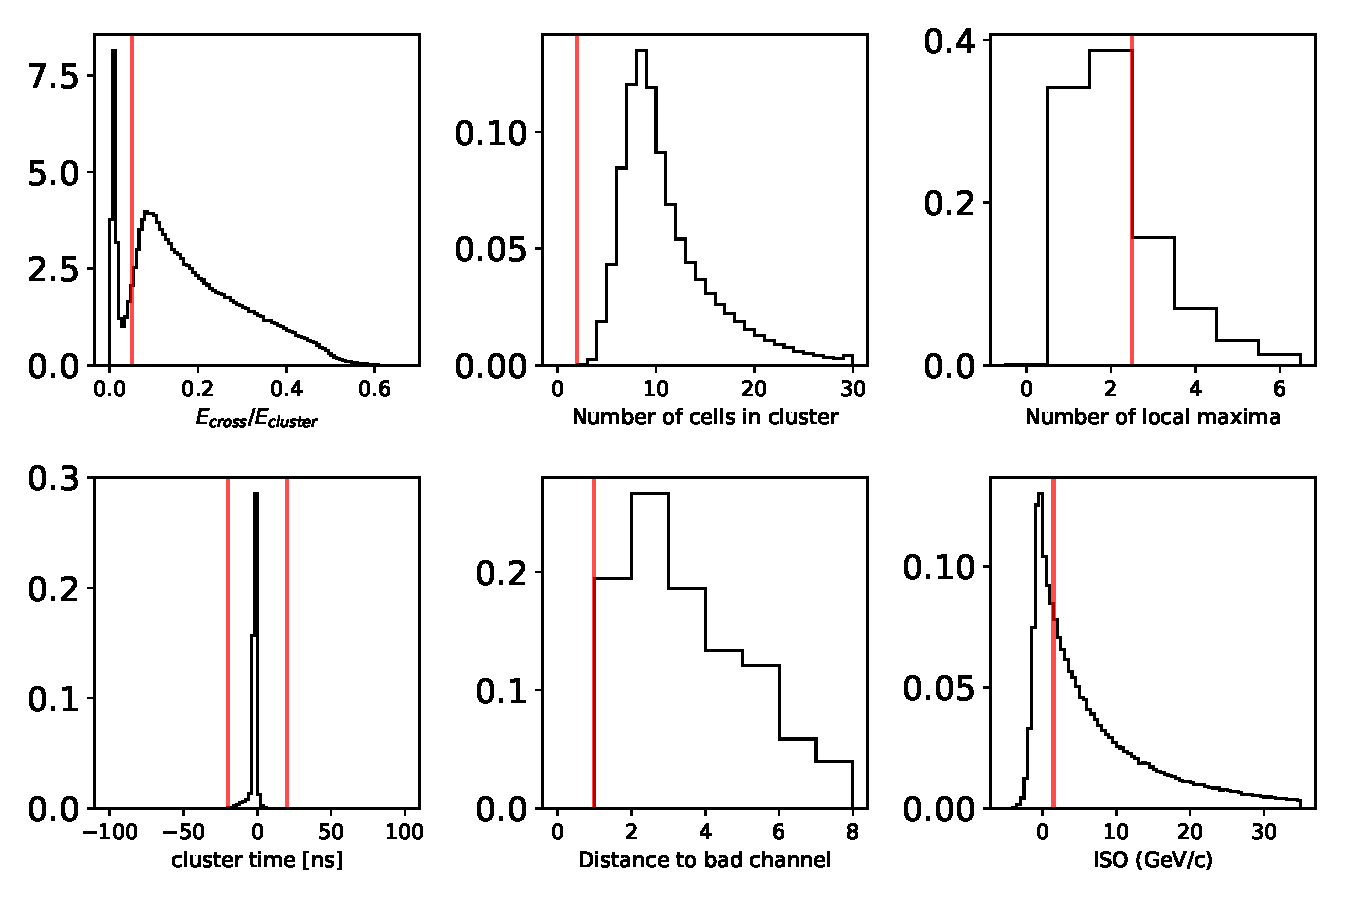
\includegraphics[width=0.95\textwidth]{EventAndClusterSelection/ClusterCutFlow_dataset_Skimmed_13def}
\caption{Distribution of variables used in the cluster selection of \pPb~data. The red vertical lines represent the cuts used. The cluster cuts get applied sequentially, i.e. the clusters cut with a given variable do not appear in the next.}
\label{ClusterCutFlow_pPb}
\end{figure}


\begin{figure}[h]
\center
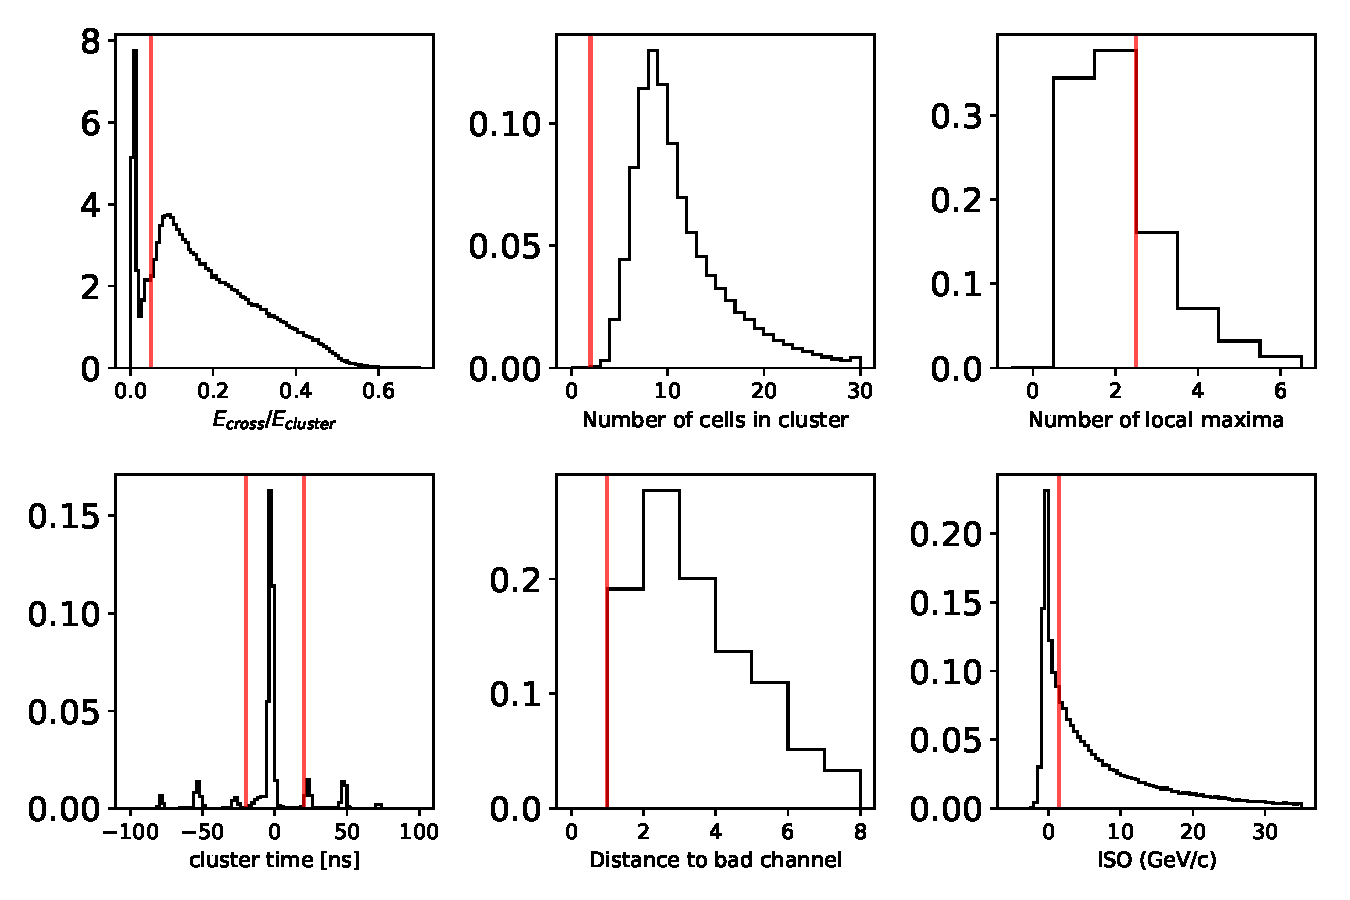
\includegraphics[width=.95\textwidth]{EventAndClusterSelection/ClusterCutFlow_dataset_Skimmed_17q}
\caption{Distribution of variables used in the cluster selection in pp data. The red vertical lines represent the cuts used. The cluster cuts get applied sequentially, i.e. the clusters cut with a given variable do not appear in the next.}
\label{ClusterCutFlow_pp}
\end{figure}


\begin{table}[h]
   \centering
   \caption{Number of clusters, with  $12<\pt<40$ \GeVc, that pass our selection in 2013 \pPb~and 2017 pp data.}
   \label{tab:photonCutFlow}
   \begin{tabular*}{1.0\columnwidth}{@{\extracolsep{\fill}}lcc@{}}
    \hline
       Selection  &  \pPb~ data & pp data  \\
       \hline
       $|\eta| < 0.67$& 714834 & 385220  \\
      $E_{\mathrm{cross}}/E_{\mathrm{cluster}}$ $> 5\%$ & 613560 & 323750   \\
       $N_{\mathrm{cell}}$ $\geq 2$   &613560& 323750       \\
              $N_{LM}<$ 3 & 443102&231490 \\
       $|t|<20$ [ns] &441639 & 171470  \\ 
       Distance-to-bad channel $\geq 1$ &441639  &171470  \\ 
       $\iso<$  1.5~\GeVc & 137895  & 58638 \\ 
       0.1 $< \sigma^2_{\textrm{long}}<$  0.3  & 40027 & 16628  \\ 
       \hline
	   %Total clusters passing $\gammaiso$ selection & 38415  & 16,586 %\\ 
       %\hline
   \end{tabular*}
\end{table}

%Table~\ref{tab:mcCutFlow} shows a summary of the effect of sequential selection on the number of selected clusters in various simulated samples. This shows that in simulation, a much larger fraction of the total number of clusters passes the exoticity cut than in data. This is attributed to the fact that the simulation does not describe the albedo neutrons or energetic particles hitting the APD of the cell readout. The dijet simulation describes the cut flow relatively well, including the number of local maxima and the isolation criteria that is described in detail in Section~\ref{sec:isolation}.

%\begin{table}[h]
%\vspace*{0cm}
%   \centering
%   \caption{Fraction of clusters, with  $12~\GeVc < \pt < 30$ \GeVc, that pass our selection in simulated data. The percentage refer to the sequential application of each cut.}
%   \label{tab:mcCutFlow}
%   \hspace*
%   {-2.8cm}\begin{tabular}{@{\extracolsep{\fill}}lcccc@{}}
%    \hline
%    &  Pythia $\gamma$-jet + UE & Pythia dijet-jet + UE &  Pythia $\gamma$-jet & Pythia dijet-jet\\
%    &   17g6a1 & 17g6a3 & 18b10a(b)\_calo & 18g7a(b)\_calo\\ \hline
%    $|\eta| < 0.67$&  100$\%$ & 100$\%$ & 100$\%$ & 100$\%$\\
%    $E_{\mathrm{cross}}/E_{\mathrm{cluster}}$ $> 5\%$ & 97$\%$ & 97.8$\%$ & 97.5$\%$ & 96.3$\%$\\
%    $N_{\mathrm{cell}}$ $> 2$    &  99.9$\%$ & 100$\%$ & 100$\%$    & 100$\%$ \\
%
%	$|t|<20$ [ns] & 100$\%$ & 100$\%$ & -$\%$ & -$\%$ \\ 
%	Number of local maxima $< 3$ & 98.4$\%$ & 88.9$\%$ & 87.8$\%$ & 64.2$\%$\\ \hline
%    Fraction that pass all cuts above& 95.4$\%$ & 86.9$\%$ & 85.6$\%$ & 61.8$\%$ \\ \hline 
%	Fraction that pass all cuts above that also pass ISO cut& 91.1$\%$ & 40.3$\%$ & 86.8$\%$ & 14.6$\%$ \\ 		\hline
%    Fraction that pass all cuts & 86.9$\%$ & 35.0$\%$ & 74.3$\%$ & 9.0$\%$ \\ \hline 
%   \end{tabular}
%\end{table}
%Tables fractions need to be remade with latest MC samples. 


%\subsection{Selection Efficiency}
%The efficiency for the combined effect of all the selection cuts we used, with the exception of the isolation selection that is discussed in more detail in Section~\ref{sec:isolation}, is shown in Figure~\ref{fig:ClusterSelectionEfficiency}. The various efficiencies for the different cases are as follow: \pPb~: 0.91, pp-EMCal+DCal: 0.90, pp-EMCal: 0.91, pp-DCal: 0.79. These efficiencies were obtained by applying a constant fit to each case. 
%\begin{figure}[h]
%\center
%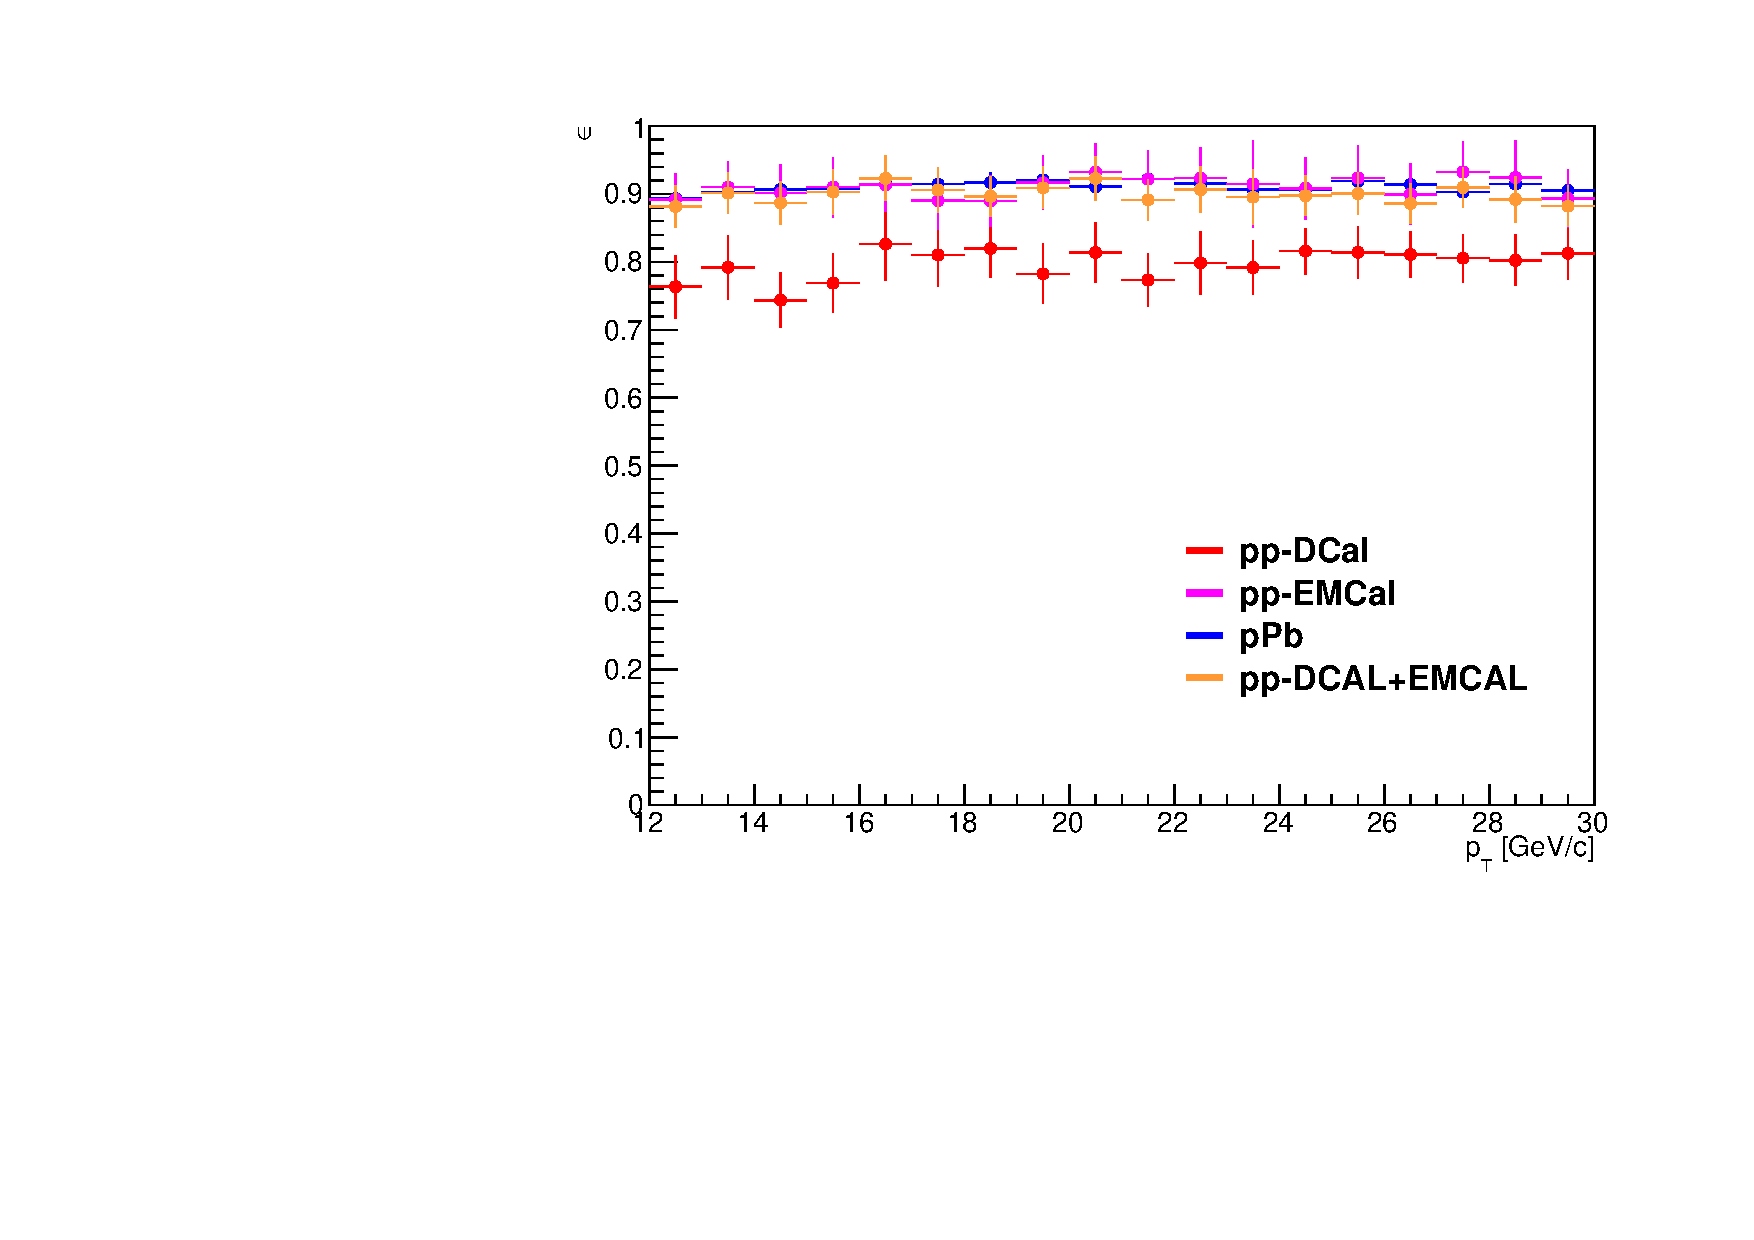
\includegraphics[width=0.5\textwidth]{EfficiencyAppendix/EfficiencyComparison_photons.pdf}
%\caption{Cluster selection efficiency for pp and \pPb~ data taking periods. The error bar represents statistical uncertainty only.}
%\label{fig:ClusterSelectionEfficiency}
%\end{figure}

%We do not use this efficiency in our analyzes because we report quantities normalized to the number of photons. However, in principle the efficiency could enter as a second-order bias if it varied rapidly with $\pt$~and we reported measurements in wide $\pt$~intervals. We note from Figure~\ref{fig:ClusterSelectionEfficiency} that this is not the case, i.e. the efficiency is almost constant for the $\pt$~range analyzed here.

%The number of cells in the cluster peaks at around 8 and has a tail to larger values, but a spike at low values; the requirement of $N_{\mathrm{cell}}>2$ removes about 10$\%$ of the clusters. The $E_{\mathrm{cross}}/E_{\mathrm{cluster}}$ variable peaks at around 0.1 and has a smooth tail to larger values that reach up to around 0.6. A peak at small values is attributed to ``exotic'' clusters that are the product of albedo neutrons or minimum-ionizing particles hitting the APD of the cell, which producing large signal in a single cell but not in their neighbors~\cite{ExoticClusters}. The exoticity cut, $E_{\mathrm{cross}}/E_{\mathrm{cluster}} >$ 0.03 rejects about 6\% of all clusters. The time cut rejects less than 1$\%$ of the clusters in \pPb~, but about a quarter in the pp dataset. Then, we reject events with more than 2 local minimum to reduce background from meson decays and hadrons, rejecting about 20\% of the remaining clusters. 
%Finally, we apply an isolation cut (described in Section~\ref{sec:isolation}) to reduce background from multi-jet events; this keeps about a third of all the clusters. 


\FloatBarrier

\section{Photon Identification}
\label{sec:photonID}
Photons from $\pi^0$ decays begin to merge into a single cluster in the EMCal above approximately  6~\GeVc. To identify clusters produced by single photons and reject clusters produced by two photons from a meson decay, we use variables that encode the shape of the calorimeter shower. %measured in the EMCal and DCal. We use the $\lambdasquare$ variable and a novel neural network variable; these are described in the next sections.

\subsection{Shower-shape variable}
The $\lambdasquare$ variable is the weighted root-mean-square of the shower energy along the major ellipse axis, defined according to~Ref.~\cite{Abelev:2014ffa} as:
\begin{equation}
\lambdasquare = \frac{s_{\eta\eta}+ s_{\phi\varphi}}{2} + \sqrt{   \frac{(s_{\eta\eta} - s_{\phi\varphi})^{2}}{4} + s^{2}_{\eta\varphi}         },
\end{equation}
where $s_{ij} = \langle ij \rangle - \langle i \rangle\langle j \rangle$ are the covariance matrix elements; the $i,j$ are cell indices in $\eta$ and  $\varphi$ axes; $\langle ij \rangle$ and $\langle i\rangle$, $\langle j\rangle$ are the second and the first moments of the cluster position cell weighted as follows:
\begin{equation}
\mathrm{weight} = \mathrm{max}\left(\log(E_{\mathrm{cell}}/E_{\mathrm{cluster}}), w_{0}\right). 
\end{equation}

Following previous work~\cite{Acharya:2018dqe}, we chose the cutoff in the log-weighting as $w_{0}=-4.5$, which means that cells that contain less than {$e^{-4.5} =$ 1.1$\%$} of the total cluster energy are not considered in the $\lambdasquare$ calculation.

Since $\lambdasquare$ represents the extent of the cluster, it discriminates between clusters belonging to single photons, for which the $\lambdasquare$ distribution is narrow and symmetric, and merged photons from neutral-meson decays, for which the distribution is dominated by a long tail towards higher values. 

%\subsection{Comparison of cluster distributions in pp and p-Pb data}
%Figure~\ref{fig:ppandpPbcomparison} shows a comparison between the transverse momentum and shower-shape distributions ($\lambdasquare$, DNN and $E_{\mathrm{max}}/E_{\mathrm{cluster}}$) in pp and p-Pb data for clusters that pass our selection. The distributions overlap to a large degree (at approximately the percent level), suggesting that the photon identification performance in both data taking periods is fairly similar even though they are separated by more than 4 years and the detector configurations are different (the DCal was installed in Run-2). This also severely constrains the degree of performance degradation due to higher underlying event density in p-Pb collisions. 

%\begin{figure}[h]
%\center
%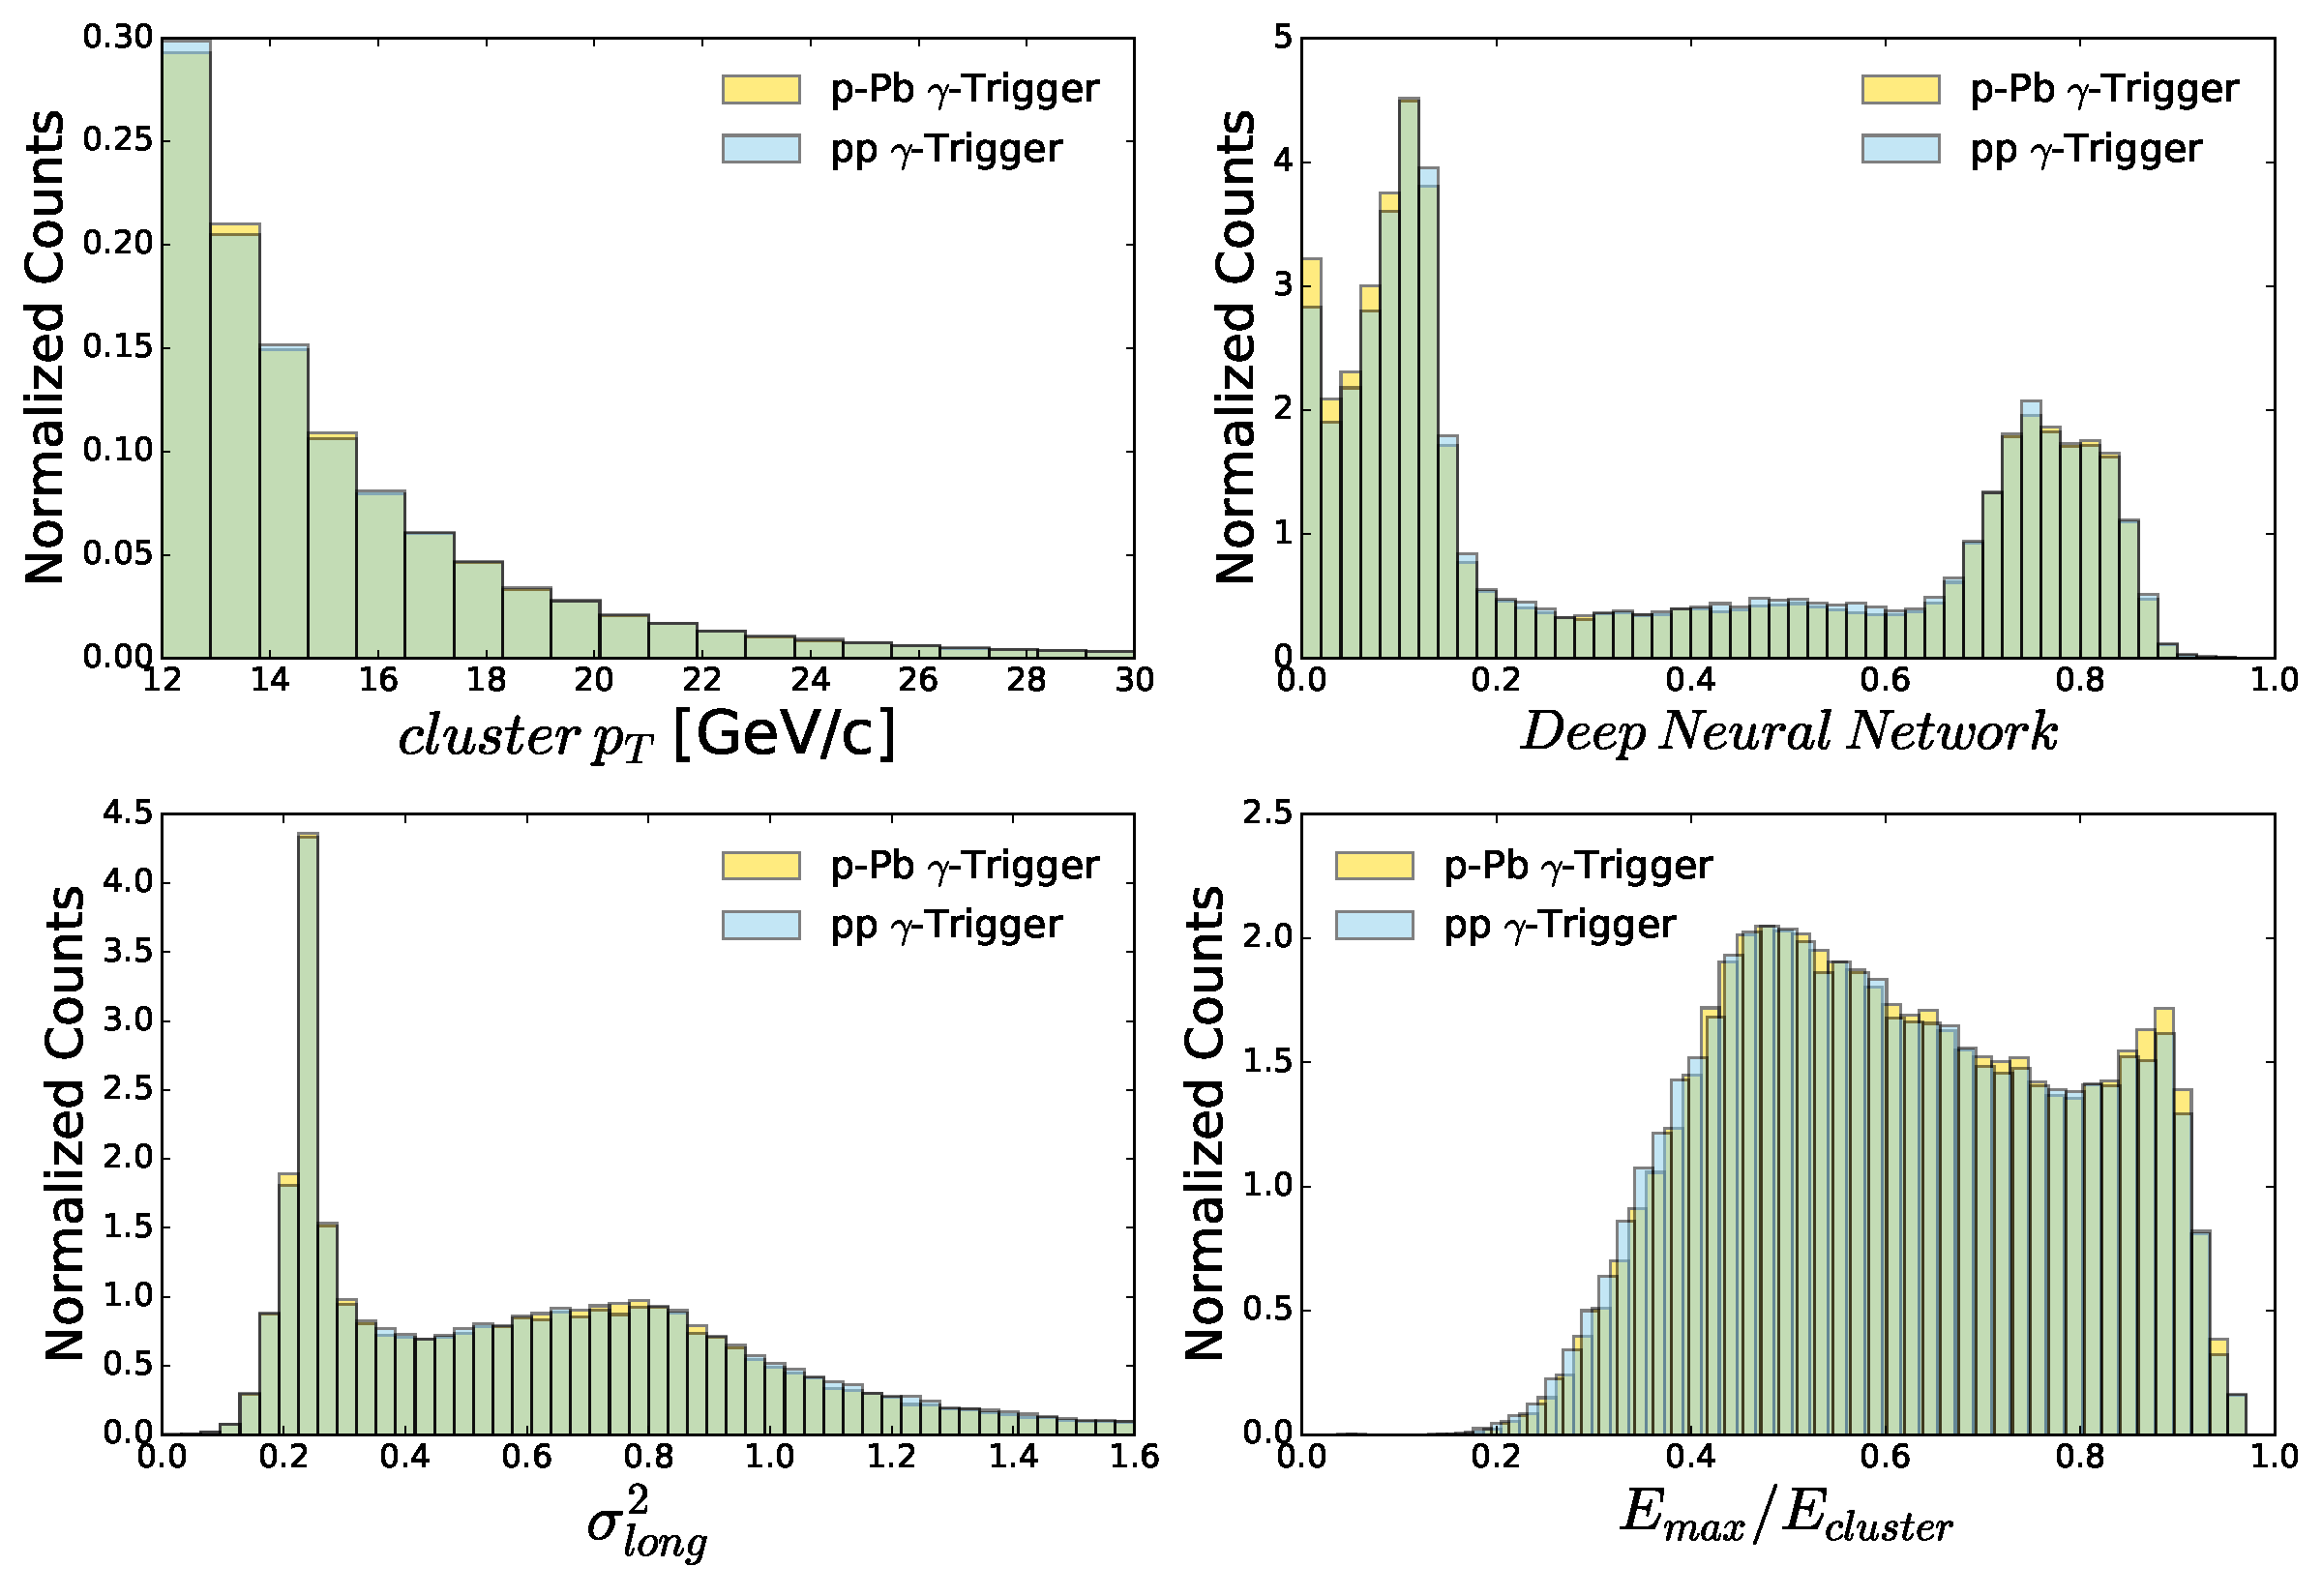
\includegraphics[width=0.9\textwidth]{EventAndClusterSelection/ppandpPbvariables.pdf}
%\caption{Transverse momentum and shower shape distributions for clusters that pass our selection in pp and p-Pb photon-triggered data. The overlap of the histograms is shown in green.}
%\label{fig:ppandpPbcomparison}
%\end{figure}

%\subsection{Comparison of cluster distributions in EMCal and DCal}
%Figure~\ref{fig:EMCALandDCALcomparison} shows a comparison between the transverse momentum and shower-shape distributions for clusters measured in EMCal and DCal in pp data. 
%\begin{figure}[h]
%\center
%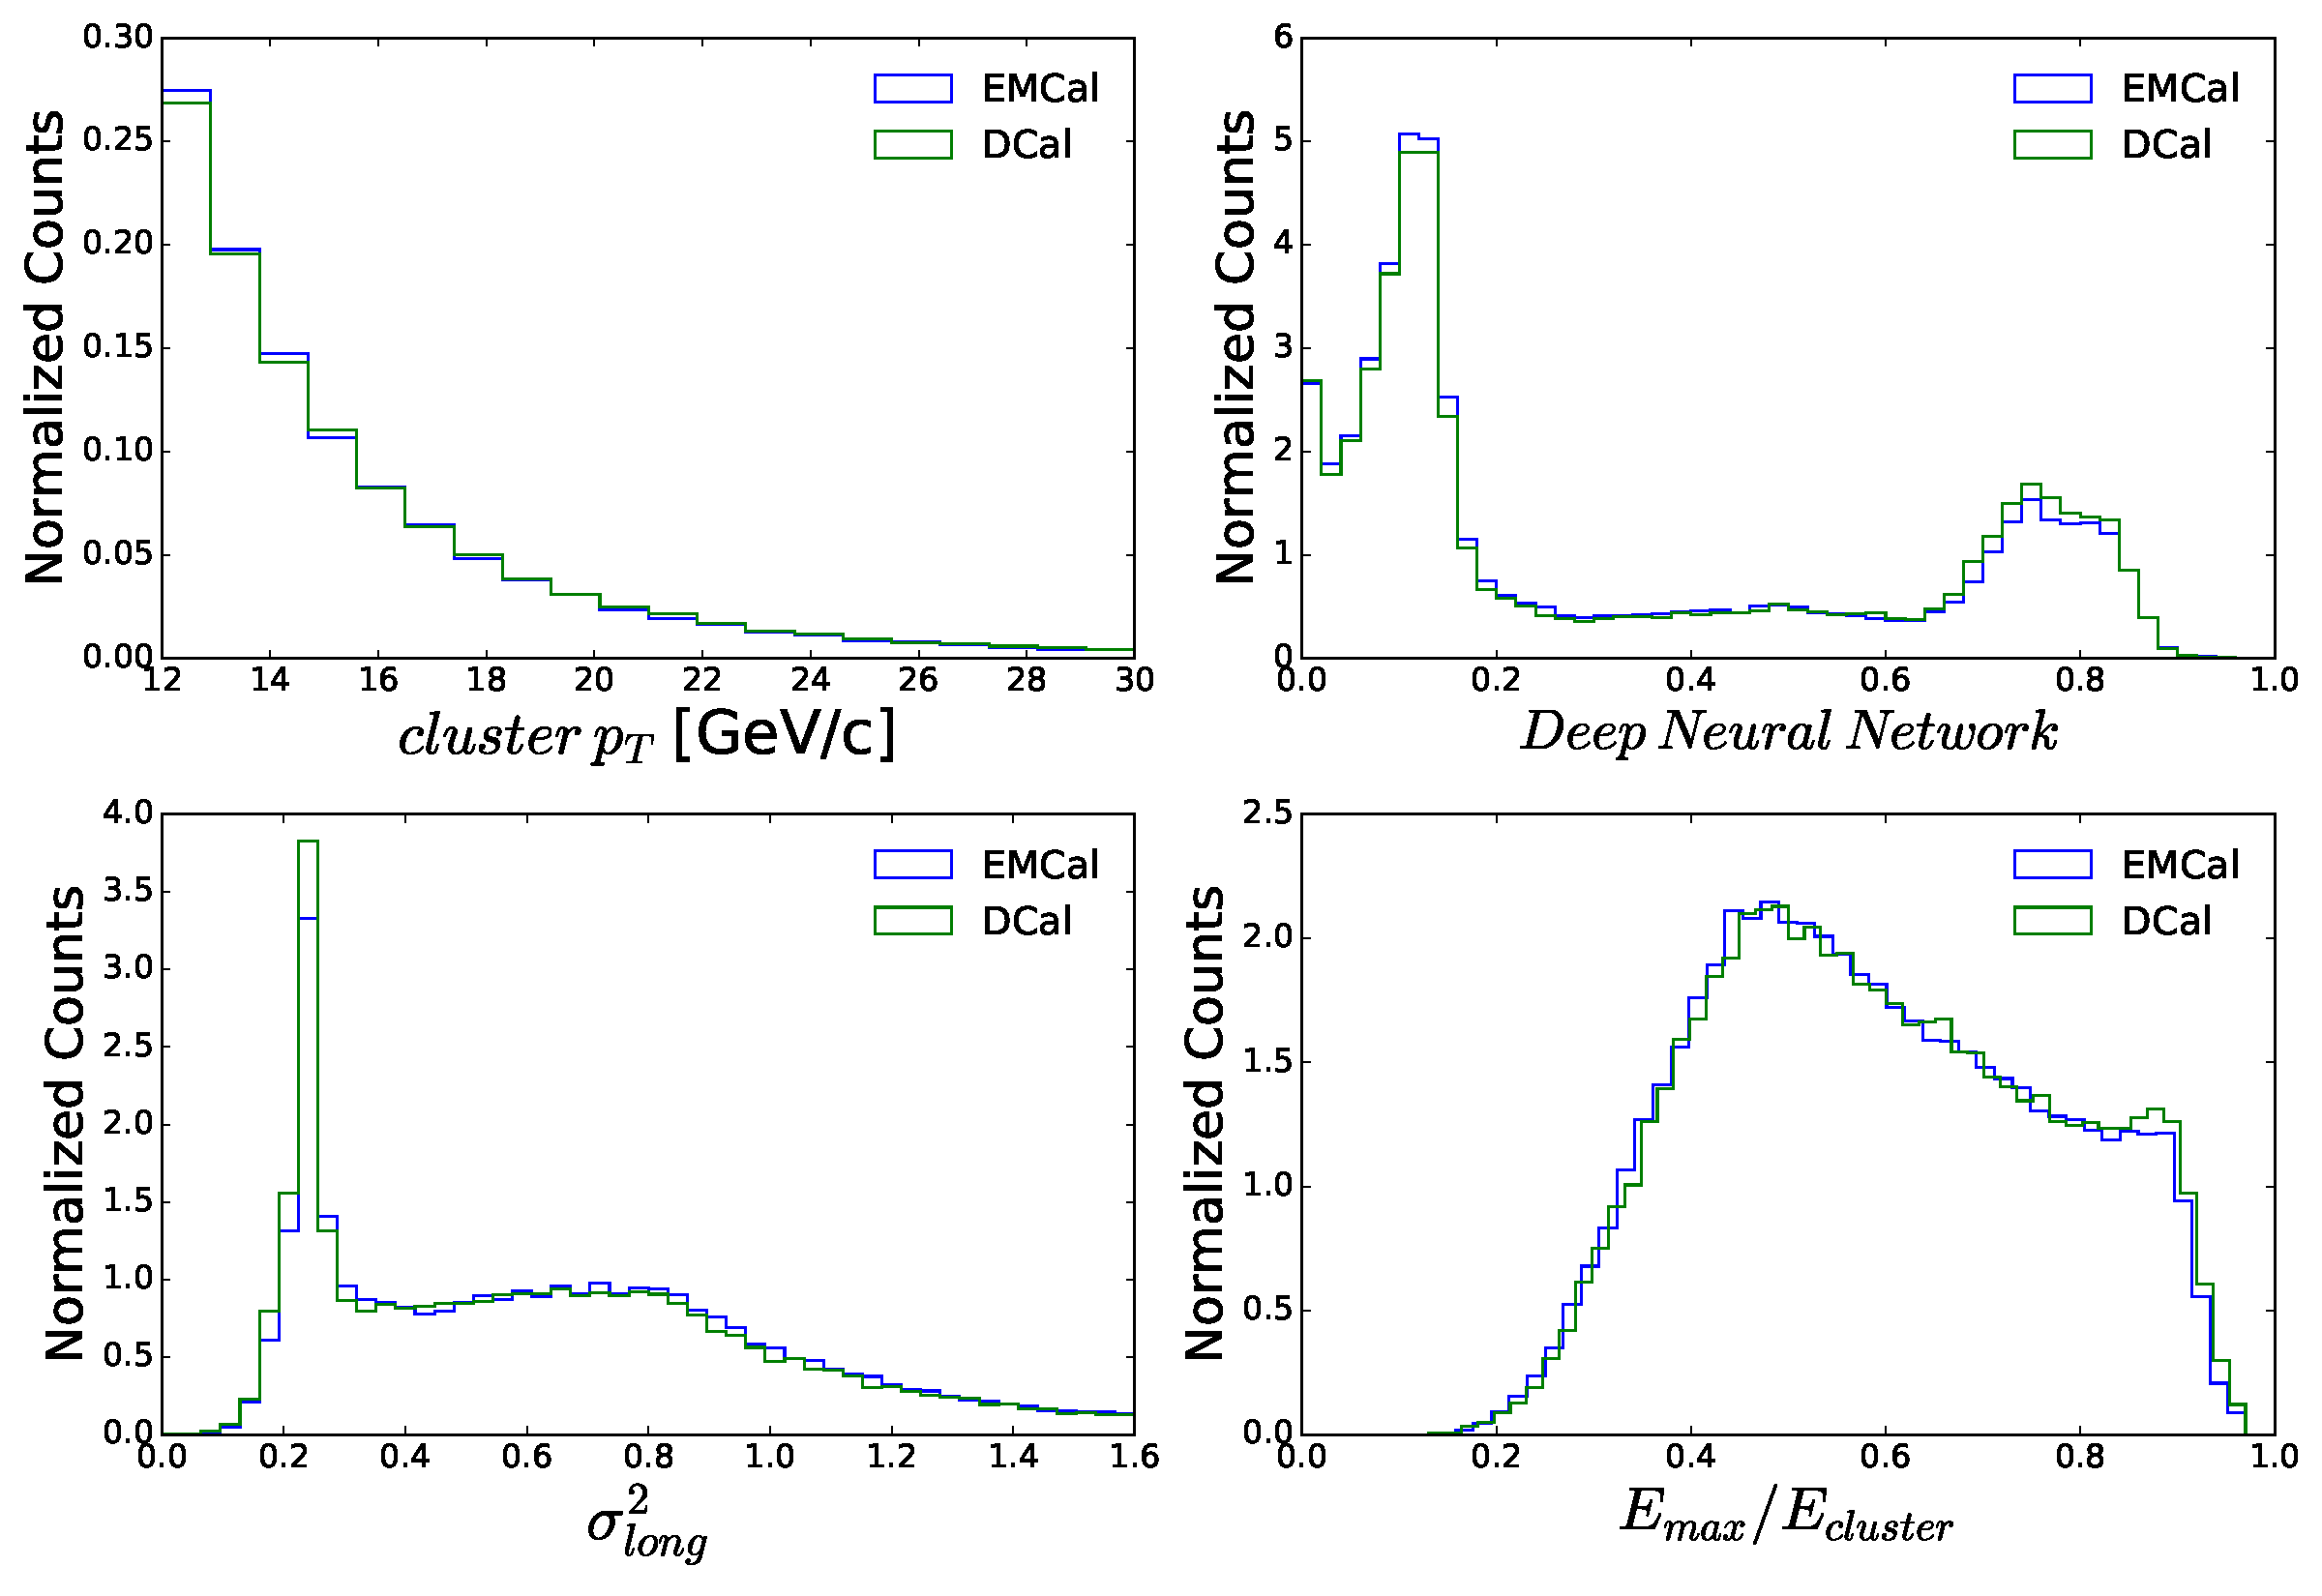
\includegraphics[width=0.9\textwidth]{EventAndClusterSelection/EMCAL_DCAL_variables.pdf}
%\caption{Transverse momentum and shower shape distributions for EMCal and DCal measured %clusters in pp photon-triggered data.}
%\label{fig:EMCALandDCALcomparison}
%\end{figure}

%The transverse momentum distributions are practically the same, which indicates that the EMCal and DCal absolute energy scales are very similar (otherwise a slope change would be expected). However, small but statistically significant differences in the shower-shape variables are observed. This is not surprising, given that is known that previous analyses have reported differences in the shower-shape measured for different super-modules. This is an effect that is attributed to cross-talk among the calorimeter cells, and is taken into account in the simulation, as shown in Section~\ref{sec:clusterselection}. 



%%%%%\subsection{Deep Neural Network}
%\label{sec:deepneuralnetwork}
%We have utilized a novel machine learning technique to improve the efficiency and purity of separating single and double photon clusters in the EMCal and DCal. Inspired by the similarities between pattern recognition in electromagnetic calorimeters and well-known image recognition problems, we utilize a deep neural network. The open-source neural network software package \textsc{TensorFlow} 1.7.0 was used~\cite{tensorflow2015-whitepaper}, first on a laptop, and then on the Cori supercomputer at NERSC~\cite{doi:10.1002/cpe.4291}.

%The neural network takes as input a $5\times 5$ array of the cells around each cluster's maximum cell. These 25 pieces of information, plus the cluster $\eta$, 1/$\sqrt{E_{\mathrm{cluster}}}$, the signed $\Delta\phi$ distance of the cluster to the closest supermodule center, and the V0M multiplicity, yield 29 parameters per cluster. We checked whether the neural network discrimination improves upon using a larger cell array, but found that 5x5 is sufficient. The $\eta$ and $\Delta\phi$ distance to the closest supermodule center are included to parametrize the residual nonprojectiveness, and possible alignment issues, while the V0M multiplicity enables the neural network weights to be applied across pp and p-Pb datasets (with possible extension to PbPb data).

%We utilized a neural network with 4 fully connected layers with 50 neurons each. After the 4th layer, 2 probabilistically motivated output neurons are formed from the output activations of the 4th layer, via the softmax function. One of these two neurons is tapped as the single photon discriminant.

%The neuron consists of the weight (a matrix multiplied with the input vector), a bias (the vector added after the matrix multiplication) and a suitable activation function. During the course of training, the each neuron learns an "activation", which is a real number usually close to $\pm 1$. Hence, a single neuron without the activation function is a linear classifier. The activation function -- termed analogously to the function of the firing rate in a biological neuron -- is needed to produce nonlinear classification.

%For this analysis, a Rectified Linear Unit (ReLU) activation function was used. It computes the function $f(x) = max(0,x)$, in effect setting a threshold for the activation at zero. Using a ReLU activation function greatly accelerates the convergence of stochastic gradient descent compared to the sigmoid or tanh functions. It has been argued that this is due to its linear, non-saturating form. However, a large gradient flowing through a ReLU neuron could cause the weights to update in such a way that the neuron will never activate on any datapoint again. If this happens, then the gradient flowing through the unit will forever be zero from that point on. That is, the ReLU units can irreversibly die during training. For example, as much as 40\% of a network can be ``dead'' (i.e. neurons that never activate across the entire training dataset) if the learning rate is set too high. This can be alleviated by making the network sufficiently large to allow for redundancy.

%After four layers, our neural network uses a binary softmax function to create a two-neuron output.  For example, one can interpret $\sigma(\sum_i w_ix_i+b)$
%to be the probability, P, of one of the final two neurons. The probability of the other final neuron would be 1 - P, since they must sum to one.

%The neural network was trained on photons from 8--30 GeV in simulated events, using an EM-enriched pPb Monte Carlo (ALICE LHC17g6a1, $\hat{p}_T$ bin 1--2, and LHC17g6a3, $\hat{p}_T$ bin 1--4, data sets), and 130K clusters each for training and test samples. Training was done using 128 batches and 12 epochs. The training time for each training sample was about 5 minutes on either a GPU or a Intel Knights Landing Xeon Phi.

%\subsection{Verification of DNN in LHC16k (13 TeV pp)}

%In order to confirm that the DNN is truly selecting on single photons, the $\eta \rightarrow \gamma\gamma$ channel in the intermediate ($\approx 10\:\mathrm{GeV}$) can be used to identify prompt single photons. The $\eta$ is optimum for this due to the larger opening angles, so the two decay photons are not merged until higher $p_T$. However, due to the statistics limitation in lower $\sqrt{s}$ (collision systems taken with LHC HI budget), the 13 TeV pp is preferable. We utilize data from LHC16k, which is the largest, triggered run period in 2016.

%For the LHC16k study, the following DPG runs with good TPC and EMCAL performance are selected:
%\begin{quote}
%258537, 258499, 258477, 258456, 258454, 258426, 258393, 258387, 258359, 258336, 258299, 258278, 258274, 258273, 258271, 258270, 258258, 258257, 258256, 258204, 258203, 258202, 258198, 258197, 258178, 258117, 258114, 258113, 258109, 258108, 258107, 258063, 258062, 258059, 258049, 258048, 258045, 258042, 258019, 258017, 258014, 258012, 257963, 257960, 257958, 257957, 257939, 257937, 257936, 257893, 257892, 257855, 257850, 257803, 257800, 257799, 257798, 257797, 257773, 257765, 257754, 257737, 257735, 257734, 257733, 257724, 257697, 257694, 257692, 257691, 257689, 257687, 257682, 257642, 257606, 257605, 257594, 257590, 257587, 257566, 257562, 257561, 257560, 257541, 257540, 257539, 257537, 257531, 257530, 257492, 257491, 257490, 257487, 257474, 257457, 257320, 257260, 257224, 257209, 257206, 257204, 257145, 257144, 257142, 257141, 257140, 257139, 257138, 257137, 257136, 257100, 257092, 257084, 257083, 257082, 257080, 257077, 257026, 257021, 257012, 257011, 256944, 256942, 256941, 256697, 256695, 256694, 256692, 256691, 256684, 256681, 256677, 256676, 256658, 256620, 256619, 256592, 256591, 256589, 256567, 256565, 256564, 256562, 256561, 256560, 256556, 256554, 256552, 256514, 256512, 256510, 256506, 256504
%\end{quote}
%The reconstruction used is pass1.

%For the MC comparison, the LO $\gamma$-jet (since this is where the signal template originates) LHC17i3a1 sample is used, where the first 4 $\hat{p}_T$ are used, and cross section/``ntrials'' merged. The run list consists of the intersection of LHC17i3a1 with the DPG validated LHC16k runs, namely:
%\begin{quote}
%256504, 256506, 256510, 256512, 256554, 256556, 256560, 256561, 256562, 256564, 256565, 256567, 256589, 256591, 256592, 256619, 256620, 256658, 256676, 256677, 256681, 256684, 256691, 256692, 256694, 256695, 256697, 256942, 256944, 257011, 257021, 257077, 257080, 257082, 257084, 257092, 257100, 257136, 257138, 257139, 257140, 257141, 257142, 257144, 257145, 257204, 257206, 257209, 257260, 257474, 257487, 257490, 257491, 257492, 257530, 257531, 257540, 257541, 257560, 257561, 257562, 257566, 257587, 257590, 257605, 257606, 257642, 257682, 257687, 257689, 257697, 257724, 257733, 257735, 257737, 257754, 257765, 257773, 257797, 257798, 257799, 257800, 257803, 257850, 257892, 257893, 257936, 257937, 257939, 257957, 257958, 257960, 258012
%\end{quote}

%Even though it is possible to perform a comparison with the LO photon in the $\gamma$-jet sample, the only origin for track MIP contamination on the LO photon side is initial and final state radiation; thus the contamination will be unrealistically low. For this reason, the same selection to reconstruct $\eta$ is applied also to MC, with the downside that the statistics will be limited.

%Because LHC16k contains pile-up events, for event selection in the data, any event containing a 2nd SPD vertex is vetoed.

%The following standard cluster selection are applied to both data and MC:
%\begin{equation}
%\begin{split}
%N_\mathrm{cell} &\ge 2\\
%0.1 &< \lambdasquare < 0.7\\
%E_\mathrm{cross} &< 0.05 E_\mathrm{max}\\
%\end{split}
%\end{equation}
%To maximally remove MIP contamination, clusters with any tracks within 3 cell distance on the surface of the EMCAL is vetoed. Finally, in order to enhance the diphoton signal, the asymmetry cut
%\begin{equation}
%\left\lvert\frac{E_1 - E_2}{E_1 + E_2}\right\rvert < 0.5
%\end{equation}
%is applied.

%The diphoton mass is split into a signal region with $0.5 < m_{\gamma\gamma} < 0.6\:\mathrm{GeV}/c^2$, and two background regions with $0.325 < m_{\gamma\gamma} < 0.475\:\mathrm{GeV}/c^2$ and $0.625 < m_{\gamma\gamma} < 0.775\:\mathrm{GeV}/c^2$. Because the background appears approximately linear, the signal and background are simply integrated (with the symmetric choice as stated), then normalized by unit $m_{\gamma\gamma}$, and the background distribution subtracted from the signal distribution.

%\begin{figure}[th]
%\centerline{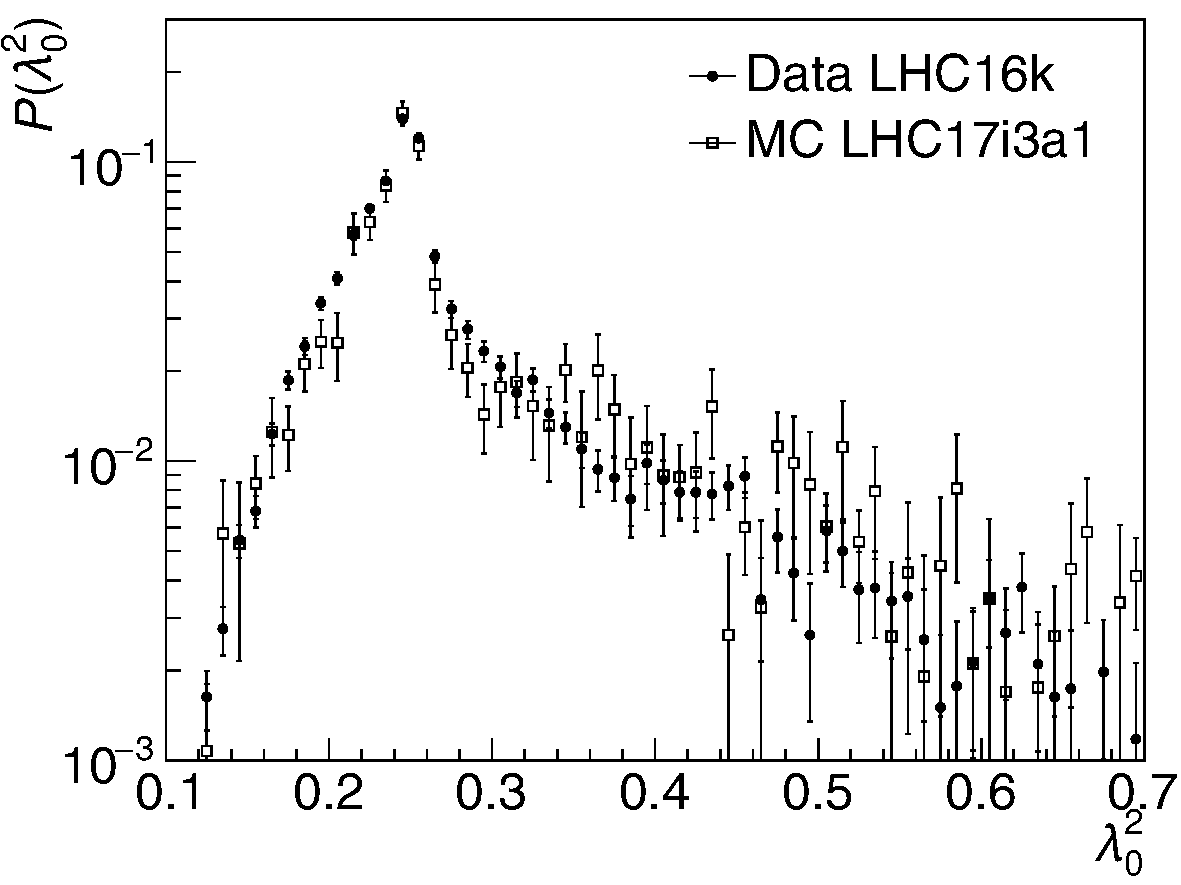
\includegraphics[width=0.3333\textwidth]{eta_lambda02_08_12}%
%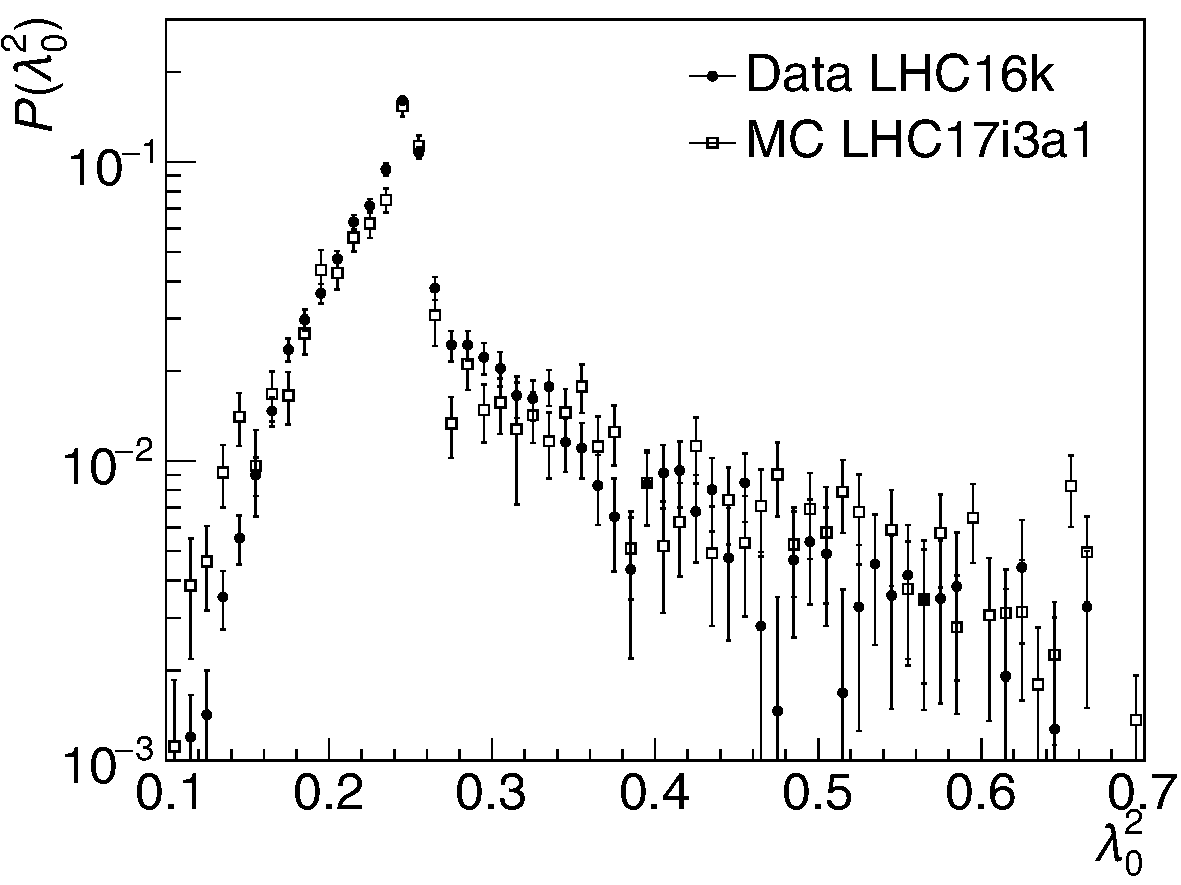
\includegraphics[width=0.3333\textwidth]{eta_lambda02_12_20}%
%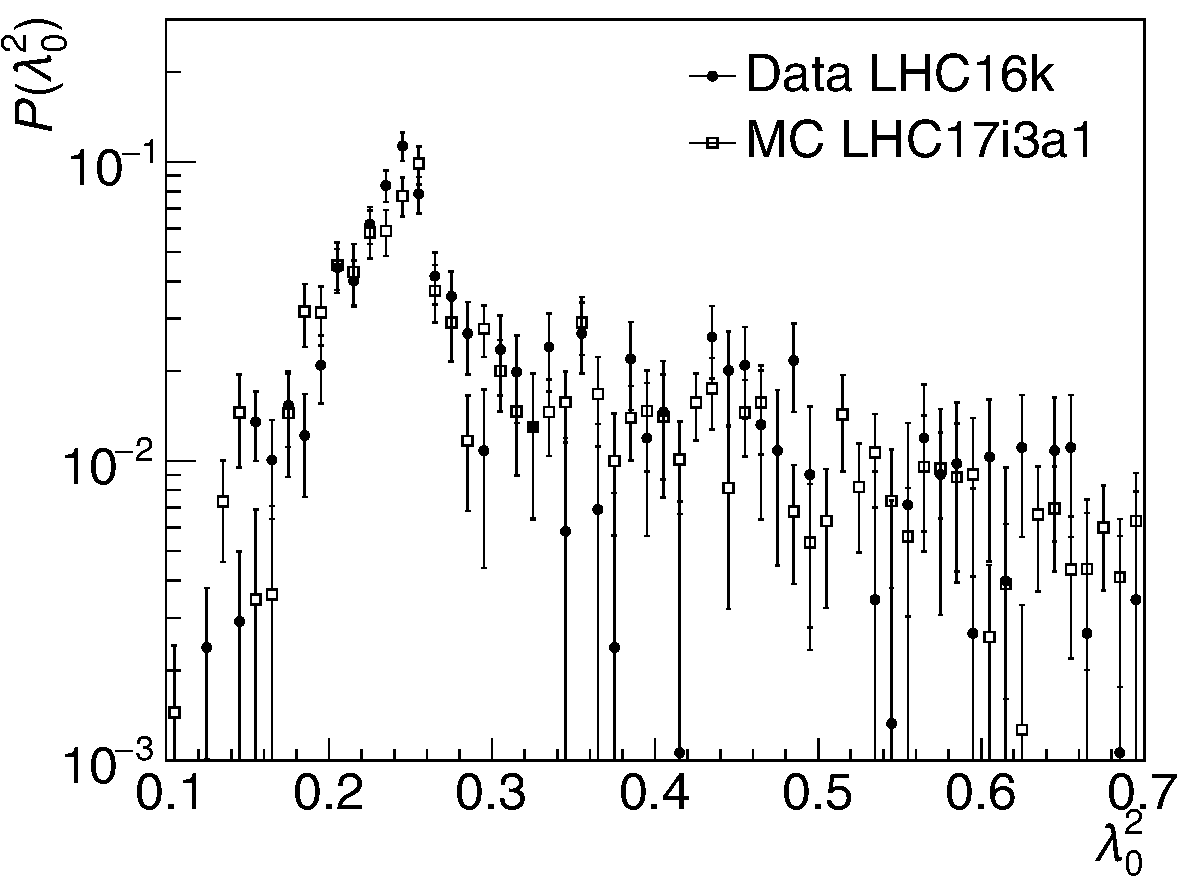
\includegraphics[width=0.3333\textwidth]{eta_lambda02_20_30}}
%\centerline{\hfill$8 \le E_\gamma < 12\:\mathrm{GeV}$\hfill\hfill$12 \le E_\gamma < 20\:\mathrm{GeV}$\hfill\hfill$20 \le E_\gamma < 30\:\mathrm{GeV}$\hfill}
%\centerline{\hfill$\chi^2/\text{DOF} = 1.21$\hfill\hfill$\chi^2/\text{DOF} = 1.82$\hfill\hfill$\chi^2/\text{DOF} = 1.48$\hfill}
%\caption{The distribution of $\lambdasquare$ for single photons, using $\eta \rightarrow \gamma\gamma$, comparing LHC16k with LHC17i3a1 MC. Because the shape only subtlely depend on single vs. two photons, the $E_\gamma$ dependence is weak.}
%\label{fig:eta_lambda02}
%\end{figure}

%\begin{figure}[th]
%\centerline{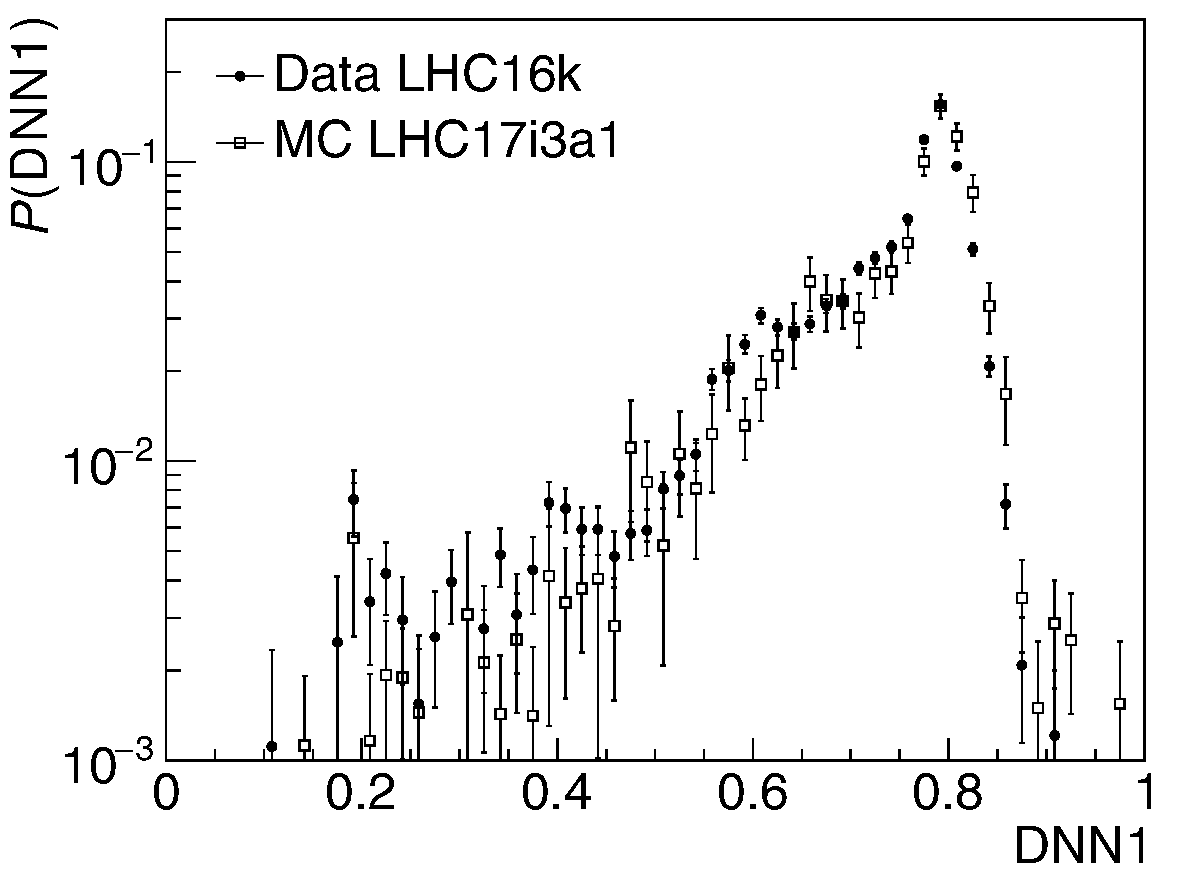
\includegraphics[width=0.3333\textwidth]{eta_dnn_08_12}%
%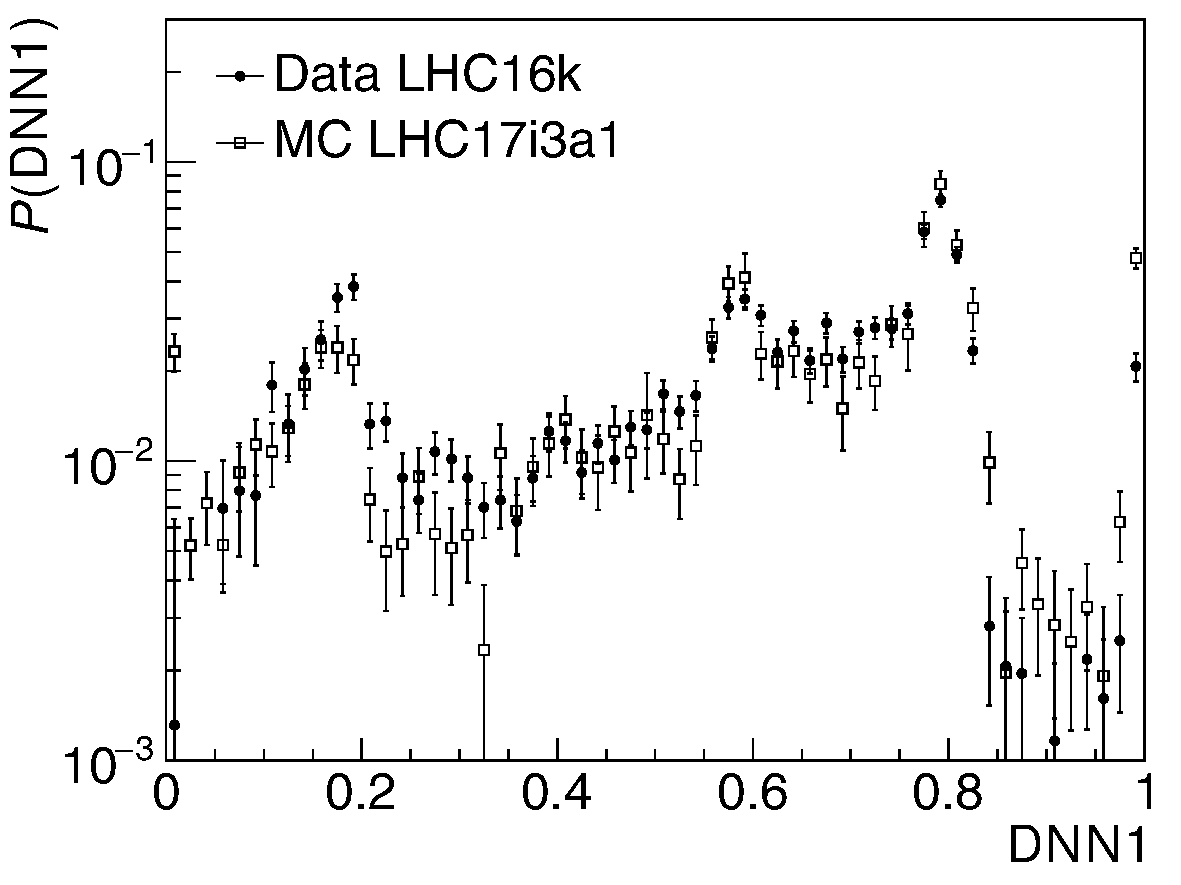
\includegraphics[width=0.3333\textwidth]{eta_dnn_12_20}%
%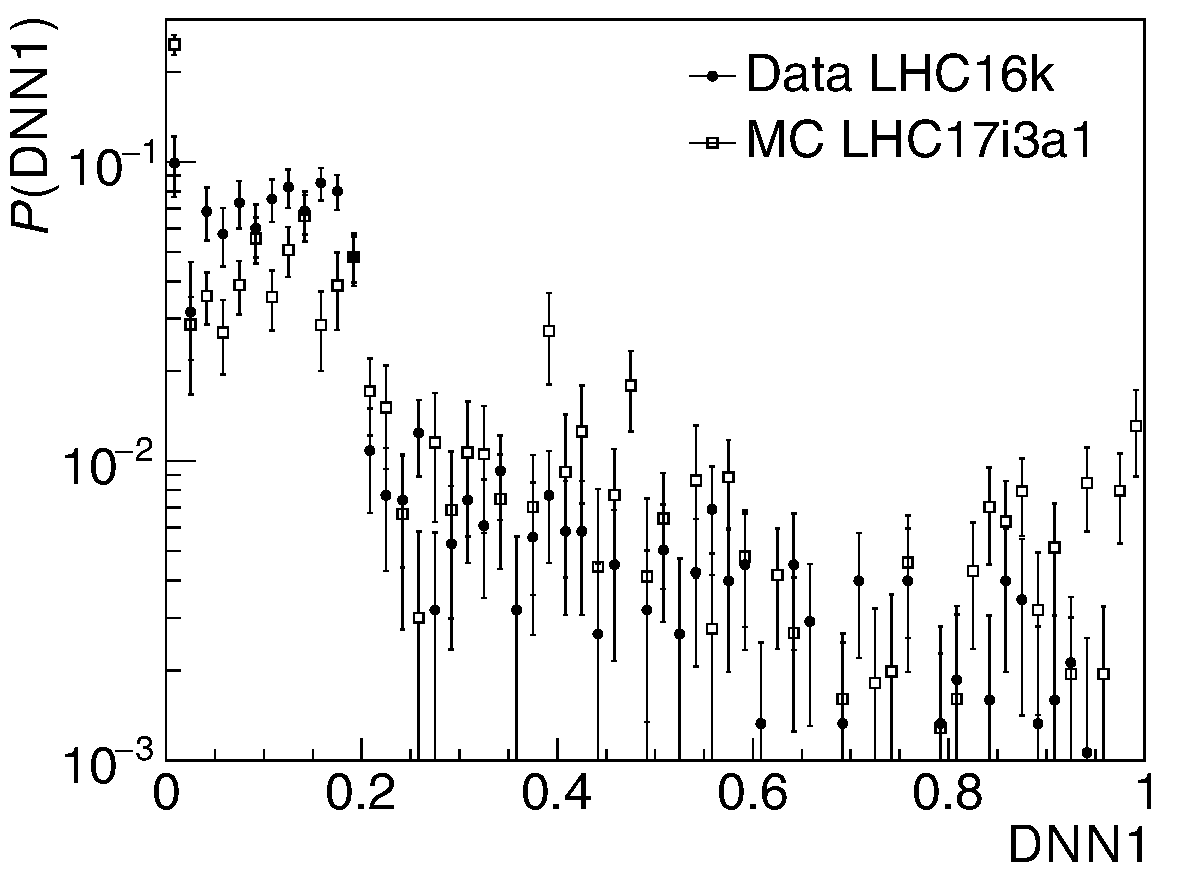
\includegraphics[width=0.3333\textwidth]{eta_dnn_20_30}}
%\centerline{\hfill$8 \le E_\gamma < 12\:\mathrm{GeV}$\hfill\hfill$12 \le E_\gamma < 20\:\mathrm{GeV}$\hfill\hfill$20 \le E_\gamma < 30\:\mathrm{GeV}$\hfill}
%\centerline{\hfill$\chi^2/\text{DOF} = 3.00$\hfill\hfill$\chi^2/\text{DOF} = 2.82$\hfill\hfill$\chi^2/\text{DOF} = 2.68 $\hfill}
%\caption{DNN activation for single photons, using $\eta \rightarrow \gamma\gamma$, comparing LHC16k with LHC17i3a1 MC. Note that for progressively higher energy photons, cluster merging occurs, and the activation starts to resemble $\pi^0 \rightarrow \gamma\gamma$ at lower energies.}
%\label{fig:eta_dnn}
%\end{figure}

%\begin{figure}[th]
%\centerline{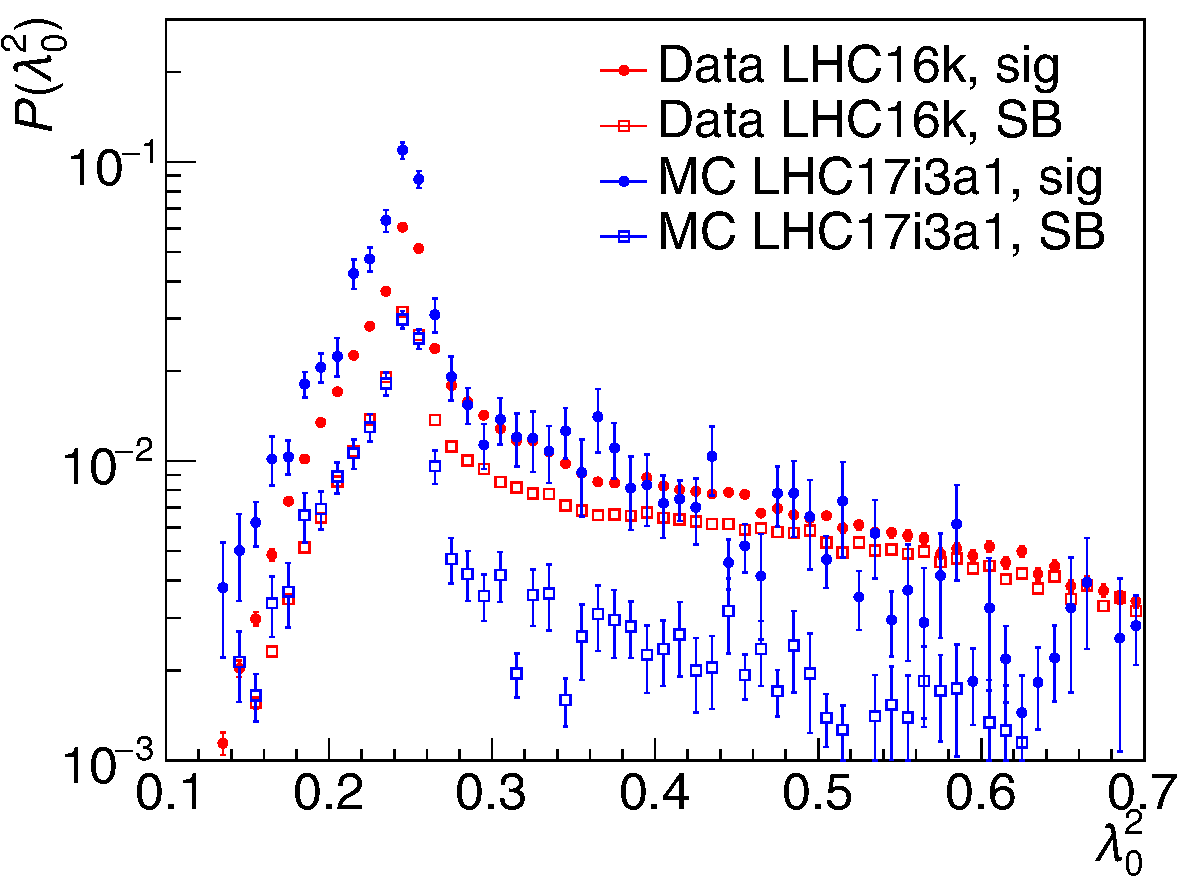
\includegraphics[width=0.5\textwidth]{eta_lambda02_08_12_sb}%
%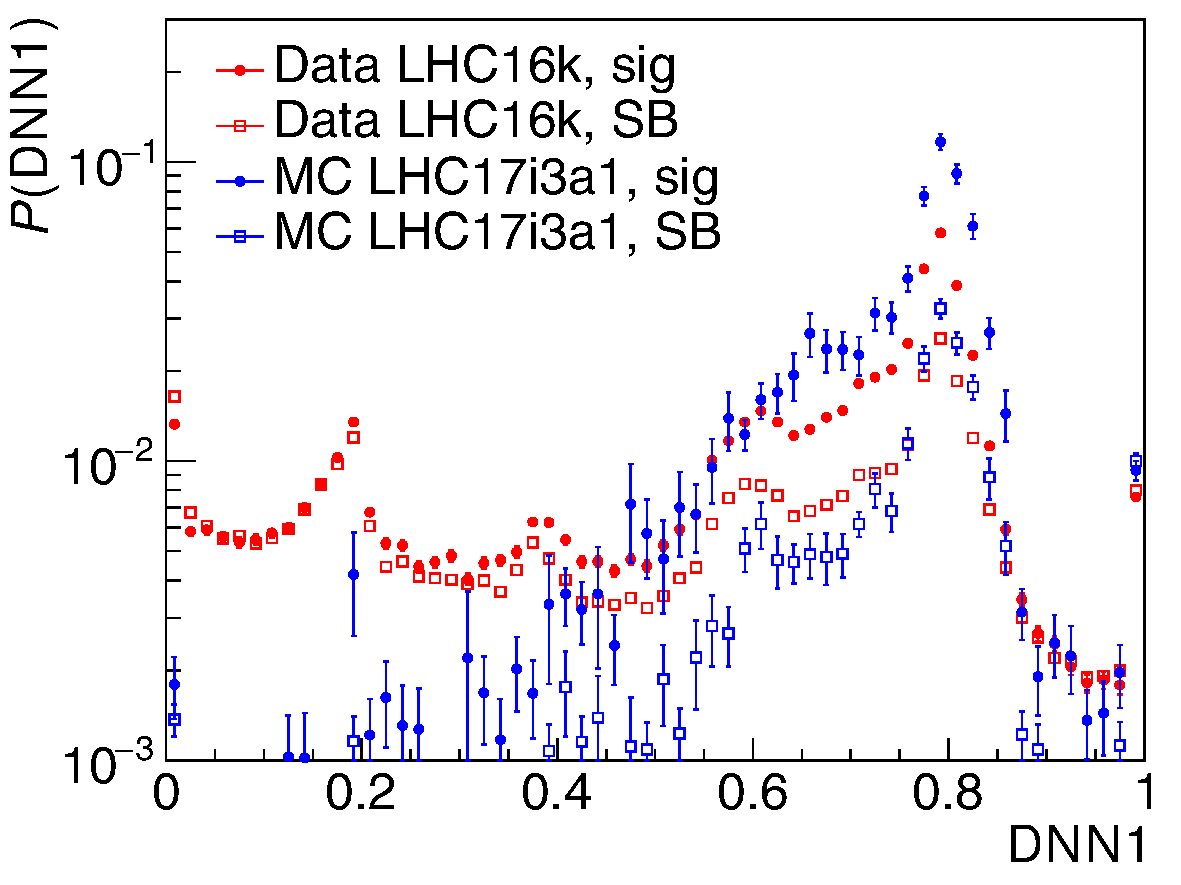
\includegraphics[width=0.5\textwidth]{eta_dnn_08_12_sb}}
%\caption{The $\lambda_0^2$ shower shape and DNN activation for the $\eta \rightarrow %\gamma\gamma$ signal and side-band region, comparing LHC16k with LHC17i3a1 MC.}
%\label{fig:eta_sb}
%\end{figure}

%In Fig.~\ref{fig:eta_lambda02}, the data/MC comparison is shown for the $\lambdasquare$ variable, where due to the weak shape dependence on single vs.\ two photons, the evolution from split to merged clusters is gradual.

%In Fig.~\ref{fig:eta_dnn}, the data/MC comparison is shown for the single photon DNN activation. A slight disagreement is visible at $0.8 < \mathrm{DNN1} < 0.9$, where the upper edge of the single photon peak falls slightly more steeply in data than in the MC. There is also slight disagreement between 0.26 and 0.3 in the $\lambdasquare$ variable for the same photon energy range, but it appears to be somewhat less pronounced.

%In Fig.~\ref{fig:eta_sb}, the data/MC comparison is shown for the $\lambdasquare$ and DNN variables separated for signal and side-band region. Since the MC does not reproduce all the physics processes in the data, the disagreement without side-band subtraction is expected.

%Some disagreement can be expected to arise due to the cross talk, which bleeds a small amount of the signal into neighboring electronics channels. However, we 
%bvj can unequivocally conclude 
%are convinced that the signal modeled by the MC is truly a single photon peak. Aside from this small bump, the region towards lower DNN1 is faithfully reproduced by MC.
%bvj , across 2 orders of magnitude. 
%This lends confidence that the region populated by both signal and background, where the template fitting is sensitive to the signal shape, is not affected by MC mismodelling. With increased $E_\gamma$, behavior analogous to $\pi^0 \rightarrow \gamma\gamma$ at lower $E_\gamma$ can be seen, where the diphoton clusters become merged.

%\subsection{Correlations and images}
%Figure~\ref{CorrelationLambdaDNN} shows the correlation between $\lambdasquare$ and neural network output, DNN, for clusters with {14$<\pt<$15 \GeVc} in p-Pb data that pass the selection described in Section~\ref{sec:clusterselection} including the isolation cut.  

%The sharp peak in $\lambdasquare$ is strongly correlated with the peak at DNN$\approx 0.75$, and the tail/bump structure in $\lambdasquare$ is correlated with the peak at DNN$\approx 0.2$. This shows that if these variables were used for binary classification, suitable cuts on both variables would largely agree. For example, about 70$\%$ of the clusters with {$\lambdasquare<0.4$} also have {DNN$>0.55$}, whereas 80$\%$ of the clusters with DNN$>0.55$ also have {$\lambdasquare<0.4$}.

%\begin{figure}[h]
%\center
%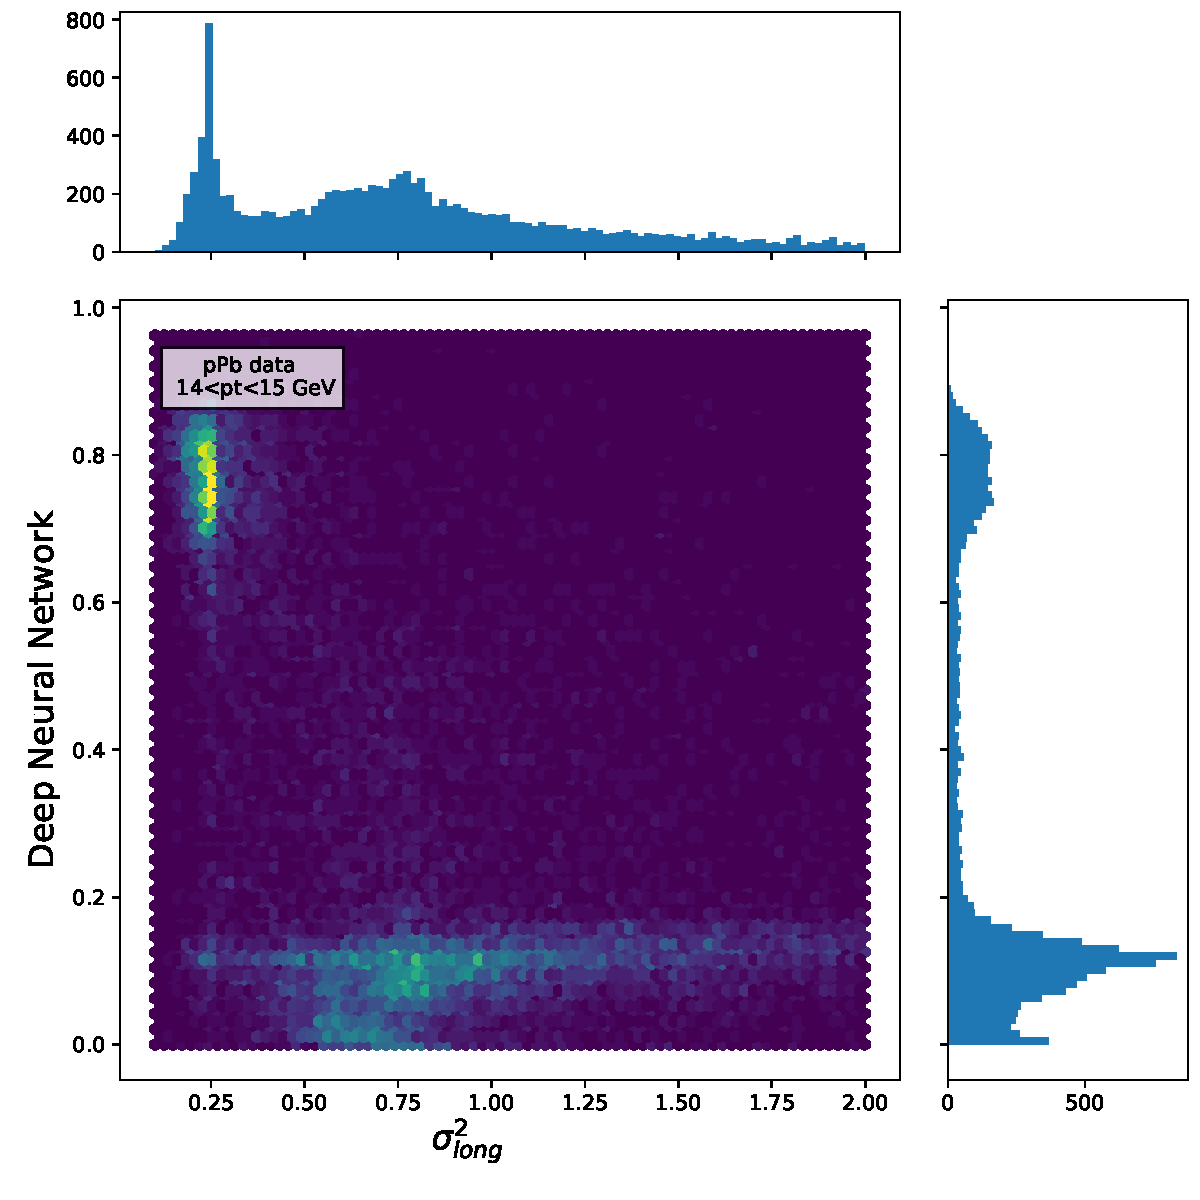
\includegraphics[width=0.495\textwidth]{PhotonID/Lambda_NN1_correlation}
%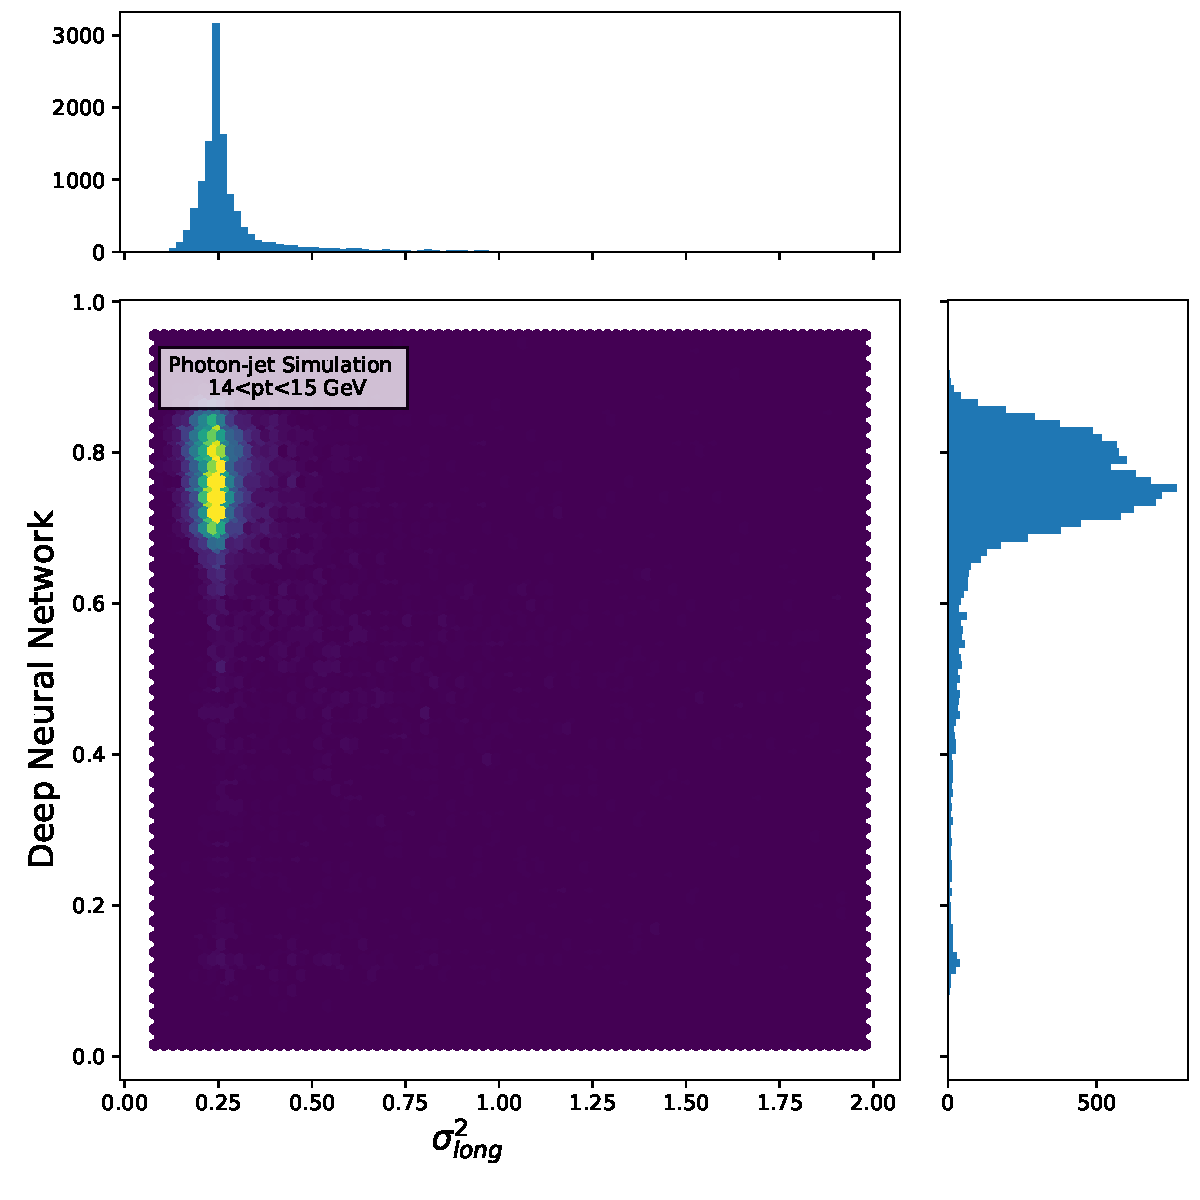
\includegraphics[width=0.495\textwidth]{PhotonID/Photon-jet_simulation_DNN_lambda}
%\caption{Correlation between $\lambdasquare$ variable and neural network for clusters within the range {14--15 \GeVc} in p-Pb data (left) and photon+jet simulation (right). The color code range is truncated for better visibility of the features of the data.}
%\label{CorrelationLambdaDNN}
%\end{figure}

%However, in this analysis we do not use these shower-shape variables for binary classification. Instead, we perform a shape analysis to extract our purity with the template fit method, as shown in Section~\ref{sec:purity}. Therefore, the use of these two variables, which have very different distributions, is not redundant.

% Figure~\ref{CorrelationDNNE} shows the correlation between DNN and the ratio of the energy in the leading cell to the total cluster energy $\emax$, which represents a rudimentary shower-shape variable. The correlation shows that low values of neural network select mostly clusters with $\emax$ in the range around 0.5, which are likely the product of symmetric $\pi^{0}\to\gamma\gamma$ decays. On the other hand, the large values of neural-network output corresponds to clusters with large values of $\emax$. Quantitatively, about 70$\%$ of the clusters with {$\emax>0.7$} also have {DNN$>0.55$}, whereas 80$\%$ of the clusters with DNN$>0.55$ also have $\emax<0.3$.

% \begin{figure}[h]
% \center 
% \includegraphics[width=0.495\textwidth]
% {PhotonID/DNN_emax_over_e_correlation}
% 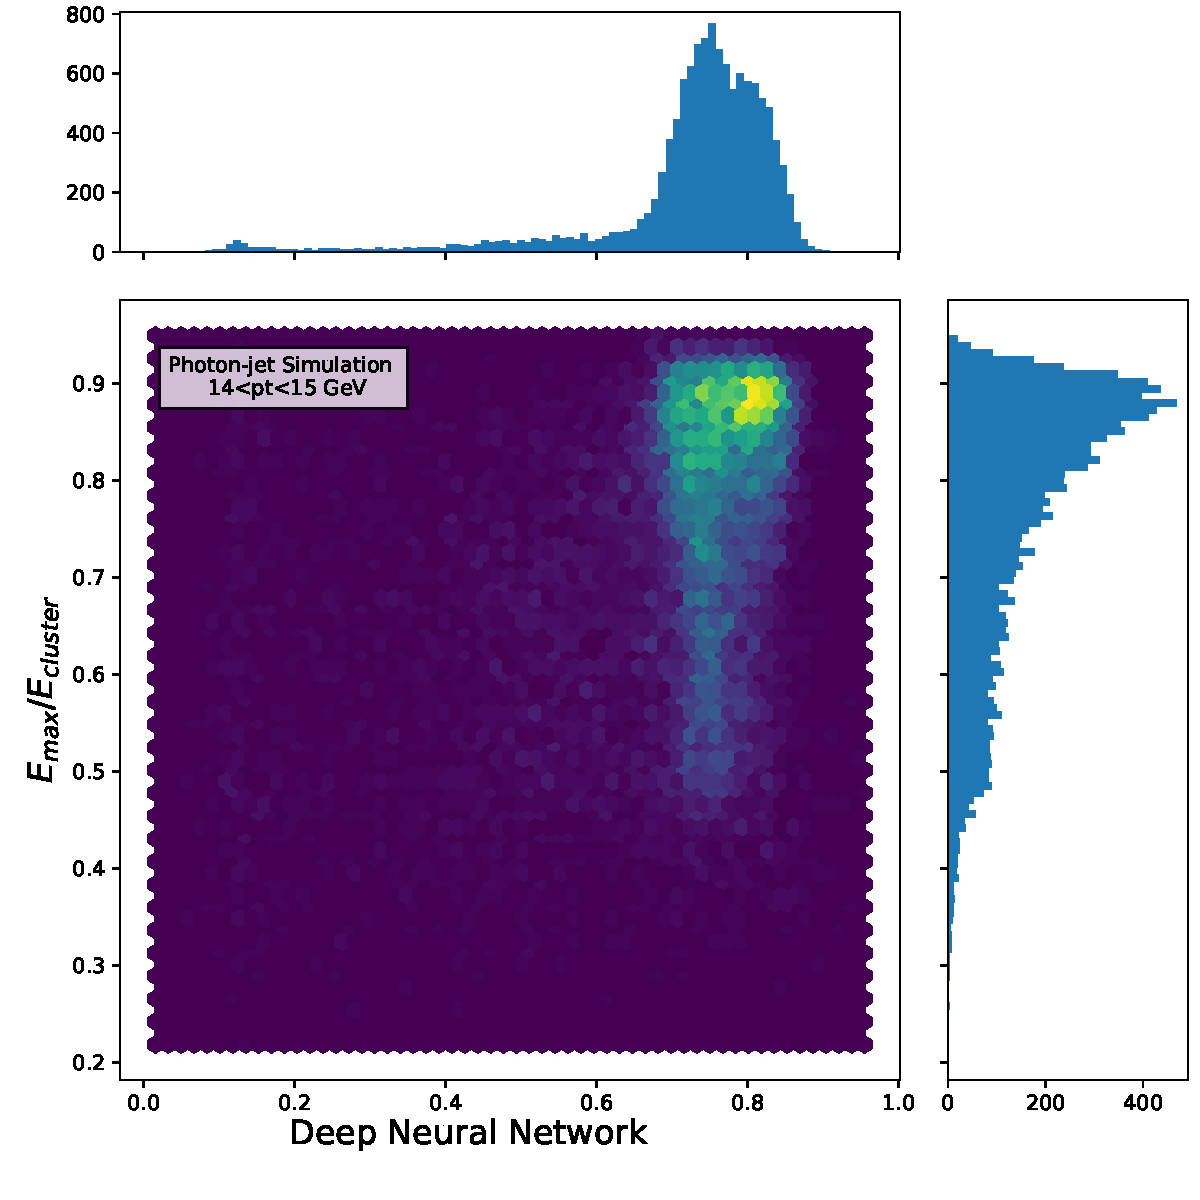
\includegraphics[width=0.495\textwidth]{PhotonID/Photon-jet_simulation_emax_over_ecluster_DNN}
% \caption{Correlation between $\emax$ variable and neural network output for clusters within the range {14--15 \GeVc} in p-Pb data (left) and photon+jet simulation (right).}
% \label{CorrelationDNNE}
% \end{figure}

%Figure~\ref{ClusterImages} shows a random selection of cluster shower shapes for clusters with {12$<\pt<$16 \GeVc} in pp data. The shower shapes are sorted by their DNN score, but the corresponding $\lambdasquare$ value is also shown for comparison. The clusters with DNN$>0.55$ are labeled as green, whereas the ones with DNN$<0.3$ are labeled with red. The clusters with DNN$>0.55$ deposit most of their energy (around 80$\%$ or more) in a single cell in most cases; this is the expected shower shape for photons as the cell dimensions are designed to be similar to the Moliere radius. On the other hand, the clusters with DNN$<0.3$ selection are much larger, have a more irregular shape, and often contain two maxima with similar strength, which is what we expect from $\pi^{0}$ decays that yield two showers that are not fully merged in a single cell.

%\begin{sidewaysfigure}
%\center
%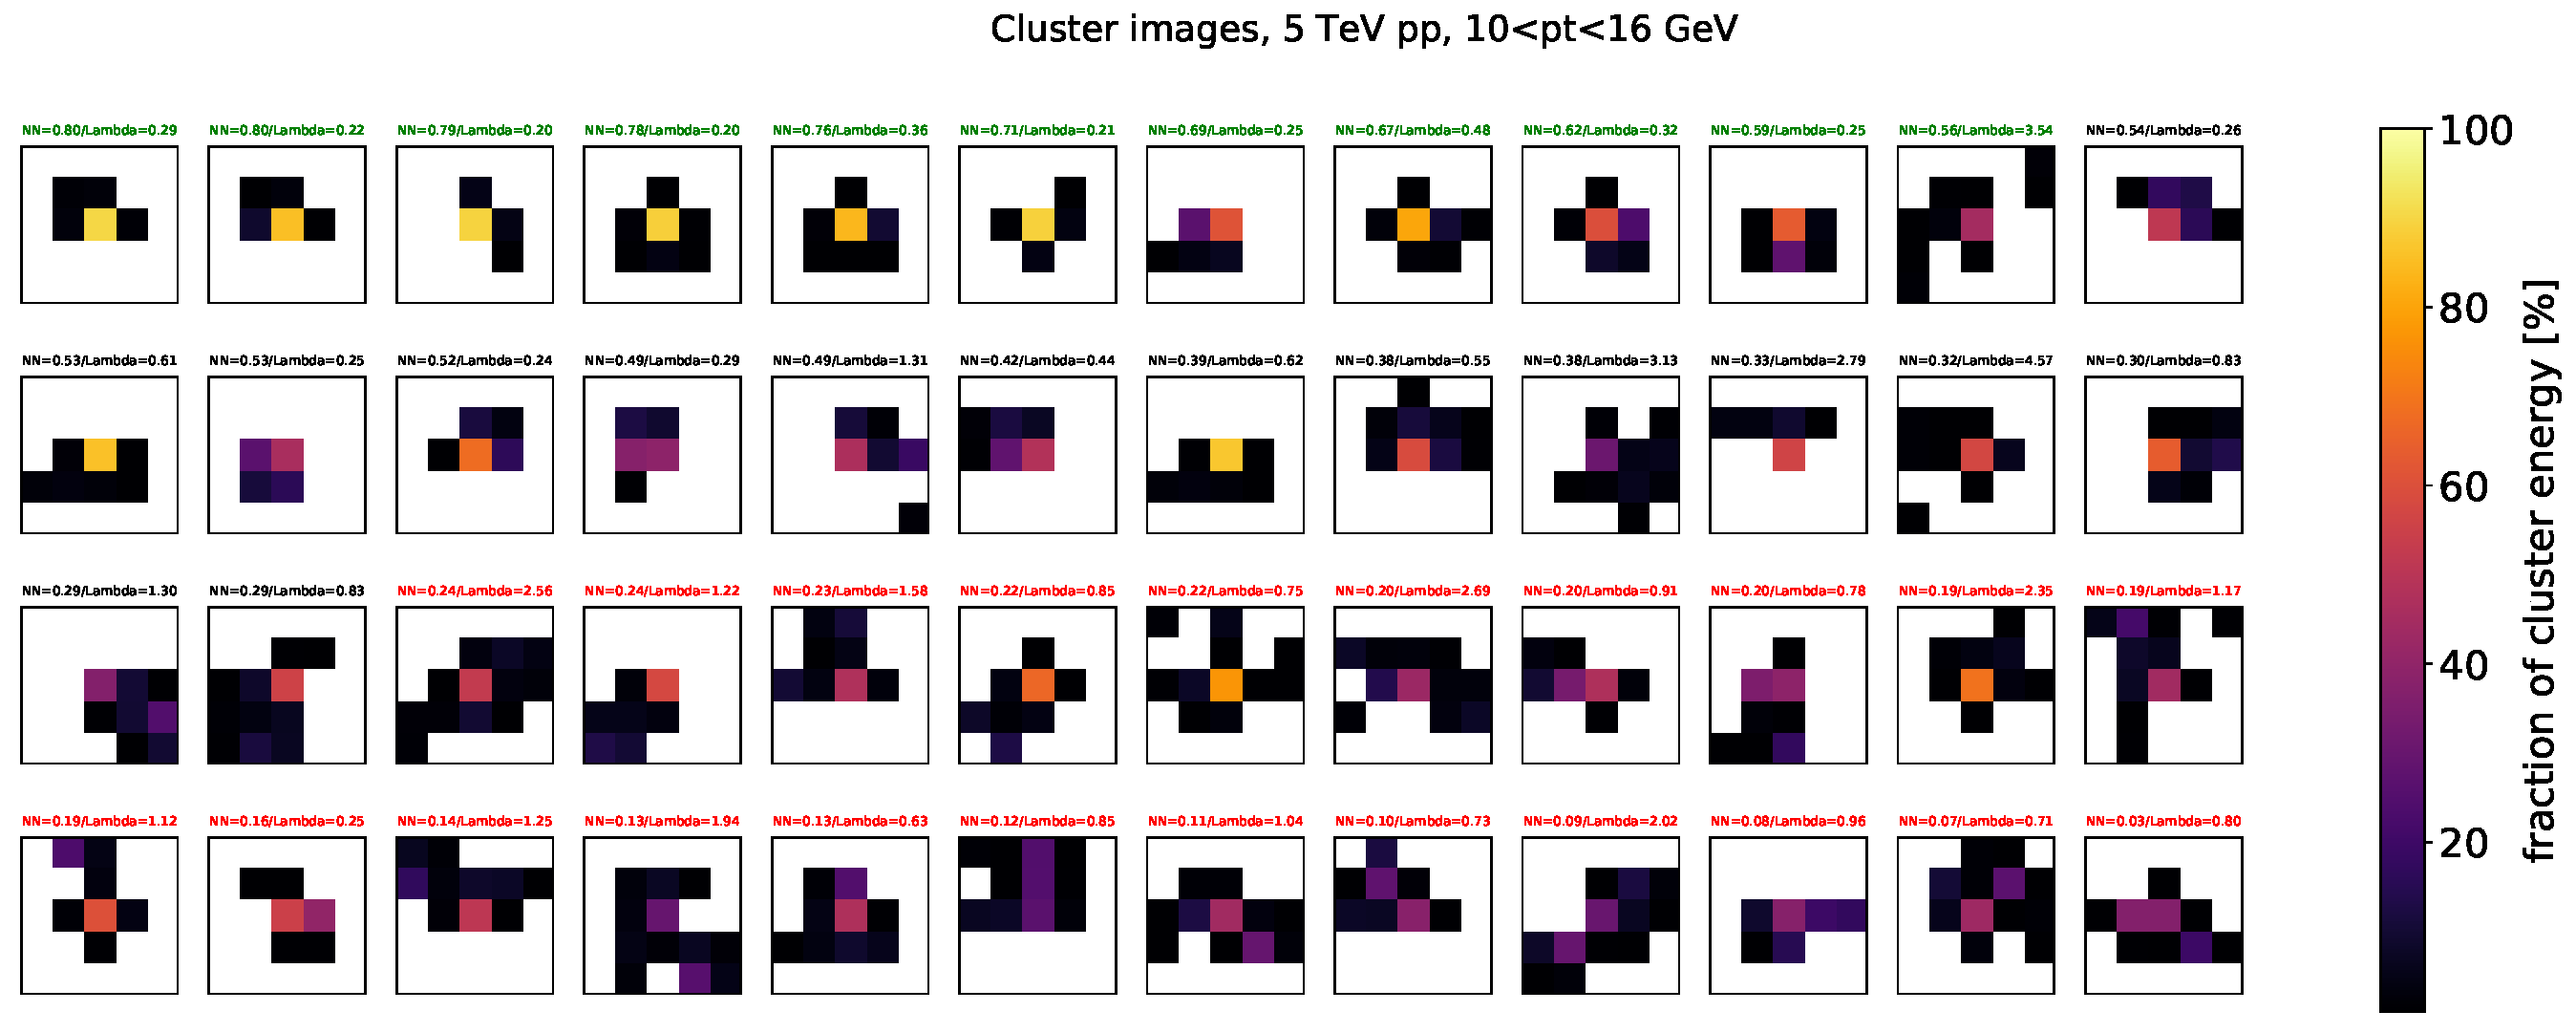
\includegraphics[width=1.0\textwidth]{PhotonID/ClusterImagesExample}
%\caption{Random selection of cluster shower-shape images of pp 5 TeV data for clusters that pass our selection. The color code represents the fraction of the total cluster energy that is within a given cell. Only cells around a matrix of 5$\times$5 cells around the seed cell of the cluster are shown. The images are sorted according to the output of the neural network from the upper left to the bottom right; the corresponding $\lambdasquare$ variable is also shown for each image. The title of the images passing our photon selection are shown in green, whereas the ones of the images passing our $\pi^{0}$ selection are shown in red.}
%\label{ClusterImages}
%\end{sidewaysfigure}

\FloatBarrier

\section{Isolation}
\label{sec:isolation}
In leading-order perturbative calculations, prompt photons are produced surrounded by small hadronic activity and fragmentation photons are only found within a jet. Beyond leading order, the direct and fragmentation components have no physical meaning and cannot be factorized; the sum of their cross sections is the physical observable. However, theoretical calculations can be simplified through the use of an isolation requirement, which also suppresses the background from decays of neutral mesons.

We construct an isolation variable using only tracking information and avoid using calorimeter clusters. This choice prevents biases due to the correlation between 
isolation criteria and $\pi^{0}$ decay opening angle and allow us to use the full acceptance of EMCal. This is at the expense of a lower purity.

The isolation variable for this analysis is defined as the scalar sum of the transverse momentum of charged particles within an angular radius around the cluster direction, $R =\sqrt{(\Delta\varphi)^{2} +(\Delta\eta)^{2}  } =0.4$ (with $\Delta\varphi$ measured in radians), thus:
\begin{equation}
\iso^{\mathrm{raw}} = \sum_{\mathrm{track}~\in~\Delta R < 0.4}  \pt^{\mathrm{track}}   
\label{eq:isoraw}
\end{equation}
The charged particles used as input for the isolation calculation have {$0.15<\pt<10$ \GeVc}, {$|\eta|<0.8$} and pass the selection described in Section~\ref{sec:tracking}. 

The isolation variable defined in Equation~\ref{eq:isoraw} is susceptible to background from the charged particles from the underlying event, e.g. a truly isolated photon might appear non isolated due to overlap with particles not associated with the hard scattering. In order to correct for this effect, we apply an event-by-event underlying event subtraction, which is described in the following section. 

\subsection{Underlying Event estimation}
\label{sec:UEsubtraction}
In this section, we describe how we estimate and subtract the ``underlying event'' (UE). The UE is defined as the particles not associated with the hard-scattering of the collision\footnote{In Ref.~\cite{ALICE:2011ac}, the UE is defined as ``the sum of all the processes that build up the final hadronic state in a collisions excluding the hardest leading order partonic interaction. This includes fragmentation of beam remnants, multi-parton interactions and initial and final-state radiation associated with each interaction."}. We subtract the UE from the measured transverse momentum of jets and in the photon isolation (described in Section~\ref{sec:isolation}). 
Technically, the discrimination between the soft component from the hard component of an event is performed using the \textsc{Fastjet} jet area/median method~\cite{Cacciari:2009dp}, which uses the median of the distribution of transverse momentum densities of all jets in an event. We use one of the standard jet areas definition implemented in \textsc{FastJet} called Voronoi area~\footnote{The method used is the following fastjet::VoronoiAreaSpec \url{http://www.fastjet.fr/repo/doxygen-2.4.5/classfastjet_1_1VoronoiAreaSpec.html} }.

The estimation of the UE density uses jets $J'$ reconstructed by the
$k_{\mathrm{T}}$-algorithm\footnote{In contrast to the anti-$k_{\mathrm{T}}$ algorithm, the $k_{\mathrm{T}}$ algorithm clusters the softest particles first, and thus is more sensitive to the details of the distribution of softer objects and better suited for an investigation of the underlying event.} with distance parameter $R=0.3$. The estimated UE
density is defined as:
\begin{equation}
  \rho = \mathrm{med} \left\{ \frac{\sum_{i\in J'_k}
    p_{T,i}}{\sum_{i\in J'_k} A_i} \right\}
\end{equation}
where $p_{T,i}$ is the transverse momentum, and $A_i$ the Voronoi area
of the particle $i$ within the jet reconstructed for UE estimation
purpose $J'_k$. Following standard practice, the two leading jets are not considered in this observable, to limit the contribution from the hard component of the interaction. 

The choice of the median is motivated by its robustness against outliers, which includes jets originated by hard interactions. The observable
thus isolates UE  by assuming that most of the event is either empty or dominated by soft contributions and that the hard component of the interaction is well contained within the leading jets~\citep{Cacciari:2009dp}. 

Figure~\ref{fig:Rho} shows the median charged-particle density, $\rho$, distribution obtained in pp and p-Pb data in minimum bias events and in events that pass the selection in Section~\ref{sec:eventselection} and thus have a high-$\pt$ cluster. The distribution in minimum-bias events decreases approximately exponentially. The distribution in photon-triggered events is different and follows sort of an asymmetric Gaussian distribution that peaks at approximately {1.0 \GeVc} and {2.5 \GeVc} for pp and \pPb~collisions, respectively. 
\begin{figure}
\center
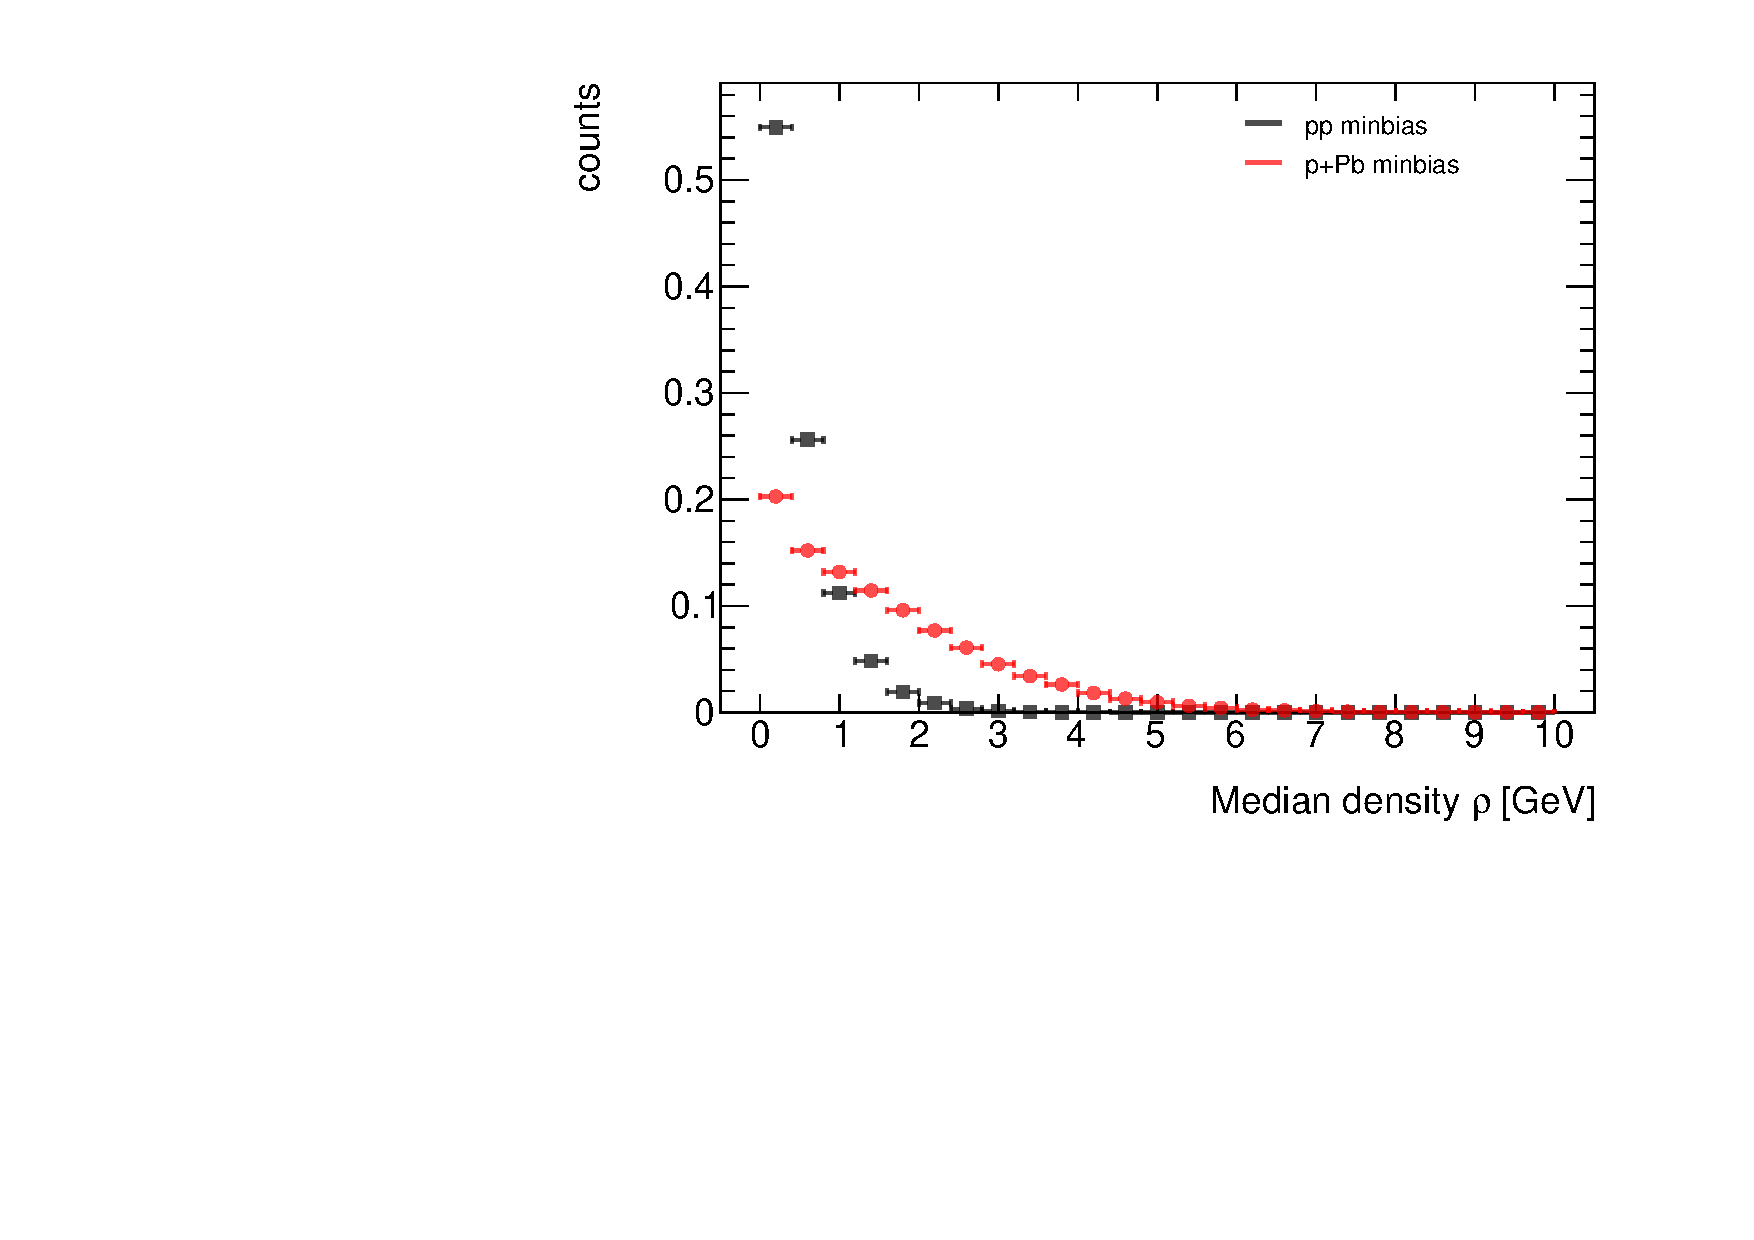
\includegraphics[width=0.49\textwidth]{UE/Rho_MinBias}
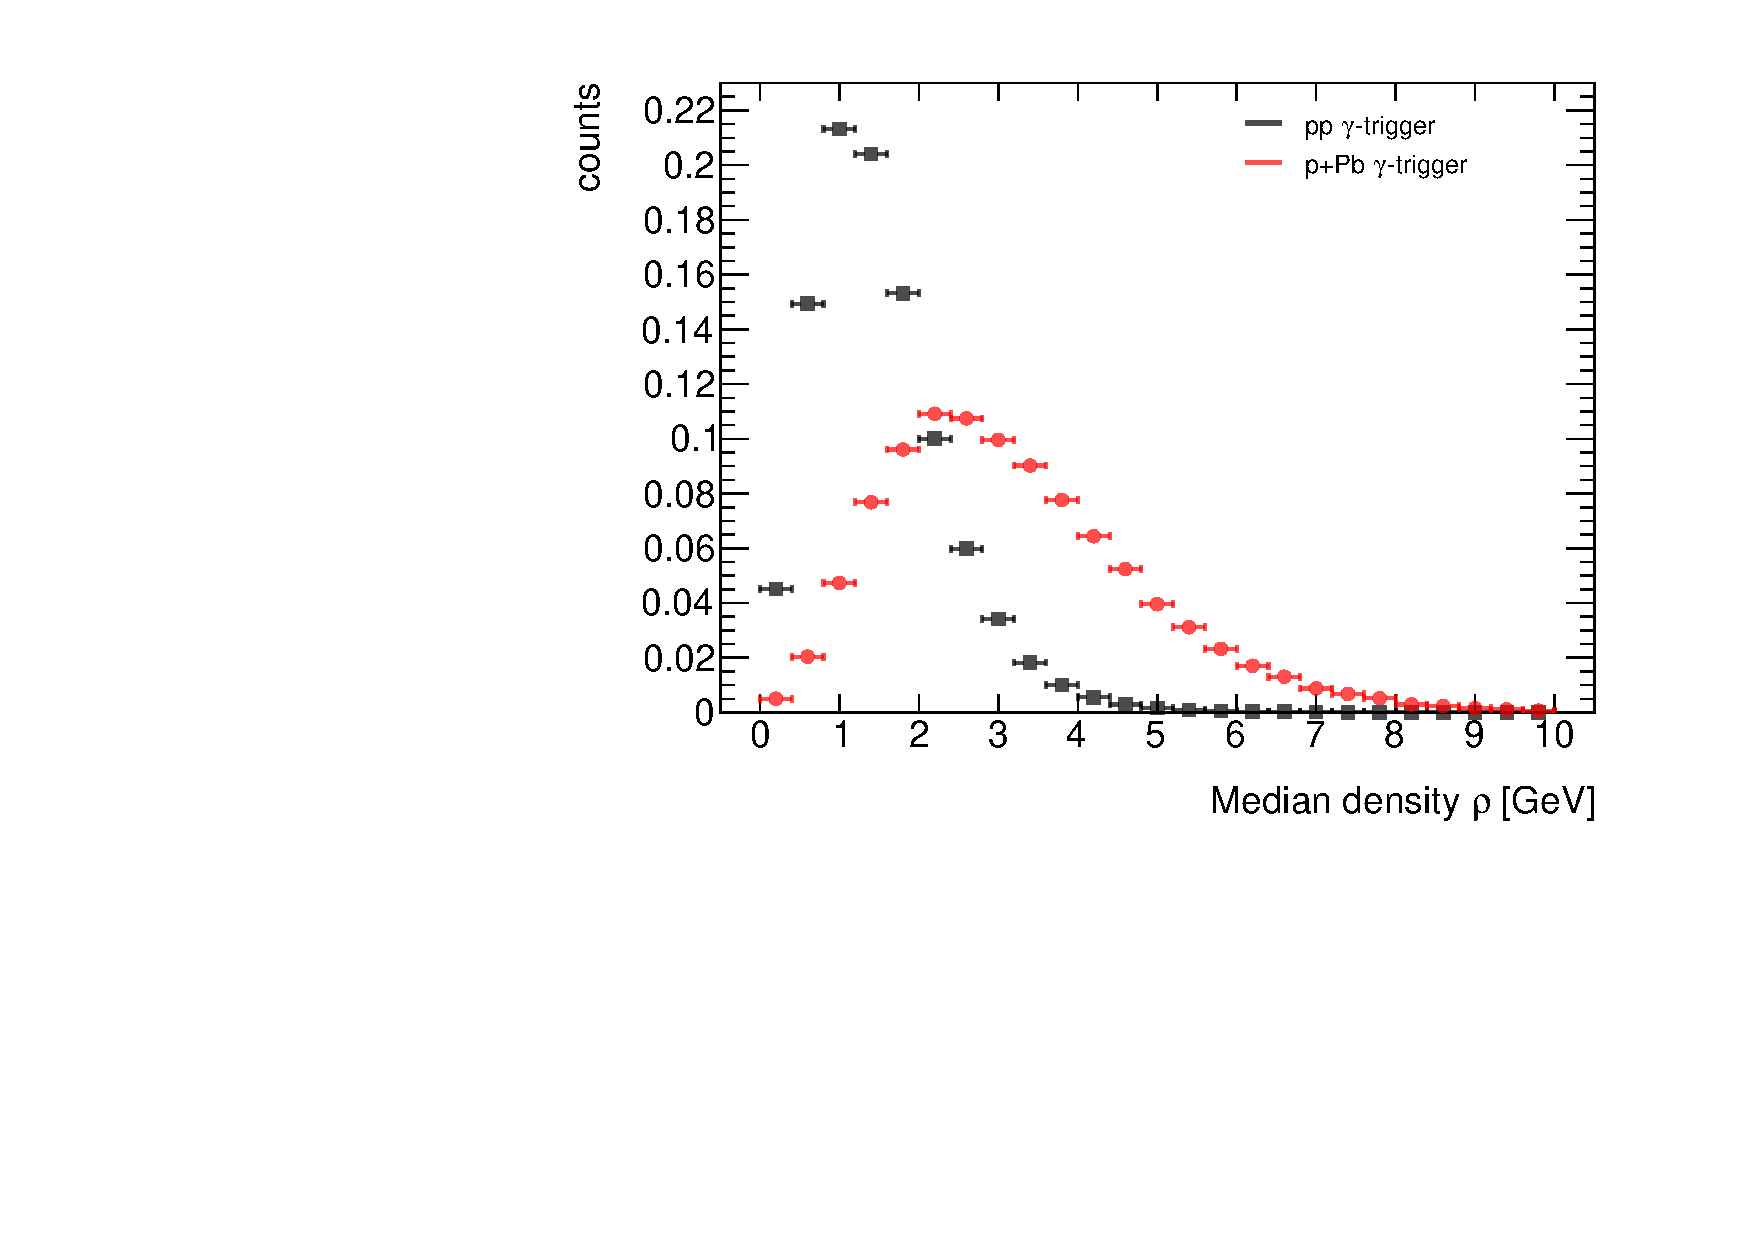
\includegraphics[width=0.49\textwidth]{UE/Rho_GammaTrigger}
\caption{Distribution of the median charged-particle transverse momentum density, $\rho$, in pp and \pPb~data, for a minimum-bias selection (left panel) and in photon-triggered events (right panel). }
\label{fig:Rho}
\end{figure}

The mean and standard deviation for each distribution is shown in Table~\ref{tab:rhoestimates}. The difference in UE-density in \pPb~is expected due to the increased number of nucleon-nucleon collisions. The UE-densities shown here are still about a factor of 50 lower than in central Pb-Pb collisions.
\begin{table}[h]
   \centering
   \caption{Median transverse momentum density mean and standard deviation in minimum-bias and and photon-triggered events in pp and \pPb~data. The statistical uncertainty in these numbers is negligible.}
   \label{tab:rhoestimates}
   \begin{tabular*}{1.0\columnwidth}{@{\extracolsep{\fill}}lcc|cc@{}}
    \hline
     &  pp minbias & pp $\gamma-$trigger & \pPb~ minbias & \pPb~$\gamma$-trigger  \\
       \hline
       $\langle\rho\rangle$   & 0.49 \GeVc & 1.51 \GeVc & 1.56 \GeVc & 3.19 \GeVc \\ 
       $\sigma_{\rho}$       &  0.47 \GeVc &  0.85 \GeVc  & 1.32 \GeVc & 1.60 \GeVc \\ 
            \hline        
   \end{tabular*}
\end{table}

The average $\rho$ for photon-triggered events reported in Table~\ref{tab:rhoestimates} is consistent with an independent estimate, based on the ``$\eta$-band'' method, that uses the same dataset and cluster selection~\cite{Erwann}. 


%\subsubsection{UE subtraction for jet transverse momentum}
%In this section, we show the result of using the measured median density to estimate UE-background for jets. We perform a jet-by-jet subtraction event-by-event. The subtracted transverse momentum of a given jet is:
%\begin{equation}
%  p_{\mathrm{T, rec}} = p_{\mathrm{T,raw}} - \rho \times A. 
%    \label{eq:jetsubtraction}
%\end{equation}
%\FloatBarrier
%Here $p_{\mathrm{T, rec}}$ is the raw transverse momentum and $A$ is the jet area.

%This approach neglects the fact that the UE-density for a given event is not uniform in $\eta$-$\phi$ but fluctuates from region to region. These fluctuations are mainly Poissonian but also encode correlated region-to-region variations of the particle multiplicity and mean $\pt$. 

%We check the impact of the fluctuations on the UE-subtraction by using Equation~\ref{eq:jetsubtraction} to measure the jet transverse momentum distribution in minimum-bias events, where the contribution from jets from a hard scattering is minimal and the reconstructed jets arise mainly from the UE and its fluctuations. That is, ideally the $p_{\mathrm{T, rec}}$ distribution should be a very narrow distribution centered around zero. 

%igure~\ref{fig:JetUE} shows the UE-subtracted transverse momentum distribution of jets in minimum-bias events in pp and p-Pb data. Only jets with $|\eta|<0.5$ are shown. In both cases, the distribution is centered around zero (the mean of the distribution if {$-$0.08 \GeVc} for pp and {0.02 \GeVc} for p-Pb data), and falls rather rapidly to both sides (the standard deviation is {1.13 \GeVc} for pp and {1.35 \GeVc} for p-Pb data). This demonstrates that the UE-subtraction for jet reconstruction works as intended. 

%\begin{figure}
%	\center
%	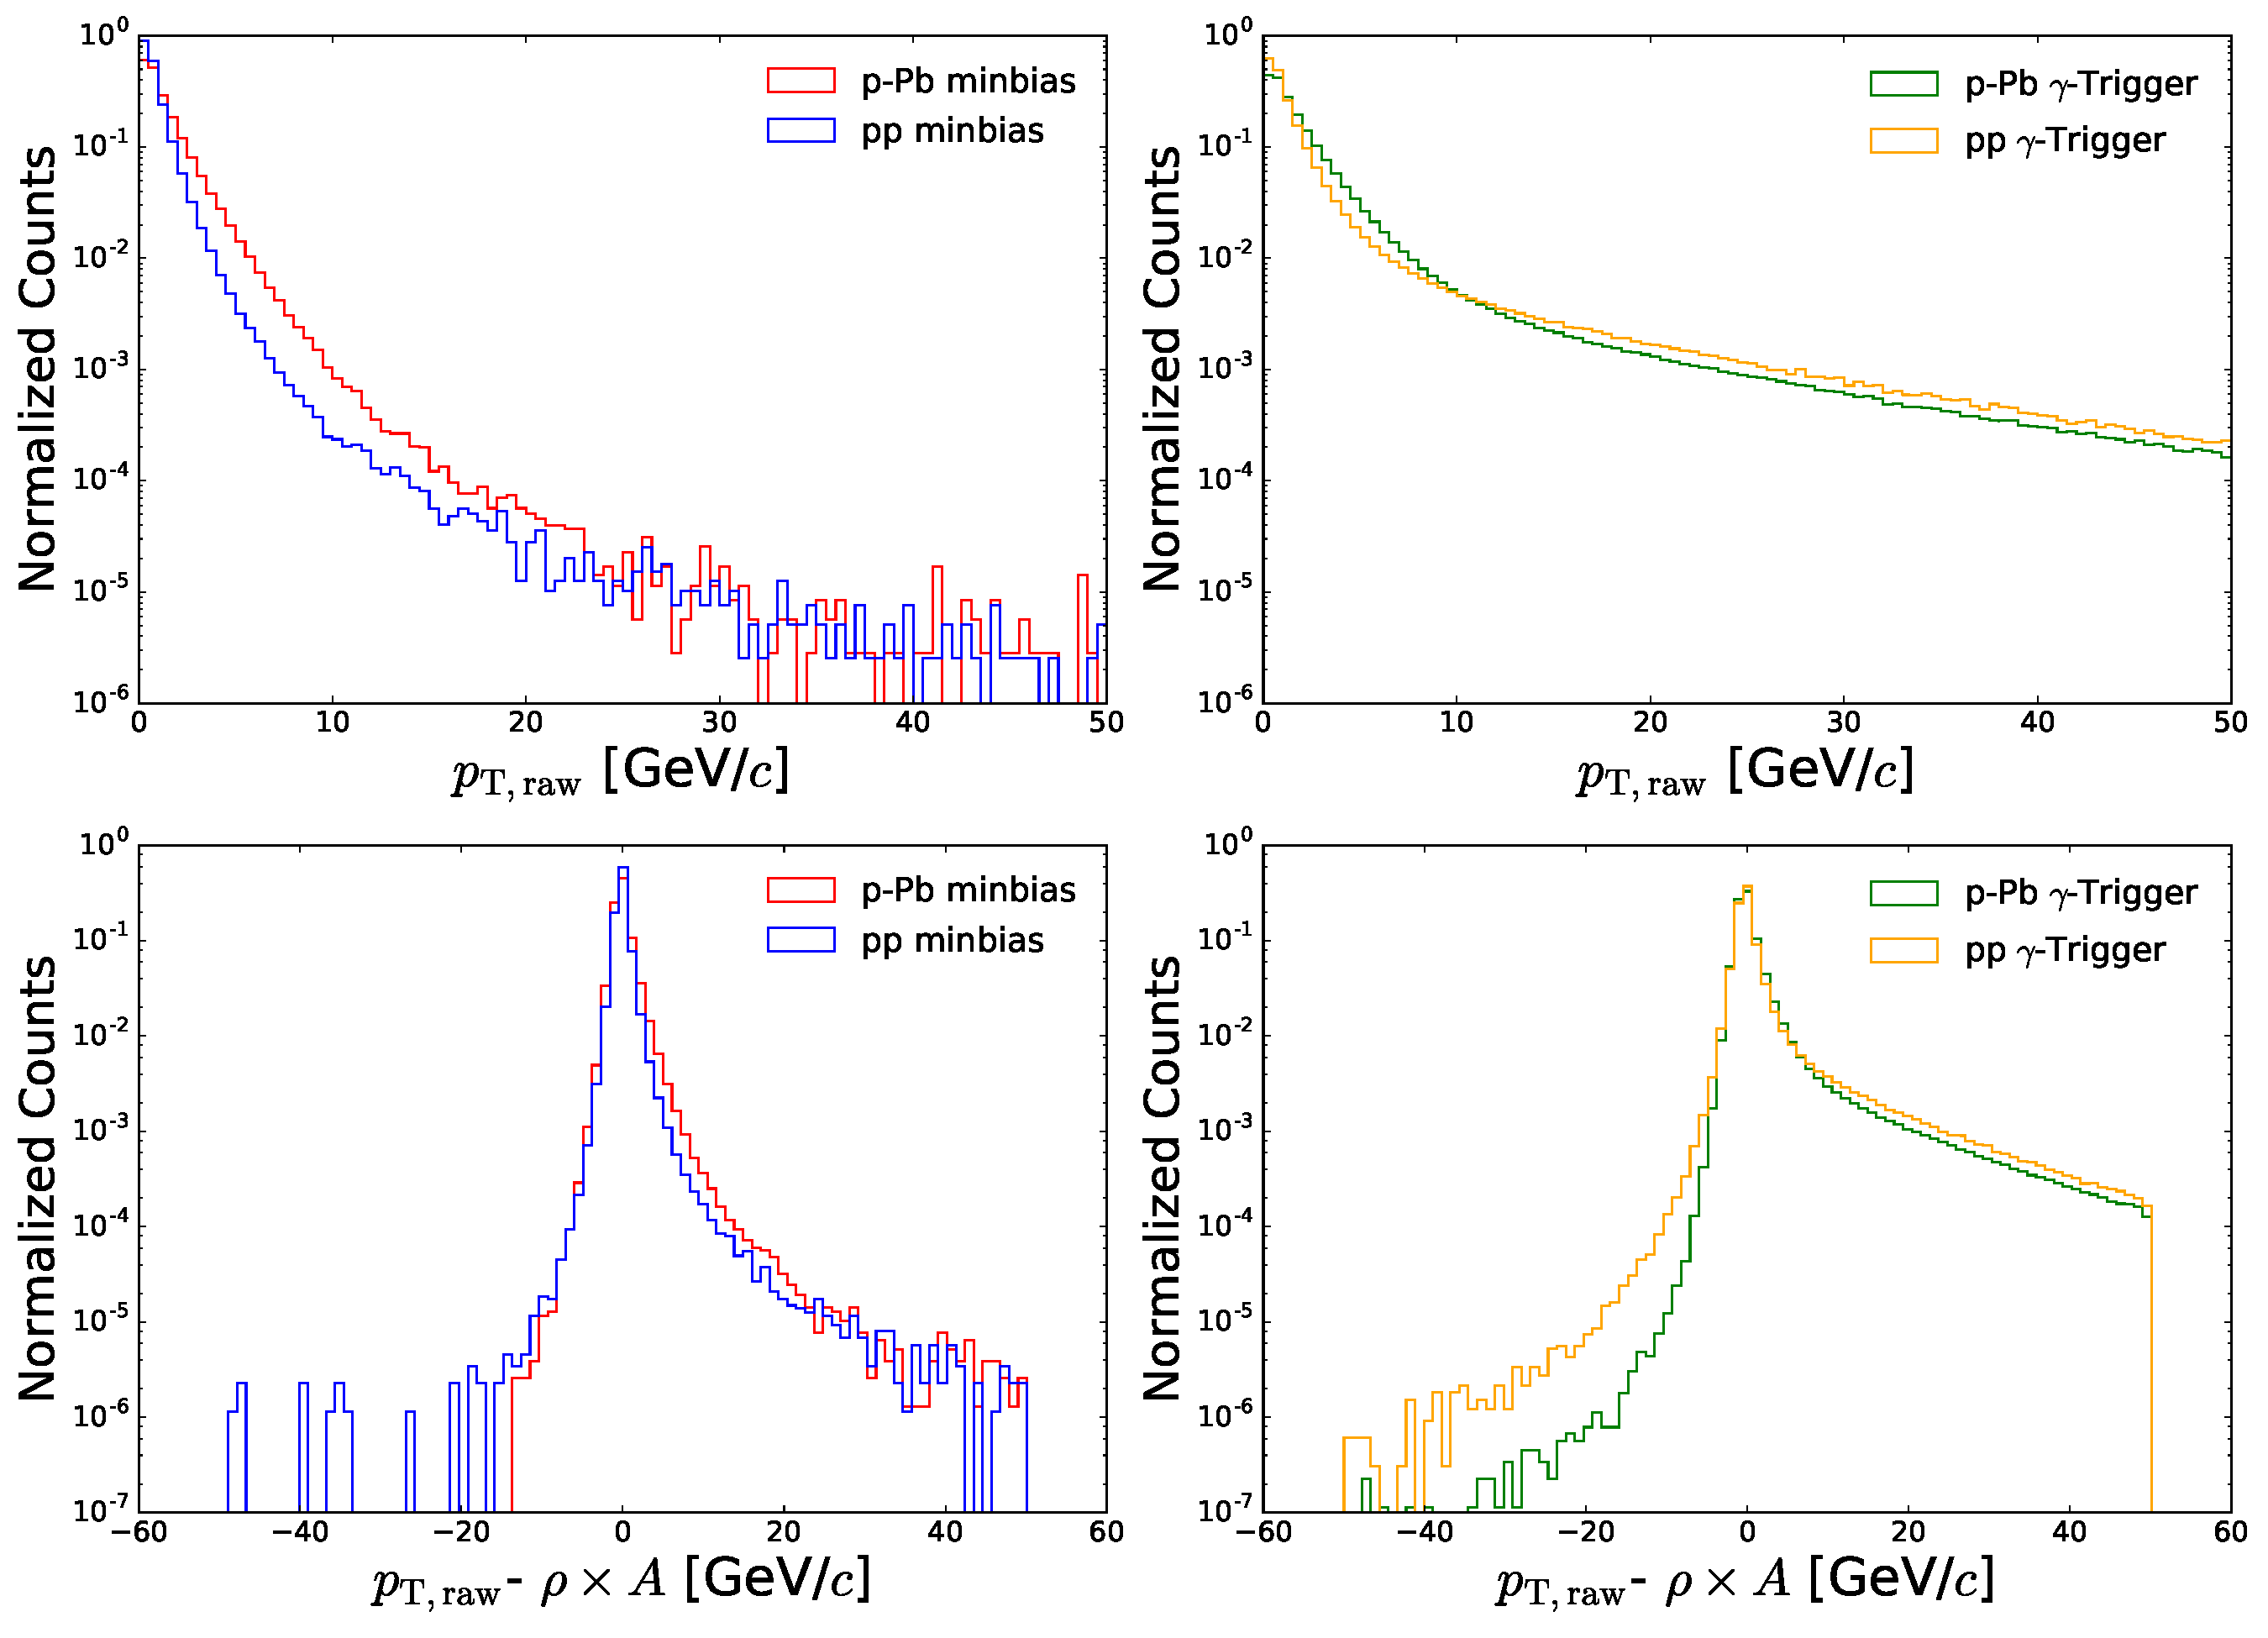
\includegraphics[width=0.9\textwidth]{UE/ppandpPb_jet_distributions.pdf}
%	\caption{A comparison between the jet transverse momentum distributions, both raw and  UE-subtracted, for minimum-bias and photon-triggered events in pp and p-Pb data. The raw jet transverse momentum distributions in minimum-bias events (upper left) and photon-triggered (upper right) in pp and p-Pb data are shown on the upper row. The UE-subtracted jet transverse momentum distributions in minimum-bias event (bottom left) and photon-triggered events (bottom right) in pp and p-Pb data are shown on the bottom row.}
%\label{fig:JetUE}
%\end{figure}

%The unphysical negative tail in Figure~\ref{fig:JetUE} arises due to UE over-subtraction. That is, the local UE density in the jet area is significantly lower than the calculated median density. On the other hand, the positive tail could be due to under-subtraction, however there are also a contribution from hard-scatterings in minimum-bias events, and there is a clear enhancement in photon-triggered events, as expected. 

%Table~\ref{TableUEUnderAndOverSubtraction} shows the fraction of jets shown in Figure~\ref{fig:JetUE} that satisfy a given threshold in subtracted  $p_{\mathrm{T, rec}}$. The results show that over-subtraction results in less than 0.5$\%$ of jets with $p_{\mathrm{T, rec}}<-3$ \GeVc. The fraction of jets with $p_{\mathrm{T, rec}}>5$ \GeVc~is less than a percent in minimum-bias p-Pb events, and drops to $0.13\%$ $p_{\mathrm{T, rec}}>10$ \GeVc. This informs our choice of minimum $p_{\mathrm{T, rec}}$ selection used for photon--jet analysis presented in Section~\ref{sec:GammaJet}. 

%\begin{table}[h]
%   \centering
%   \caption{Fraction of jets satisfying various UE-subtracted transverse momentum ranges in minimum bias events.}
%   \begin{tabular*}{1.0\columnwidth}{@{\extracolsep{\fill}}lccccc@{}}
%    \hline
%         &  pp minbias & p-Pb minbias  \\
%       \hline13

%       $p_{\mathrm{T,rec}}$ = $p_{\mathrm{T,raw}}$ - $\rho \times A$ $<$ $-$5.0 \GeVc & 0.05$\%$ & 0.05$\%$  \\ 
%       $p_{\mathrm{T,rec}}$ = $p_{\mathrm{T,raw}}$ - $\rho \times A$ $<$ $-$3.0 \GeVc & 0.32$\%$ & 0.46$\%$  \\
%       $p_{\mathrm{T,rec}}$ = $p_{\mathrm{T,raw}}$ - $\rho \times A$ $<$ $-$1.5 \GeVc & %3.24$\%$ & 5.28$\%$  \\
%       $p_{\mathrm{T,rec}}$ = $p_{\mathrm{T,raw}}$ - $\rho \times A$ $<\:\:\:\:\:\:\:\:\:\:\:$ 0 \GeVc & 63.52$\%$ & 61.55$\%$  \\
 %      \hline
 %      $p_{\mathrm{T,rec}}$ = $p_{\mathrm{T,raw}}$ - $\rho \times A$ $>\:\:\:$ 3.0 \GeVc & 1.02$\%$ & 2.73$\%$  \\
  %     $p_{\mathrm{T,rec}}$ = $p_{\mathrm{T,raw}}$ - $\rho \times A$ $>\:\:\:$ 5.0 \GeVc & 0.34$\%$ & 0.85$\%$  \\
 %      $p_{\mathrm{T,rec}}$ = $p_{\mathrm{T,raw}}$ - $\rho \times A$ $>\:\:\:$ 7.0 \GeVc & 0.16$\%$ & 0.34$\%$  \\
%       $p_{\mathrm{T,rec}}$ = $p_{\mathrm{T,raw}}$ - $\rho \times A$ $>$ 10.0 \GeVc & 0.08$\%$ & 0.13$\%$  \\
%    \hline
%%    \label{TableUEUnderAndOverSubtraction}
%	\end{tabular*}
%\end{table}

%Figure~\ref{fig:ppandpPb_mean_RhoA} shows the average UE energy that is subtracted on a jet-by-jet basis following Equation~\ref{eq:jetsubtraction}. There is a strong anti-correlation between the event $\rho$ and the jet area so while the density is a factor of 2 or so higher (as shown in Table~\ref{tab:rhoestimates}), the total average $\rho\times A$ is only about 20--30$\%$ higher in p-Pb collisions compared to pp collisions. 

%\begin{figure}[h]
%	\center
%	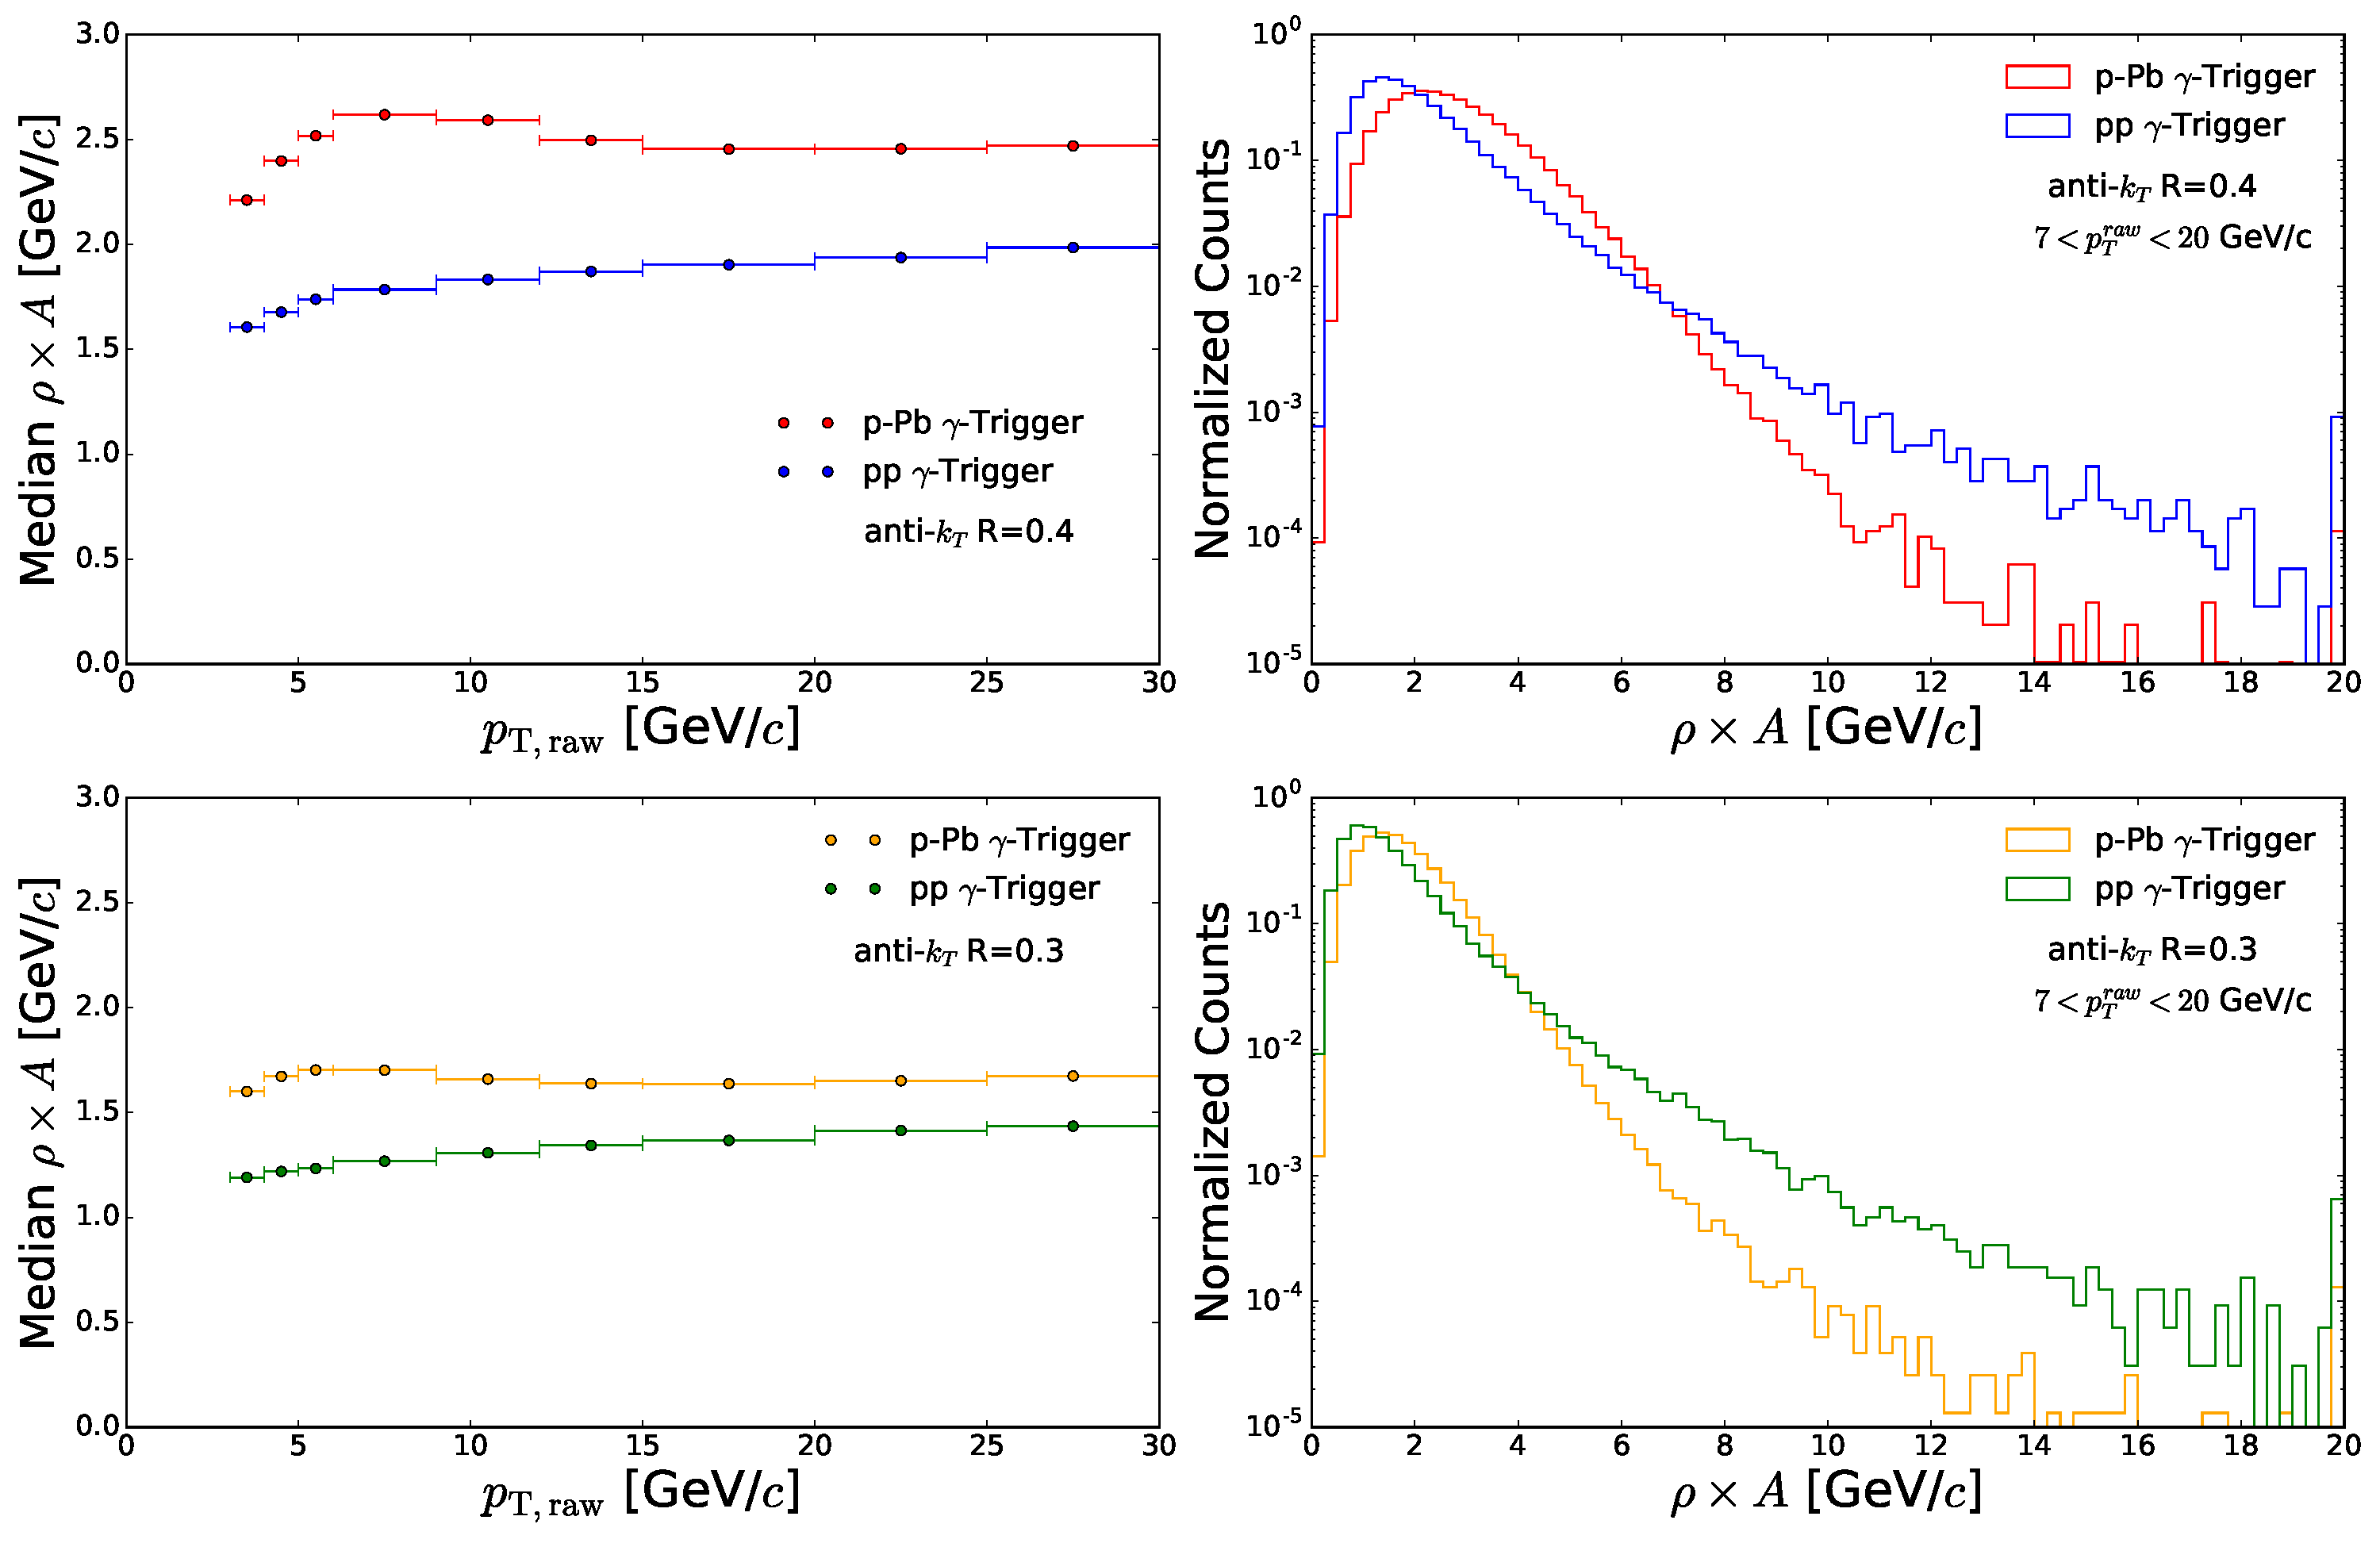
\includegraphics[width=0.99\textwidth]{JetReco/ppandpPb_median_AreaRho.pdf}
%	\caption{The average amount of UE-subtraction as a function of unsubtracted jet transverse momentum for photon-triggered events in pp and p-Pb data is shown on the left column for reconstructed jets of R = 0.3 and 0.4. The distribution of how much is UE-subtracted from jets with unsubtracted jet transverse momentum greater than {7 \GeVc} for photon-triggered events in pp and p-Pb data is shown on the right column for reconstructed jets of R = 0.3 and 0.4.}
%	\label{fig:ppandpPb_mean_RhoA}
%\end{figure}

%A recent study of of charged-jets cross-section at 7 TeV pp collisions~\cite{
%Acharya:2018eat} estimated that Multi Parton Interactions (MPIs) contribute about 50$\%$ of the cross-section for 5 $<\pt^{\mathrm{jet}}<$ 10 \GeVc~and about 20$\%$ for the range $\pt^{\mathrm{jet}}>$ 10 \GeVc. 

%This method requires the introduction of the jet area. According to the \textsc{FastJet} manual~\cite{Cacciari:2011ma}: \begin{quotation} {\it Jet areas provide a measure of the surface in the $y$-$\varphi$ plane over which a jet extends, or, equivalently, a measure of a jet’s susceptibility to soft contamination. Since a jet is made up of only a finite number of particles, one needs a specific definition in order to make its area an unambiguous concept.}\end{quotation} 

%The Voronoi~\footnote{The method used is the following fastjet::VoronoiAreaSpec \url{http://www.fastjet.fr/repo/doxygen-2.4.5/classfastjet_1_1VoronoiAreaSpec.html} }
%diagram associates each point in the $(\eta,
%\phi)$-plane with a unique track that is its nearest-neighbor by the
%Euclidean distance $\Delta R = \sqrt{\Delta\eta^2 + \Delta\phi^2}$.
%This particular choice (Euclidean Voronoi diagram) satisfies the conditions that:
%\begin{itemize}
%\item Each track resides inside the area associated with it;
%\item The sum over all areas associated with the tracks is unitary,
%  i.e.\ $3.6\pi$ for the ALICE tracking.
%\end{itemize}

%The boundary condition of the ALICE tracking at $\lvert\eta\rvert =
%0.9$ is treated as if no polygon may extend beyond, and is implemented
%using two ``mirror events'' where the particles are reflected by
%\begin{equation}
%  \eta \mapsto \pm 1.8 \mp \eta
%\end{equation}
%The cyclic boundary condition at $\lvert\phi\rvert = \pi$ is
%implemented by repeating the event with
%\begin{equation}
%  \phi \mapsto \phi \pm 2\pi
%\end{equation}
%(therefore nine copies of the same event occur during the construction
%of the Voronoi diagram).

%The empirical median function $\mathrm{med}$ is the Harrell--Davis quantile
%estimator $Q_p$ with $p =
%\frac{1}{2}$ (as opposed to the na\"{i}ve, inverse empirical
%cumulative distribution function method denoted $T_p$ therein). Note
%that unlike other definitions involving a truncated area forced to
%$\le \pi R^2$, the aforementioned properties of the Voronoi cells
%guarantee that all sparse areas are counted. This avoids the need of an ad-hoc correction factor, as used in Ref.~\cite{Adam:2015hoa}. Note that for the $k_{\mathrm{T}}$ algorithm, which is the one used for the UE estimation, the Voronoi area of a jet coincides with its ``passive area"~\cite{Cacciari:2011ma}, which is another standard \textsc{FastJet} method that has been used before by the ALICE Collaboration. 


\subsection{UE correction to isolation variable}
For each event and cluster, we subtract the underlying event using the measured charged-particle density $\rho$ that is calculated event-by-event as described in Section~\ref{sec:UEsubtraction}:
\begin{equation}
\iso = \iso^{\mathrm{raw}} - \rho\times\pi(0.4)^{2}.
\end{equation}
Thus, the average subtraction for the isolation cone of {$R=0.4$} is about {$1.6$ \GeVc} and {$0.8$ \GeVc} for \pPb~and pp collisions, with a standard deviation of {0.9 \GeVc} and {0.4 \GeVc}, respectively.  

Figure~\ref{fig:iso_ue} shows the isolation distribution before and after underlying event subtraction for \pPb~and pp collisions. The distributions have a positive tail that decreases exponentially; this is expected as this observable effectively measures multi-jet production. The difference between the \pPb~and pp distribution at low $\iso$ values can be attributed to the effect of enhanced soft-particle production in \pPb~collisions. The underlying event subtraction modifies the isolation distribution only slightly. After subtraction, the distributions show a negative tail, which arises from a over-subtraction of the underlying event due to region-to-region fluctuations. In both cases, this tail falls by more than three orders of magnitude by $\iso=-3$ \GeVc, indicating that over-subtraction is a small effect.   

\begin{figure}[h]
\center
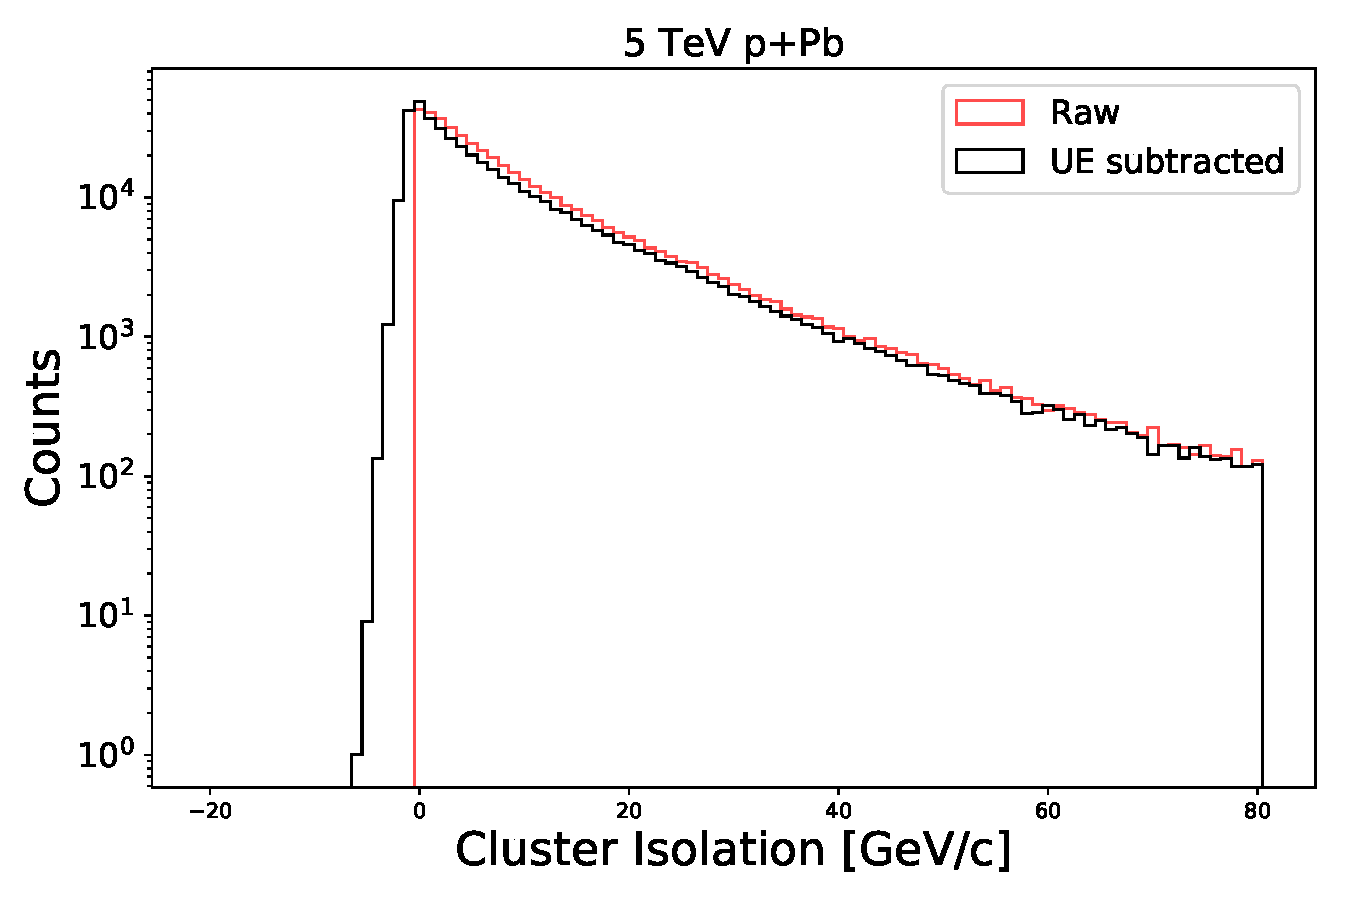
\includegraphics[width=0.49\textwidth]{Isolation/IsolationWithUESubtraction_Skimmed_13def_root}
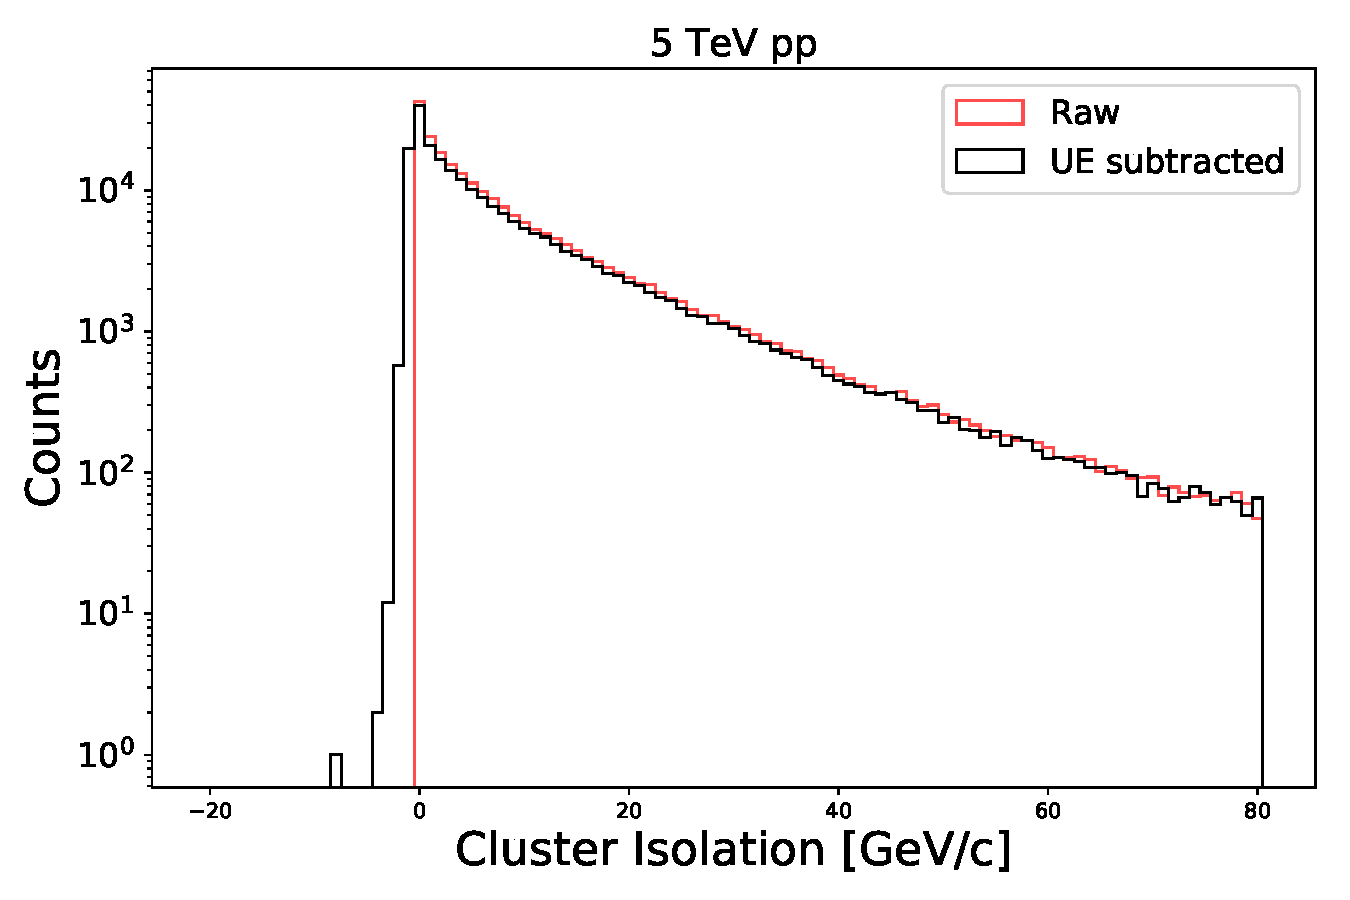
\includegraphics[width=0.49\textwidth]{Isolation/IsolationWithUESubtraction_Skimmed_17q_root}
\caption{Cluster isolation before and after underlying event subtraction in \pPb~(left panel) and pp (right panel) collisions.}
\label{fig:iso_ue}
\end{figure}

Figure~\ref{MC_Isolation} shows the distribution of cluster isolation after UE subtraction for photon-jet and dijet simulations of \pPb~data (see Table~\ref{tab:MCsamples}). As expected, the distributions are rather different: whereas the dijet simulation shows a prominent exponential tail at large $\iso$ values, the photon-jet simulation shows a Gaussian-like shape that is mostly symmetrical except for a very small fraction of events that have large $\iso$ values. In both cases, the negative tail falls rather sharply, which is expected as it arises from region-to-region fluctuations of the UE that are independent of the hard-process involved. 

\begin{figure}[h]
\center
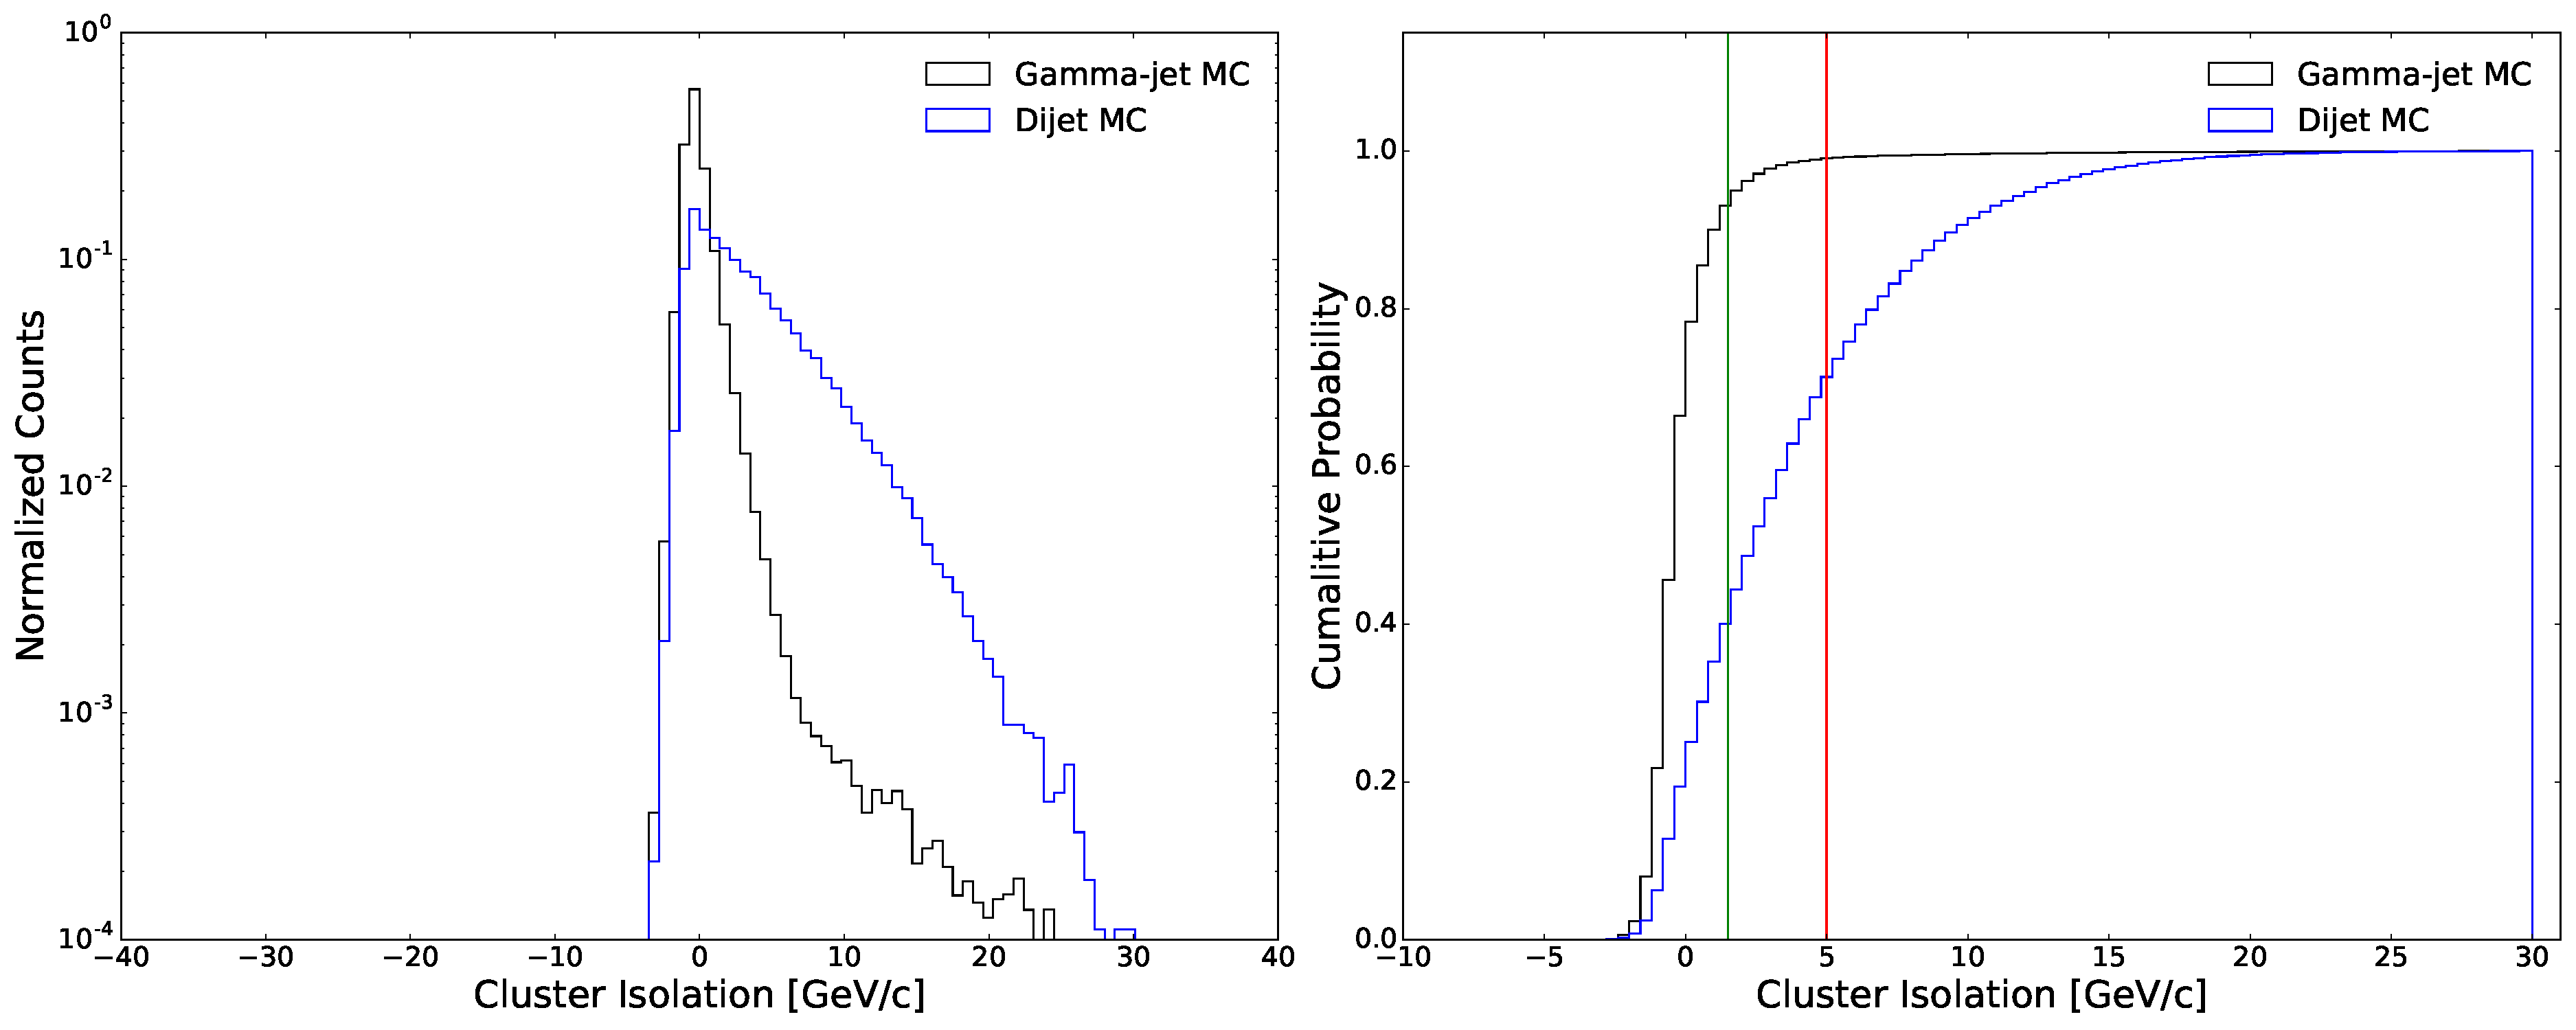
\includegraphics[width=1.0\textwidth]{Purity/Isolation_MC_pPb.pdf}
\caption{Isolation distribution of clusters that pass our selection in \pPb~photon-jet and dijet simulations, and corresponding cumulative distribution. Two vertical lines at $\iso=$ 1.5 \GeVc~(green) and $\iso=$ 5.0 \GeVc~are shown in the right panel for reference.}
\label{MC_Isolation}
\end{figure}

For the purposes of template fitting, we also need to define a sideband that is dominated by background. For this we note that only about 1$\%$ of prompt photons of the photon-jet simulation have {$\iso>$ 5 \GeVc}. Given that the cross-section for prompt photons is about two orders of magnitude smaller than the background, this region is overwhelmingly dominated by background.   
The cumulative distributions (Figure~\ref{MC_Isolation}, right panel) show that a {$\iso<$ 1.5 \GeVc} selection keeps about 90$\%$ of the signal and rejects about 60$\%$ of the background. We use this relatively loose photon isolation criteria to reduce the dependence of the results on the details of the simulation of the detector noise, tracking resolution, and the underlying event. 

This isolation cut of {$\iso<$ 1.5 \GeVc} is used in conjunction with the shower-shape cut to complete our isolated-photon selection or ``$\gammaiso$ selection''. We call ``$\gammaiso$-candidates'' the clusters that pass our isolated photon selection because it still leaves a significant fraction of background (about 40$\%$ of the cross section, as just shown). 

The main background present in our $\gammaiso$ selection is from multi-jet events where one jet typically contains a $\pi^{0}$ or $\eta$, which carries most of the jet energy, and is misidentified  as a photon because it decays into a photon pair that is collinear with respect to the EMCal cell granularity. Other sources of background arise from charged-to-neutral fluctuations of jet fragmentation that leads to low observable $\iso$ (that considers only charged-particles). 

This creates the need to measure the purity of our $\gammaiso$-candidate selection, which is described in Section~\ref{sec:purity}. 

%\subsection{Isolation efficiency}
%The isolation efficiency is ratio of the numbers of photons which pass our isolation %criteria and the rest of the cluster selection to the total number of clusters that pass the cluster selection:

%\begin{equation}
%\epsilon(\pt^{\mathrm{reco}}) = \frac{N^{\mathrm{cluster cuts + ISO cut}}(\pt^{\mathrm{reco}})}{N^{\mathrm{cluster cuts}}(\pt^{\mathrm{reco}})}.
%\end{equation}

%The cluster selection was discussed in Section~\ref{sec:clusterselection} and summarized in Table~\ref{tab:photonCutFlow}. The resulting efficiency is shown as a function of cluster \pt~in Figure~\ref{fig:isoEff}.

%The isolation efficiency is shown in Figure~\ref{fig:isoEff}. No strong dependence on $\pt$ is observed, and on average the efficiency is about 93$\%$ and 91$\%$ for pp and \pPb~ photon+jet simulated data respectively.

%We show this for illustration purposes only, because we present results normalized to the number of reconstructed photons that are, to first order, insensitive to efficiency corrections. 
%\begin{figure}[h]
%\centering
%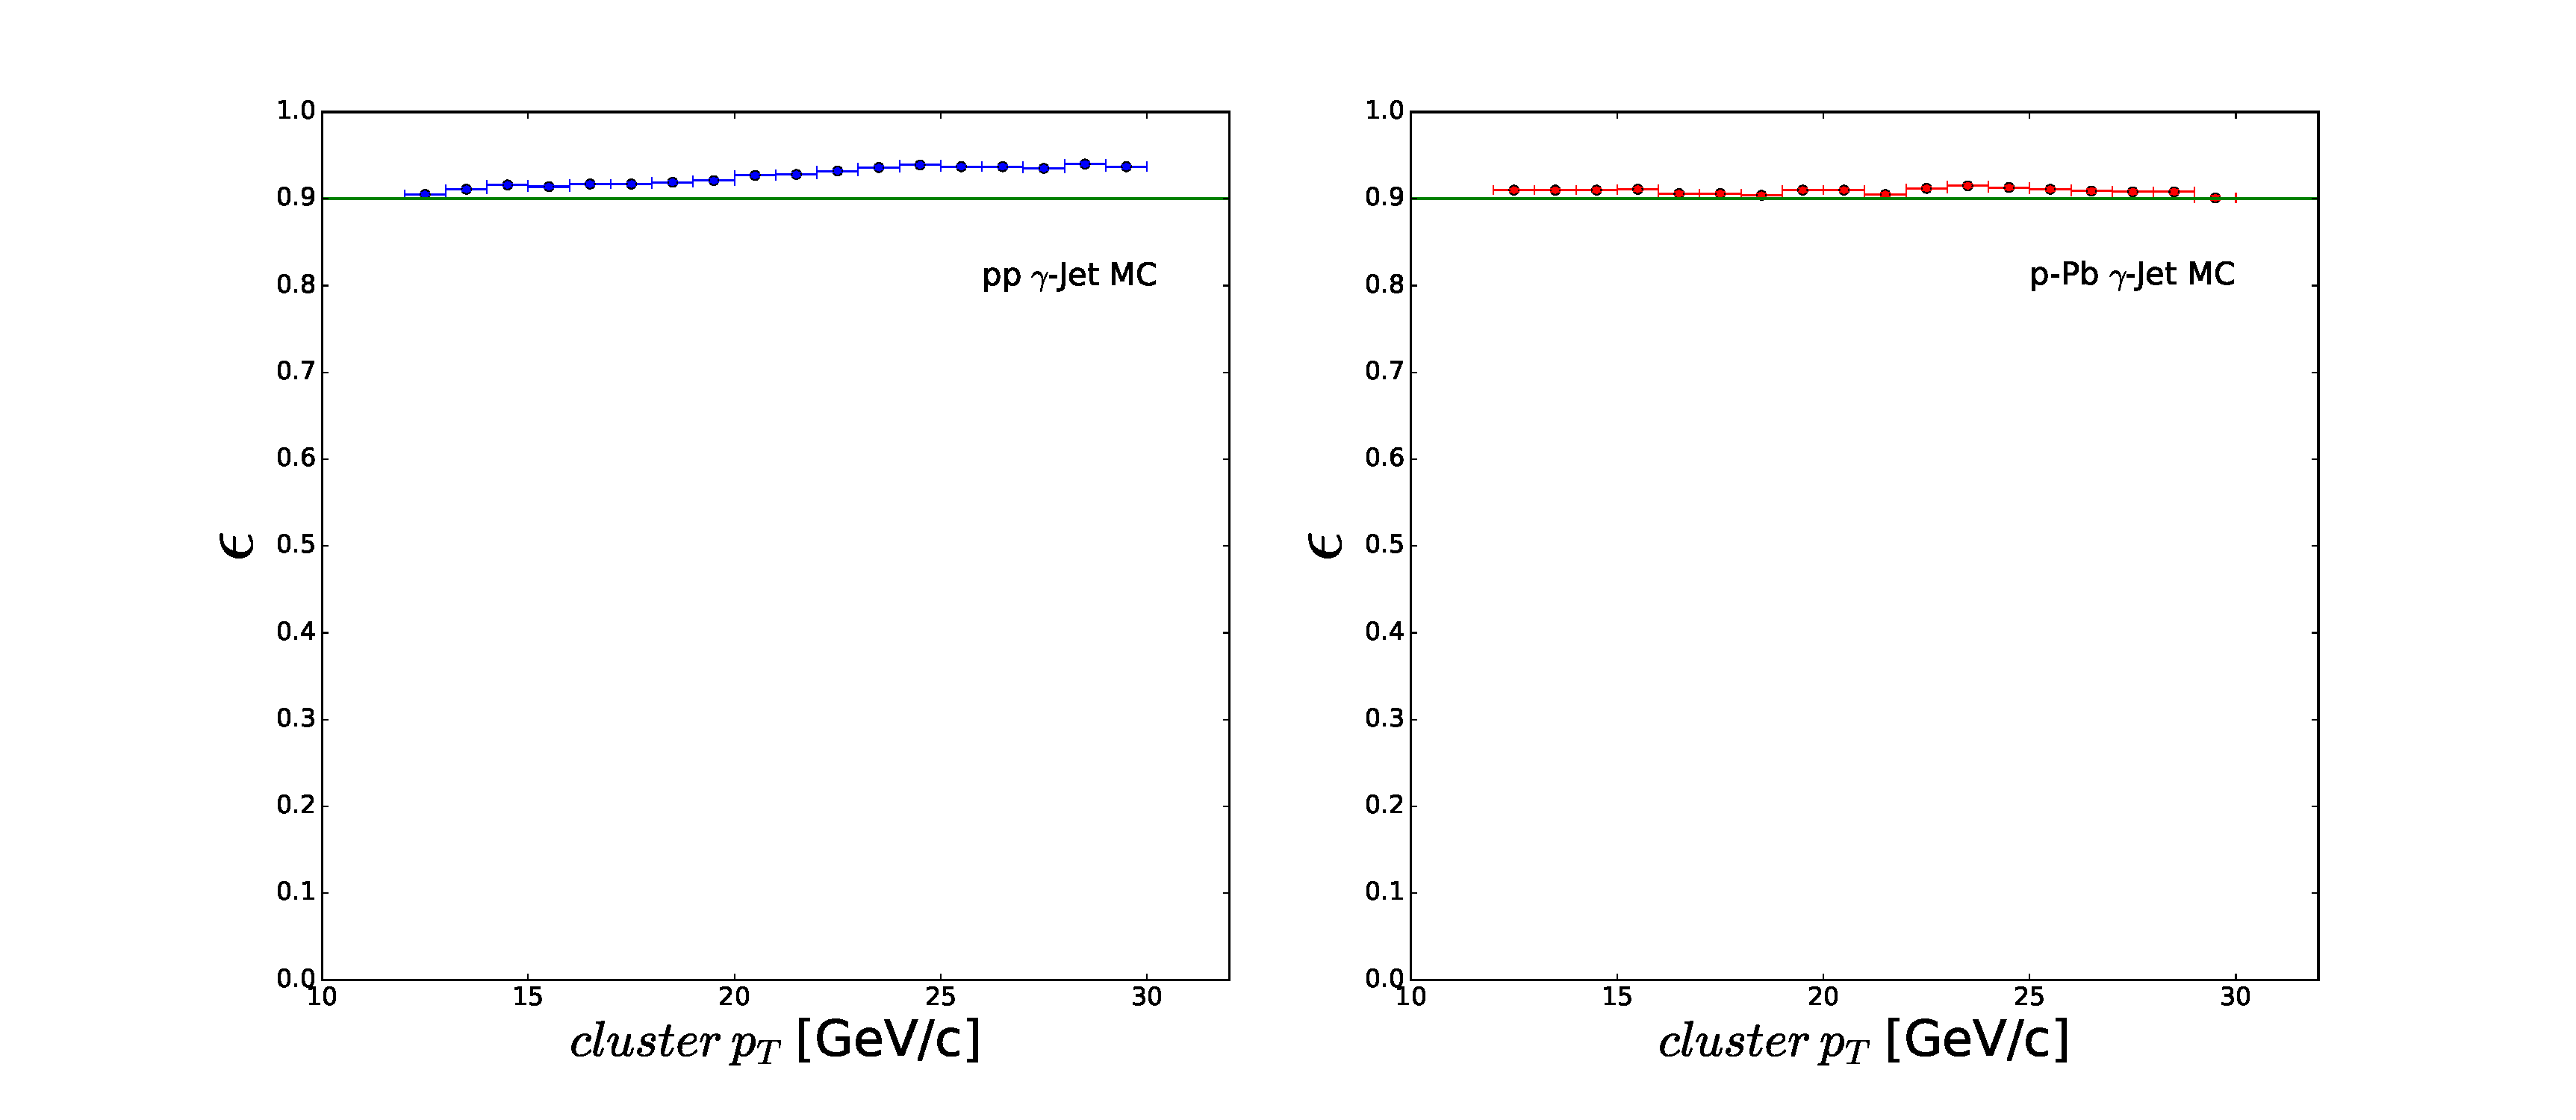
\includegraphics[width=1.0\textwidth]{EfficiencyAppendix/MC_IsoEff.pdf}
%\caption{Efficiency of isolation cut obtained from a pp and \pPb~ photon+jet simulation. A horizontal green line is placed at $\epsilon$ = 0.9 for reference. The error bars represent statistical uncertainties only.}
%\label{fig:isoEff}
%\end{figure}

%%%[still need to think about this correlation plot. Truth iso also contains UE because Pythia simulates UE. ]
%\begin{figure}[h]
%\center
%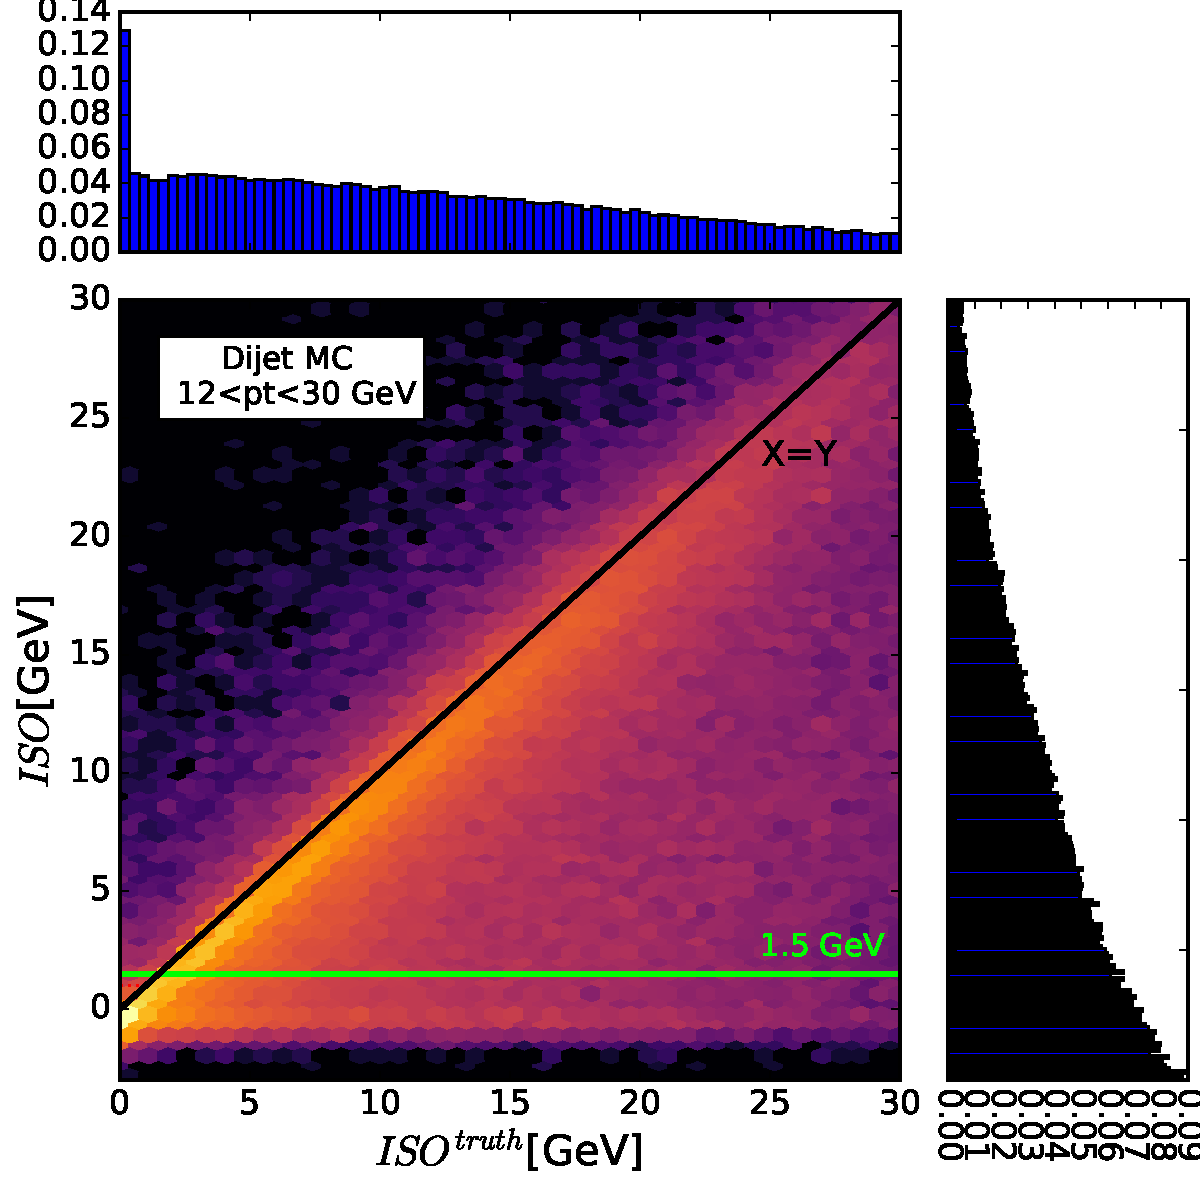
\includegraphics[height = 90mm]{Purity/pp_diject_MC.pdf}
%\caption{Correlation graph between ISO and $ISO^{truth}$ using pp Dijet MC data. The horizontal line at 1.5GeV %(green) represents the selection cut and the black is an X=Y line for reference. The correlation coefficient between ISO and $ISO^{truth}$ is found to be 70$\%$.}
%\label{pp Dijet Correlation}
%\end{figure}

\FloatBarrier
\section{Purity Measurement}
\label{sec:purity}
While the isolation requirements described in Section~\ref{sec:isolation} remove the bulk of the neutral-meson background, a substantial contribution remains; in particular, multi-jet events that produce a $\pi^{0}$ or $\eta$ that carries most of the jet energy can pass the selection. Given that the cross-section to produce a $\pi^{0}$ is much larger than the cross-section for prompt photons~\cite{Arleo:2004gn}, the background is still large for the $\pt$ range that we are interested in. In this section, we show measurements of the purity of our $\gammaiso$-candidate sample done with a template-fit method.

\subsection{Template fit method}
The purity of the isolated photon sample is determined with a two-component template fit, as was done for example by the CMS collaboration in Ref.~\cite{Sirunyan:2017qhf}. The distribution of the shower shape variable for the isolated cluster sample is fit to a linear combination of the signal distribution and the background distribution. The shape of the signal distribution is determined by a photon-jet simulation (see Table~\ref{tab:MCsamples}) and the shape of the background distribution is determined from data using an anti-isolated sideband~\footnote{The inversion of an isolation cut to estimate QCD background is a standard technique in several measurements and searches at the LHC and previous hadron colliders.} with an additional correction computed from a dijet simulation. This is described in more detail in the following sections.  

\subsubsection{Signal template and background templates }
We estimate the shape of the background distribution of the shower-shape for isolated clusters with a sideband technique. That is, we estimate the shower shape distribution of clusters from isolated decay photons with clusters that are anti-isolated but pass all other selection criteria. This method assumes that the correlation between the isolation variable and shower shape variable can be corrected for; the procedure for doing so is described below. The signal and sideband regions defined using the isolation variable are illustrated in Figure~\ref{SidebandDefinition}. 

\begin{figure}[h]
\center
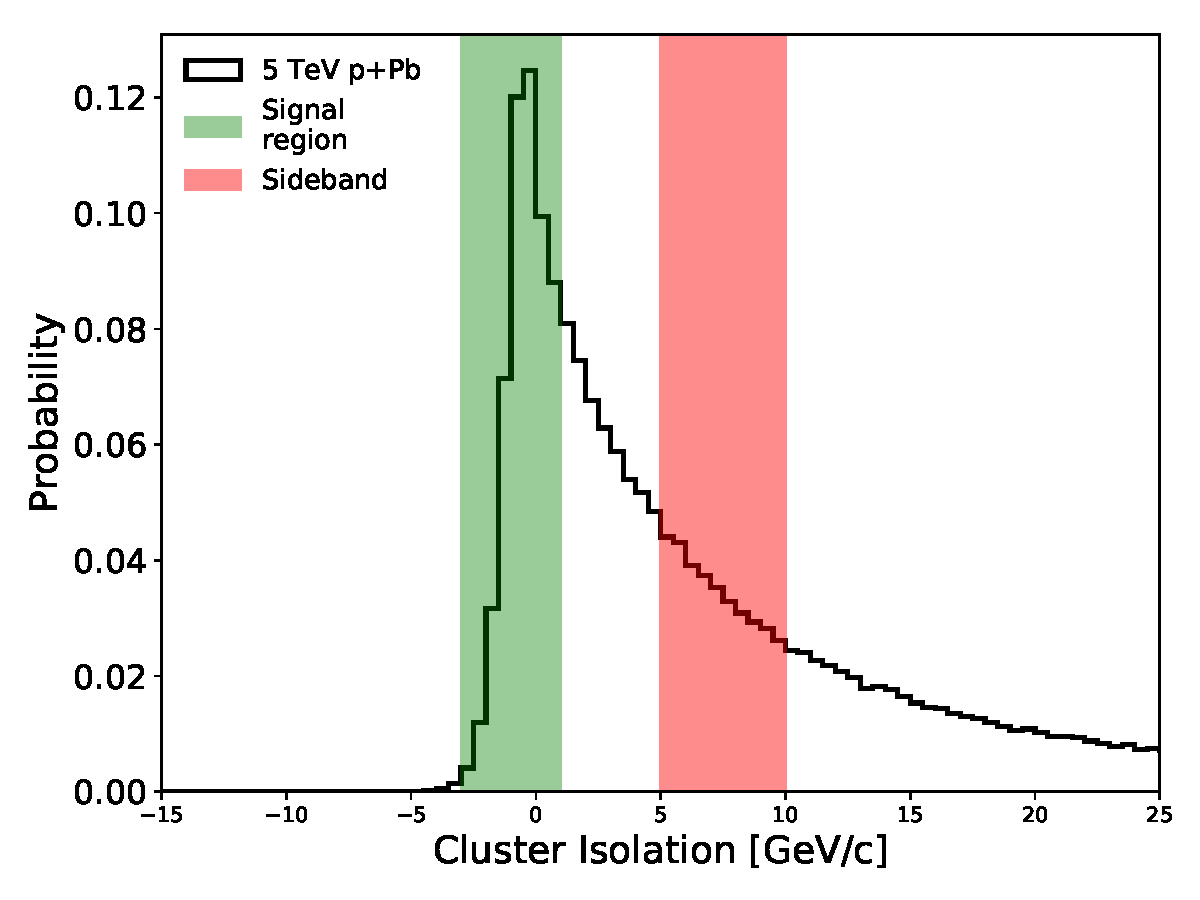
\includegraphics[width=0.49\textwidth]{Purity/IsolationSideband_limited_Skimmed_13def_root}
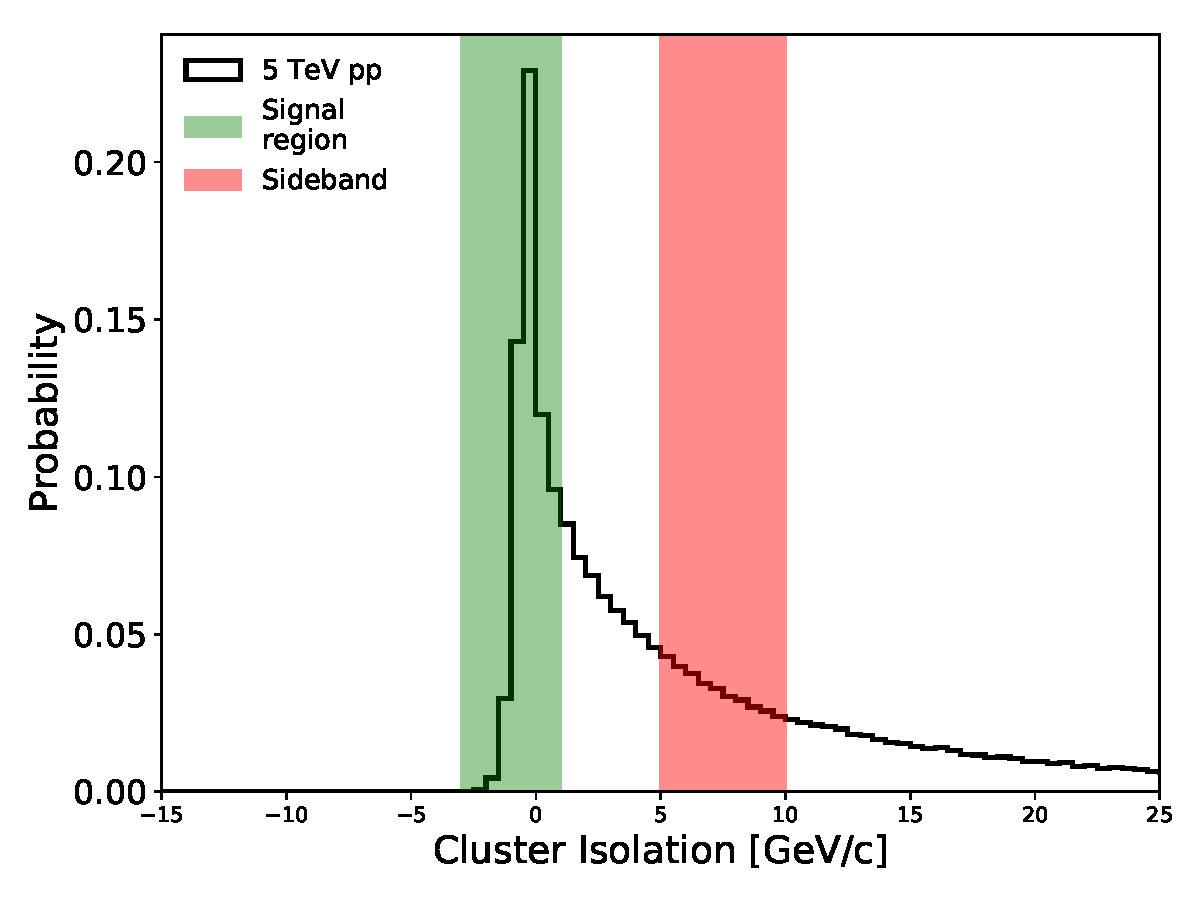
\includegraphics[width=0.49\textwidth]{Purity/IsolationSideband_limited_Skimmed_17q_root}
\caption{Isolation variable distribution of clusters with $\pt$ between 12 and 16 \GeVc~in \pPb~data (left panel) and pp data (right panel). The green shaded are represents the signal region ($\iso<$ 1.5 \GeVc); the red represent the sideband ($5<\iso<10$ \GeVc) used to estimate the background template.}
\label{SidebandDefinition}
\end{figure}

For simplicity, the same definitions are used for pp and \pPb~data. The lower bound of the sideband region is defined as {$\iso=5$ \GeVc}; according to photon-jet simulations, less than 1$\%$ of prompt photons are beyond this range. The upper bound is chosen such that the sideband is as narrow as possible, to minimize a possible bias to the shower-shape distribution due to a positive correlation with ISO, while still containing a number of clusters comparable to the signal region. A more rigorous study on the sensitivity of our purity estimate on the choice of sideband region is shown in Section~\ref{sec:bkgtemplate}.

Figure~\ref{TemplateShapes} summarizes the signal and background templates used in the template fit. The distributions are rather different, which is key for the stability of the template fit. The background shape in the $\lambdasquare$ variable shows a peak in the single-shower region but a ``bump'' that reflects a $\pi^{0}$ peak. In both cases, the peaks in the single-shower region that are observed in the background templates come mostly from collinear $\pi^{0}\to\gamma\gamma$ decays.

\begin{figure}
\center
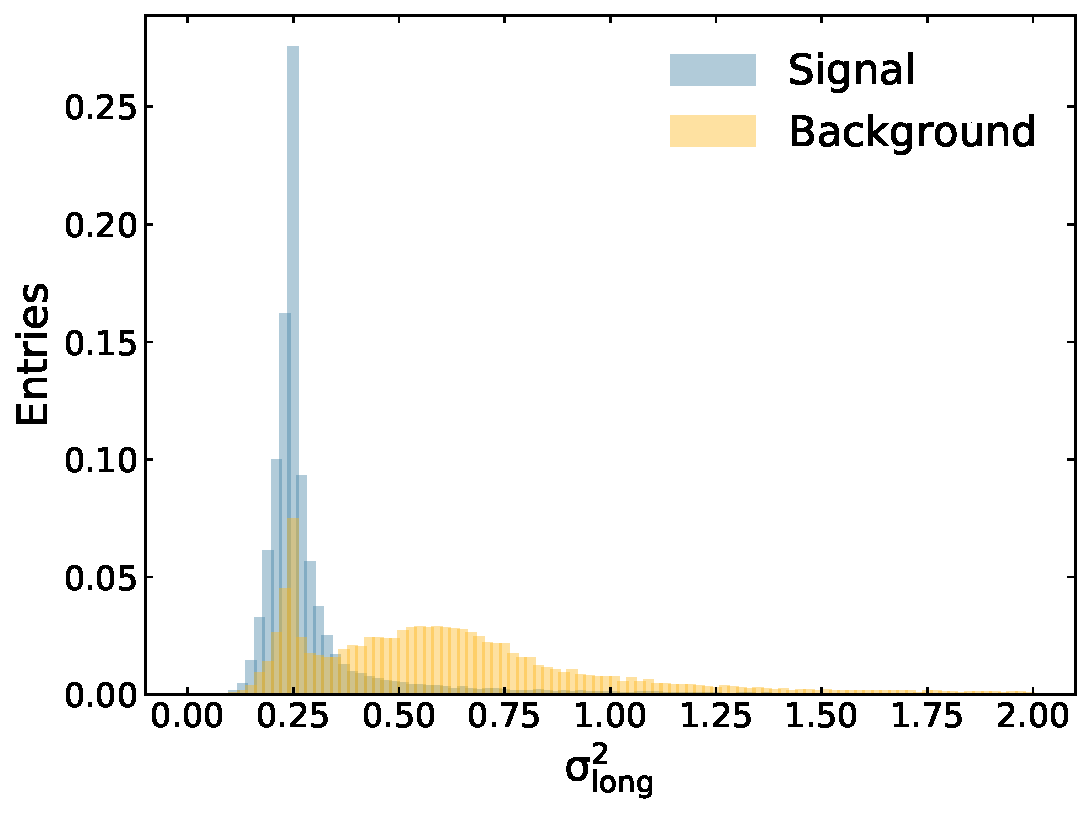
\includegraphics[width=0.49\textwidth]{Purity/norm-templates-p-Pb-cluster_Lambda-15-20.pdf}
\caption{Normalized signal (blue) and background (yellow) distributions used as input for the template fit. These distributions correspond to clusters with \pt~in the 15--20 \GeVc~range.}
\label{TemplateShapes}
\end{figure}

The background template is corrected for the correlation between the shower shape distribution and the isolation energy. A dijet simulation is used to construct the ratio of the shower shape distribution for isolated clusters to the shower shape distribution for anti-isolated clusters. This ratio, as a function of shower shape variable, is then applied as a weight to the anti-isolated clusters in the data, giving a corrected background template that is then used in the template fit (see Equation~\ref{eq:bkgtemplatecorrection}). From this equation, it is clear that, if the MC exactly replicates the data, the Weights function exactly corrects the anti-isolated decay photon \lambdasquare distribution back to the isolated decay photon \lambdasquare~distribution, which is the true background. 

\begin{align}
    \text{Weights}(\lambdasquare)&=\frac{\text{Iso}_{\text{MC}}(\lambdasquare)}{\text{Anti-iso}_{\text{MC}}(\lambdasquare)} \nonumber \\
    \text{Bkg}^{\text{corrected}}(\lambdasquare)&=\text{Non-iso}_{\text{data}}(\lambdasquare)\times\text{Weights}(\lambdasquare)
    \label{eq:bkgtemplatecorrection}
\end{align}

The purity as computed with the corrected background template is 8--13\% lower in absolute value as compared to the purity as computed with the uncorrected background template; an example of a fit with and without the correction is shown in Figure~\ref{fig:purcorrectionexample}. The correction greatly improves the goodness-of-fit. The $\text{Weights}(\lambdasquare)$ function for different \pt~ranges is shown in Appendix~\ref{sec:MCbasedcorrection} and the evaluation of the systematic uncertainty associated with this correction is described in Section~\ref{sec:puritysystematics}. 

\FloatBarrier
\begin{figure}
    \centering
    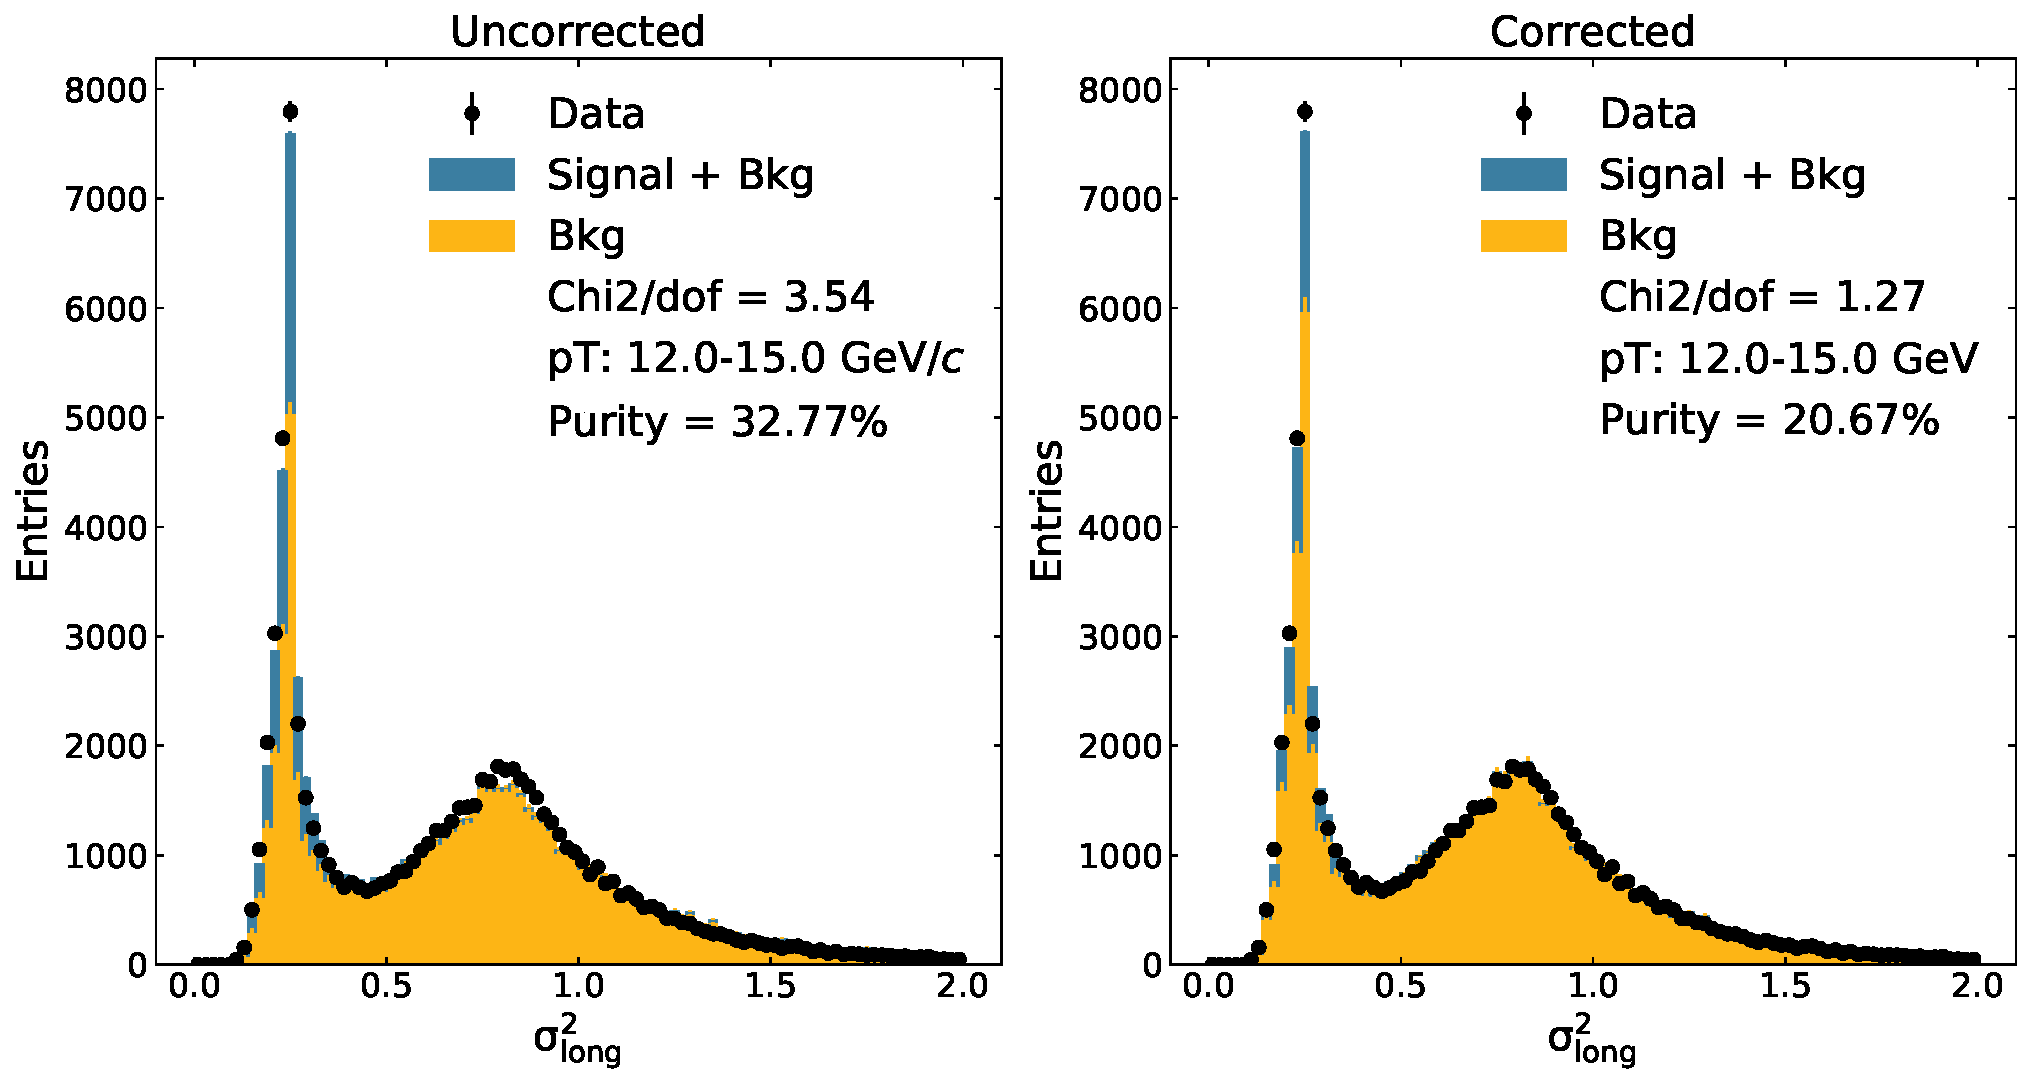
\includegraphics[width=\textwidth]{Purity/correction-example-p-Pb-cluster_Lambda-12-15.pdf}
    \caption{An example of the template fit with and without the background template correction in \pPb~for clusters with $12 < \pt < 15$ GeV/$c$. The goodness of fit is better after the correction and the purity is significantly lower.}
    \label{fig:purcorrectionexample}
\end{figure}


\subsubsection{Fit results}
\label{sec:fitresults}
The distribution of isolated clusters is fit with a linear combination of the signal and background templates. We use the \textsc{MINUIT}~\cite{James:1975dr} package for $\chi^{2}$ minimization and the \textsc{MIGRAD} package for error estimation. The only free parameter in the fit is the number of signal clusters, $N_{\mathrm{sig}}$, because the overall normalization, $N$, is fixed to the total number of isolated clusters:
\begin{equation}
N^{\mathrm{observed}} = N_{\mathrm{sig}}\times S + (N-N_{\mathrm{sig}})\times B,
\end{equation}
where $S$ and $B$ are the normalized signal template and background template. 


Figures~\ref{TemplatefitResults_Preliminary} show template fit results for \pPb~and pp data. In all cases a good fit with no systematic pattern in the residuals is achieved over most of the distribution, and the reduced $\chi^{2}$ ranges within acceptable values. The purity measurements are presented in graphical form in Figure~\ref{fig:purityresults}. 


\begin{figure}[h]
\center
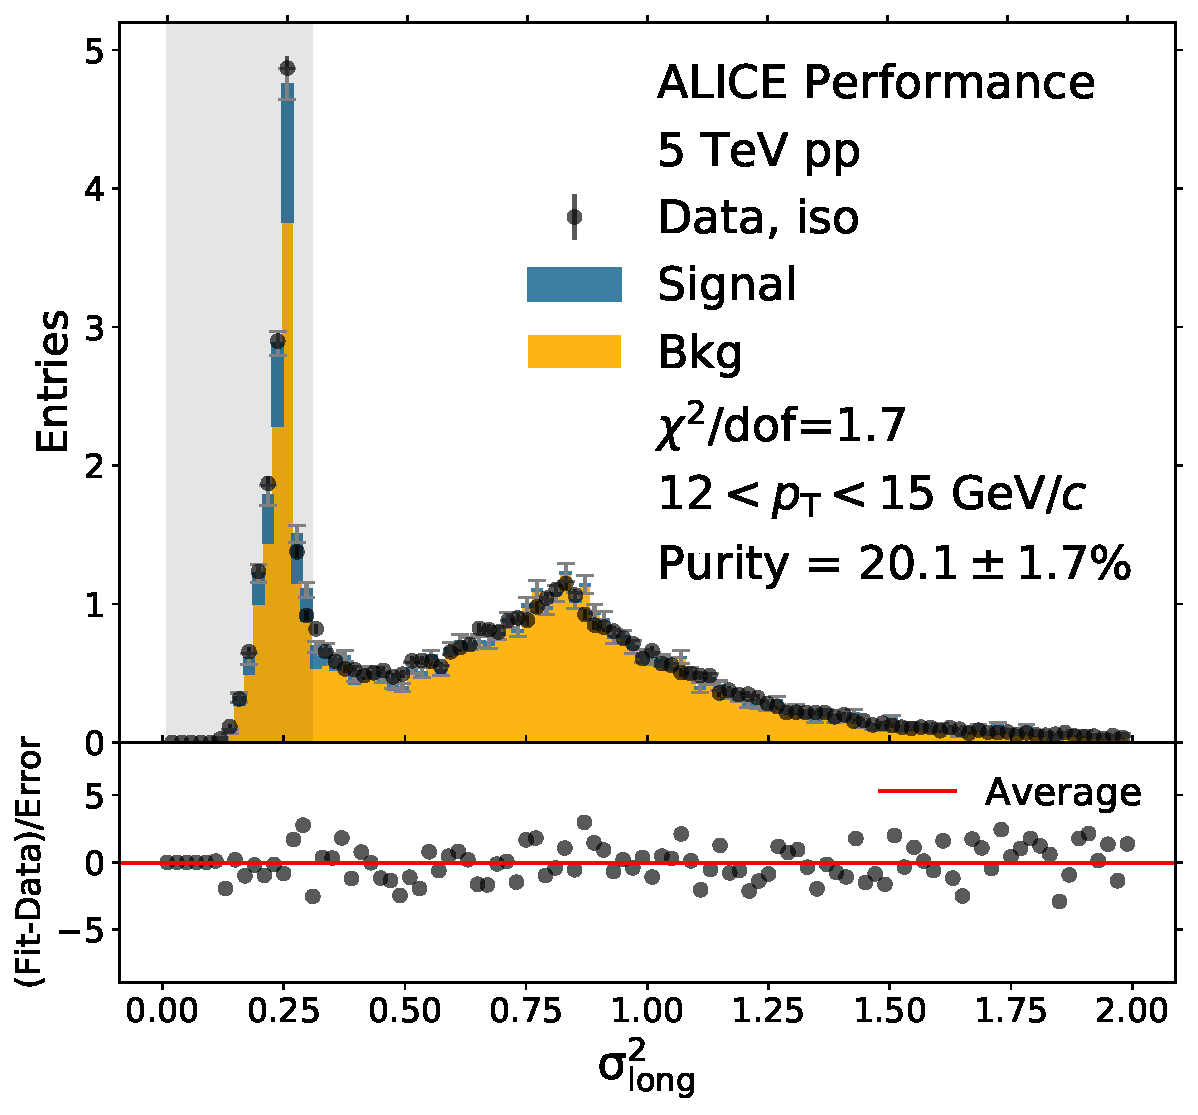
\includegraphics[width=0.38\textwidth]{Purity/tf-example-pp-cluster_Lambda-12-15.pdf}
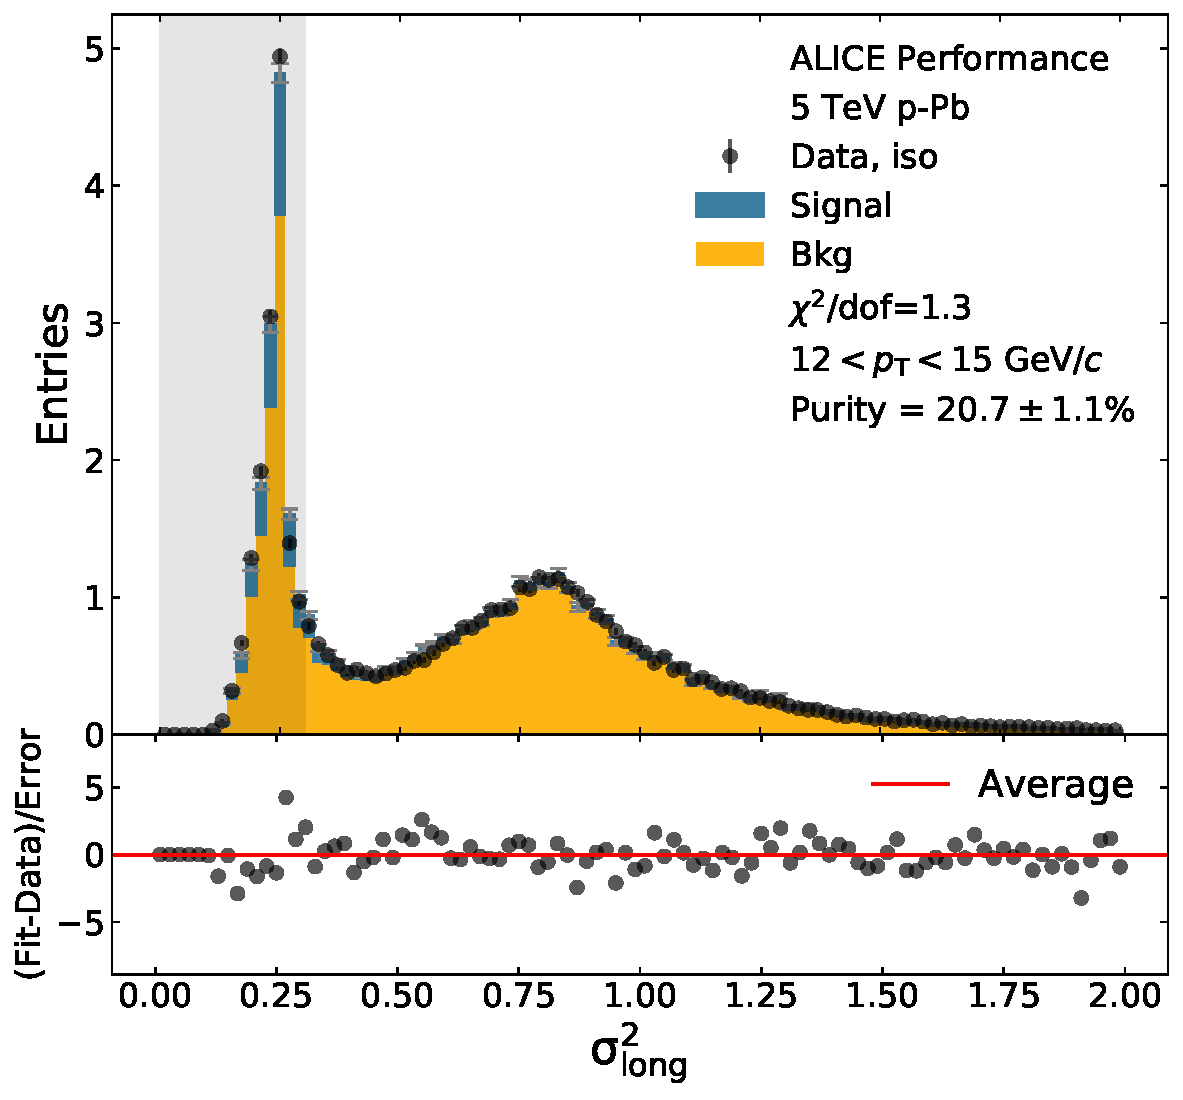
\includegraphics[width=0.38\textwidth]{Purity/tf-example-p-Pb-cluster_Lambda-12-15.pdf}
\\
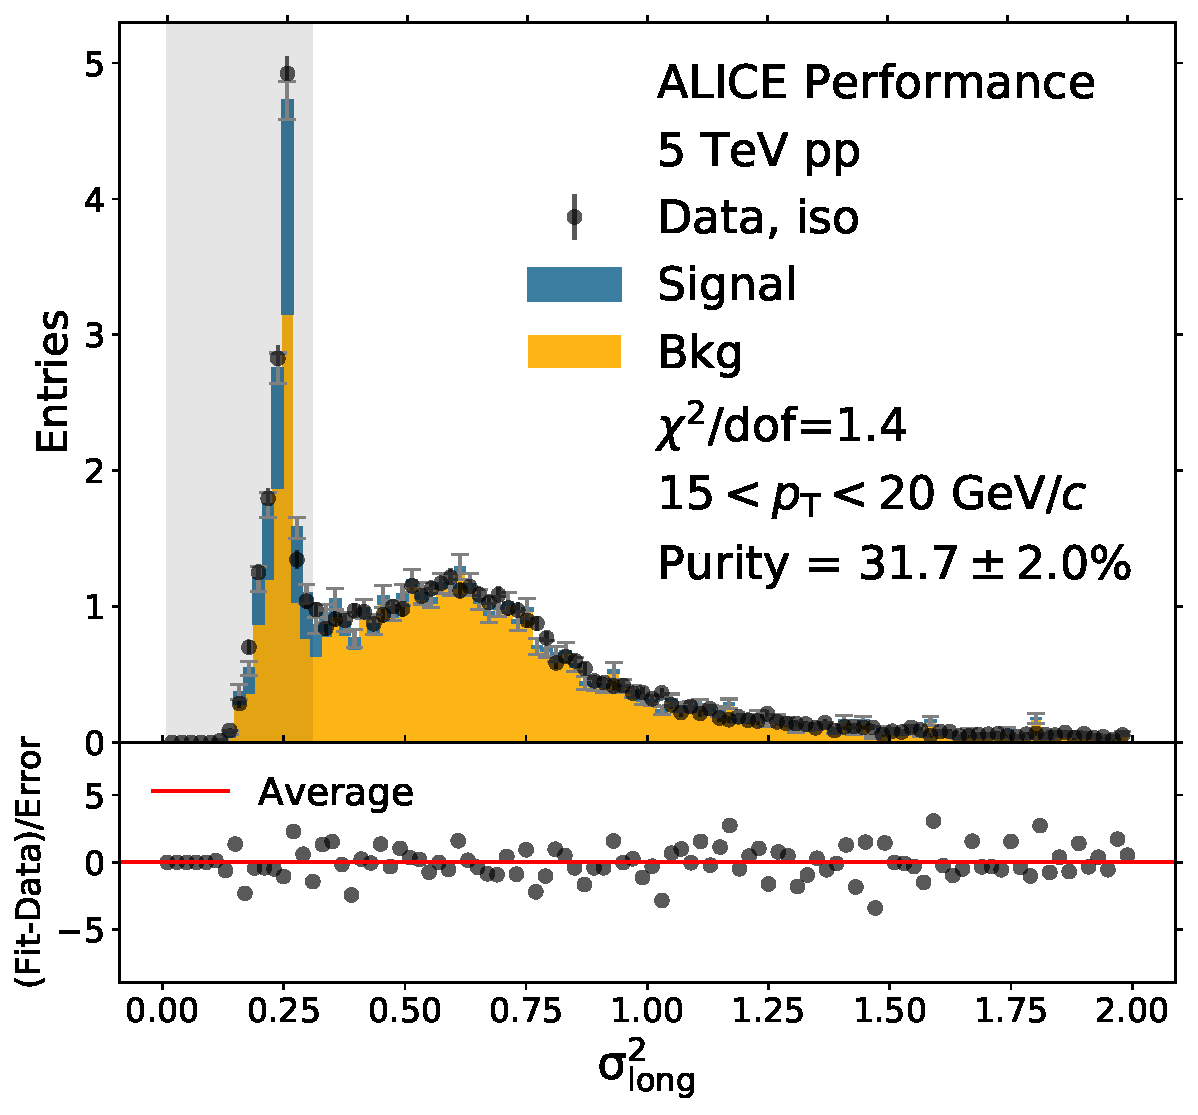
\includegraphics[width=0.38\textwidth]{Purity/tf-example-pp-cluster_Lambda-15-20.pdf}
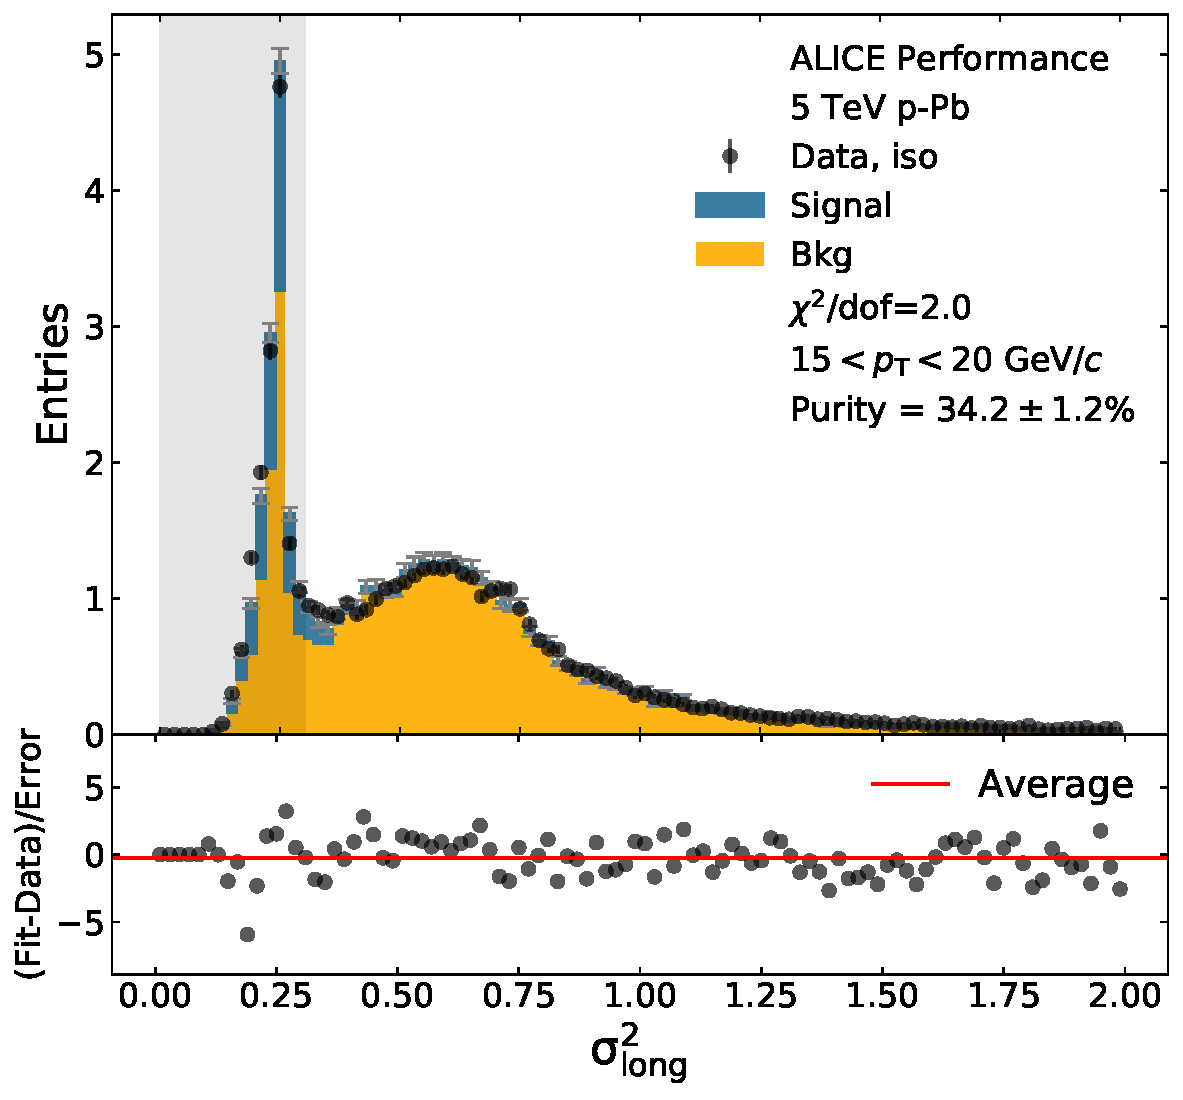
\includegraphics[width=0.38\textwidth]{Purity/tf-example-p-Pb-cluster_Lambda-15-20.pdf}
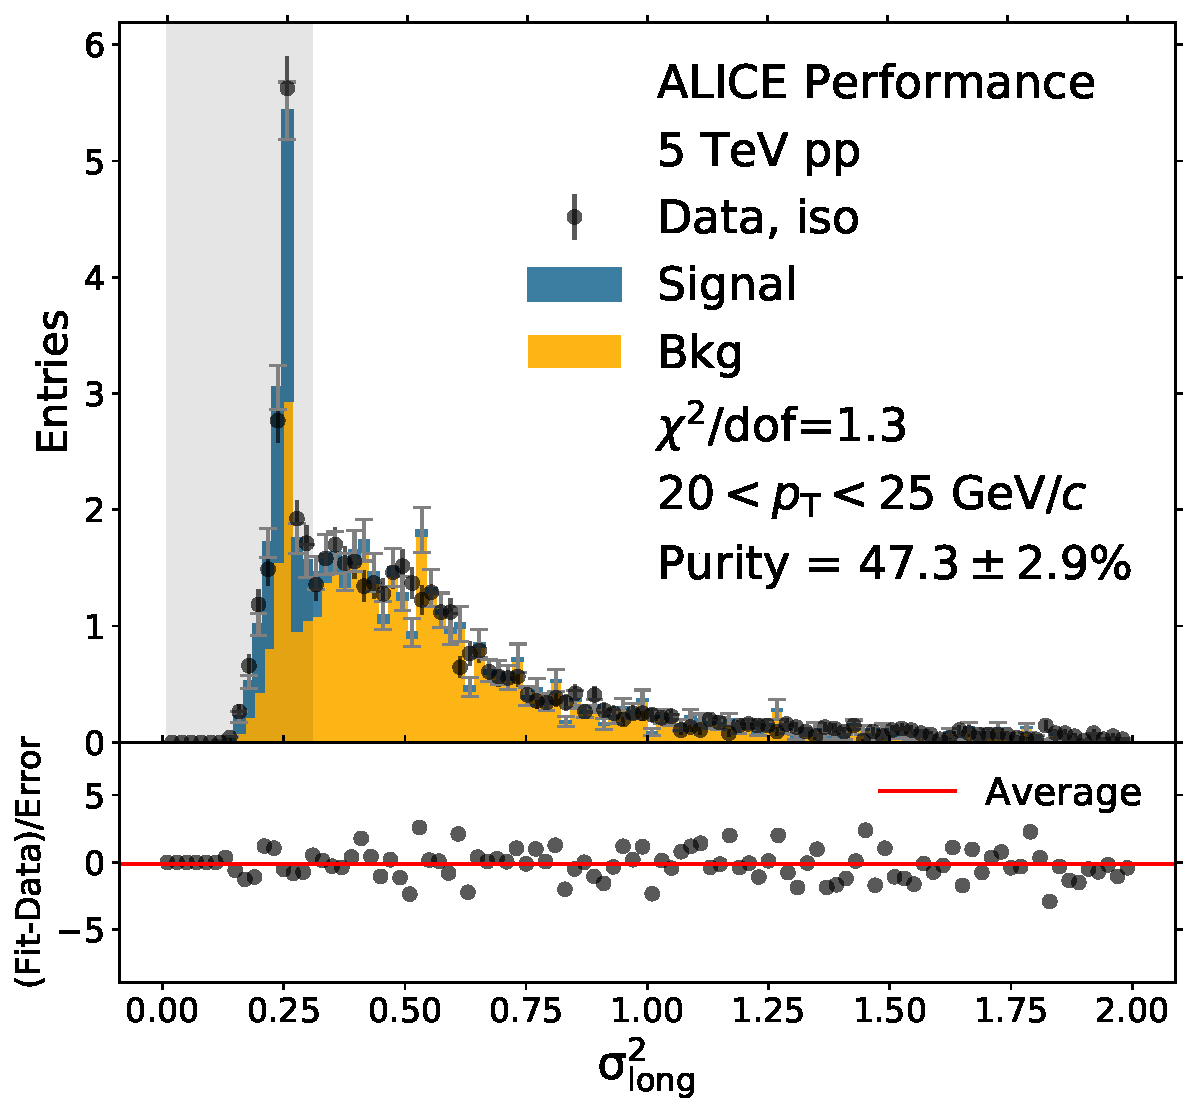
\includegraphics[width=0.38\textwidth]{Purity/tf-example-pp-cluster_Lambda-20-25.pdf}
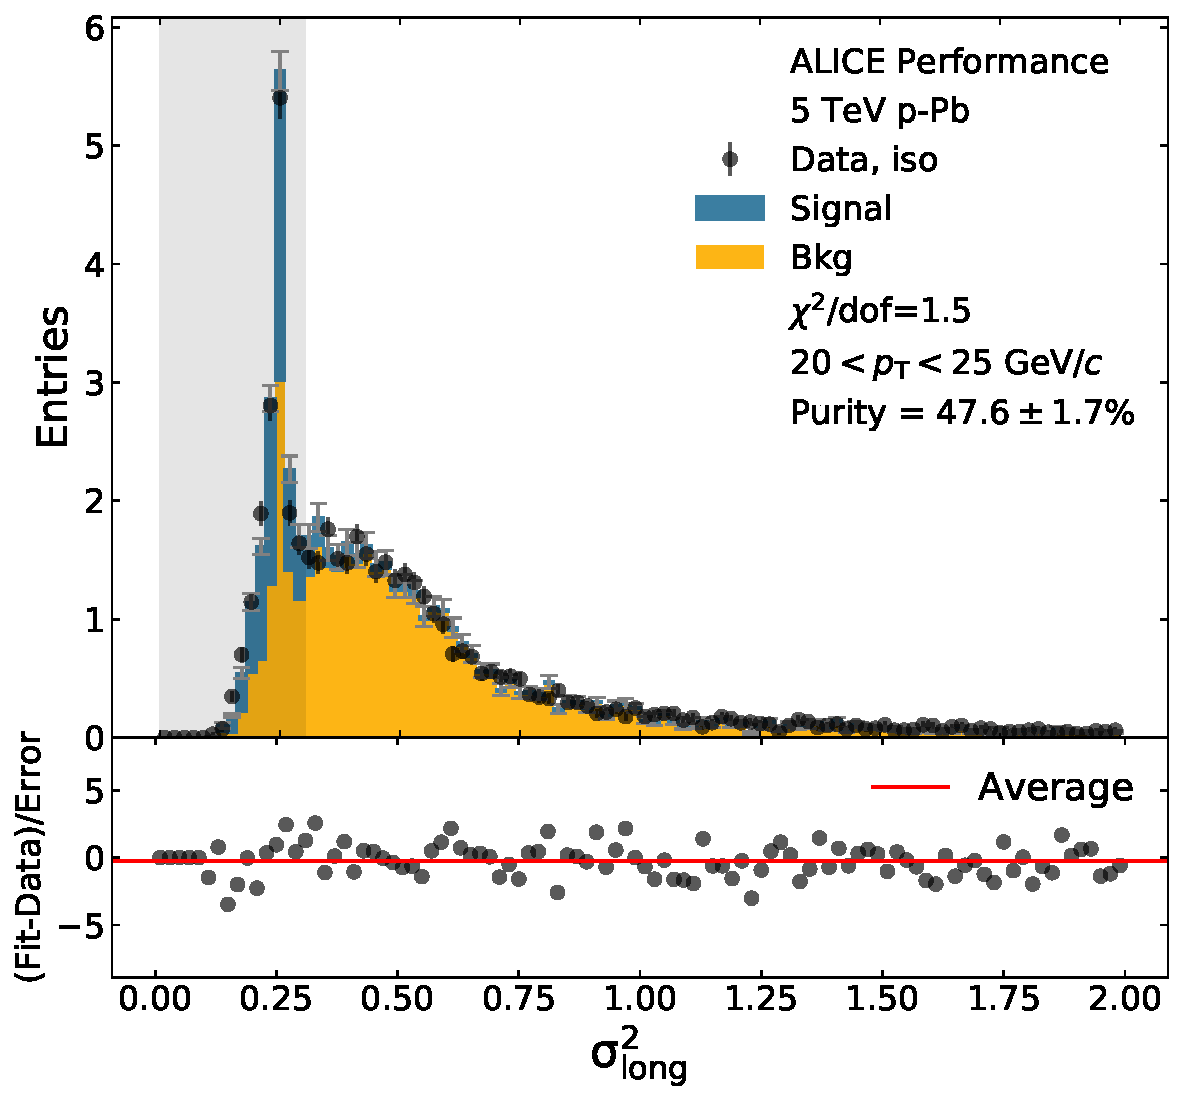
\includegraphics[width=0.38\textwidth]{Purity/tf-example-p-Pb-cluster_Lambda-20-25.pdf}
\\
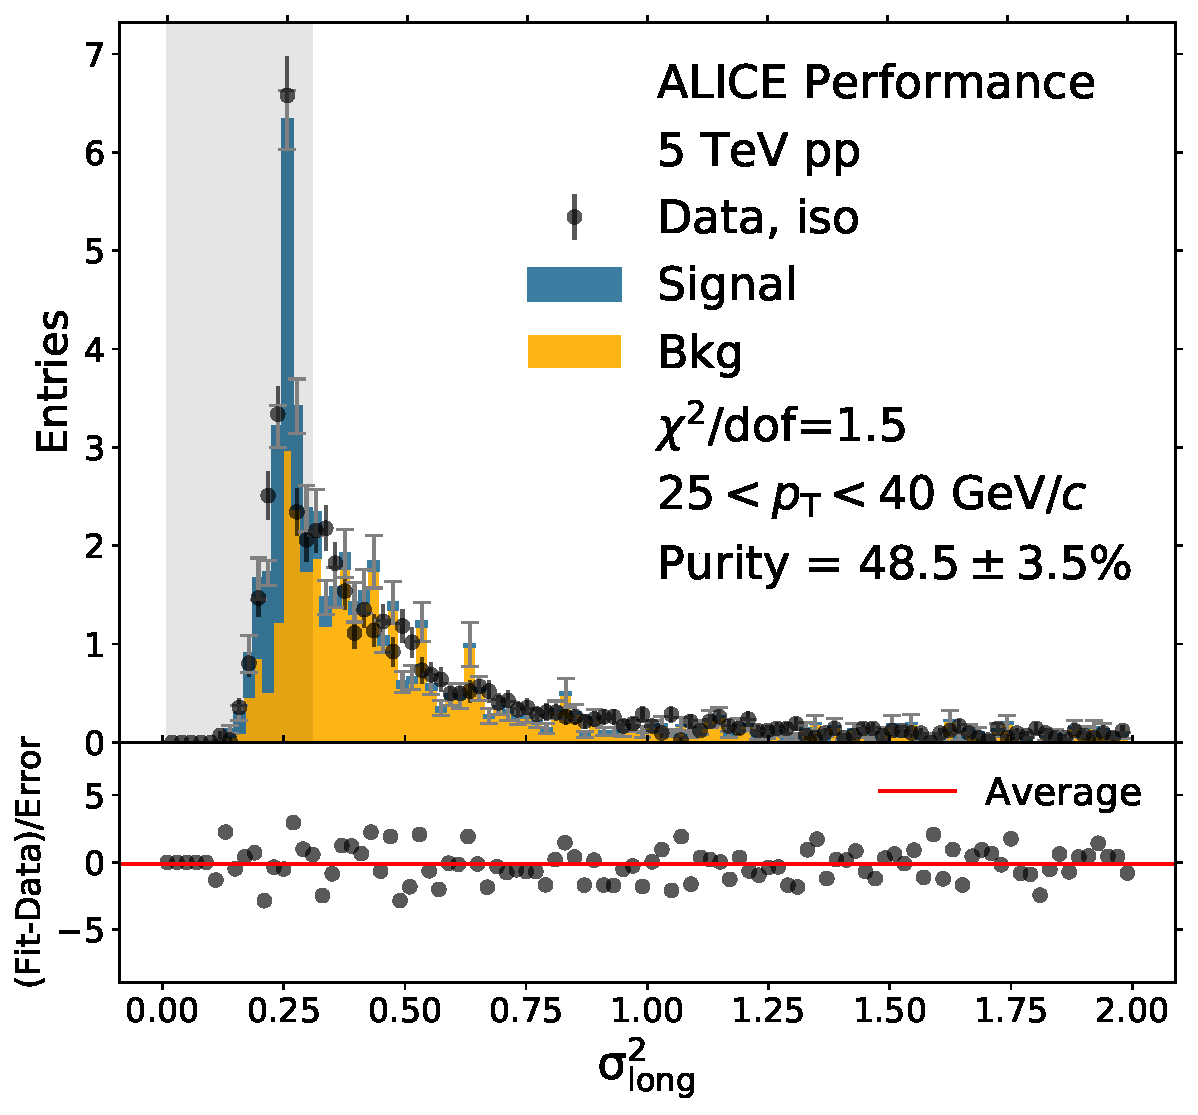
\includegraphics[width=0.38\textwidth]{Purity/tf-example-pp-cluster_Lambda-25-40.pdf}
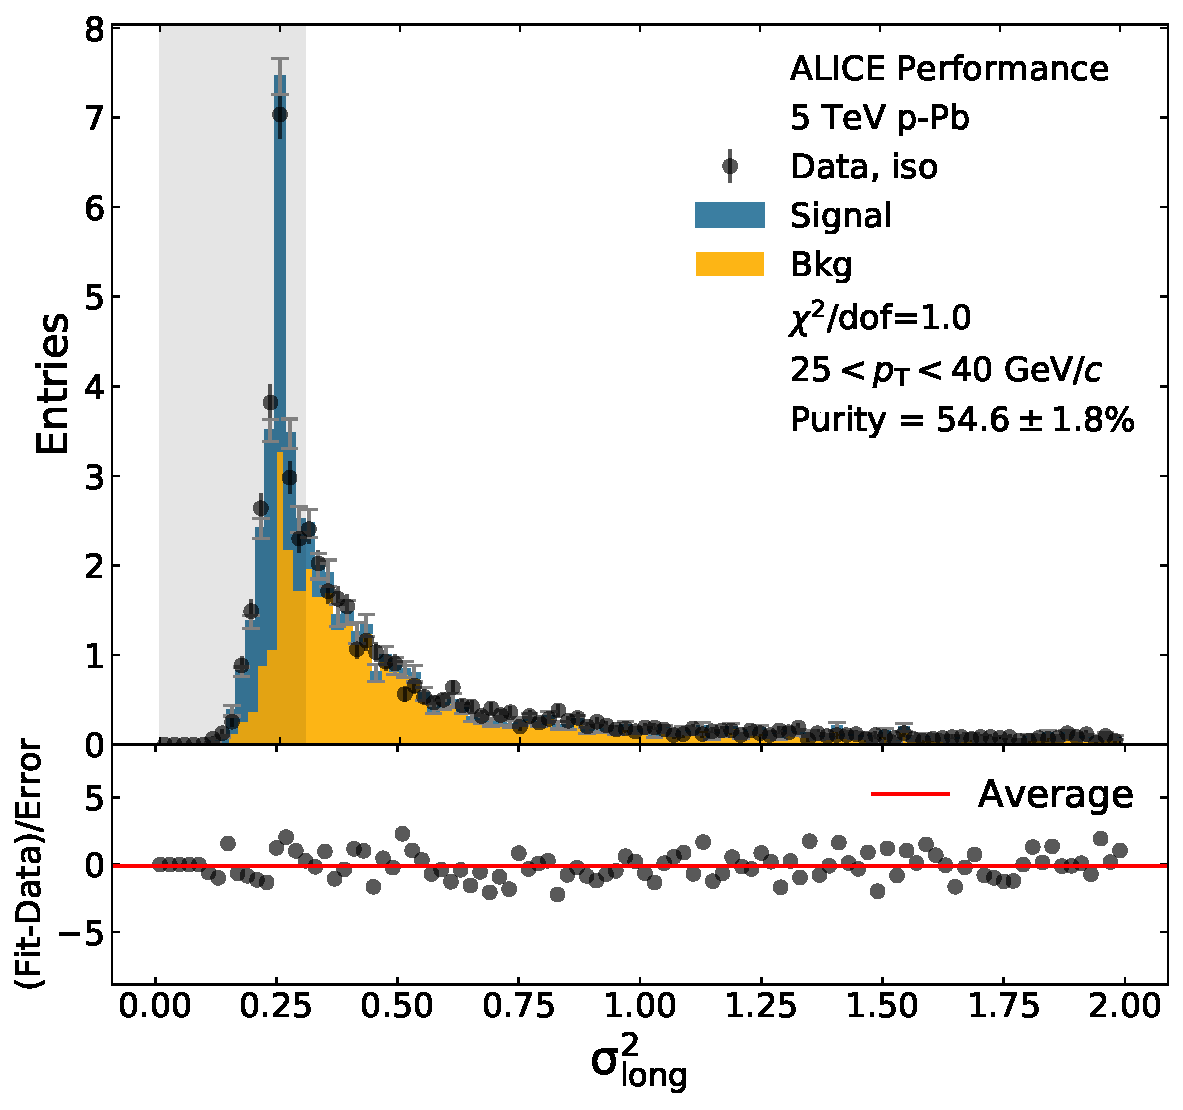
\includegraphics[width=0.38\textwidth]{Purity/tf-example-p-Pb-cluster_Lambda-25-40.pdf}
\caption{Template fit results in pp and \pPb~data. The stacked histograms (yellow for background, blue for signal) are the predicted counts given the best-fit value of the number of signal photons, $N_{\mathrm{sig}}$. The hatched gray area represents the interval considered for the purity estimate. The bottom panels show the normalized residuals of the fit, considering the statistical uncertainty on the isolated cluster data and the background template added in quadrature. }
\label{TemplatefitResults_Preliminary}
\end{figure}

%\begin{table}
%   \caption{Impact of the \gammaiso selection variations on purity measurement on pp and \pPb~data. The nominal isolation selection is changed to $\iso<$1.50 $\pm$ 0.25 \GeVc; the nominal shower-shape selection is changed to  $\lambdasquare<0.30 \pm 0.03$}
%   \label{tab:variationspurity}
    % \begin{tabular*}{1.0\columnwidth}{@{\extracolsep{\fill}}l|llllll@{}}
    % 	\hline
    % 	 & Nominal & $\iso < 1.25$ \GeVc & $\iso < 1.75$ \GeVc & $\lambdasquare < 0.27$ & $\lambdasquare < 0.33$ \\
    % 	\hline
    % 	pp data & & & & & \\
    % 	\hline
    % 	12--15 \GeVc & 16.9 & 18.2 & 15.9 & 16.5 & 16.9 \\
    % 	15--20 \GeVc & 29.5 & 31.0 & 28.0 & 29.3 & 29.1 \\
    % 	20--25 \GeVc & 46.8 & 48.4 & 45.4 & 49.1 & 44.9 \\
    % 	25--40 \GeVc & 48.0 & 49.3 & 46.7 & 55.9 & 45.1 \\
    % 	\hline
    % 	p-Pb data & & & & & \\
    % 	\hline
    % 	12--15 \GeVc & 20.7 & 21.5 & 19.7 & 20.2 & 20.5 \\
    % 	15--20 \GeVc & 34.2 & 35.5 & 33.1 & 34.3 & 33.6 \\
    % 	20--25 \GeVc & 47.6 & 49.0 & 46.5 & 51.7 & 44.9 \\
    % 	25--40 \GeVc & 54.6 & 56.8 & 52.8 & 62.1 & 51.1 \\
    % 	\hline
    % \end{tabular*}
%\end{table}









\begin{figure}[h]
\center
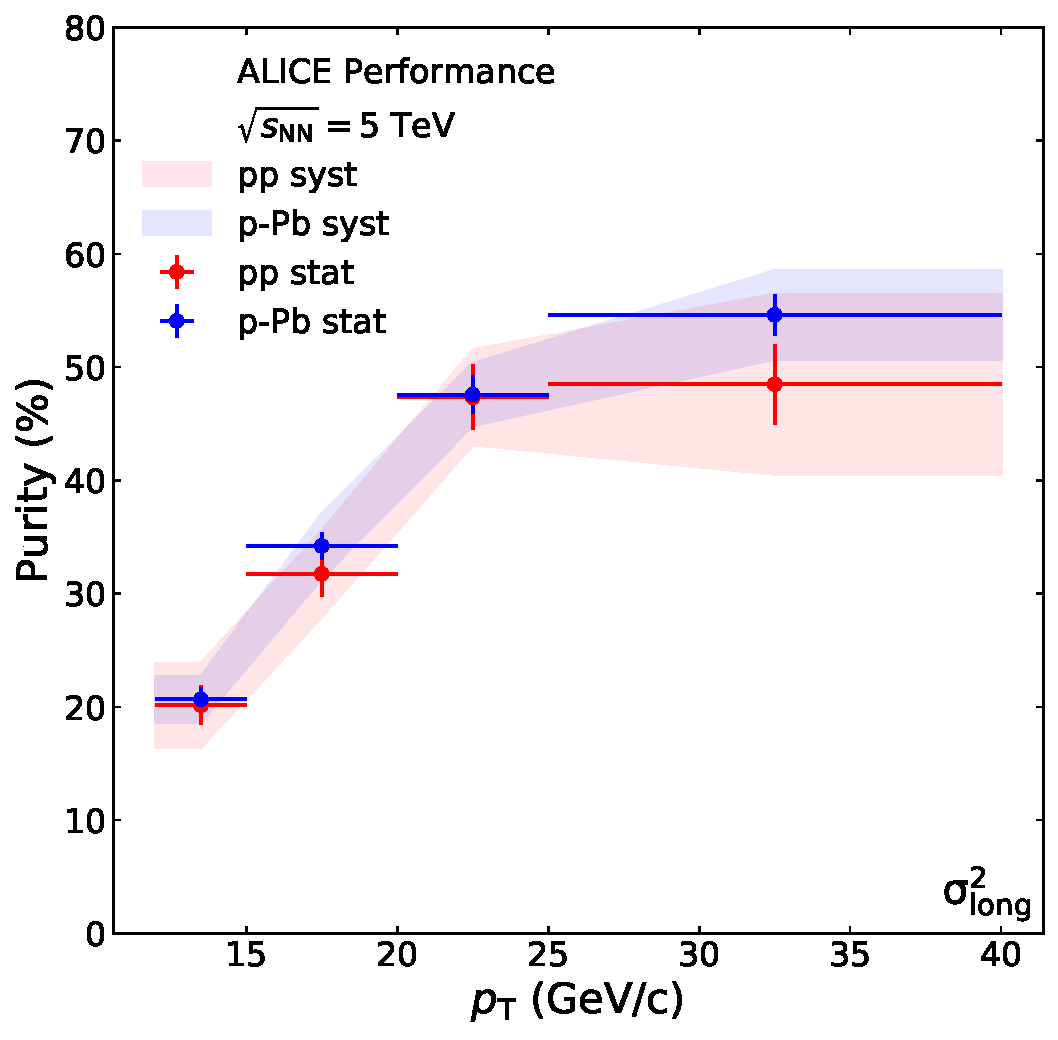
\includegraphics[width=0.495\textwidth]{Purity/purities-combined-cluster_Lambda.pdf}
\caption{Purity of isolated-photon selection as a function of cluster \pt. The error bar represents statistical uncertainty only. The error band represents the systematic uncertainty only.}
\label{fig:purityresults}
\end{figure}

\FloatBarrier
%%%%%%%%%%%%%%%%%%%%%%%%%%%%%%%
\subsection{Systematic uncertainties of the purity measurement}
\label{sec:puritysystematics}
There are two assumptions underlying the template fit procedure. The first is that the signal template from simulations is correct. The second is that the shape of the background estimated from the anti-isolated sideband, with the correction coming from simulations, reflects the shape of the background in the signal region. That is, the assumption is that the correlation between the shower shape and isolation variables can be corrected for via an appropriate simulation. The dominant sources of systematic uncertainty on this measurement are described in this section and can be summarized as follows: the signal template, the sideband region selection, and the background template correction. We also investigated the effect of varying our cluster selection but found that the variations on the purity measurements are much smaller than the other sources of systematic uncertainties investigated here, so we neglect that. This is shown in Appendix~\ref{sec:clustercutselectionvariation}. 

\subsubsection{Signal template}
We estimate the systematic uncertainty on the purity estimate due to imperfections in the signal template by using a data-driven template fit. In this, we restrict the range of the $\chi^{2}$ fit to the background-dominated region of the shower-shape distribution (0.4--1.5 for $\lambdasquare$) and we use only the background template to fit the isolated data with the normalization as the only free parameter. To factorize the effect of the MC-correction to the background template, we do not apply it for this study. Once the background normalization is fitted, we consider the signal to be the integral of the isolated data minus the integral of the background, both in the signal region of the shower-shape variable. 

Figure~\ref{BkgOnlyFit_pPb} show the results obtained with this method in pp and \pPb~data. We observe some systematic pattern in the residuals, which can be attributed to the lack of MC-correction on the background template. 

\begin{figure}[h]
\center
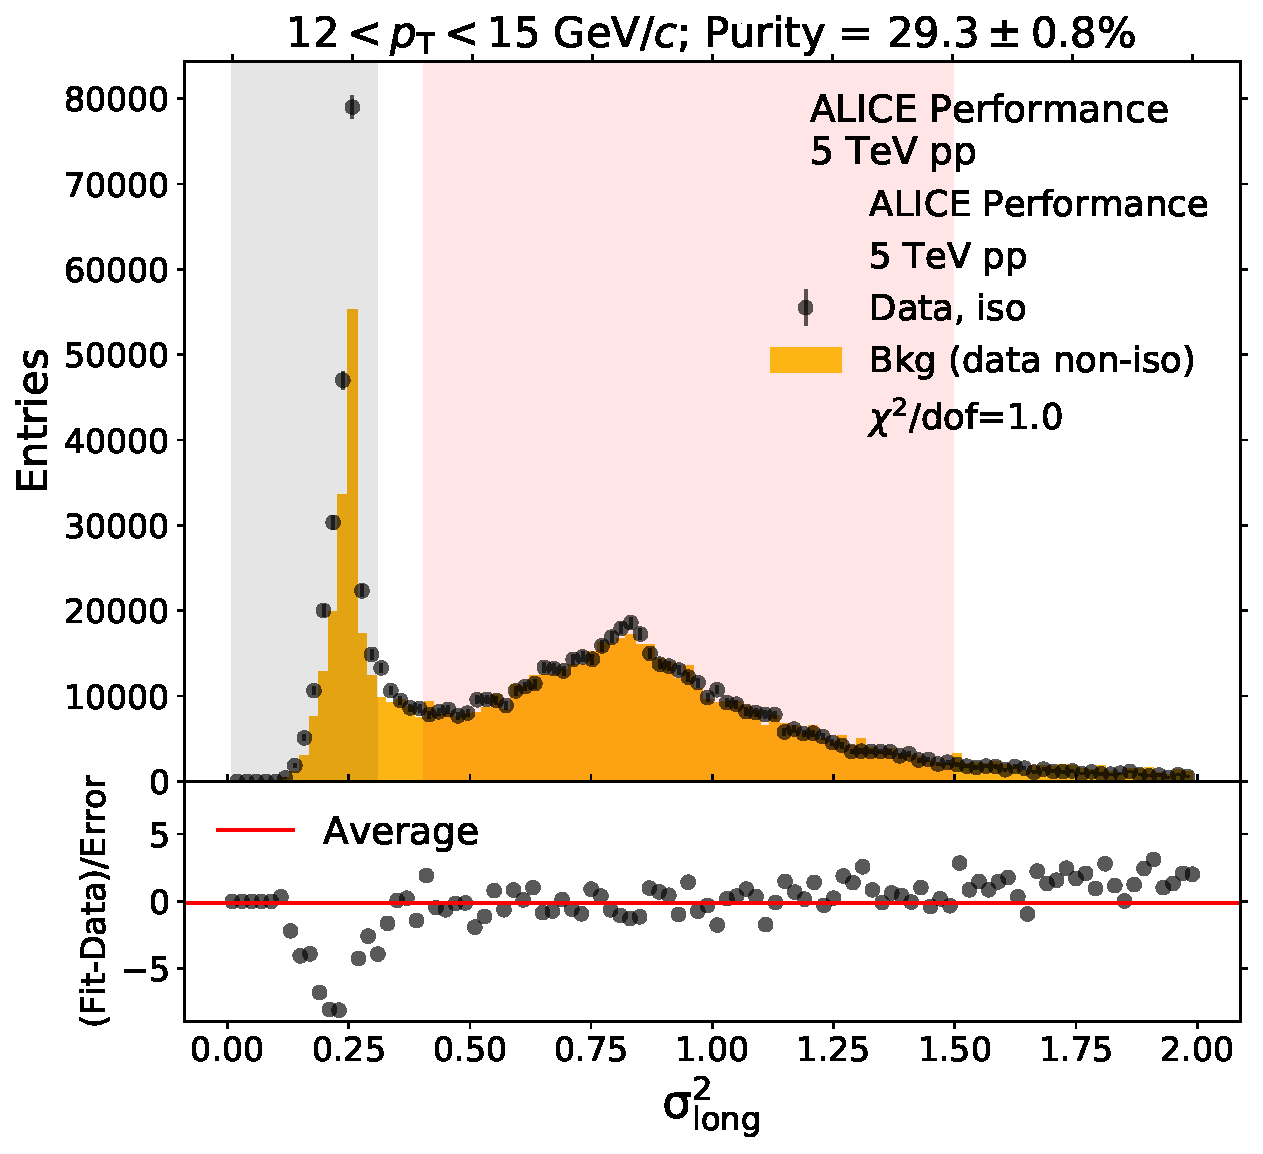
\includegraphics[width=0.38\textwidth]{Purity/bf-example-pp-cluster_Lambda-12-15.pdf}
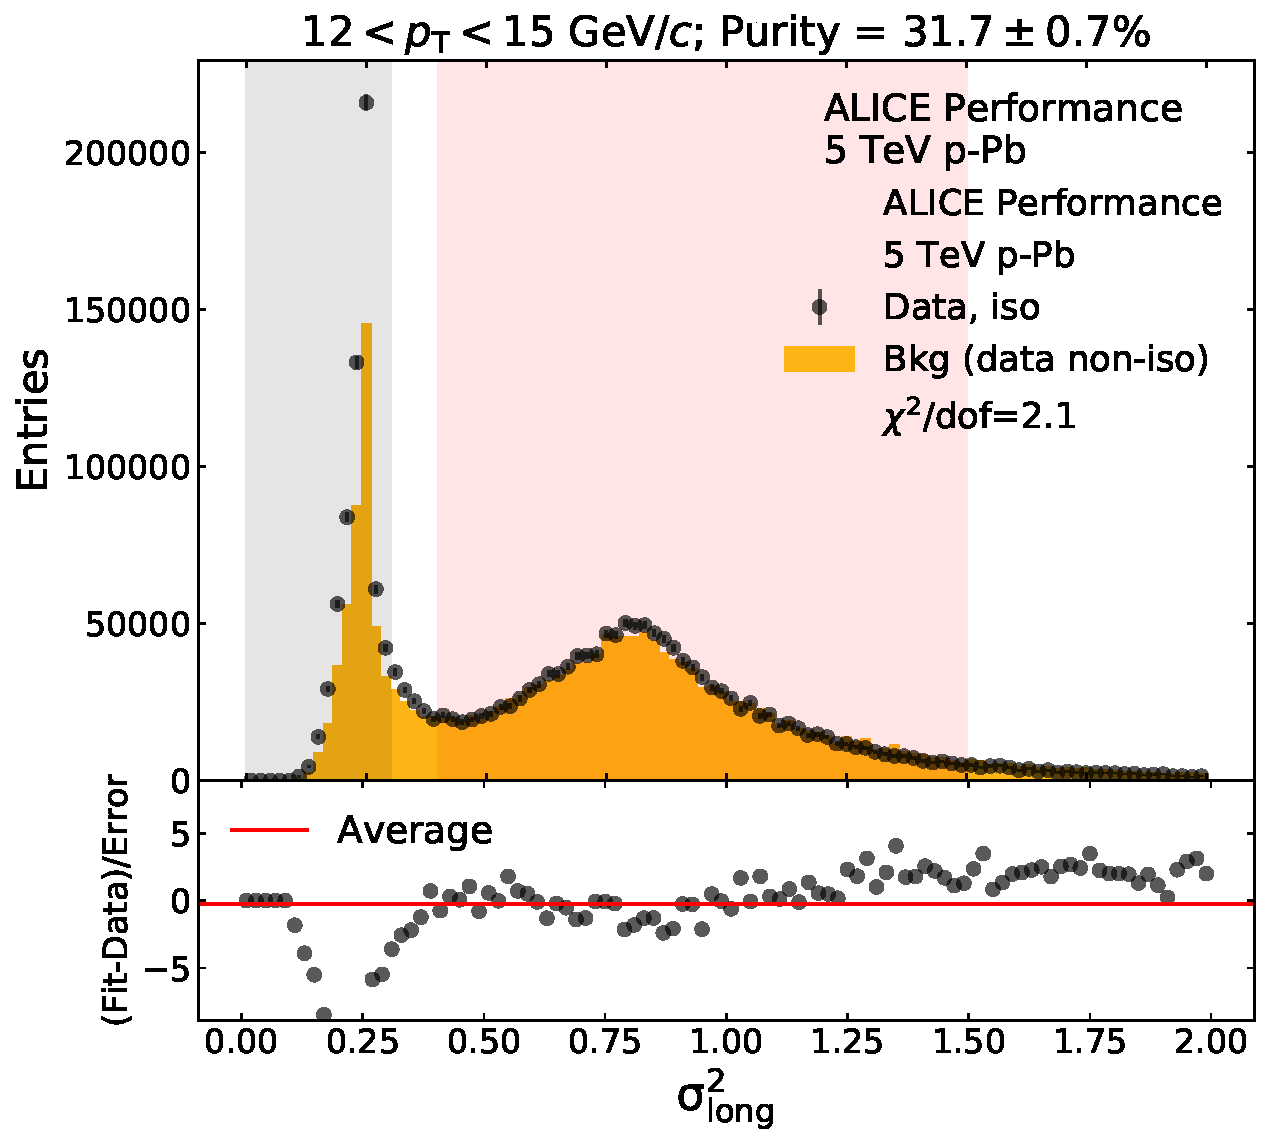
\includegraphics[width=0.38\textwidth]{Purity/bf-example-p-Pb-cluster_Lambda-12-15.pdf}
\\
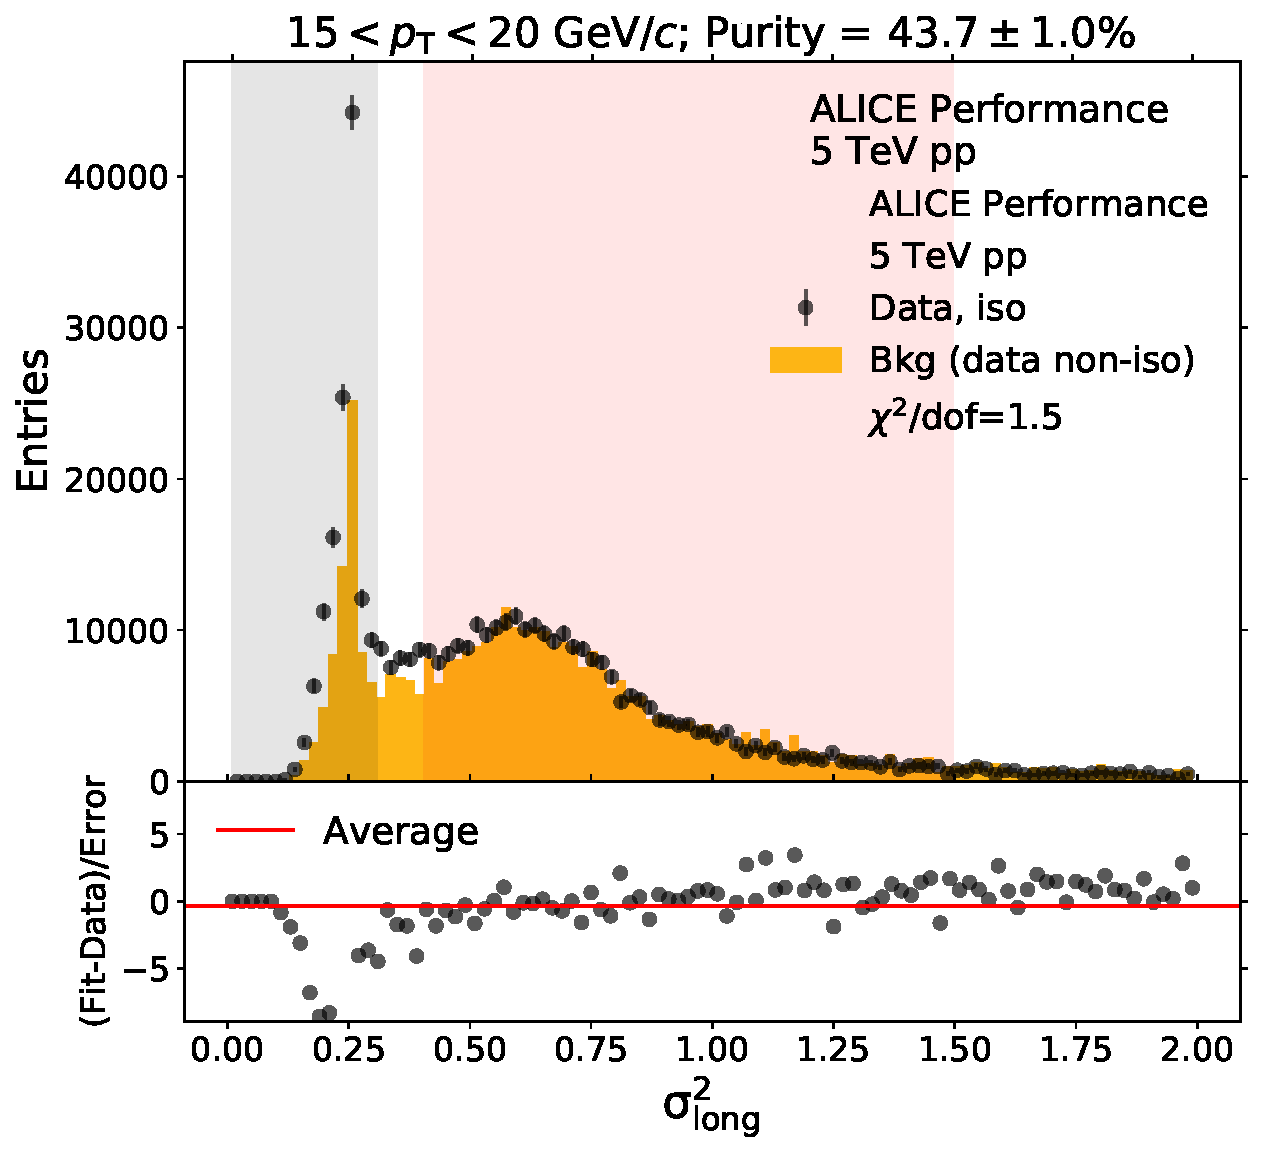
\includegraphics[width=0.38\textwidth]{Purity/bf-example-pp-cluster_Lambda-15-20.pdf}
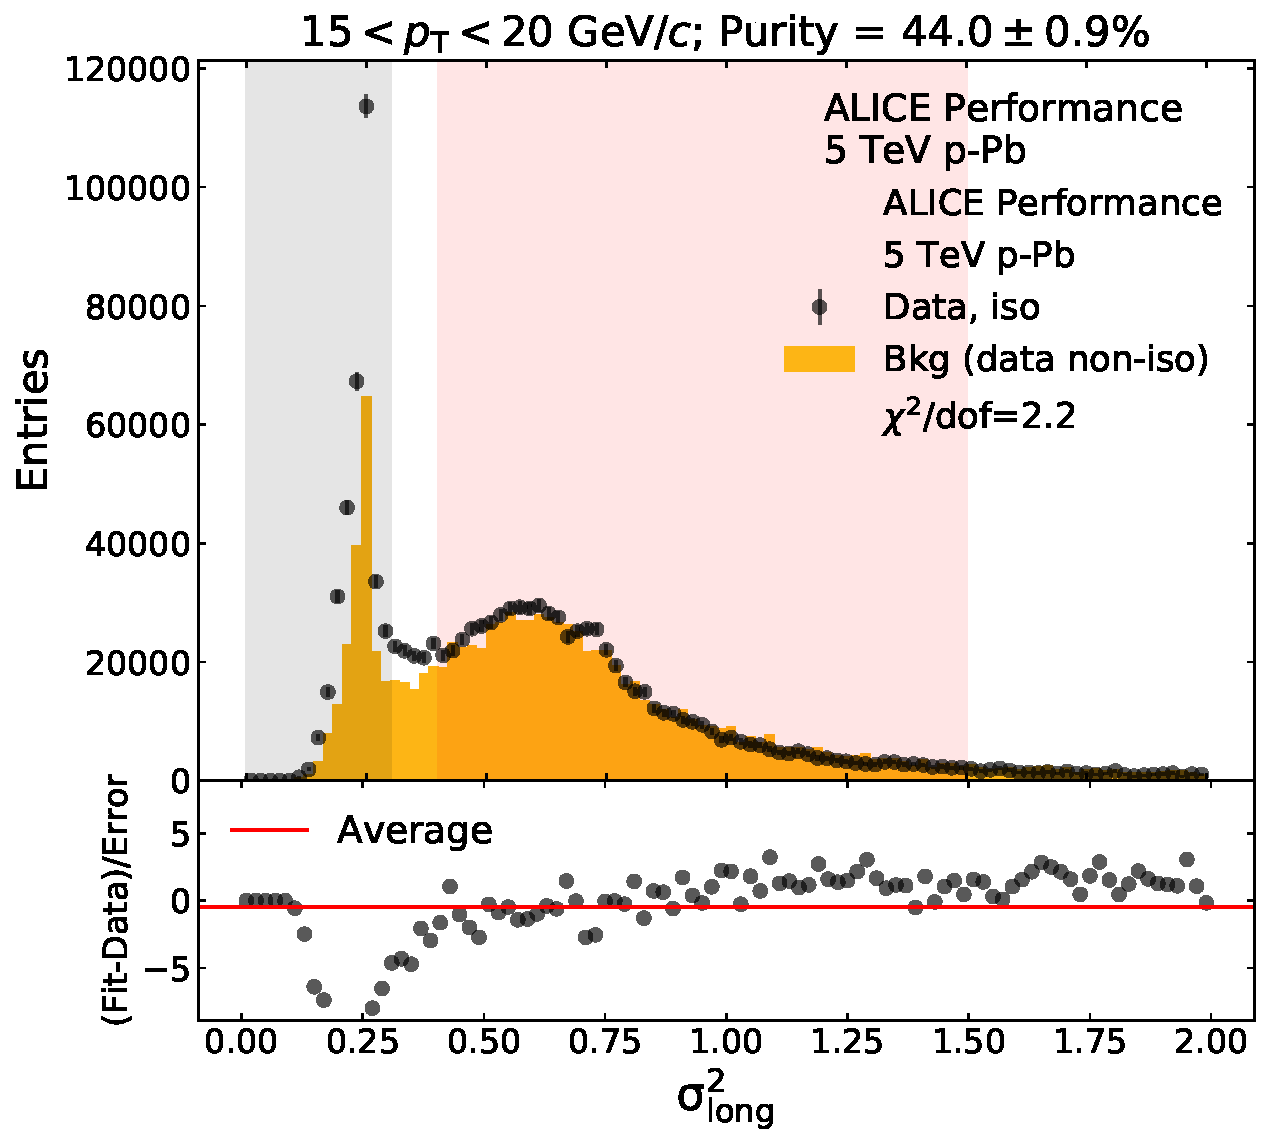
\includegraphics[width=0.38\textwidth]{Purity/bf-example-p-Pb-cluster_Lambda-15-20.pdf}
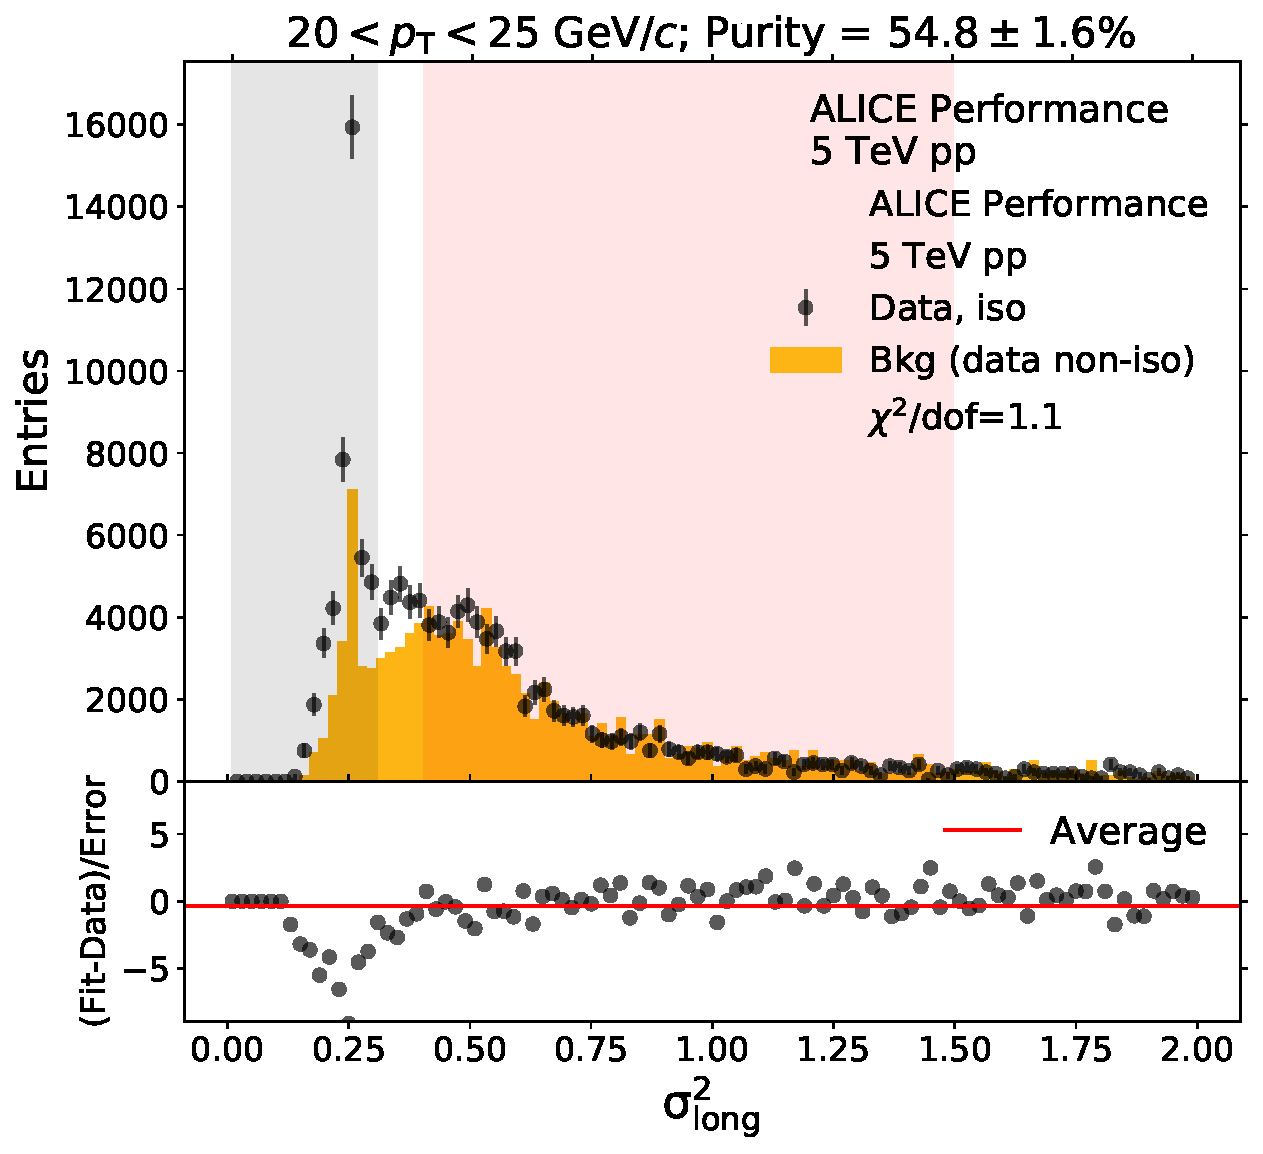
\includegraphics[width=0.38\textwidth]{Purity/bf-example-pp-cluster_Lambda-20-25.pdf}
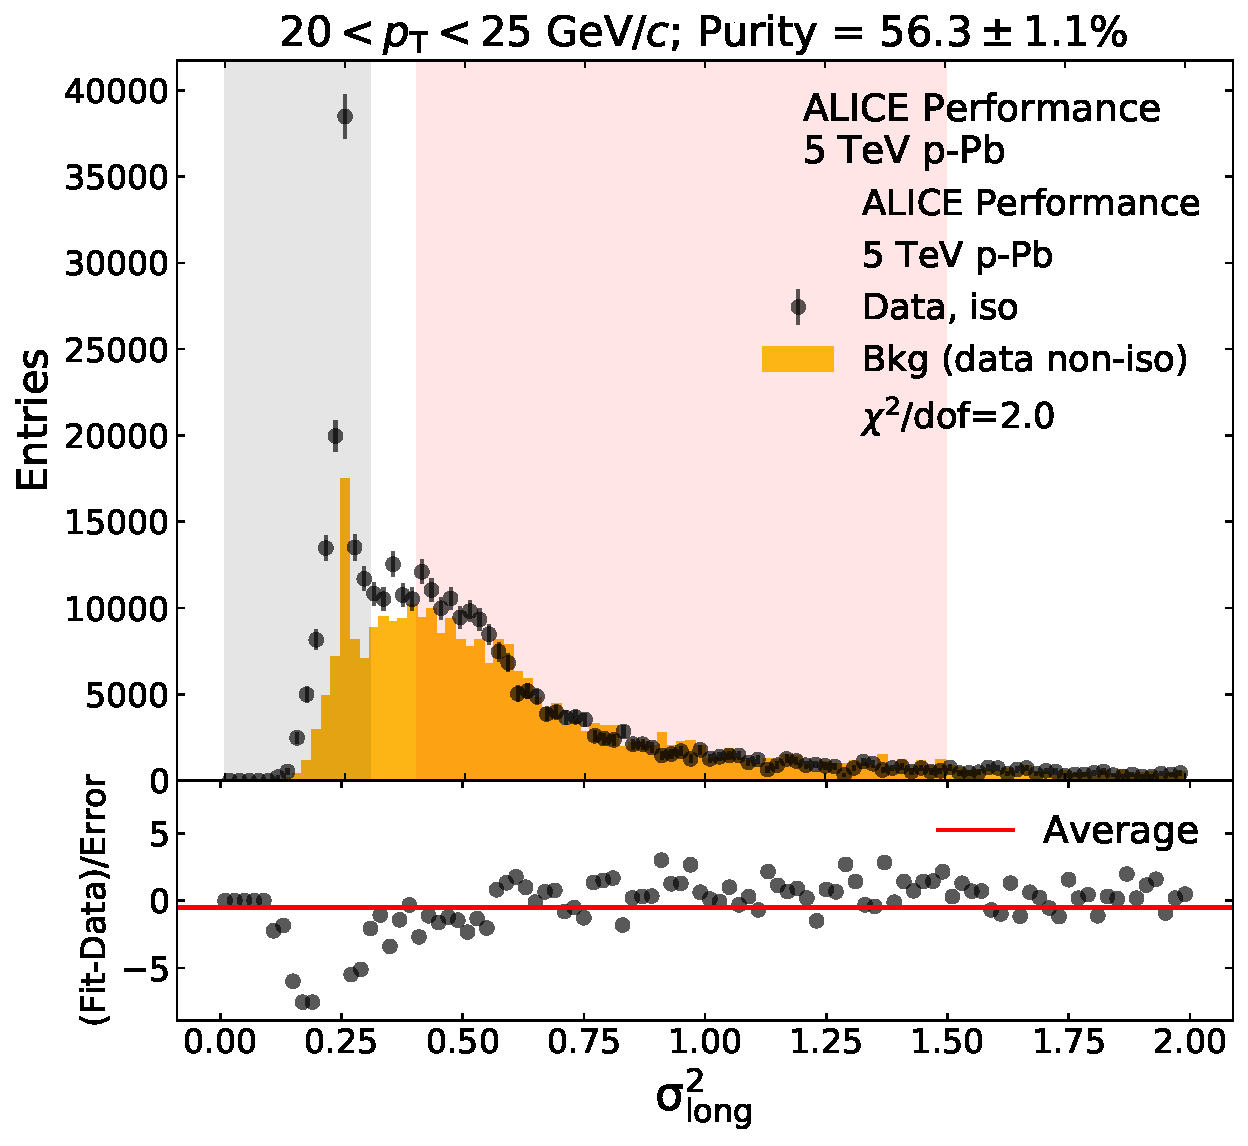
\includegraphics[width=0.38\textwidth]{Purity/bf-example-p-Pb-cluster_Lambda-20-25.pdf}
\\
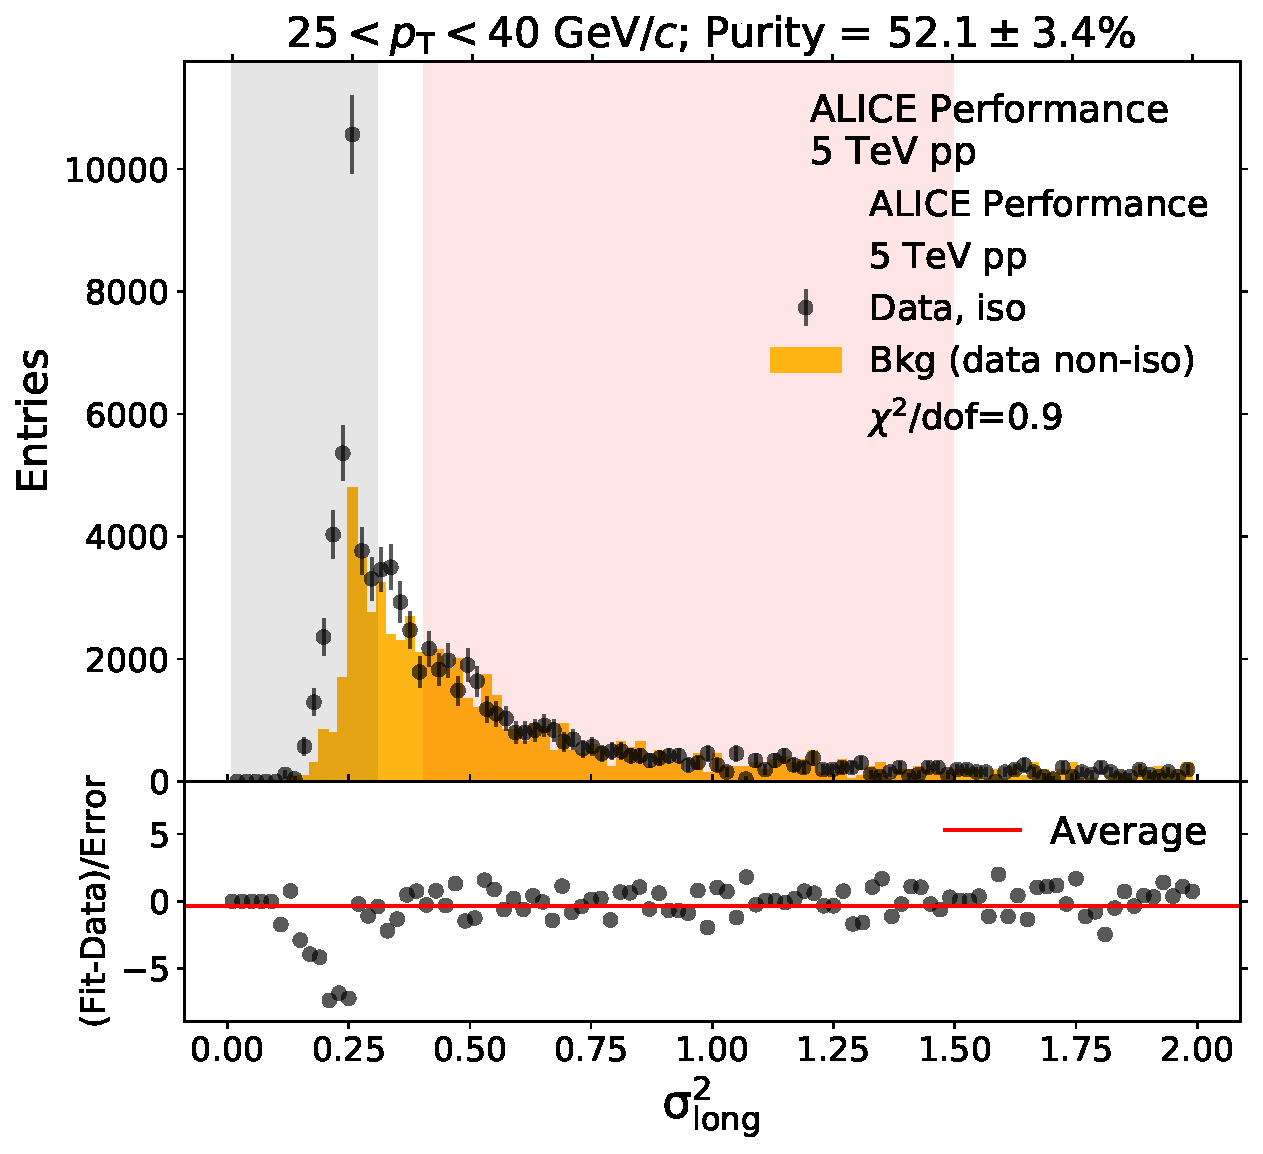
\includegraphics[width=0.38\textwidth]{Purity/bf-example-pp-cluster_Lambda-25-40.pdf}
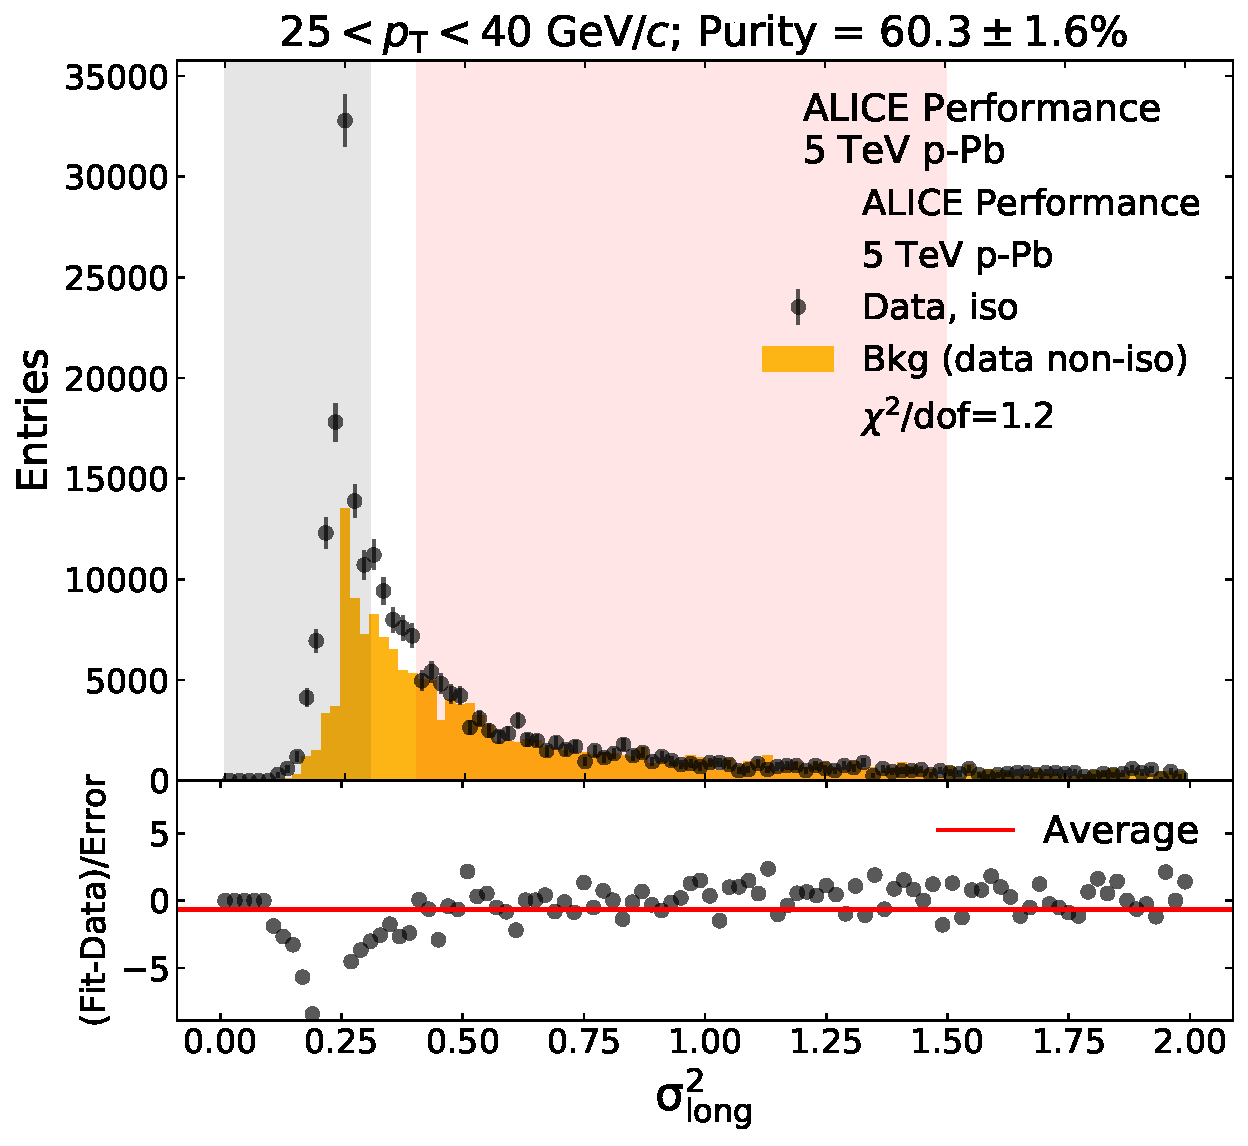
\includegraphics[width=0.38\textwidth]{Purity/bf-example-p-Pb-cluster_Lambda-25-40.pdf}
\caption{Template fit results of background-only template method for pp and \pPb~data. The yellow histograms are the predicted counts given the best-fit value of the total number of clusters in the background dominated region. The hatched gray area represents the interval considered for the purity estimate. The bottom panels show the normalized residuals of the fit, considering the statistical uncertainty on the isolated data and the background template added in quadrature. }
\label{BkgOnlyFit_pPb}
\end{figure}

This method makes the additional assumption that the fraction of signal misclassified as background is small. In a strict sense, this method yields a lower limit on the extracted purity. The results agree with our nominal results within a few percent, indicating that we are not particularly sensitive to the details of the modeling of the shower shape. As a conservative estimate, we take the full difference between our nominal results as a systematic uncertainty in the signal template.

As an additional check, we smear the signal template by multiplying the $\lambdasquare$ of each cluster by a random number selected from a Gaussian with a fixed width before then calculating the purity with this smeared distribution. This was done for a variety of widths up to 10\%, which is much larger than the expected MC simulation mismodelling, and was found to yield a smaller uncertainty than the background-only fit (See Appendix~\ref{sec:smearingsignaltemplate} for more details). Thus, for a final estimate of the systematic uncertainty from the signal template, we take the uncertainty estimated by the background-only fits as described in the previous paragraph.

\FloatBarrier
\subsubsection{Sideband variation in the background template}
\label{sec:bkgtemplate}
To estimate the shower-shape distribution for the $\ydecay$ background in the template fit, a sideband in the cluster isolation variable is used. Only the shape of this distribution is relevant, as the overall background normalization in the signal region (i.e. the purity) is measured with the template fit. As in any analysis using a sideband technique, we nominally use a sideband as close as possible to the signal region and as narrow as possible. Here, we describe how the sideband region is chosen and address the systematic uncertainty that arises from this arbitrary choice.

The cluster isolation distribution is divided into narrow (2 \GeVc) overlapping regions, each of which is used to estimate the background shower-shape distribution. A template fit is performed with each distribution and the $\chi^2$/dof and purity are calculated for each fit and plotted as a function of the anti-isolation region used to create the background template in Figure~\ref{sidebandslices}. Then, the $\chi^2$/dof distribution is examined to determine which regions of anti-isolation result in good fits in the template fit procedure: 5--10 \GeVc~is chosen to be the sideband definition in the final purity calculation.

To calculate the systematic uncertainty on the purity due to this selection, the full range of purities reached by the narrow bands of anti-isolation that fall within 5--10 \GeVc~is considered. Converting the full extent to a systematic uncertainty is a matter of dividing by $\sqrt{12}$ (i.e, the 1 $\sigma$ for a uniform distribution). This results in an absolute uncertainty on the purity of 0.7--5.8$\%$, depending on the collision system and cluster \pt~range.

\begin{figure}[h]
\center
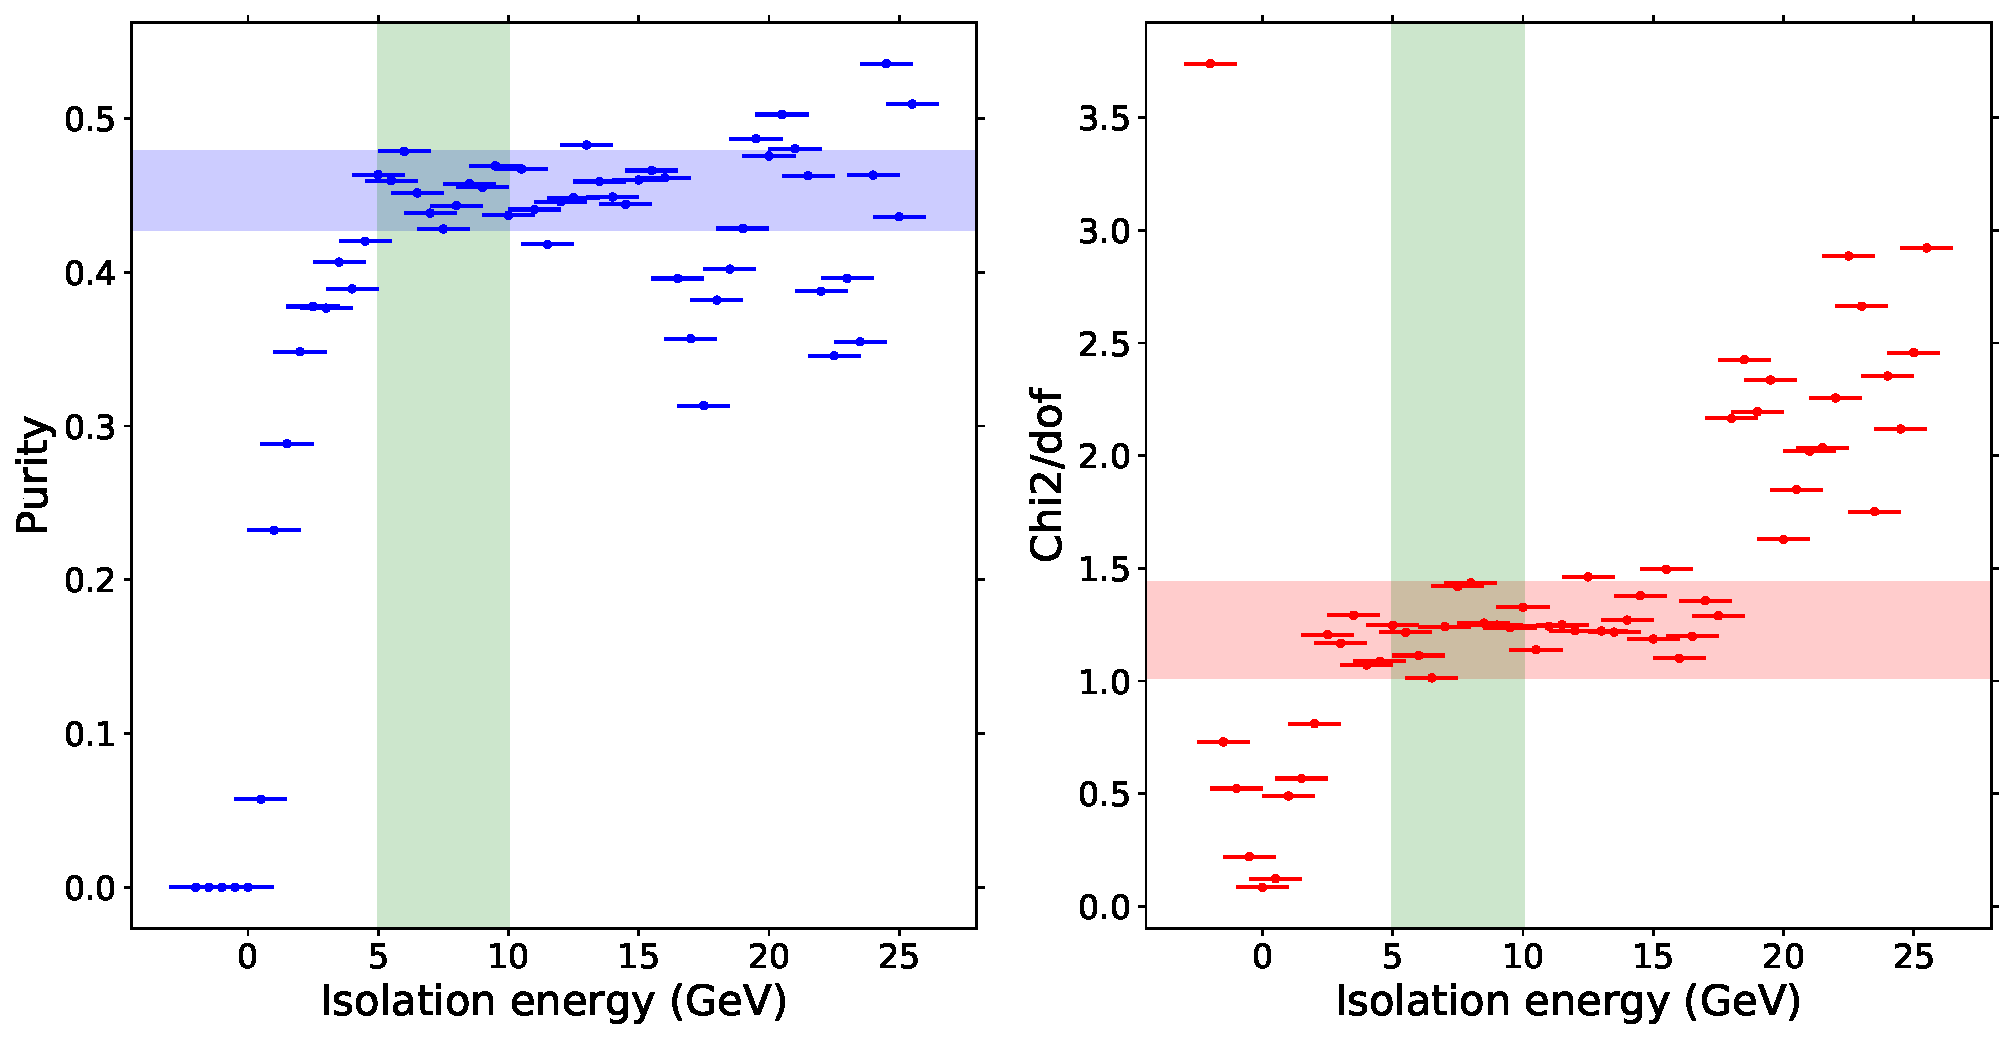
\includegraphics[width=1.0\textwidth]{Purity/antiiso-selection-pp-cluster_Lambda-15-20.pdf}\\
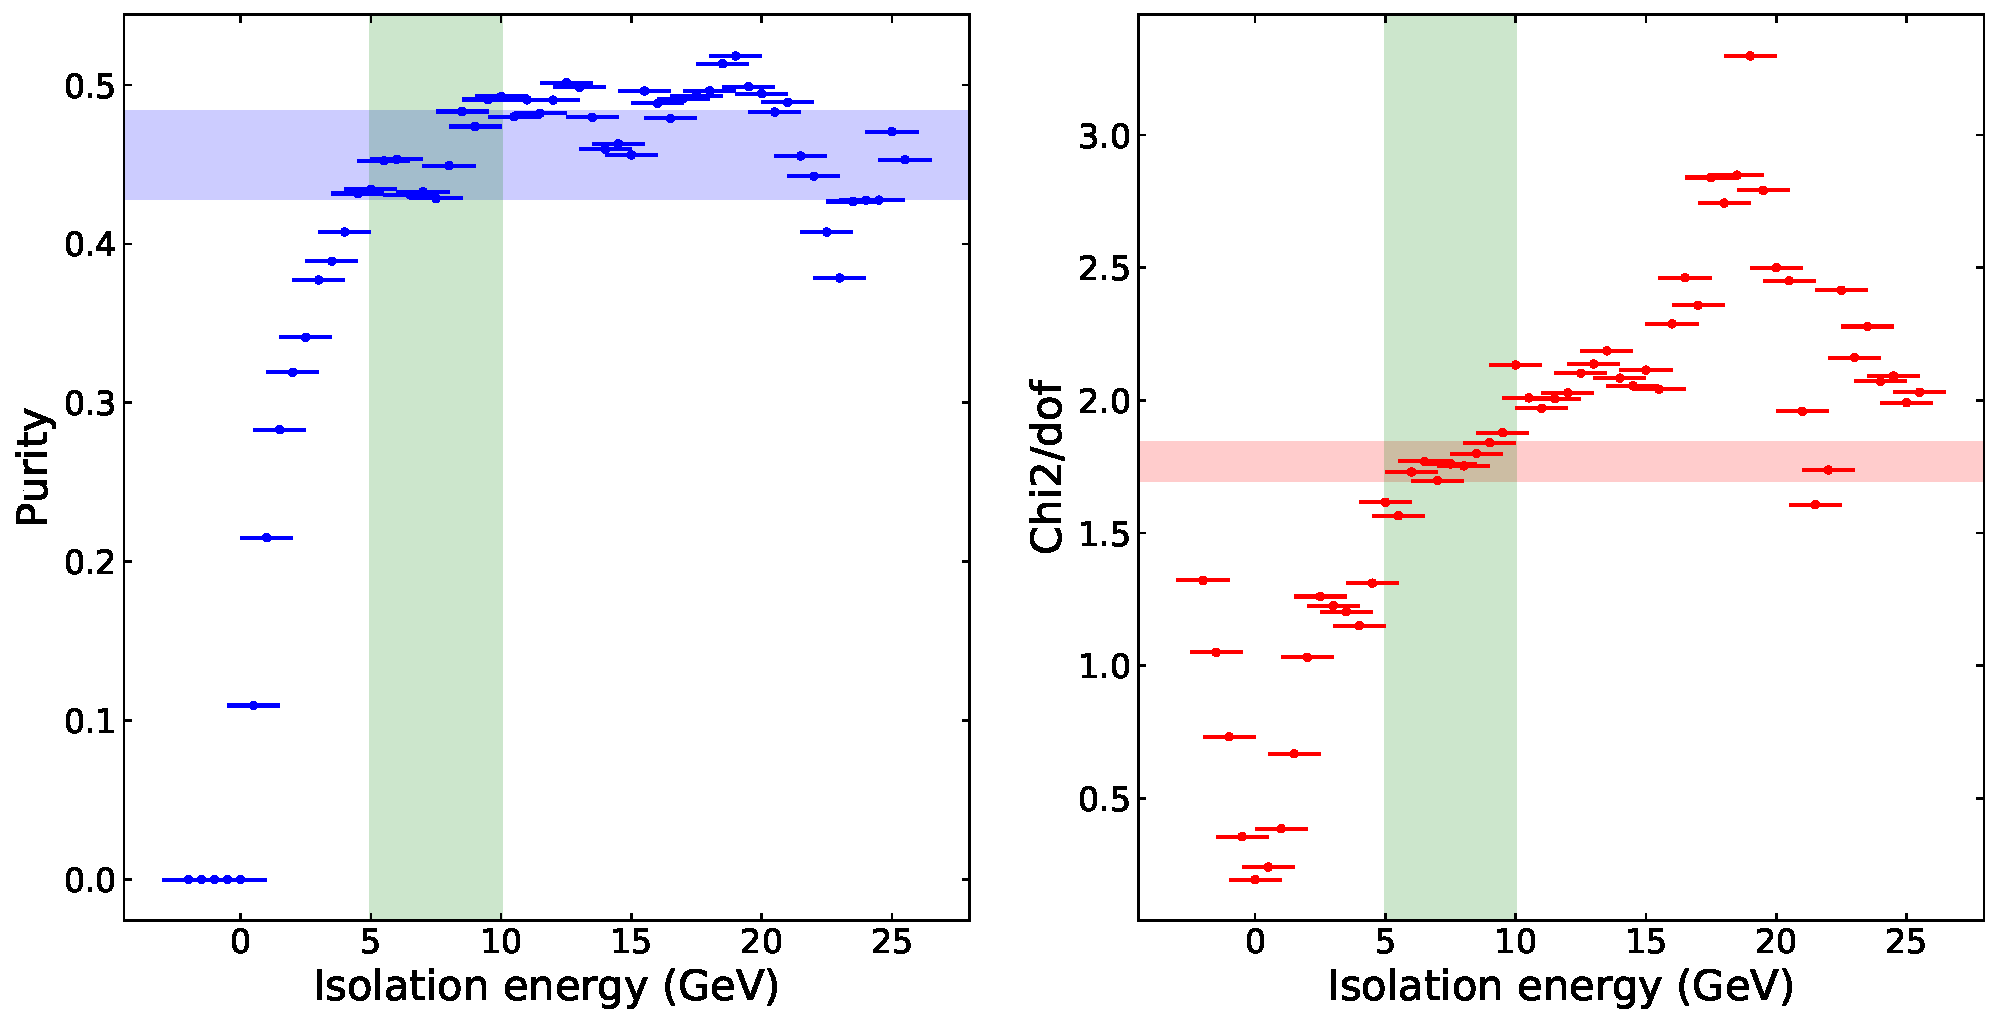
\includegraphics[width=1.0\textwidth]{Purity/antiiso-selection-p-Pb-cluster_Lambda-15-20.pdf}
\caption{Template fit results (purity and $\chi^2$/dof) as a function of anti-isolation region for clusters with $15 < \pt < 20$ \GeVc~in pp (top) and \pPb~(bottom). The green band shows the selected sideband region. The blue and red bands show the full extent of the purity within the selected sideband region.}
\label{sidebandslices}
\end{figure}

\subsubsection{Background template correction}
\label{sec:bkgtemplatecorrection}
Due to the correlation between the isolation and shower shape, the template extracted from the anti-isolated sideband does not exactly reflect the shape of the background in the signal region. Clusters in the isolation sideband have more associated activity than those in the true isolated background and thus emphasize the non-signal region of the shower-shape distribution. Consequently, using the isolation sideband instead of the true isolated background yields systematically higher purities. We note that a similar observation was made for example by the CMS collaboration in their template-fit purity measurements (e.g. Ref.~\cite{Sirunyan:2017qhf})

We correct this bias using a dijet MC simulation, as described in Equation~\ref{eq:bkgtemplatecorrection}. However, this correction is only valid to the extent that the dijet MC reproduces the data. To estimate the systematic uncertainty on this correction, we use a technique based on a method used in the ABCD calculation~\cite{Erwann}. In particular, we use a double ratio to check to which extend does the dijet MC describe the background-dominated region in data: 

\begin{equation}
    \text{Double ratio} = \frac{\text{Iso}_{\text{data}}/\text{Anti-iso}_{\text{data}}}{\text{Iso}_{\text{MC}}/\text{Anti-iso}_{\text{MC}}}
    \label{eq:bkgtemplatedoubleratio}
\end{equation}

In the signal region of the shower shape distribution (0.0--0.3 for $\lambdasquare$), this double ratio will be far from unity, as the data have prompt photons and the dijet MC do not. However, away from that region, where background dominates, the double ratio should be flat (i.e. have no slope) if the dijet MC reproduces the background shower-shape of the data. We note that for this analysis only the shape is important and overall normalization is irrelevant. At a minimum, we expect the variation in the double ratio to be smooth. Thus we fit the double ratio to smooth functions (linear and exponential) in a shower shape range away from the signal region and extrapolate the fit back into the signal region. A similar procedure was used isolated-photon purity measurements with the ABCD method~\cite{Acharya:2019jkx,Erwann}.

Fits to the double ratio are shown in Figures~\ref{fig:bkgtemplatedoubleratiofits_pp} and~\ref{fig:bkgtemplatedoubleratiofits_pPb}, for pp and \pPb~data respectively. We found that the linear and exponential fits gave nearly identical results. In particular, the slope was sufficiently small that the higher-order terms in the exponential were negligible. Thus for the purposes of estimating the systematic uncertainty due to the background template correction, we chose to do only linear fits to the double ratio. In order to remove covariance effects between the slope and intercept, the fits were forced to go through the weighted average of the double ratio value within the fit range at the center of the fit range, making it a single-parameter linear fit with only the slope as a free parameter. This allowed us to propagate the fit uncertainty on the slope to an uncertainty on the purity.


\begin{figure}
    \centering
    \includegraphics[width=\textwidth]{Purity/single-linear-fits-pp}
    \caption{Linear fits for the double ratio (as described in Equation~\ref{eq:bkgtemplatedoubleratio}) for the $\lambdasquare$ variable in pp data.  Included are the value and uncertainty of the fitted slope (in red).}
    \label{fig:bkgtemplatedoubleratiofits_pp}
\end{figure}


\begin{figure}
    \centering
    \includegraphics[width=\textwidth]{Purity/single-linear-fits-p-Pb}
    \caption{Linear fits for the double ratio (as described in Equation~\ref{eq:bkgtemplatedoubleratio}) for the $\lambdasquare$ variable in \pPb~data.  Included are the value and uncertainty of the fitted slope (in red).}
    \label{fig:bkgtemplatedoubleratiofits_pPb}
\end{figure}







These linear fits to the double ratio were done in two fit ranges: 0.5--1.5 and 0.5--1.75 for $\lambdasquare$. In all cases, we found that the slopes were consistent with 0 within the fit uncertainties and thus concluded that that the dijet MC was consistent with the data. Therefore, we did not apply an additional double-ratio correction to the Weights function in Equation~\ref{eq:bkgtemplatecorrection}. We also found that the double ratio fits with the different fit ranges gave purities consistent with each other. So in order to minimize the amount of extrapolation, we did the fit in the largest reasonable fit ranges for each of the variables (the larger of each of the ranges described at the beginning of this paragraph). 

We then took the uncertainty on that double ratio fit and propagated it to a purity uncertainty. This purity uncertainty was then taken to be the systematic uncertainty on the background correction. It varies between 1.2--3.4\% (absolute) depending on cluster \pt~and collision system.


\FloatBarrier
%%%%%%%%%%%%%%%%%%%%%%%%%%%%%%%%%%%%%%%%%%%%%%%%%%%%%%%%%
\subsection{Summary of systematic uncertainties of purity measurement}

Tables~\ref{tab:pursystppblambda} and~\ref{tab:pursystpplambda} give the full estimates of the systematic uncertainties in both collision systems. No single source of systematic uncertainty dominates across \pt~ranges or collision systems.


\begin{table}[h]
    \centering
        \caption{Summary of the systematic uncertainties on the purity as measured with $\lambdasquare$ in \pPb~collisions. All values are in absolute percentage. ``Stat.'' refers to the statistical uncertainty; ``Signal'' refers to the signal template uncertainty; ``Anti-iso'' refers to the uncertainty due to the sideband selection; ``Bkg'' refers to the uncertainty due to the background template correction; ``Total'' is the sum of the previous three columns in quadrature.}
    \begin{tabular*}{1.0\columnwidth}{@{\extracolsep{\fill}}lcccccc@{}}
    \hline
    	pT(GeV/$c$) & Purity & Stat. & Signal & Anti-iso & Bkg & Total syst \\ \hline
    	12.0-15.0 & 20.7 & 1.1 & 1.1 & 0.8 & 1.5 & 2.0 \\
    	15.0-20.0 & 34.2 & 1.2 & 2.0 & 1.6 & 1.2 & 2.8 \\
    	20.0-25.0 & 47.6 & 1.7 & 1.9 & 1.1 & 1.7 & 2.7 \\
    	25.0-40.0 & 54.6 & 1.8 & 2.3 & 2.4 & 2.1 & 3.9 \\
    \end{tabular*}
    \label{tab:pursystppblambda}
\end{table}


\begin{table}[h]
    \centering
        \caption{Summary of the systematic uncertainties on the purity as measured with $\lambdasquare$ in pp collisions. All values are in absolute percentage. ``Stat.'' refers to the statistical uncertainty; ``Signal'' refers to the signal template uncertainty; ``Anti-iso'' refers to the uncertainty due to the sideband selection; ``Bkg'' refers to the uncertainty due to the background template correction; ``Total'' is the sum of the previous three columns in quadrature.}
    \begin{tabular*}{1.0\columnwidth}{@{\extracolsep{\fill}}lcccccc@{}}
    \hline
    	pT(GeV/$c$) & Purity & Stat. & Signal & Anti-iso & Bkg & Total syst \\ \hline
    	12.0-15.0 & 20.1 & 1.7 & 2.0 & 1.2 & 2.9 & 3.7 \\
    	15.0-20.0 & 31.7 & 2.0 & 2.5 & 1.5 & 2.4 & 3.8 \\
    	20.0-25.0 & 47.3 & 2.9 & 0.8 & 3.0 & 2.8 & 4.2 \\
    	25.0-40.0 & 48.5 & 3.5 & 5.9 & 4.0 & 3.4 & 7.9 \\
    \end{tabular*}
    \label{tab:pursystpplambda}
\end{table}


%[I have commented out, it is redundant]
%An overall summary of the purity, statistical uncertainty, and total systematic uncertainty in pp and \pPb~datasets is given in Table~\ref{tab:puruncertaintypp}.

%\begin{table}[h]
%	\centering
%		\caption{Summary of purities and statistical and systematic uncertainties for pp and \pPb~collisions. All values are absolute percentages.}
    % \begin{tabular*}{1.0\columnwidth}{@{\extracolsep{\fill}}l|ccc|ccc@{}}
    % 	\hline
    % 	 & \multicolumn{3}{c|}{pp} & \multicolumn{3}{c}{p-Pb} \\ \hline
    % 	pT(GeV/$c$) & \lambdasquare & $\sigma_{\text{stat}}$ & $\sigma_{\text{syst}}$ & \lambdasquare & $\sigma_{\text{stat}}$ & $\sigma_{\text{syst}}$ \\ \hline
    % 	12.0--15.0 & 20.1 & 1.7 & 3.7 & 20.7 & 1.1 & 2.0 \\
    % 	15.0--20.0 & 31.7 & 2.0 & 3.8 & 34.2 & 1.2 & 2.8 \\
    % 	20.0--25.0 & 47.3 & 2.9 & 4.2 & 47.6 & 1.7 & 2.7 \\
    % 	25.0--40.0 & 48.5 & 3.5 & 7.9 & 54.6 & 1.8 & 3.9 \\
    % 	\hline
    % \end{tabular*}
%	\label{tab:puruncertaintypp}
%\end{table}

%\subsubsection{Data-driven shower shape with eta decays}
%We study the shower-shape distribution for single photons from data by using $\eta$ decays obtained in the 13 %TeV pp data collected in 2016 and 2017. Pairs of photons with an invariant mass consistent with a $\eta$ decay are used. The signal-to-noise ratio is about XX. The background is estimated by using a two-sided sideband around the $\eta$ peak. The shower-shape distributions for photons with $p_{T}>8 $ GeV is shown in Figure~\ref{ShoweShape} and is compared with the distribution obtained from sgamma--jet .  The simulation is weighted such that it matches the $p_{T}$ distribution measured in the data. 
%\begin{figure}
%\center
%\includegraphics[width=0.95\textwidth]{Purity/EtaShowerShape}
%\caption{Data-driven shower shape (left panel is DNN and right panel lambda) distribution with photons from %$\eta$ decays. The simulation was weighted to reflect the $p_{T}$ distribution obtained in data}
%\label{ShoweShape}
%\end{figure}

%The comparison shows that the simulation is consistent with the data-driven distribution, within statistical uncertainties. 


%Figure~\ref{SignalShowerShapes} shows the distribution of the shower-shape variables for photon-jet simulation of pp collisions. The $\lambdasquare$ variable peaks at 0.25 and is mostly symmetric but has a small tail to larger values. The DNN variable shows a relatively broad peak at {DNN$\approx0.75$}, and a tail to lower values.
% The $\emax$ variables reveals that for most of the signal clusters the seeding cell contains about 75--85$\%$ of the total cluster energy, but the distribution has a pronounced tail that extends to values as low as 50$\%$ and an even smaller tail that reaches 25$\%$. 

%\begin{figure}[h]
%\center
%\includegraphics[width=1.0\textwidth]{Purity/ShowerShapeVariables}
%\caption{Shower shape distributions, from photon-jet simulation, of clusters with {$12<\pt<16$ GeV}.}
%\label{SignalShowerShapes}
%\end{figure}

%The shape of the distributions shown in Figure~\ref{SignalShowerShapes} reveal that not all the shower shapes from signal photons are similar (as a naive look at the $\lambdasquare$ peak would led us to believe). This is to be expected, as some photons hit near the center of a cell and the shower is contained in mostly one cell, while others hit near the boundary of cells, or hit at a slight angle due to the ``approximate protectiveness" of the EMCal/DCal system.

%FigureTemplatefitResults_pp shows fit results in p-Pb and pp data. In both cases, a good fit with no systematic pattern in the residuals is achieved over most of the distribution, with reduced $\chi^{2}$ in the 1.0--2.7 range. 
%The systematic variation of the residuals of the $\lambdasquare$ fit is attributed to the very sharp peak of this distribution. We do not attempt to further improve the fit quality but instead take these as part of our systematic uncertainties. In Section~\ref{sec:puritysystematics}, we also present results without a signal template. %The results show a signal fraction of about 10--13$\%$, integrated over the entire shower shape distributions. The purity is determined as the fraction to background after the shower shape cut that is used in the $\gammaiso$ selection (DNN$>0.55$ or $\lambdasquare<0.4$)

%\FloatBarrier
%\subsection{Consistency check with photon spectra}
%We perform a check on the purity and efficiency obtained with different shower-shapes on the number of prompt photons that pass our selection. The check is performed by correcting the spectrum of prompt photons passing the cuts by the cut efficiency and purity. The resulting spectra are then compared with one another. 
%The photon spectrum is a physical quantity that should be independent of the shower-shape cut used, so it allows us to cross-check the purity and shower-shape cut efficiency corrections. 

%Figure~\ref{fig:ShowerShapeEfficiency} shows the shower-shape cut efficiency. The $\lambdasquare<0.3$ and the DNN$>0.75$ selections yield similar efficiencies of about 80$\%$ with only a mild $\pt$ dependence.

%\begin{figure}[h]
%\center
%\includegraphics[width=0.495\textwidth]{Purity/ShowerShapeEfficiency_Skimmed_13def_root}
%\includegraphics[width=0.495\textwidth]{Purity/ShowerShapeEfficiency_Skimmed_17q_root}
%\caption{Shower-shape cut efficiency as a function of cluster $\pt$ obtained from photon+jet simulations in p-Pb (left) and pp (right). The statistical uncertainty in the measurement is smaller than the marker size.}
%\label{fig:ShowerShapeEfficiency}
%\end{figure}

%Figure~\ref{fig:ConsistencywithSpectra} shows the results of the check in p-Pb and pp data. The obtained spectra are consistent within $15--20\%$ of the average over the momentum range measured. 

%\begin{figure}[h]
%\center
%\includegraphics[width=0.495\textwidth]{Purity/Spectra_Skimmed_13def_root}
%\includegraphics[width=0.495\textwidth]{Purity/SpectraRatio_Skimmed_13def_root}\\
%\includegraphics[width=0.495\textwidth]{Purity/Spectra_Skimmed_17q_root}
%\includegraphics[width=0.495\textwidth]{Purity/SpectraRatio_Skimmed_17q_root}
%\caption{Left panel: Number of isolated prompt photons as a function of transverse momentum obtained with different shower-shape selections. The error bars represent statistical uncertainty only. Right panel: Ratio to average. The grey band represents $\pm$15$\%$ around unity.}
%\label{fig:ConsistencywithSpectra}
%\end{figure}

%\begin{figure}[h]
%\center
%\includegraphics[width=0.495\textwidth]{Purity/PurityRatioSkimmed_17q_root.pdf}
%\includegraphics[width=0.495\textwidth]{Purity/PurityRatioSkimmed_13def_root.pdf}
%\caption{Ratio of the purity of different shower-shape variables to the purity of $\sigma_\mathrm{long}^{2}$ as a function of cluster transverse momentum.The plot on left is for pp photon-triggered data and the plot on the right is for p-Pb photon-triggered data. The grey band represents $\pm$ 5$\%$ around unity. The error bars consider only statistical uncertainties.}
%\label{fig:purityratio}
%\end{figure}

%In this section, we describe how we estimate the systematic uncertainty associated with our background template. We describe the sensitivity of our template fits to variations of the sideband region limits in Section~\ref{sec:sidebandvariation} and checks with simulation in Section~\ref{sec:checkwithMC}.

%\begin{figure}
%\center
%\includegraphics[width=1.0\textwidth]{Purity/IsolationCorrelationSkimmed_13def_root}\\
%\includegraphics[width=1.0\textwidth]{Purity/IsolationCorrelationSkimmed_17q_root}
%\caption{Shower shape distributions for different anti-isolation sideband regions in pp (upper row) and p-Pb data (bottom row).}
%\label{SidebandVariation}
%\end{figure}

%Figure~\ref{SidebandVariation} shows that there is no strong dependence of the shower-shape distributions on the variations of the sideband definition, until one reaches a large value of the anti-isolation cut. This illustrates in a different way the result already shown in Figure~\ref{sidebandslices}. 

%\begin{figure}[h]
%\center
%\includegraphics[width=0.49\textwidth]{Purity/bf-example-pp-cluster_NN1-12-14redbin.pdf}
%\includegraphics[width=0.49\textwidth]{Purity/bf-example-pp-cluster_NN1-20-25redbin.pdf}
%\caption{Representative fit results of background-only template method for pp data using the using the DNN and $\lambdasquare$ variables. The yellow histograms are the predicted counts given the best-fit value of the total number of clusters in the background dominated region. The hatched gray area represents the interval considered for the purity estimate. The bottom panels show the normalized residuals of the fit, considering the statistical uncertainty on the isolated data and the background template added in quadrature. }
%\label{BkgOnlyFit_pp}
%\end{figure}

%\begin{figure}[h]
%\center
%\includegraphics[width=1.0\textwidth]{Purity/bkg-template-iso-vs-antiiso.pdf}
%\caption{Background simulation of the shower-shape distributions in the signal and sideband regions for clusters with $12<\pt<30$ \GeVc.}
%\label{BKGshape}
%\end{figure}

%Figure~\ref{Erwanns} shows the purity results obtained with the ABCD method with charged only and charged + neutral energy. The results show that the purity increases, as expected, but the increase is only about $10\%$ in the range 10--16 \GeVc~and about 5$\%$ between 20--30 \GeVc. 

%\begin{figure}[h]
%\center
%\includegraphics[width=1.0\textwidth]{Purity/ErwannsSlide}
%\caption{Purity results obtained with the ABCD method with charged+neutral (left) and charged-only (right) isolation for the 2013 p-Pb data. From slides presented by E. Masson during the Physics forum in 04/24/18. }
%\label{Erwanns}
%\end{figure}

%\subsection{Comment on neutral energy in isolation}
%\label{sec:neutraliso}
%In principle, we could expand the definition of our isolation variable to include energy measured in the calorimeters. This has been studied in the context of spectra analysis with 2013 p-Pb data~\cite{Erwann}. 

%However, the associated biases from stronger correlation between the shower-shape variable and isolation variable (needed for the purity measurements) increases for $\pi^{0}$ decays. This is visible in the results shown in the figure, especially at lower momentum, where it is less likely for a $\pi^{0}\to\gamma\gamma$ to produce a merged cluster. The correction factor is higher, as can be observed in the figure. Based on this study, we do not pursue studies on the inclusion of neutral energy in the isolation energy. A quantitative comparison of purities from the template fit and ABCD method is presented in Section~\ref{sec:comparisontoABCD}.

%This section describes the systematic uncertainty associated with our purity measurement. We estimate this independently for each shower-shape variable. As described in Section~\ref{sec:systematics}, for our final analysis we use the variables separately and estimate the uncertainty due to shower-shape definition in the final $\gammaiso$--hadron and $\gammaiso$--jet results.

%The measured purity values is compatible within a given data set and between pp and \pPb~datasets. The fact that the pp and \pPb~purities agree is not surprising given the fact that they are driven by the EMCal granularity and the $\gamma_{\mathrm{prompt}}/\pi^{0}$ cross-section ratio, which are likely very similar in both datasets. This also shows that the larger underlying event in \pPb~is appropriately subtracted; otherwise, the resulting purity would have been significantly lower due to improper UE subtraction. 

%Figure~\ref{fig:Chi2} shows the reduced $\chi^{2}$ for all the fit results presented in Table~\ref{tab:purity}. This shows than an acceptable goodness-of-fit is achieved for all the \pt~intervals considered. 

%\begin{figure}[h]
%\center
%\includegraphics[width=0.495\textwidth]{Purity/combinedupdated.pdf}
%\caption{Reduced $\chi^{2}$ of template fit as a function of cluster $\pt$ for pp and \pPb~data.}
%\label{fig:Chi2}
%\end{figure}
\FloatBarrier
\section{Tracking}
\label{sec:tracking}
This section describes the performance of ITS-only tracking. During the 13def and 17q periods, the TPC was either not read out or compromised due to space-charge distortions so we rely on only the ITS for track reconstruction. Thus the purpose of this section is to demonstrate that we can use ITS-only tracking to measure tracks up to relatively large track $\pt$.

Our strategy is to measure the charged-particle $\pt$-spectrum using ITS-only tracking and to compare it with the normal TPC+ITS tracking in the data-taking period when the TPC was active and free of space-charge distortions (i.e. the low-luminosity 13b data-taking period of 5 TeV \pPb~minimum-bias data) and with published ALICE measurements~\cite{Acharya:2018qsh} that use the same dataset. By comparing to published measurements in the same system and center-of-mass energy, we avoid any ambiguity related to the reference spectrum. 

Our aim is to validate the combined effect of tracking efficiency, fake rate, and track momentum smearing corrections that are based on MC simulations. We also rely on this study to estimate systematic uncertainties due to mis-modeling of the tracking performance. So, in effect, we are performing a cross-calibration or bootstrapping with the standard ALICE tracking.

For this study, we use minimum bias \pPb~events for both data and Monte Carlo. The Monte Carlo simulations used for this section are LHC13b2\_efix\_p1, which a \textsc{DPMJET} anchored to LHC13b,c and LHC17l3b, which is a pp \textsc{Pythia8}, anchored to LHC17p. The data used runs from LHC13b. The \pPb~data sets match the ones used in the published ALICE measurements mentioned previously. 

For this tracking performance analysis, we  only use events with the minimum bias trigger (CINT7). We also apply the vertex and pileup selections described in Section~\ref{sec:eventselection}. The tracks reconstructed from the ITS (``ITS-only tracks"), are compared with tracks reconstructed from information obtained from both the TPC and ITS (``TPC+ITS tracks"). Here, ITS-only tracks are really reconstructed in a standalone way and are not simply the ITS-segment of a ITS+TPC track.~\footnote{The standalone ITS-only tracks can be retrieved from ESD data by demanding a track status of `` \textsc{AliESDtrack::kITSPureSA}''. The exact line in the code is a follows: \textit{        \_track\_cut.back().SetRequireITSPureStandAlone(kTRUE);}.}

In order to select good-quality tracks emerging from the primary vertex while maintaining a high efficiency, each track is required to satisfy the cuts summarized in Table~\ref{tab:track_cuts}. A set of standard PWG-JE cuts are applied to all tracks, and additional track cuts are applied depending on whether the track is a TPC+ITS track or an ITS-only track. 
\begin{table}[h]
   \centering
      \caption{Summary of the cuts used in Track Selection.}	
   \label{tab:track_cuts}
   \begin{tabular*}{1.0\columnwidth}{@{\extracolsep{\fill}}l|c@{}}
      	\hline
 		\textbf{Common Cuts}\\
        %\textbf{ITS--Only Cuts}\\
        \hline
        track $\eta$ & $|\eta| < 0.8$\\
        track $\pt$ & $\pt \geq 0.150$ \GeVc\\
        SetMaxDCAToVertexXY & 2.4 cm\\
        SetMaxDCAToVertexZ & 3.2 cm\\
        SetDCAToVertex2D & TRUE\\
		\hline \hline
        \textbf{TPC+ITS Cuts}\\
        \hline
        SetMinNClustersTPCPtDep & 70.+30./20.*x, 20.0\\ 
        SetMinNClustersTPC & 70\\
        SetMaxChi2PerClusterTPC & 4\\
        SetMaxChi2PerClusterITS & 36\\
        SetMaxFractionSharedTPCClusters & 0.4\\
        SetMaxChi2TPCConstrainedGlobal &36 \\
        SetRequireTPCStandAlone & TRUE\\
        SetRequireTPCRefit & TRUE \\
        SetRequireITSRefit & TRUE\\
        SetRequireSigmaToVertex & FALSE \\
        SetAcceptKinkDaughters & FALSE\\
        \hline \hline
        \textbf{ITS--Only Cuts}\\
        \hline
        SetRequireITSPureStandAlone &TRUE\\
        SetMinNClustersITS & 4\\
        SetMaxChi2PerClusterITS & 36\\
        \hline
   \end{tabular*}
\end{table}
\FloatBarrier
\subsection{Tracking performance with and without TPC}
\label{sec:closurewithdata}
Our strategy to validate the use of ITS-only tracking relies on cross-calibration with the normal TPC+ITS tracking and comparisons with published data. To this end, we first measure a charged-particle $\pt$ spectrum using TPC+ITS reconstruction to reproduce the published data and thus demonstrate the validity of our method. We then repeat the measurement with ITS-only reconstruction and compare the results.

The method we use contains the following steps: 
\begin{enumerate}
\item Using the MC simulations, obtain the efficiency, the fake rate, and a track-$\pt$ response matrix.
\item Obtain a $\pt$ spectrum from the minimum-bias data with either ITS-only or TPC+ITS tracking. 
\item Apply a $\pt$-dependent fake rate correction to the spectra of point 2. 
\item Multiply the published spectrum by the track efficiency. 
\item Finally, use the response matrix to smear the result of point 4.
\item Compare the result of point 5 with the result of point 3. 
\end{enumerate}

If the efficiency, fake rate, and response matrix, which are all obtained from MC simulations, faithfully represent the tracking performance of the data, then it follows that the result of point 3 should be compatible with the result of point 5. We use this fact to constrain the degree to which mis-modeling of the detector response could affect single-track $\pt$ spectra.

Note that we could have attempted to directly measure a charged-particle spectrum, applying an efficiency correction to the result of point 3 and then unfolding that result. That would have been directly comparable to the published data. However, the systematic uncertainties intrinsic to the unfolding procedure would result in relatively large systematic uncertainties, but these are unrelated to the issue we discuss here. 

We note that using the response matrix to smear the published data is a mathematically well-defined procedure (as opposed to unfolding, which requires an inversion of the response matrix subject to the statistical uncertainties of the data). Given that our aim is to test the corrections and response matrix in a robust and unambiguous way, we follow the above steps to avoid unfolding systematic uncertainties.

\subsubsection{Efficiency and fake rates}
\label{sec:Efficiency_fake_rates}
%The tracking efficiency is calculated from the minimum bias \pPb~simulation (see Table~\ref{tab:MCsamples}).
The tracking efficiency is defined as the ratio of the number of reconstructed primary particles\footnote{No special tuning of the particle type composition is performed. This typically only matters at low $\pt$ and enforces a small (percent level) correction to the out-of-the-box results.}, $N_{\mathrm{prim,rec}}(p_\mathrm{T})$, to the number of generated primary particles, $N_{\mathrm{prim,gen}}$. The truth-to-reconstructed matching is done following the standard ALICE method\footnote{The information is retrieved with the method ``track$\to$GetLabel()".}. Thus, the efficiency is defined as: 
\begin{equation}\label{eq:eff}
\epsilon (\pt^{\mathrm{true}}) = \frac{N_{\mathrm{prim,rec}}(\pt^{\mathrm{true}})}{N_{\mathrm{prim,gen}}(\pt^{\mathrm{true}})}.
\end{equation}

As the equation suggests, we use the simulated or ``truth'' transverse momentum, $\pt^{\mathrm{true}}$, for both the numerator and denominator in our efficiency. This way, we factorize out effects of efficiency from bin-migration due to momentum smearing.

The numerator of Equation~\ref{eq:eff} is restricted for charged particles with generated pseudorapidity in the range $|\eta^{\mathrm{true}}|<0.8$ and azimuth $0<\varphi^{\mathrm{true}}<2\pi$. Therefore, the correction factor accounts for both geometrical acceptance, detector inefficiencies, and dead channels.  

Fake tracks are defined as reconstructed tracks that do not match to a truth, primary particle. The fake rate is determined by taking a ratio of the number of fake tracks to the total reconstructed tracks and is parametrized as a function of the reconstructed transverse momentum of the track, $\pt^{\mathrm{reco}}$:

\begin{equation}\label{eq:fakes}
\mathrm{fake rate} (\pt^{\mathrm{reco}}) = \frac{N_{\mathrm{unmatched}}(\pt^{\mathrm{reco}})}{N_{\mathrm{all reco}}(\pt^{\mathrm{reco}})}.
\end{equation}

Figure~\ref{fig:tpcEff} shows the efficiency and the fake rates for the TPC+ITS and ITS only tracks. In both cases the efficiency grows with $\pt$ up to about 1 \GeVc~where it dips and it reaches a plateau value with no significant $\pt$ dependence. The efficiency starts at about 57$\%$ for the TPC+ITS tracks and at 70$\%$ for ITS-only tracks at 150 MeV and plateaus at 84\% and 88\% respectively. %The plateau is calculated by applying a constant fit from {2 $< \pt <$$ 20 GeV/c$}. 

The lower efficiency for the TPC+ITS tracks compared to ITS-only tracks is expected since the former requires a matching between ITS and TPC track segments, which has some inefficiency. This study shows that the matching efficiency is high at large $\pt$ but leads to substantial differences at low $\pt$.  

%The decrease in the tracking efficiency by about 2--5$\%$ in the range 1--3 \GeVc~is due to the fact that above about 1 \GeVc, tracks are almost straight and can be contained completely in the dead areas between TPC sectors or in ITS dead staves. Therefore, at high $\pt$ the efficiency is dominated by geometry and thus has a constant value.

The fake rate for the TPC+ITS tracks is less than a percent over the entire range shown. In comparison, the fake rate is larger in the ITS-only tracks. It is below 5\% up to 5 \GeVc, and it grows roughly linearly and reaches 15\%  at 10 \GeVc. The higher fake rate is due to the much lower number of clusters associated with ITS-only tracks (maximum of 6) than to TPC+ITS tracks (minimum of 70).
\begin{figure}[h]
\center
\includegraphics[width=0.5\textwidth]{Tracking/HybridAndITS_Eff_fakerate_pPb_lowpt.pdf}
\caption{Efficiency and fake rate for combined TPC+ITS tracking (filled circles) and ITS-only tracking (open circles) obtained with \pPb~simulation. The error bars represent statistical uncertainty only.}
\label{fig:tpcEff}
\end{figure}

%The efficiency and fake rate between pp and \pPb~are rather similar. Figure~\ref{fig:ppPb_eff} shows the comparison between the pp efficiency and \pPb~efficiency as well as the fake rate for pp and the fake rate for \pPb~for ITS-only tracks. The pp efficiency was calculated using the 17l3b Monte Carlo simulation. %The pp efficiency plateaus at 85\%, while the \pPb~efficiency is 88\% as mentioned previously. 
%\begin{figure}[h]
%\center
%\includegraphics[width=0.7\textwidth]{Tracking/EfficiencyFakeRate_tracking_pApp_compare_halfGeV20GeV_publishedBinning.pdf}
%\caption{Efficiency and fake rate comparison between pp and \pPb~ITS-only tracks. The error bars represent statistical uncertainty only. }
%\label{fig:ppPb_eff}
%\end{figure}


\FloatBarrier

\subsubsection{Resolution, response matrix and bin migration}
The main difference between TPC+ITS and ITS-only tracking lies in the much worse momentum resolution of the latter. This is driven by geometry 
and $\int Bdl$ as the TPC covers up to {$z=$258 cm} but the ITS only to {$z=$48 cm}. 

Figure~\ref{fig:resolution} shows the momentum resolution as a function of $\pt^{\mathrm{true}}$ for 
TPC+ITS and ITS-only tracks. The momentum resolution of both increases with \pt; however, the resolution for TPC+ITS never exceeds a relative 2\% below 20 \GeVc, while the ITS-only tracking resolution is about a factor of 7 worse and reaches $\sim$15\% by 10 \GeVc. In both cases the resolution curves have the expected shape: the growth at low momentum is due to multiple-scattering and the linear growth at higher $\pt$ arises from the number and depth of position measurements, and the track bend at the measurement planes. 
\begin{figure}[h]
\center
\includegraphics[width=0.5\textwidth]{Tracking/HybridAndITS_resolution_lowpt.pdf}\\
\caption{The relative $\pt$ resolution for TPC+ITS tracking and ITS only tracking. The error bar represents statistical uncertainty only.}
\label{fig:resolution}
\end{figure}

We define the tracking response matrix as the correlation between the reconstructed and the generated transverse momentum. This matrix is filled only for reconstructed tracks with a true match; fake tracks are explicitly excluded. Figure~\ref{fig:responseMatrixTPC} shows the response matrix, its one-dimensional projections, and the ratio of true to reconstructed spectra. The ratio of the true to reconstructed spectra is used to correct of the bin migration effects:

\begin{equation}\label{eq:bin_migration}
\mathrm{bin\:migration} (\pt^{\mathrm{reco}}) = \frac{N_{\mathrm{prim,reco}}(\pt^{\mathrm{true}})}{N_{\mathrm{prim,reco}}(\pt^{\mathrm{reco}})}.
\end{equation}

\begin{figure}[h!]
\includegraphics[width=0.965\textwidth]{Tracking/Matrix_tracking_tpc_MBMC_0GeV15GeV_dNdPt.pdf}\\
\includegraphics[width=1.0\textwidth]{Tracking/Matrix_tracking_its_MBMC_0GeV15GeV_dNdPt.pdf}

\caption{Left panel: correlation matrix between true $\pt$ and reconstructed $\pt$ of tracks reconstructed with TPC+ITS (upper row) and ITS-only (bottom row). Middle panel: projections of the response matrix into the true and reconstructed $\pt$. Right panel: ratio of true to reconstructed spectra. This ratio used as part of the bin-by-bin correction factors.}
\label{fig:responseMatrixTPC}
\end{figure}

The effect of the track momentum smearing in the ITS is clearly visible in the projection plots, where the reconstructed spectrum is significantly harder at high $\pt$. The ratio of truth to reconstructed $\pt$ is very close to unity in the TPC+ITS case, as expected. On the other hand, the ratio deviates significantly from unity in the ITS-only case; it reaches 0.9 at 6 \GeVc~and drops quickly, reaching 0.5 at about 13 \GeVc. The quick drop at high $\pt$ comes mainly from the linear degradation of the relative momentum resolution combined with the fast drop of the true spectrum to produce large effects in the tails. 

The bin migration (b), along with the tracking efficiency ($\epsilon$) and the fake rate (f) are used as the correction factor equation~\ref{eq:track_weight} for the charged hadron tracks; all of them are shown together in Figure~\ref{fig:correctionFactors}. Based on overlapping plot of pp and \pPb, we can see that correction factors are similar for tracks from a pp collision or a \pPb~collision. We conclude that the multiplicity in \pPb~is low enough such that it does not affect tracking performance.  

\begin{equation}\label{eq:track_weight}
w = \frac{1}{\epsilon}(1-f)b
\end{equation}

\begin{figure}[h]
\center
%\includegraphics[width=.45\textwidth]{Tracking/trackCorrectionFactors_pp.pdf}
%\includegraphics[width=.45\textwidth]{Tracking/trackCorrectionFactors_pPb.pdf}
\includegraphics[width=.5\textwidth]{Tracking/trackCorrectionFactors_pPbAndpp.pdf}
\caption{The efficiency, fake rate, and momentum smearing correction factors for pp and \pPb~data.}
\label{fig:correctionFactors}
\end{figure}

\subsection{Comparison with published data}
In this section we show the result of the closure test, which is described in Section~\ref{sec:closurewithdata}, that aims to validate the MC simulation description of track efficiency, fake rate and momentum smearing corrections using the published data. 

Figure~\ref{fig:RefoldedComparisonSpectra} shows the correction procedure on published data at various stages: the pink line is the published charged-particle spectrum in \pPb~collisions at {$\sqrt{s_{\mathrm{NN}}}=$ 5 TeV} from Ref.~\cite{Acharya:2018qsh}; the red line is the published data spectra after multiplying by the efficiency; the orange line is the red spectrum multiplied by the response matrix according to Equation~\ref{eq:refold_eq}:

\begin{equation}\label{eq:refold_eq}
R_{j} = \Sigma M_{ij} \cdot P_{i}
\end{equation}
where $M$ is the response matrix, $P$ is the published data times the efficiency, $R$ is smeared $\pt$ spectrum. The smeared $\pt$ spectrum should be consistent with the measured spectrum after removal of the fake-track contribution.

We perform a ``folding'' of the published spectra instead of an ``unfolding'' of the measured spectra because the former is a unique transformation and avoids the need for systematic studies on the stability of the unfolding procedure. This allows us to focus on unambiguously testing the response matrix. 

\begin{figure}[h]
\centering
\includegraphics[width=.95\textwidth]{Tracking/refolding_pPb_tpc_MBMC_0GeV15GeV_dNdpt.pdf}
\includegraphics[width=.95\textwidth]{Tracking/refolding_pPb_its_MBMC_0GeV15GeV_dNdpt.pdf}
\caption{Smearing of published data at various stages, using TPC+ITS (top) and ITS only (bottom) response matrices. The pink is the published data \pt~spectrum. The red is after the pink has been multiplied by the efficiency. The orange is the spectra after applying the response matrix in order to induce the smearing on the red. The blue is fake-rate-subtracted measured data.}
\label{fig:RefoldedComparisonSpectra}
\end{figure}

The published data has a total uncertainty (quadrature sum of statistical and systematic uncertainties) that ranges from $1.8\%$ at 1 \GeVc, reaches $4.8\%$ by 10 \GeVc~and grows quickly to about 20$\%$ at 15 \GeVc, where it is dominated by the statistical uncertainty. 

Figure~\ref{fig:RefoldedComparison} shows the ratio of the measured fake-subtracted spectrum and the smeared published spectra. The ratio of the published data to the smeared published data is shown to illustrate the impact of the momentum smearing, which is less than a $2\%$ effect for TPC+ITS tracks but it reaches up to a factor of two in the ITS-only case. The closure-test ratios from TPC+ITS tracking are consistent with unity within uncertainties, which is expected. The more interesting result is that the ratios due to ITS-only tracking are within $\pm$5\% of unity in the range between 0.85--10 \GeVc and within $\pm$8\% of unity in the range between 0.5--0.85 \GeVc, shown by the dashed lines in the bottom plot of Figure~\ref{fig:RefoldedComparison}, which is the range we use for our $\gammaiso$--hadron analysis. We will be using this difference from unity as our systematic uncertainty on the tracking.

\begin{figure}[h!]
\center
\includegraphics[width=.95\textwidth]{Tracking/ratio_refolding_pPb_tpc_MBMC_1GeV15GeV_errors.pdf}
\includegraphics[width=.95\textwidth]{Tracking/ratio_refolding_pPb_its_MBMC_0GeV15GeV_errors_band.pdf}
\caption{Result of closure test comparing measured data and published data, for TPC+ITS tracking (top) and ITS-only tracking (bottom). The red curves show the ratio of the reference spectra to the smeared reference spectra. The blue curves show the ratio of the fake-subtracted measured data and the smeared reference spectra. Ideally the blue curve would be flat at unity. The error bar represents statistical uncertainty only for the blue curve, and the quadrature sum of statistical and systematic uncertainties for the red curve. Additionally, the dashed lines from 0.5 to 0.85 \GeVc represent an 8\% band around 1, while the dashed lines from 0.85 to 10.0 \GeVc represent a 5\% band around 1.}
\label{fig:RefoldedComparison}
\end{figure}

The statistically-significant deviation from the published data with ITS-only tracking at high $\pt$ (blue curve in lower panel of Figure~\ref{fig:RefoldedComparison}), could be due to several reasons  including improper modeling of a rapid deterioration of the momentum resolution and underestimation of fake rate. Further work would be needed to understand and correct these and other effects at high $\pt$, but that lies beyond the scope of this work. 

We note that these spectra are normalized per-minimum bias event and not by integral, so the fact that the ratios are close to unity reflect the fact that the efficiency calculations shown in Figure~\ref{fig:tpcEff} are an accurate description of the detector response. Based on the results shown in this section, we restrict $\pt$ range to no more than 10 \GeVc, which is beyond the limit of the statistical power of our $\gammaiso$-hadron analysis. 
 % and quote $\pm$5$\%$ as a systematic uncertainty for tracking performance for tracks with {0.5 $<\pt<$ 10 \GeVc}. 

\FloatBarrier
\subsubsection{Angular dependence of tracking efficiency}
Here, we demonstrate that the $\varphi$-dependence of holes in the ITS-only tracking is well reproduced in the MC simulation. The 2D $\varphi$-$\eta$ efficiency is calculated in a similar way to the $\pt$ efficiency described in Equation~\ref{eq:eff}, but instead of being functions of $\pt^{\mathrm{true}}$, the efficiency is a function of the true track azimuthal angle and pseudorapidity, $\varphi^{\mathrm{true}}$ and $\eta^{\mathrm{true}}$ respectively. Only tracks with {$\pt^{\mathrm{true}}>1$} \GeVc~are consider to avoid strong effects of bending due to the magnetic field that would obscure the impact of dead regions.

\begin{figure}[h]
\center
\includegraphics[width=0.46\textwidth]{Tracking/etaPhi_eff_tpc.pdf}
\includegraphics[width=0.46\textwidth]{Tracking/etaPhi_eff_4layers.pdf}
\caption{Tracking efficiency as a function of $\varphi^{\mathrm{true}}$ and $\eta^{\mathrm{true}}$ for TPC+ITS (left) and ITS-only (right) tracks.}
\label{fig:2Defficiency}
\end{figure}

Figure~\ref{fig:2Defficiency} shows the resulting efficiency for TPC+ITS and ITS-only tracks. While the TPC+ITS 2D $\varphi$-$\eta$ distribution looks uniform, this is not the case for the ITS-only distribution, which has visible dips in the efficiency at various $\varphi$. The efficiency is close to unity for most of the phase space covered. There are no big $\eta$ variations, but there are large $\varphi$ variations. The efficiency holes at $\varphi$ = $-$0.8 and $-$0.2 are very visible and reach values close to zero. These are attributed to ITS-staves that are completely dead. Any variations in $\varphi$ in the $\gammaiso$-hadron analysis are corrected for using the event mixing technique described in Section \ref{sec:EventMixing}

\subsubsection{Validation of $\varphi$-dependence of efficiency}
\label{sec:phicheck}

In order to validate the description of the ITS-only tracking holes, we do a test with minimum-bias data. For this, we rely on the fact that apart from the effect of $\varphi$-dependent holes, the track azimuthal angle distribution is expected to be uniform in minimum-bias data. So we measure the track $\varphi$ spectrum, then correct for the efficiency and check whether the distribution is flat. The level of flatness gives us a sense of the systematic uncertainties associated with mis-modeling of the $\varphi$-dependent efficiency.

Figure~\ref{fig:phiEff} shows the $\varphi$-dependence of the tracking efficiency for TPC+ITS and ITS-only tracks. The efficiency is calculated using Equation~\ref{eq:eff}, but as a function of $\varphi^{true}$ instead of \pt~$^{true}$. The TPC+ITS tracking efficiency is flat in $\varphi$ as expected, but there are dips in the efficiency for the ITS-only tracking due to dead staves in the ITS. These have little impact on the TPC+ITS tracks because the selection does not have the strict requirement on the number of ITS hits, $N_{\mathrm{ITS}} \geq$ 4, that is applied for ITS-only tracks. 

\begin{figure}[h]
\center
\includegraphics[width=.495\textwidth]{Tracking/tpc_phi_eff.pdf}
\includegraphics[width=.495\textwidth]{Tracking/its_phi_eff.pdf}
\caption{Tracking efficiency as a function of $\phi^{\mathrm{true}}$ for TPC+ITS tracks (left) and ITS-only tracks (right). In both cases, the efficiency is calculated for tracks with $\pt^{\mathrm{true}}>$ 1 \GeVc~using the LHC13b2\_efix\_p1 Monte Carlo simulation.}
\label{fig:phiEff}
\end{figure}

\begin{figure}[h]
\center
\includegraphics[width=.495\textwidth]{Tracking/phi_efficiency_cor_tpc.pdf}
\includegraphics[width=.495\textwidth]{Tracking/phi_efficiency_cor_its.pdf}
\caption{Left panel: track $\varphi$ distribution measured in data for tracks with $|\eta|<0.8$ before (red) and after (blue) applying the efficiency correction for TPC+ITS tracks. Right panel:track $\varphi$ distribution measured in data for tracks with $|\eta|<0.8$ before (red) and after (blue) applying the efficiency correction for ITS-only tracks.}
\label{fig:phiCorr}
\end{figure}

Figure~\ref{fig:phiCorr} shows the $\varphi$ distribution of TPC+ITS and ITS-only tracks in minimum-bias \pPb~data and the effect of applying the efficiency correction to the $\varphi$ distribution. Before applying the efficiency correction, there are visible holes at $\varphi$ = $-$1.04, $-$0.8, $-$0.2 rad in ITS-only tracks which are not present in the TPC+ITS tracking. After applying the $\varphi$ efficiency, the holes are corrected, and we obtain a distribution which is flat within {$\pm$2.5\%}. The TPC+ITS remains flat after the efficiency correction, as expected. This shows that the description of dead channels in the ITS is well-described in the simulation. 

\FloatBarrier
\subsection{Summary of the ITS-only tracking performance studies} 
In this section we summarize the findings of our studies on ITS-only tracking performance: 
\begin{enumerate}
\item Tracking Efficiency: \\
The ITS-only tracking efficiency is $75\%$ at 150 MeV/$c$ and grows to 85$\%$ at 1 \GeVc~and above. 
\item Fake rate:\\
The fake rate of ITS-only tracking is about 10 times worse than for TPC+ITS tracks, but still less than 20$\%$ below 10 \GeVc, which is the relevant range for the analyses presented in this note.
\item Momentum resolution:\\
The momentum smearing effects are significant for ITS-only tracking. The bin-to-bin correction factor due to smearing effects for ITS-only tracking is 0.7 at 10~\GeVc~and 0.5 at 15~\GeVc. The smearing effects for ITS+TPC tracking are negligible.
\item Description of $\varphi$ holes\\
The efficiency as a function of $\varphi$ shows inhomogeneity not present in the TPC+ITS tracking that are attributed to dead staves in the ITS. These are concentrated in specific $\eta$ and $\varphi$ regions. These are well described in the simulation. 
\end{enumerate}

We have validated the MC corrections for tracking efficiency, fake rate and momentum smearing by comparing with published data. From that study, we estimate a combined systematic uncertainty on tracking performance to be a relative $\pm 5\%$ for ITS-only tracks with $0.5 < \pt < 10$ \GeVc. 

%\FloatBarrier
%\subsubsection{Fake Rate Subtraction}
%The fake rate is negligible in TPC+ITS but significant in the ITS-only tracking, especially at high $\pt$. The number of fakes for each $\pt$ is determined by taking the product of the measured data and the fake rate in that $\pt$ interval. Then, the number of fakes is subtracted from the number of tracks in the measured data to obtain the fake-subtracted spectrum, as shown in Figure~\ref{fig:fksub}. Due to a larger fake rate at high $\pt$ in ITS-only tracking, we can see a deviation from the measured spectrum at high $p_T$.
%\begin{figure}[h]
%\center
%\includegraphics[width=.49\textwidth]{Tracking/FakeRate_sub_tracking_tpc_MBMC_1GeV15GeV.pdf}
%\includegraphics[width=.49\textwidth]{Tracking/FakeRate_sub_tracking_its_MBMC_1GeV15GeV.pdf}
%\caption{A comparison between TPC+ITS (left) and ITS-only(right) of the measured spectrum (data, raw) and the measured spectrum after subtracting the fakes (data, fakes subtracted). The statistical uncertainty of the data is typically smaller than the marker size.}
%\label{fig:fksub}
%\end{figure}
%\subsubsection{Smearing}
%Removed, not PC for TPC-lovers. 
%What we have shown is an unprecedented result in ALICE. For comparison, previous results using ITS-only tracks have been restricted to $\pt<$ 1 \GeVc. This measurement establishes a benchmark for tracking performance that opens up an opportunity to measure hard-probes at a high rate (i.e, without TPC) during Run-3 with the new bigger, better and faster ITS, and at the high-luminosity LHC.  
%igure~\ref{fig:etaEff} shows the efficiency with respect to the $\eta$ of the tracks. The efficiency is calculated using equation~\ref{eq:eff}, but as a function of $\eta^{true}$, instead of $\pt^{true}$. %The efficiency in the $\eta$ direction is flat. While figure~\ref{fig:etaEff} shows the $\eta$ efficiency for all tracks with $\pt > 1 \GeVc$, figure~\ref{fig:etaEff_diffpt} shows the $\eta$ efficiency for selected \pt ranges between $0.15 \GeVc - 2.0 \GeVc$. As we can see the 


%\begin{figure}[h]
%\centering
%\includegraphics[width=.49\textwidth]{Tracking/its_eta_eff.pdf}
%\caption{The efficiency of the $\eta$ variable of the tracks using the LHC13b2\_efix\_p1 Monte Carlo simulation}
%\label{fig:etaEff}
%\end{figure}

%\begin{figure}[h]
%\centering
%\includegraphics[width=.49\textwidth]{Tracking/etaEff_diffpt.pdf}
%\caption{The efficiency of the $\eta$ variable of the tracks for different \pt ranges using the LHC13b2\_efix\_p1 Monte Carlo simulation}
%\label{fig:etaEff_diffpt}

%\end{figure}


%Figure~\ref{fig:gaussian_reso} illustrates the resulting momentum resolution for ITS-only and TPC+ITS tracks for representative momentum ranges. The distributions for ITS-only tracks are significantly wider in both low and high $\pt$ ranges. The relative difference between reconstructed and generated momentum follows roughly a Gaussian shape, but with fatter tails. 

%The high $\pt$ curve for ITS-only tracks is asymmetric at high $\pt$, being significantly biased towards lower-than-true reconstructed values. This is expected as multiple-scattering and other smearing effects would tend to make a straight track less straight, and thus be reconstructed with lower momentum, but not the other way around. 

%\begin{figure}[h]
%\center
%\includegraphics[width=0.95\textwidth]{Tracking/gaussianReso_tpc.pdf}
%\includegraphics[width=0.95\textwidth]{Tracking/gaussianReso.pdf}
%\caption{Relative difference between reconstructed and true momentum for selected intervals of true momentum for TPC+ITS (top) and ITS-only (bottom) using the LHC13b2\_efix\_p1 Monte Carlo simulation. The left panel shows the distribution for 1--2 \GeVc~$\pt^{true}$ range with a standard deviation of 0.84\% for TPC+ITS and 7$\%$ for ITS only, while the right is for the 8--9 \GeVc~$\pt^{true}$ range with a standard deviation of 1.6\% and 15$\%$ respectively.}
%\label{fig:gaussian_reso}
%\end{figure}
\FloatBarrier
\section{Isolated-photon hadron correlations}
In this section we present the method we use to extract \gammaiso-hadron azimuthal correlations. We select tracks with $|\eta|<0.8$ and $0.5 <\pttrack < 10$ \GeVc, following the studies shown in Section~\ref{sec:tracking}. We only consider cluster-track pairs within $|\Delta \eta| < 1.2$. Our cluster \pt~range selection is $12 < \ptcluster< 40\ \GeVc$, with isolation criteria of $\iso < 1.5\ \GeVc$. We apply the same track selection criteria described in Section~\ref{sec:tracking}, Table \ref{tab:track_cuts}. We present our results as a function of \zt, which is defined as:
 \begin{equation}
\zt = \frac{\pttrack}{\ptcluster}
 \end{equation}

Section~\ref{sec:decaybkgsubtraction} shows the way we correct for the impurity of our \gammaiso selection; Section~\ref{sec:EventMixing} describes the pair-acceptance correction obtained with the event-mixing method.


\subsection{$\ydecay$ background Subtraction}
\label{sec:decaybkgsubtraction}
We split the clusters that pass our $\iso<1.5 $ GeV selection in two regions of interest, our signal region \(SR\) with the selection $\lambdasquare<0.3$, and our background region, \(BR\) as $\lambdasquare>0.4$ 

We denote the number of clusters in the background region as \TBR~and the number of clusters in the signal region as \TSR. We can write \TSR~as:
\begin{equation}
\TSR = \TS + \TB.
\end{equation}
Here we define \TS~as our signal (i.e. isolated prompt photons) and \TB~as the background (decay photons that pass our $\gammaiso$ selection).  

The number of cluster-track pairs per trigger, $P$ is:
\begin{eqnarray}
\label{eq:CSRCBR}
\CSR &=& \frac{1}{\TSR}\PSR.\\
\CBR &=& \frac{1}{\TBR }\PBR.
\end{eqnarray}

These quantities are measured directly. We want to separate the correlation function of signal from the correlation function of background as, which are defined as:
\begin{eqnarray}
\CS &=& \frac{1}{\TS}\PS\\
\CB &=& \frac{1}{\TB}\PB
\end{eqnarray}

To measure the true signal correlation, \CS , we decompose the correlation measured in the signal region: 
\begin{eqnarray}
\CSR &=& \frac{1}{\TSR}\PSR = \frac{1}{\TSR}(\PS + \PB)\\
\CSR &=& \frac{1}{\TSR}(\TS\CS +\TB\CB)\\
\CSR &=& p\CS+ (1-p)\CB \label{eq:31}
\end{eqnarray}
where the purity of our $\gammaiso$ definition, called $p$, is equal to \TS/\TSR 
~by definition and is measured with the template fit method as described in Section~\ref{sec:purity}.  

Solving for \CS~in Equation~\ref{eq:31} yields:
\begin{equation}
\CS = \frac{\CSR - (1-p) \CBR}{p}.
\label{eq:FinalSubtraction}
\end{equation},

where we have made the approximation that \CB~ (per-trigger pairs for decay photons that pass our $\gammaiso$ selection) can be approximated by the measured \CBR~(per-trigger pairs for decay photons that pass our isolation criteria but not our shower-shape selection). This is justified because the underlying physics process that dictates the number of correlated pairs is independent from the opening angle of the neutral-meson decay, which is what drives the shower-shape.

%The correlated background subtraction detailed in Equation~\ref{eq:FinalSubtraction} assumes that the decay-photon hadron correlation we directly measure, \CBR, is an accurate estimation of the decay-photon hadron correlation that pollutes signal region. In principle, the decay photons from neutral-meson decays that pass the shower shape cut may be biased toward pairs with a smaller opening angle (larger cluster \pt). We checked this by forcing the \pt distributions in \CSR and \CBR. 


\FloatBarrier



\subsection{Pair-acceptance correction with event mixing}
\label{sec:EventMixing}
Event mixing is a data driven approach to correcting for detector acceptance effects and estimating combinatorial background. By constructing observables with particles from different events, we remove true physics correlations from the correlation functions, isolating detector effects from limited acceptance in \(\eta\) and detector inhomogeneity in $\eta$ and $\varphi$. 

We mix events which are as similar as possible. To this end, events are often classified by multiplicity (V0 amplitude, sum of V0A and V0C) and primary vertex $z$-position bins, and then mixed within these bins. The mixing in this analysis was carried out using a Gale Shapely matching algorithm~\cite{GaleShapley:1962amm}. The use of this algorithm avoids the need for binning in multiplicity and primary vertex.

Instead of bins, events are split into blocks of 2000. For each event in the block, the multiplicity and z-vertex position are compared between all other events in the block. The algorithm then creates a preference list containing all other events in the block for each event based on how close events are in multiplicity and $z$-vertex. In order for the mixed event distribution to reflect background instead of emulating  signal, as well as to fully cover the detector acceptance, we paired each \(\gamma\)-triggered event with minimum bias events. Subsequent batches of 200 minimum bias events are used, as necessary, to reach the desired number of mixed events per true event. For this analysis, depending on the \zt~bin, each \(\gamma\)-triggered event was mixed with up to 300 minimum-bias events. 

After each event has an associated preference list, the algorithm loops through all events in the block, and then loops through each event's associated preference list to pair it to the first unpaired event on that list. As the loop iterates, if an event towards the end of the main loop has an already-paired event high on it’s preference list, the algorithm loops through the already-paired event's preference list and decides if the paired event should stay paired to its current match, or switch to the new event. If the latter is chosen, the previously matched event is “unpaired” and added back into the loop. A stable state is met when all paired events have a match that is higher on their preference list than any remaining unpaired events in the loop. Such a stable state is guaranteed to eventually be met according to Ref.~\cite{GaleShapley:1962amm}.

The pseudo code below follows this description, using \(\gamma\) to denote a \(\gamma\)-triggered event, and \(M_B\) to denote a minimum-bias event. The \textit{unrequested} state refers to a \(M_B\) event on a \(\gamma\)-event's preference list that has not yet been requested for pairing.\\

\FloatBarrier
\begin{algorithmic}
\Procedure{GaleShapleyPairing}{}
\While{\(\exists\) \textit{free} \(\gamma\) with an unrequested \(M_B\) on \(\gamma\)'s list}
\State \(M_B\) = first unrequested MinBias Event on \(\gamma\)'s list.
\If {\(M_B\) is free}
\State (\(\gamma\),\(M_B\)) become paired
\Else{ some pair (\(\gamma\)',\(M_B\)) exists}%
	\If{\(M_B\) prefers \(\gamma\) to \(\gamma\)'}
    \State \(\gamma\)' becomes free
    \State (\(\gamma\),\(M_B\)) become paired
    \Else
    \State (\(\gamma\)',\(M_B\)) remain paired
    \EndIf
\EndIf
\EndWhile
\EndProcedure
\end{algorithmic}

\begin{figure}[h]
\center
\includegraphics[width=0.95\textwidth]{EventMixing/pPb_Differences.pdf}
\caption{Difference in V0 multiplicity
(upper row) and longitudinal vertex position (bottom row) between paired events in pp (left column) and \pPb~right. The pairing algorithm results in sharp peak near zero for these difference distributions, particularly in the longitudinal vertex difference. As described in the text, in the correlation analysis we apply a further selection to cut the large tails observed in these distributions. }
\label{Difference_distributions}
\end{figure}

The difference distributions for Z-vertex and multiplicity between a \(\gamma\)-triggerd and minimum bias events in \pPb~data are shown in Figure \ref{Difference_distributions}. The resulting distributions show a sharp peak that is below {$\Delta z<0.5$ cm} and also a long tail. Less than 6 \% of the distribution lies beyond $\Delta z > 2$ cm. The multiplicity difference, however, does not have as sharp a peak near \(\Delta\)Multiplicity = 0. About 20$\%$ of pairs have a multiplicity difference above 40, and cuts at \(\Delta V_z > 2\)cm and \(\Delta\)Multiplicity \(> 40\) were applied to pairs before calculating correlation functions.

Figure~\ref{fig:Multiplicitydistributions} shows the V0 multiplicity distributions for pp and \pPb~data in $\gamma$--triggered events. This shows that a multiplicity matching requirement of \(\Delta\)Multiplicity \(< 40\) is indeed very tight. 

\begin{figure}[h]
\center
\includegraphics[width=0.9\textwidth]{EventMixing/Abs_Multplicity_Dist.pdf}
\caption{V0 multiplicity distribution, i.e. the sum of V0A and V0C amplitudes , in pp (left) and \pPb~(right) gamma-triggered data.}
\label{fig:Multiplicitydistributions}
\end{figure}

Ideally, the mixed event distribution should be flat in \(\Delta\varphi\) and have a trapezoidal shape in \(\Delta\eta\), because the limited acceptance in \(\eta\) increases the likelihood to reconstruct pairs with a small \(\Delta\eta\) (i.e, due to the convolution of two uniformly distributed functions). However, the use of ITS-only tracks and holes in the ITS acceptance result in deviations from a flat distribution in \(\Delta\varphi\). %This is visible in Figure~\ref{GS_Mixed_2D}.

%The highest efficiency to find pairs between the ITS and EMCal should be equal to unity. Thus, the normalization was chosen such that the maximum value of the correction is equal to unity. 
The correlation function corrected by pair-acceptance effects is then given by:

\begin{equation}
\label{eq:Y}
C(\Delta \varphi, \Delta \eta) = \frac{S(\Delta \varphi, \Delta \eta)}{M(\Delta \varphi, \Delta \eta)}
\end{equation}, 

where $S(\Delta \varphi, \Delta \eta)$ is the same-event correlation, and $M(\Delta \phi, \Delta \eta)$ is the mixed-event correlation. $S(\Delta \phi, \Delta \eta)$ is given by: 
\begin{equation}
S(\Delta \varphi, \Delta \eta) = \frac{1}{N_{\mathrm{trig}}}\frac{d^2N_{\mathrm{same}}}{d\Delta \varphi d\Delta \eta}
\end{equation}

With \Ntrig~as the number of trigger particles and \Nsame~as the number of same event cluster-track pairs and $d^2\Nsame/d\Delta \varphi d\Delta \eta$ is found by pairing trigger particles with tracks from the same event. The mixed-event distribution, $M(\Delta \varphi, \Delta \eta)$, is given by 
\begin{equation}
M(\Delta \varphi, \Delta \eta) = \alpha \frac{d^2 \Nmixed}{d\Delta \varphi d\Delta \eta}.
\end{equation}

Where $\alpha$ is the normalization constant that sets the maximum value of the mixed event correlation to 1, and \Nmixed~is the number of mixed event cluster-track pairs. The term $d^2 \Nmixed/d\Delta \varphi d\Delta \eta$ is obtained by pairing trigger particles from \(\gamma\)-triggered events with tracks from minimum bias events matched in z-vertex and multiplicity.


\begin{figure}
\includegraphics[width=0.32\textwidth]{G-H_New/2D_SR_ME.pdf}
\includegraphics[width=0.32\textwidth]{G-H_New/2D_SR_SE.pdf}
\includegraphics[width = 0.32 \textwidth]{G-H_New/2D_SR.pdf}
\caption{\textbf{Left} Mixed Event correlation for a single \zt~bin for gamma-triggered, signal region clusters and hadrons from minimum bias events. \textbf{Middle} 2D Correlation for signal region clusters and hadrons from the same events. \textbf{Right} Signal region correlation function corrected for detector acceptance effects.}
\label{fig:SR_2D}
\end{figure}

Same event correlation functions were divided by the mixed event correlation function within the same \zt~bins, shown for a single \zt~bin in Figure~\ref{fig:SR_2D}. This procedure is carried out identically for clusters in the signal and background shower-shape regions. 




%Thus, $Y(\Delta \phi, \Delta \eta)$ in equation \ref{eq:Y} relates to $C_{\mathrm{SR}}$ and $C_{\mathrm{BR}}$ from equation \ref{eq:CSRCBR} in the following way:

%\begin{eqnarray}
%Y_S(\Delta \varphi, \Delta \eta) &=& C_{\mathrm{SR}}\\
%Y_B(\Delta \varphi, \Delta \eta) &=& C_{\mathrm{BR}}
%\end{eqnarray}

%Where $Y_{\mathrm{S}}$ is the overall yield per trigger isolated, single  photon correlation %function, and $Y_{\mathrm{B}}$ is the overall yield per trigger isolated  merged cluster correlation function.

%\begin{figure}
%\center
%\includegraphics[width=0.49\textwidth]{EventMixing/2D_pPb_Corr.pdf}
%\includegraphics[width=0.4\textwidth]{EventMixing/13def_Eta_Inclusive.pdf}
%\caption{\textbf{Left}: Correlation function for inclusive photons, after mixed-event correction. \textbf{Right:} $\Delta\eta$ projection from $0 < \Delta\Phi <\frac{\pi}{2}$ of correlation function from a different zT bin. A flat $\Delta\eta$ projection outside of the near side peak is just one indication that detector acceptance effects are corrected for, and informs our estimate for the uncorrelated background. The correlation was normalized such that the maximum value was 1}
%\label{Same_Mix}
%\end{figure}



%\begin{figure}
%\center
%\includegraphics[width=0.7\textwidth]{EventMixing/2D_Bin_Corr.pdf}%
%\caption{10 Mixed-Event correlation using the traditional binning method. The major features presented in the Gale-Shapley-Paired Mixed event correlation are reproduced in this low-statistics binned mixing check; The trapezoidal shape in $\Delta\eta$ and the non-uniformity in $\Delta\phi$ from holes in the ITS are reproduced.}
%\label{BIN_Mixed_2D}
%\end{figure}



% At \(\Delta\phi, \Delta\eta\) = (0,0), it is assumed that the trigger and associated particle experience the same detector affects. The mixed event correlation function was therefore normalized to 1 at \(\Delta\phi \Delta\eta\) = (0,0). The overall corrected same event correlation is then given by:


%Too much detail, this is fine for your thesis but for the approval I think we should just show the results. 
%The pseudo code below follows this description, using \(\gamma\) to denote a \(\gamma\)-triggered event, and \(M_B\) to denote a minimum-bias event. The \textit{unrequested} state refers to a \(M_B\) event on a \(\gamma\)-event's preference list that has not yet been requested for pairing.\\

%\FloatBarrier
%\begin{algorithmic}
%\Procedure{GaleShapleyPairing}{}
%\While{\(\exists\) \textit{free} \(\gamma\) with an unrequested \(M_B\) on \(\gamma\)'s list}
%\State \(M_B\) = first unrequested MinBias Event on \(\gamma\)'s list.
%\If {\(M_B\) is free}
%\State (\(\gamma\),\(M_B\)) become paired
%\Else{ some pair (\(\gamma\)',\(M_B\)) exists}%
%	\If{\(M_B\) prefers \(\gamma\) to \(\gamma\)'}
%    \State \(\gamma\)' becomes free
%    \State (\(\gamma\),\(M_B\)) become paired
%    \Else
%    \State (\(\gamma\)',\(M_B\)) remain paired
%    \EndIf
%\EndIf
%\EndWhile
%\EndProcedure
%\end{algorithmic}
%\FloatBarrier

%$\epsilon$ is the single track efficiency described in section \ref{sec:Efficiency_fake_rates}, and $f$ is the fake rate given in Equation \ref{eq:fakes}

%\begin{figure}
%\center
%\includegraphics[width=0.495\textwidth]{EventMixing/2D_13def_signal_Correlations.pdf}
%\includegraphics[width=0.495\textwidth]{EventMixing/2D_pPb_Corr.pdf}
%\caption{\textbf{Left}:Mixed event correlation for a single $z_T$ bin. The trapezoidal shape in $\Delta\eta$ is due to the convolution of EMCal and ITS acceptances in $\eta$. The non-uniformity in $\Delta\phi$ is attributed to holes in the ITS acceptance. \textbf{Right}: Correlation function for inclusive photons, after mixed-event correction.}
%\label{GS_Mixed_2D}
%\end{figure}
\FloatBarrier
\subsection{Corrections applied to data}
We apply a series of corrections to the measured correlation functions. We implement these by means of weights that are applied for each cluster-track pair. These are described in the following sections. 


\subsubsection{Weighting for photon purity}
Following Equation~\ref{eq:FinalSubtraction}, we weight the background-region correlation \CBR~by $(1-p)/p$ and the signal-region correlation \CSR~by $1/p$. We apply this weight cluster-by-cluster. To avoid binning effects, we fit the purity with a 3--parameter error function, as shown in Figure~\ref{fig:ErrFunc_Purity}.

\begin{figure}[h]
    \centering
    \includegraphics[width=0.49\textwidth]{G-H_New/pp_Err_Function_Purity.pdf}
    \includegraphics[width=0.49\textwidth]{G-H_New/p-Pb_Err_Function_Purity.pdf}
    \caption{A 3-parameter error function is fit to the purity values measured in pp (left) and \pPb~(right) data. The width of the band represents the uncertainty on the fit.}
    \label{fig:ErrFunc_Purity}
\end{figure}

%\subsubsection{Weighting the photon \pt~spectra of background estimate}

%The correlated background subtraction detailed in Equation~\ref{eq:FinalSubtraction} assumes that the decay-photon hadron correlation we directly measure, \CBR, is an accurate estimation of the decay-photon hadron correlation that pollutes signal region. In principle, the decay photons from neutral-meson decays that pass the shower shape cut may be biased toward pairs with a smaller opening angle (larger cluster \pt). 

%In order to correct for this effect, we weight the background-region clusters to enforce that their \pt~distribution matches that of clusters in the signal region. The cluster $\pt$ distributions before and after this weighting are shown in Figure~\ref{fig:Cluster_pT_Weight}.The effect of the weighting is negligible, because the cluster \pt~distribution in $\mathrm{SR}$ and $\mathrm{BR}$ regions are very similar. 
%\begin{figure}[h]
%    \centering
%\includegraphics[width=0.49\textwidth]{G-H_New/pp_Cluster_pT_Weighted.pdf} 
%\includegraphics[width=0.49\textwidth]{G-H_New/pPb_Cluster_pT_Weighted.pdf}
    %\caption{Cluster \pt~distributions for signal and background region clusters (normalized) in pp and \pPb~collisions. }
%    \label{fig:Cluster_pT_Weight}
%\end{figure}



\subsubsection{Weighting for track efficiency, fake rate, and bin migration}
In order to correct for the tracking efficiency, fake rate, and bin-migration we apply a track-by-track weighting according to:

\begin{equation}
w_{\mathrm{tracking}}(\pt^{\mathrm{track}}) = \frac{1}{\epsilon}\times(1- f)\times b.
\end{equation}

Here $\epsilon$ is the track efficiency, $f$ is the fake rate, and $b$ is the bin-to-bin migration correction. These are described in Section~\ref{sec:tracking}. The corrections are estimated independently for pp and \pPb~data although the performance is very similar.  

\subsection{Corrected correlations}
The fully-corrected \CSR~and \CBR~correlations are shown in Figures~\ref{fig:pp_SR_BR_Overlay_pp} and \ref{fig:pPb_SR_BR_Overlay_pPb}. Our \gammaiso--hadron correlations are the difference between the scaled-\CSR~and the scaled-\CBR, which are shown in blue and red respectively. While the statistical precision of both \CSR~and \CBR~is high in all \zt~bins and datasets, this gets diluted in the subtraction. That is, the low-purity leads to the subtraction of two comparable numbers, which results in a large statistical uncertainty.

\begin{sidewaysfigure}
\centering   
    \includegraphics[width = 1.0 \textwidth]{G-H_New/pp_SR_BR_Overlay_pT_0.pdf}
    \caption{Signal-region correlation \CSR~(blue) and background-region correlation \CBR~(red) in pp collisions for various \zt~intervals. The error bars represent statistical uncertainties only.}
    \label{fig:pp_SR_BR_Overlay_pp}
\end{sidewaysfigure}

\begin{sidewaysfigure}
    \centering
    \includegraphics[width = 1.0 \textwidth]{G-H_New/p-Pb_SR_BR_Overlay_pT_0.pdf}
    \caption{Signal-region correlation \CSR~(blue) and background-region correlation \CBR~(red) in \pPb~collisions for various \zt~intervals. The error bars represent statistical uncertainties only.}
    \label{fig:pPb_SR_BR_Overlay_pPb}
\end{sidewaysfigure}
%\FloatBarrier
\subsection{Underlying event subtraction}
\label{sec:UncorrBkgnd}

This section describes the subtraction of underlying-event from the isolated photon-hadron correlations. We use a modified ZYAM procedure to estimate the uncorrelated background, where we take advantage of a feature of isolated photons-hadron correlations. The use of an isolated photon removes the near-side jet peak in the correlation function. We therefore us the $\Delta\varphi$ range of $0.4 < \Delta\varphi < 1.6$  to estimate the underlying event pedestal, and refer to this method as ZYAM moving forward.

As a check on the ZYAM procedure, we use the fact that the UE-estimation is independent of $\Delta\eta$ and that that genuine correlations due to hard-scatterings decrease as $\Delta\eta$ increases. To this end, we pick a region that is dominated by UE and extrapolate back to the region that would normally contains both UE and hard-scattering contribution. The UE is estimated by projecting the large $\Delta\eta$ region defined as $0.8 < |\Delta\eta| < 1.4$ onto the $\Delta\varphi$ axis. To minimize bias from the isolation cut as well as the away side jet peak, the uncorrelated background is estimated from the projection in the region $0.4 < \Delta\varphi < 1.4$. This $\Delta\varphi\Delta\eta$ region is illustrated in Figure~\ref{fig:LE_Map}. 

The statistical uncertainty in the UE estimate method is taken as a systematic uncertainty for $\Delta\varphi$ correlations as it is completely correlated bin-to-bin in $\Delta\varphi$.

\begin{figure}[h]
\center
\includegraphics[width=0.5\textwidth]{EventMixing/LE_map.pdf}
\caption{The 2D region used to calculate the uncorrelated background. The $\Delta\varphi$ region is chosen to avoid the away side jet peak, as well as our isolation region of R$=$0.4. The $\Delta\eta$ region is chosen assuming that genuine correlations from hard-scatterings decrease as $\Delta\eta$ increases. The large $\Delta\eta$ is projected onto the $\Delta\varphi$ axis, and then averaged within region of 0.4 $<\Delta\varphi<$ 1.4. ZYAM is estimated in the region $ 0.4 < \Delta\varphi < 1.4$, but for our full $\Delta\eta$ range ($-1.2 < \Delta\eta < 1.2$).}
\label{fig:LE_Map}
\end{figure}

Figure~\ref{small_uncorr} shows the two UE estimates compared with the isolated photon-hadron $\Delta\varphi$ 
%bvj projections 
correlations for only 2 \zt~bins in order to show detail. The full detail of our two UE estimates is shown in Tables~\ref{tab:UE_Average} for pp and \pPb~data. The two estimates are consistent within uncertainties for almost all \zt~bins in both pp and \pPb~data. For the only case where a significant disagreement is observed, which is for the lowest \zt~bin in \pPb~data, we add in quadrature the difference as an additional systematic uncertainty. 

\begin{figure}[h]
	\center
	\includegraphics[width=.99\textwidth]{G-H_New/UE_Plot_p-Pb_Single.pdf}
\caption{Projections of the $\gammaiso$--hadron correlations in \pPb~collisions in 2 $\zt$~bins after correlated subtraction with UE estimates plotted. The grey points represent the large $\Delta\eta$ region ( $ 0.8 < |\Delta\eta| < 1.2$) projected onto the $\Delta\varphi$ axis. The blue band represents the region used to calculate ZYAM and the green band represents the region of large $\Delta\eta$ points used to calculate the Large $\Delta\eta$ estimate.}
\label{small_uncorr}
\end{figure}


\begin{table}
   \centering
      \caption{Summary of UE-pedestal estimates with ZYAM and the $\Delta\eta$ method for various $\zt$ bins, as well as the difference between LE and ZYAM estimates. The background estimate is shown in units of pairs per trigger. The uncertainty quoted is statistical only.}
   \begin{tabular*}{1.0\columnwidth}{@{\extracolsep{\fill}}lccc@{}}
    \hline
		$z_\mathrm{T}$ interval & ZYAM  & Large $\Delta\eta$ & Difference\\
		\hline
		pp & & \\
		\hline
0.06 - 0.08 & 0.480 $\pm$ 0.007 & 0.472 $\pm$ 0.015 & 0.008 $\pm$ 0.016\\
0.08 - 0.11 & 0.347 $\pm$ 0.006 & 0.346 $\pm$ 0.012 & 0.000 $\pm$ 0.014\\
0.11 - 0.14 & 0.219 $\pm$ 0.005 & 0.209 $\pm$ 0.010 & 0.009 $\pm$ 0.011\\
0.14 - 0.19 & 0.131 $\pm$ 0.004 & 0.129 $\pm$ 0.008 & 0.002 $\pm$ 0.008\\
0.19 - 0.25 & 0.063 $\pm$ 0.002 & 0.058 $\pm$ 0.005 & 0.005 $\pm$ 0.006\\
0.25 - 0.34 & 0.030 $\pm$ 0.002 & 0.025 $\pm$ 0.003 & 0.005 $\pm$ 0.004\\
0.34 - 0.45 & 0.013 $\pm$ 0.001 & 0.015 $\pm$ 0.003 & 0.002 $\pm$ 0.003\\
0.45 - 0.60 & 0.006 $\pm$ 0.001 & 0.005 $\pm$ 0.002 & 0.001 $\pm$ 0.002\\
	\hline 
	\pPb & & \\
	\hline
0.06 - 0.08 & 1.142 $\pm$ 0.006 & 1.190 $\pm$ 0.013 & 0.047 $\pm$ 0.014\\
0.08 - 0.11 & 0.855 $\pm$ 0.005 & 0.864 $\pm$ 0.011 & 0.010 $\pm$ 0.012\\
0.11 - 0.14 & 0.557 $\pm$ 0.004 & 0.566 $\pm$ 0.009 & 0.009 $\pm$ 0.010\\
0.14 - 0.19 & 0.318 $\pm$ 0.003 & 0.317 $\pm$ 0.007 & 0.001 $\pm$ 0.007\\
0.19 - 0.25 & 0.151 $\pm$ 0.002 & 0.159 $\pm$ 0.005 & 0.009 $\pm$ 0.005\\
0.25 - 0.34 & 0.062 $\pm$ 0.001 & 0.062 $\pm$ 0.003 & 0.000 $\pm$ 0.003\\
0.34 - 0.45 & 0.022 $\pm$ 0.001 & 0.021 $\pm$ 0.002 & 0.001 $\pm$ 0.002\\
0.45 - 0.60 & 0.007 $\pm$ 0.000 & 0.006 $\pm$ 0.001 & 0.001 $\pm$ 0.001\\

   \end{tabular*}
   \label{tab:UE_Average}
\end{table}

In order to show the effect of pedestal subtraction on the correlation functions in pp and \pPb~data, we overlay the correlation functions in both systems in Figure~\ref{fig:BF_UE_zT_second} . By construction, the points at small $\Delta\varphi$ are consistent with zero as demonstrated by the dark grey bands. Additionally, the figures demonstrate the larger underlying event in \pPb~data, as well as the agreement in away side yields in the two systems after pedestal subtraction. This also shows visually the fraction of signal to background, particularly at low \zt~in \pPb~collisions.


\begin{sidewaysfigure}[ht]
\centering
\includegraphics[width = 0.24 \textwidth]{G-H_New/Befor_After_UE_pp-pPb_pT_0_zT_0.pdf}
\includegraphics[width = 0.24 \textwidth]{G-H_New/Befor_After_UE_pp-pPb_pT_0_zT_1.pdf}
\includegraphics[width = 0.24 \textwidth]{G-H_New/Befor_After_UE_pp-pPb_pT_0_zT_2.pdf}
\includegraphics[width = 0.24 \textwidth]{G-H_New/Befor_After_UE_pp-pPb_pT_0_zT_3.pdf}
\includegraphics[width = 0.24 \textwidth]{G-H_New/Befor_After_UE_pp-pPb_pT_0_zT_4.pdf}
\includegraphics[width = 0.24 \textwidth]{G-H_New/Befor_After_UE_pp-pPb_pT_0_zT_5.pdf}
\includegraphics[width = 0.24 \textwidth]{G-H_New/Befor_After_UE_pp-pPb_pT_0_zT_6.pdf}
\includegraphics[width =0.24 \textwidth]{G-H_New/Befor_After_UE_pp-pPb_pT_0_zT_7.pdf}
\caption{Correlation functions in pp (red) and \pPb~(blue) before and after pedestal subtraction. The light grey bands represent the ZYAM estimates, while the dark gray bands represent the near side average after subtraction. The colored bands represent the away side average after pedestal subtraction}
\label{fig:BF_UE_zT_second}
\end{sidewaysfigure}

\subsubsection{Study of neutral energy in isolation variable using \textsc{Pythia8}}

In our analysis, we chose to construct the isolation variable using only charged-particles. In principle, we could have added neutral particles as well in the isolation definition. However, that would have limited the acceptance our our measurement. For example, the recent ALICE isolated photon paper~\cite{Acharya:2019jkx} restricted the pseudorapidity of the $\gammaiso$ to $|\eta|<0.27$ to ensure a good containment of the isolation cone that has a radius of $R=0.4$ (the EMCal acceptance is $|\eta|<0.67$). An acceptance limitation would have a large impact of this analysis so we chose to use only ``charged-only" isolation. This is not different than several ALICE jet analyses that report ``charged-only" jets and not ``full-jets". 

We use \textsc{Pythia8} events to estimate what difference would it make in our measurement to include neutral-particles in our isolation variable. Figure~\ref{fig:PythiaNeutralIsolation} shows the comparison of the prompt-photon hadron correlations according to \textsc{Pythia8} when using no isolation requirement; with an isolation variable based on charged particles (this is what we use in our analysis); and with an isolation variable based on both charged-particles and neutral particles. In all cases, the charged-particles and neutral particles are final-state particles and have $\pt>150$ MeV/$c$ and $|\eta|<0.8$. We observe that there is no significant difference between the selection of 1.5 \GeVc~based on charged particles and the selection based on 2.0 \GeVc~based on charged and neutral particles. We conclude therefore than our $\iso<1.5$ \GeVc~selection is enough to suppress the near-side peak in the correlation functions coming from fragmentation photons, and that using neutral-particles in our isolation variable would not yield any significant improvement.

\begin{sidewaysfigure}[ht]
\centering
\includegraphics[width = 1.0 \textwidth]{PythiaStudyNeutralIso}
\caption{Correlation function between prompt photons and hadrons from \textsc{Pythia8} for various \zt~bins. Three selections on the prompt photons based on isolation are presented: no isolation (blue); $\iso< 1.5$\GeVc~that considers only charged-particles (orange); and $\iso<2.0$ \GeVc~that considers both charged and neutral particles (green). In all cases, the uncorrelated background has been subtracted using the ZYAM method. The error bar represent statistical uncertainty only. }
\label{fig:PythiaNeutralIsolation}
\end{sidewaysfigure}


\subsubsection{Estimate of impact of acceptance difference between pp and \pPb~due to boost}
\label{sec:bootstudy}

In this section, we estimate the impact of the acceptance difference between pp and \pPb~data that arises due to the boost in \pPb~data. The boost in \pPb~data arises due to the energy difference between the proton and lead beam, and it amounts to a rapidity difference of $\Delta y = 0.47$  in the proton-going direction. That means that in \pPb~collisions, our lab acceptance for photons that is $-0.67<\eta<0.67$ corresponds to $-0.2<\eta<1.14$ in the center-of-mass frame, whereas our charged-particle acceptance of $-0.8<\eta<0.8$ corresponds to $-0.33<\eta<1.27$  in the center-of-mass frame. 

We use \textsc{Pythia8} events to estimate what is the difference between \gammaiso--hadron correlations with the acceptance of $\gammaiso$ and charged particles  $-0.20<\eta<1.14$ and $-0.33<\eta<1.27$ instead of the nominal ranges of $-0.67<\eta<0.67$ and $-0.8<\eta<0.8$. This is shown in Figure~\ref{fig:PythiaBoostStudy}. We observe that with boosted acceptance, the $\gammaiso$--hadron correlation of about 5$\%$ lower than with the nominal acceptance, irrespective of \zt~range. For illustration purposes, we also show the impact of a boost of $\Delta y =1.0$, which shows a decrease of about 15$\%$  with respect to the nominal acceptance, irrespective of \zt~range. 

\begin{sidewaysfigure}[ht]
\centering
\includegraphics[width = 1.0 \textwidth]{PythiaStudyBoost_wLines.pdf}
\caption{Correlation function between isolated prompt photons and hadrons from \textsc{Pythia8} for various \zt~bins. The nominal result ($\Delta y =0$, in blue) is compared with results obtained with a kinematic selection that mimics the boost of \pPb~data (orange). For illustration purposes, we show the impact of a boost that is larger than the one of \pPb~data ($\Delta y = 1.0$ in green). The dashed lines at $\varphi = \frac{7\pi}{8} $ indicates the integration window used to obtain the away side yields.}
\label{fig:PythiaBoostStudy}
\end{sidewaysfigure}

The chosen integration window (dashed lines) in the figure above makes it clear what effect this may have on the final away side yields. We thus conclude that the effect of acceptance mismatch in our analysis is limited due to the relatively small boost of $\Delta y = 0.47$ and the limited acceptance of EMCal and ITS, which even with boost is within mid-rapidity region where the cross-sections do not change drastically. 














%%%%%%%%%%%%%%%%%%%%%%

%\subsection{$\chi^2$ Test and p-values}






%\subsection{Combining Trigger Photon \pt bins}
%The analysis is carried out independently in different \gammaiso-\pt bins. The measurement of the fragmentation is compatible in each bin, Figure {ratio of each bin to average}\ref{}. As a result, the measurement in each bin is combined using a weighted average.  The inverse relative uncertainty in each \zt bin is used as the weight to obtain an average over all \gammaiso-\pt bins:

%\begin{eqnarray}
%	&A = \frac{\sum_{i=1}^{\mathrm{N}\ z_\mathrm{T} Bins} w_i x_i}{\sum_{i=1}^{n} w_i}\\
%	&w_i = \frac{1}{\sigma_i^2}\\
%	&\sigma_i = \sqrt{\sigma_{i,stat_{rel}}^2 + \sigma_{i,purity_{rel}}tt^2}
%\end{eqnarray}





%\subsection{Comparison of Shower Shapes}
%\label{sec:FF_Shower}

%We repeat the analysis using $\lambdasquare$ and compare to the results obtained using the neural net. Figure \ref{ff_shower} compares the integrated correlation functions, and shows a comparison of pPb/pp ratios between using the two shower shapes.

%\begin{figure}[h]
%\center
%\includegraphics[width=0.9\textwidth]{GammaHadron/Shower_FFunction.pdf}
%%\includegraphics[width=0.475\textwidth]{GammaHadron/NN_L_FFunction.pdf}
%\caption{Comparison $\gammaiso$-tagged Fragmentation function of pp and pPb data between $\lambdasquare$ and the neural net as the shower shape.}
%\label{ff_shower}
%\end{figure}

%Figure \ref{ff_shower} shows good agreement between results using the two different shower shapes, and demonstrates that the effective difference between tho two shower shapes for this analysis is the purity of the signal region as described in section \ref{sec:purity}.



%%%% SR BR UE TABLE %%%%
%\begin{table}
%   \centering
%      \caption{Summary of UE-pedestal estimate with $\Delta\eta$ and ZYAM method for various $\zt$ bins in pp. The background estimate is shown in units of pairs per trigger. The uncertainty quoted is statistical only. } 
%   \begin{tabular*}{1.0\columnwidth}{@{\extracolsep{\fill}}lcccc@{}}
%    \hline
%  $\zt$ interval   & LE Signal Region & LE Background Region & ZYAM Signal Region & ZYAM Background Region  \\
%%  0.05--0.08 & 0.177 $\pm$ 0.007 & 0.182$\pm$ 0.005 & 0.193 $\pm$ 0.004 & 0.194 $\pm$ 0.003  \\
%%    0.08--0.12 & 0.121 $\pm$ 0.006 & 0.122$\pm$ 0.004 & 0.123 $\pm$ 0.003 & 0.130$\pm$ .002\\
% 0.12--0.18 & 0.061 $\pm$ 0.004 & 0.061$\pm$ 0.003 & 0.064 $\pm$ 0.002 & 0.065$\pm$ 0.002\\
%  0.18--0.28 & 0.025 $\pm$ 0.003 & 0.023$\pm$ 0.002 & 0.025 $\pm$ 0.001 & 0.026$\pm$ 0.001\\
%    0.28--0.42 & 0.007 $\pm$ 0.001 & 0.008$\pm$ 0.001 & 0.010 $\pm$ 0.001 & 0.009$\pm$ 0.001\\
%        0.42--0.65 & 0.003 $\pm$ 0.002 & 0.005$\pm$ 0.002 & 0.003 $\pm$ 0.001 & 0.003$\pm$ 0.001\\
%       \hline 
%   \end{tabular*}
%   \label{tab:UEsummary}
%\end{table}


%Table~\ref{tab:UEsummary} shows the resulting UE-pedestal estimate for various $\zt$ bins in pp and p--Pb data. The p--Pb estimates are roughly 2 times larger than the corresponding pp ones. This is consistent with the median transverse density estimates presented in Section~\ref{sec:UEsubtraction}. The statistical errors in the UE-pedestal estimates are taken as a systematic uncertainty in the final correlation function.
			
% DOING BR subtraction first, no longer applicable:
			
%The uncorrelated background is by definition independent of the trigger cluster shape. This is verified by the agreement between the uncorrelated background estimates from the two shower shape regions. 
%Consequently,
%we average the large $\Delta\eta$ uncorrelated background estimate from 
%the single photon signal and background DNN
%
%regions and subtract that value from both correlation functions. This ensures that the UE estimate is the same for both regions and reduces the statistical uncertainty in the estimate of the uncorrelated background; this statistical uncertainty on the uncorrelated background is taken as a systematic uncertainty in the final correlation. Tables \ref{tab:UEsummary} to \ref{tab:pPb_UE_Average} summarize the UE estimate in the two shower shape regions.
%
%Figure~\ref{OverlayppandPbafterUEsubtraction} shows the UE-subtracted correlation functions in pp and p--Pb data. The difference in the near side $\Delta\varphi$ region indicates that the isolation performs differently in the two systems, which is a result of the different UE in the two systems. The two systems are in reasonable agreement in the away side $\Delta\varphi$ regions, however, in most $z_{T}$ bins. 
%bvj This agreement hints at a proper UE-subtraction. (I removed this because it sounds a bit like circular reasoning. After all, we do the comparison to see whether they are different - we don't a priori know that they are not).

%\begin{figure}	
%\center
%\includegraphics[width=0.9\textwidth]{GammaHadron/pp_pPb_MC_Full_Sub.pdf}
%\caption{Comparison of UE-pedestal subtracted, signal region correlation functions within the region  $|\Delta\eta| < 0.6$ projected onto the $\Delta\varphi$-axis in pp and p+pPb. Vertical error bars represent statistical uncertainty of the data.}
%\label{OverlayppandPbafterUEsubtraction}
%\end{figure}
%
%\FloatBarrier

%\begin{table}[h]
%   \centering
%   \caption{A table of the correction factor as a function of $z_T$. The correction factor calculation includes the bin-by-bin \pt~correction from figure~\ref{fig:responseMatrixTPC} and the fake rate from figure~\ref{fig:tpcEff}.}
%   \label{tab:ZtCorrectionFactors}
%   \begin{tabular*}{1.0\columnwidth}{@{\extracolsep{\fill}}lccc@{}}
%    \hline
%     	Bin  		&Correction 	&Fake Rate\\
%       \hline
%		%0.05-0.08	&1.000			&0.018\\	
%		%0.08-0.1	&1.007			&0.018\\
%		0.12-0.18		&0.982			&0.020\\
%		0.18-0.28		&0.970			&0.022\\
%		0.28-0.42		&0.942			&0.030\\
%		0.42-0.65		&0.830			&0.085\\
%		%0.7-1.0		&0.640			&0.188\\
%\hline        
%   \end{tabular*}
%\end{table}

%\subsection{Inclusive $\gamma$ -- hadron correlations in pp}
%\label{sec:inclusivephotonhadronpp}
%We compute the correlation function, including the mixed-event correction described in Section~\ref{EventMixing}, for inclusive photons and hadrons in pp collisions. The inclusive photons are dominated by $\ydecay$ and thus this correlation is expected to be similar to di-hadron correlations. Figure~\ref{pp_2D} shows the two-dimensional correlation function. 
%\begin{figure}[h]
%\center
%\includegraphics[width=0.6\textwidth]{GammaHadron/2D_pp_inclusive_Correlations.pdf}
%\caption{Inclusive photon-hadron correlation in $\Delta\varphi$ and $\Delta\eta$ The near side "jet peak" is observed, centered at $\Delta\eta\Delta\varphi$. The away side peak extends to large values of $\Delta\eta$, as expected.}
%\label{pp_2D}
%\end{figure}
%
%
%%Figure~\ref{fig:inclusivephotonETA} shows the $\Delta\eta$ projection for inclusive photon-hadron correlations in the region $|\Delta\varphi|<\pi/2$. This illustrates the extent of the near-side or ``jet peak'' that results from particles collimated in $\varphi$ and $\eta$. The near-side peak gets narrower as $\zt$ increases; a similar observation was previously reported in Ref \cite{PhysRevLett.119.102301}.
%%\begin{figure}
%%\center
%%\includegraphics[width=1.0\textwidth]{GammaHadron/pp_Eta_Inclusive.pdf}
%%\caption{Inclusive photon hadron correlations for different hadron $\zt$ bins in pp collisions. The near-side peak is clearly visible. The projection is taken from the $\Delta\varphi$ range of $0< \Delta\varphi < \pi/2$. The error bar represent statistical uncertainty only. The grey band represents the uncorrelated background estimated from the large $\Delta\eta$ region  $0.8<\Delta\eta<1.4$.}
%%\label{fig:inclusivephotonETA}
%%\end{figure}
%
%This informs our choice for $\Delta\eta$ range used in one method for UE-pedestal estimate described in \ref{sec:UncorrBkgnd} . We choose the range $0.8<\Delta\eta<1.2$ that is a compromise between the statistical uncertainty and limiting the influence of any near-side jet signal.
%
%Figure~\ref{fig:inclusivephoton} shows correlation functions between inclusive $\gamma$ and hadrons in pp data projected onte the $\varphi$-axis. The correlation function shows a large near-side peak and a smaller away-side peak, resembling hadron-hadron correlations, as expected since the dominant source of inclusive $\gamma$'s is $\pi^{0}$ decay. 
%
%\begin{figure}
%\center
%\includegraphics[width=1.0\textwidth]{GammaHadron/pp_Inclusive_Phi.pdf}
%\caption{Inclusive photon hadron correlations for different hadron $\zt$ bins in pp collisions.  The projection is taken from the $\Delta\eta$ range of $|\Delta\eta <0.6$. The error bar represent statistical uncertainty only.}
%\label{fig:inclusivephoton}
%\end{figure}
%
%At low $\zt$, the correlation functions exhibit a large ``pedestal'' created by the association of clusters from hard-scattering with charged particles from the underlying event (UE). We define this as the uncorrelated background and this yields a uniform $\Delta\varphi$ background (except in very high multiplicity pp events, which are very rare). The UE-pedestal decreases as $\zt$ increases, as expected since the UE is dominated by soft particles. At $\zt=0.18$ and higher, the UE-pedestal is much smaller than the away-side peak. 
%
%This illustrates that our event-mixing correlation works as intended, as there are no large deviations from an expected correlation function. (i.e, no large dips or bumps in $\Delta\varphi$) 
%
%\FloatBarrier
%\subsection{Inclusive photon--hadron correlations in p--Pb data}
%\label{sec:inclusivephotonhadronpPb}
%
%%\begin{figure}
%%\center
%%\includegraphics[width=0.9\textwidth]{GammaHadron/13def_Eta_Inclusive.png}
%%\caption{Inclusive photon hadron correlations for different hadron $\zt$ bins in p--Pb collisions.  The region $\Delta\varphi$ $< \pi/2$ is projected onto the $\Delta\eta$-axis. The error bar represent statistical uncertainty only. The grey band represent the average of the large $|\Delta\eta|$ region, which gives an estimate to the uncorrelated background.}
%%\label{fig:pPbinclusivephotonETA}
%%\end{figure}
%
%Figure~\ref{fig:pPbinclusivephotonPhi} shows correlation functions between inclusive $\gamma$'s and hadrons in p--Pb data projected onto the $\Delta\eta$ axis, integrating the $\Delta\varphi$ range of $0< \Delta\varphi < \pi/2$ . %[Slope in eta being investigated]
%
%Relative to the inclusive photon results in pp, shown in Figure \ref{fig:inclusivephoton}, these results show a much larger UE-pedestal; the pedestal maximum is 
%%bvj that is largest 
%at the lowest $\zt$ bins (where the UE is higher by about of a factor of 3 than in pp collisions). This has the consequence that the jet peak seems smaller relative to the pedestal. However, closer inspection shows that the height of the peak relative to the UE-pedestal is indeed similar in p--Pb and pp data. This will be further investigated after UE-pedestal and decay-photon backgrounds subtraction, in Section \ref{sec:UncorrBkgnd}. Figure~\ref{fig:pPbinclusivephotonPhi} shows the projection onto the $\Delta\varphi$ axis.
%
%\begin{figure}[h]
%\center
%\includegraphics[width=0.9\textwidth]{GammaHadron/13def_Inclusive_Phi.pdf}
%\caption{Inclusive photon hadron correlations for different hadron $\zt$ bins in p--Pb collisions. The region within $|\Delta\eta| < 0.6$ is projected onto the $\Delta\varphi$-axis. The vertical error bars represent statistical uncertainty only, and are extremely small here due to the high statistics for inclusive photons..}
%\label{fig:pPbinclusivephotonPhi}
%\end{figure}


%--------------------------------------------------------

%\subsection{Isolated photon -- hadron correlations in pp}
%\label{sec:isolatedphoton_pp}
%As described in Section~\ref{sec:isolation}, we apply an isolation cut within a $\gammaiso$ selection. The correlation function from $\gammaiso$-candidates and hadrons in pp collisions is shown in Figure ~\ref{fig:IsolatedPhoton}. 
%
%%\begin{figure}
%%\center
%%\includegraphics[width=1.0\textwidth]{GammaHadron/pp_Eta_2DNN.pdf}
%%\caption{$\Delta\eta$ projection of Isolated photon hadron correlations for different hadron $\zt$ bins in pp collisions. To avoid integrating the away-side jet peak, the projection is taken from the $\Delta\varphi$ range of $0< \Delta\varphi < \pi/2$. The gray band represents the uncorrelated background estimate.}
%%\label{fig:isophotonETA}
%%\end{figure}
%
%%Figure~\ref{fig:isophotonETA} shows the $\Delta\eta$ projection for isolated photons in the two shower shape regions. 
%
%%Figure \ref{pp_2D} shows a 2D inclusive photon-hadron correlation in $\Delta\varphi$ and $\Delta\eta$. The $\Delta\eta$ projections. This informs the $\Delta\eta$ regions to use for the our uncorrelated background estimate, as well as for the final correlations.
%
% The analysis procedure in this section is carried out identically for cluster-track correlations in both shower shape regions, defined in Table \ref{tab:shape_table}, before the final subtraction outlined in Equation \ref{eq:FinalSubtraction}. 
% 
% We project the correlation function onto the $\Delta\varphi$ axis within the region $|\Delta\eta|< 1.2$. The projections of the two shower shape regions after correcting for detector acceptance effects are shown in Figure \ref{fig:IsolatedPhoton}.
%
%\begin{table}[h]
%\label{rec:Shape_Summary}
%   \centering
%      \caption{Summary of shower shape regions used to discriminate between our signal and background regions after the isolation cut is applied. The plots in this section are obtained using  $\lambdasquare$ The weighted average of the purity of the signal region for clusters within  $12 < p_T < 40$ is also given, though our use of the purity is described in section \ref{sec:purity_weight} }
%   \begin{tabular*}{1.0\columnwidth}{@{\extracolsep{\fill}}|c|c|c|c|@{}}
%    \hline
%  Shower Shape Variable   & Signal Region & Background Region & Purity(weighted average) \\
%  \hline
% %     DNN  &0.55 - 0.8 & 0.0 - 0.3 & 35\% \\
%  $\sigma^2_{\mathrm{long}}$ & $<$ 0.3 &  0.4--1.0 & 27\% \\
%% $\emax$ & 0.75- 0.95 & 0.1--0.45 & 30\%\\
%       \hline 
%   \end{tabular*}
%   \label{tab:shape_table}
%\end{table}
%
%\begin{figure}[h]
%\center
%\includegraphics[width=1.0\textwidth]{GammaHadron/pp_Phi_2DNN.pdf}
%\caption{Isolated photon hadron correlations in pp. The error bar represent statistical uncertainty only. }
%\label{fig:IsolatedPhoton}
%\end{figure}
%
%As expected, the near-side peak is 
%%bvj vastly reduced, it is 
%reduced by a factor of 2 with respect to the magnitude of the near-side peak shown in Figure~\ref{fig:inclusivephoton}. It is not completely eliminated though, because the isolation criteria requires $\iso<$1.5 GeV, which 
%%bvj is the variable that is 
%computed after UE-subtraction (about 1 GeV in p--Pb collisions and {0.5 GeV} in pp collisions). Thus, a $\gammaiso$ candidate could have up to {2.5 GeV} summed $\pt$ around it. 
%
%%bvj We measure correlations of clusters and charged particles for isolated clusters in our signal and background regions, shown in Figure~\ref{fig:IsolatedPhoton}. 
%Figure~\ref{fig:IsolatedPhoton} allows comparison of correlations functions for photons in the signal and bacgkround regions.
%As shown in Section~\ref{sec:purity}, the signal region in Figure~\ref{fig:IsolatedPhoton} is comprised of about 70$\%$ background from decay photons (i.e, it has 30$\%$ purity for prompt photons). The background region is almost exclusively background from decay photons. Thus, it is not surprising that the distributions mostly agree. 
%These distributions are used with the purity to extract the true isolated photon-hadron correlations.
%
%
%\subsection{Isolated photon--hadron correlations in p--Pb}
%\label{sec:isolatedphoton_pPb}
%
%%Figure \ref{fig:pPb_Isolated_photonETA} shows the $\Delta\eta$ projection for isolated photon-hadron correlations in our two shower shape regions for p--Pb collisions. The relative flatness in $\Delta\eta$ indicates that the mixed event technique does correct for detector acceptance effects, and justifies our use of large $\Delta\eta$ to estimate the uncorrelated background as described in section \ref{sec:UncorrBkgnd}. 
%
%Figure \ref{fig:pPb_Isolated_photonphi} shows the $\Delta\varphi$ projections for the two shower shape regions. As described in the coming sections, the UE event will be subtracted in both regions, after which the background region correlation will be scaled by the purity and subtracted from the signal region correlation.
%
%%\begin{figure}
%%\center
%%\includegraphics[width=1.0\textwidth]{GammaHadron/13def_Eta_2DNN.pdf}
%%\caption{Isolated $\gamma$-h correlations for different $\zt$ bins in p--Pb. Error bars represent statistical uncertainties. Here, he region $\Delta\varphi$ $< \pi/2$ is projected onto the $\Delta\eta$-axis. The width of the grey band represent the statistical uncertainty on the average of the large $\Delta\eta$ region ($|\Delta\eta|$ greater than 0.8). }
%%\label{fig:pPb_Isolated_photonETA}
%%\end{figure}
% 
% \newpage
% 
%\begin{figure}[h]
%\center
%\includegraphics[width=1.0\textwidth]{GammaHadron/13def_Phi_2DNN.pdf}
%\caption{$\Delta\varphi$ projection of Isolated photon hadron correlations for different hadron $\zt$ bins in p--Pb collisions. The region within $|\Delta\eta| < 1.2$ is projected onto the $\Delta\varphi$-axis. The error bar represent statistical uncertainty only.}
%\label{fig:pPb_Isolated_photonphi}
%\end{figure}
%
%\FloatBarrier


%	\begin{table}[h]
%	\centering
%	\caption{Summary of systematics uncertainties affect the fragmentation function in \textbf{proton-proton}. The label of each column indicate the source of the uncertainty. The uncertainties quoted are relative.} 
%	\begin{tabular*}{1.0\columnwidth}{@{\extracolsep{\fill}}lccccc@{}}
%	\hline
%	$\zt$ interval   	& Purity (sys.) & Purity(stat.)& Shower Shape & UE Estimate 	& Tracking Efficiency \\
%	%  0.05--0.08 & 5.7\%  & 12.5\% & 5.3\% & 5.0\% \\
%	%    0.08--0.12 & 0.2\%  & 0.4\% & 2.8\% & 5.0\% \\
%	0.12--0.18 		& 25\% 	&	 6\%	& 7\%	& 3\% 		& 5\% \\
%	0.18--0.28 		& 25\% 	&	 6\%	& 6\%	& 5\% 		& 5\% \\
%	0.28--0.42 		& 25\% 	&	 6\%	& 8\%	& 4\% 		& 5\% \\
%	0.42--0.65		& 25\%	&	 6\%	& 7\%	& 8\% 		& 5\% \\
%	   \hline 
%	\end{tabular*}
%	\label{tab:pp_FF_Uncertainties}
%	\end{table}
%	
%	
%	\begin{table}[h]
%	\centering
%	\caption{Summary of systematics uncertainties affect the fragmentation function in \textbf{proton-lead} collisions. The label of each column indicates the source of the uncertainty. The uncertainties quoted are relative.} 
%	\begin{tabular*}{1.0\columnwidth}{@{\extracolsep{\fill}}lccccc@{}}
%	\hline
%	$\zt$ interval  &Purity(sys.) &Purity (stat.) &Shower Shape	&UE Estimate	&Tracking Efficiency \\
%	%  0.05--0.08 & 25\%  & 2.5\% & 5.0\% \\
%	%    0.08--0.12 & 25\%  & 2.2\% & 5.0\% \\
%		0.12--0.18 		&25\% &	 6\%	& 2\%	&4\%			&5\% \\
%	0.18--0.28 		&25\% &	 6\%	& 1\%	&3\%			&5\% \\
%	0.28--0.42 		&25\% &	 6\%	& 1\%	&5\%			&5\% \\
%	0.42--0.65 		&25\% &	 6\%	& 1\%	&8\% 			&5\% \\
%	   \hline 
%	\end{tabular*}
%	\label{tab:pPb_FF_Uncertainties}
%	\end{table}
		
%\FloatBarrier

%\subsection{PYTHIA Check on UE}

%In the example of pp collisions, the underlying event arises from multi-parton scattering from the initial collision. In the pythia plots below, we show simulations from PYTHIA 8 Monash Tune. An indication that our underlying event subtraction is working well is if our results are compatible with and without MPI turned on in pythia. Figure \ref{fig:Pythia_Toggles} shows compatible results from pythia with and without MPI.
 
%\begin{figure}
%    \centering
%    \includegraphics[width = 0.8 \textwidth]{G-H_New/Pythia_Toggles.pdf}
%    \caption{Several Interactions turned on and off for PYTHIA 8.2 Monash  simply to train the intuition and act as an additional check where appropriate. Particularly, we ses no difference in the fragmentation with and without MPI, indicating that the UE subtraction procedure is correct.}

%    \label{fig:Pythia_Toggles}
%\end{figure}

%\FloatBarrier

%\begin{figure}[h]
%\center
%\includegraphics[width=1\textwidth]{GammaHadron/NN_MC_FFunction.pdf}
%\caption{Ratio of the $\gammaiso$-tagged fragmentation function of p--Pb to pythia pp $\gamma$-jet. The black bar represents the remaining systematic+statistical uncertainties.}
%\label{ffRatio_MC}
%\end{figure}



%\begin{figure}[h]
%\center
%\includegraphics[width=0.495\textwidth]{GammaHadron/pp_FF_Fit.pdf}
%\includegraphics[width=0.495\textwidth]{GammaHadron/pPb_FF_Fit.pdf}
%\caption{Fit to fragmentation functions with an exponential in the zT range of $z_T = 0.12-0.65$.}
%\label{FF_Fit}
%\end{figure}

%\begin{equation}
%A = \frac{\sum_{i=1}^{n}w_i x_i}{\sum_{i=1}^{n}w_i} \mathrm{\ where\ weight\ } 
%\sigma_i = \sqrt{\sigma_{i,stat_{rel}}^2 + \sigma_{i,purity_{rel}}^2}
%\end{equation}

%\begin{figure}[h]
%\center
%\includegraphics[width=1\textwidth]{GammaHadron/MC_pPb_FFunction}
%\caption{Ratio of the $\gammaiso$-tagged fragmentation function of p--Pb to pythia gamma-jet simulation. The cyan error bar represents statistical only, The black bar represent the remaining systematic uncertainty. Full error propagation in process (Aug 12 2018)}
%\label{ffRatio}
%\end{figure}

%SR and BR uncertainties are summed in quadrature, with the remaining signal as the central values. 

%As an additional method for estimating the uncertainties derived from the purity, we repeat the full analysis with two different shower shape variables and use the spread in the final answer after purity-weighted subtraction to estimate the uncertainty arising from the purity measurement. The fragmentation functions in this section use the average values obtained from using the two shower shape variables,DNN and $\sigma_{long}$, with the difference from the average taken as an uncertainty. We call the source of this error simply "Shower Shape" in tables \ref{tab:pp_FF_Uncertainties} and \ref{tab:pPb_FF_Uncertainties}. A direct comparison of measurements using the two shower shapes is shown in figure \ref{ff_shower}.


%\begin{figure}[h]
%\center
%\includegraphics[width=0.495\textwidth]{GammaHadron/Ratio_Fit_0}
%\includegraphics[width=0.495\textwidth]{GammaHadron/R%atio_Fit_1}
%\caption{Fit of p--Pb/pp fragmenta.}
%\label{Ratio_Fit}
%\end{figure}

%We also take the ratio of p--Pb data to \textsc{Pythia} pp $\gamma$-jet simulation.

%To illustrate the methodology used in our correlation analyses, we begin with the simplest case, namely inclusive photon-hadron correlations in Sections~\ref{sec:inclusivephotonhadronpp} and \ref{sec:inclusivephotonhadronpPb}; Then, we describe the impact of the isolation cut in Sections ~\ref{sec:isolatedphoton_pp} and \ref{sec:isolatedphoton_pPb}.

% Each signal region cluster used in the correlation analysis is then weighted by  1/purity, where the purity obtained from the error function and that cluster's exact \pt. Background region clusters are weighted by  $\frac{1-p}{p}$, according to Equation \ref{eq:FinalSubtraction} in Section \ref{sec:decaybkgsubtraction}. 

%This cartoon is fine for thesis but not needed for analysis note 
%\begin{figure}
%    \centering
%\includegraphics[width = 0.75 \textwidth]{G-H_New/Jet_Cartoon.png}
%    \caption{Isolated photon-hadron correlations do not contain the near--side jet peak present in dijet or hadron-hadron correlations. Additionally, the subtraction of $\gamma^{\mathrm{decay}}$--hadron correlations, where the photon is more likely to be part of a jet, further reduces the near-side side peak. As a result, we can use a much larger $\Delta\varphi$ range for our estimate to the underlying event}
%    \label{fig:Jet_Cartoon}
%\end{figure}
%Not needed, as it is summarized in the table
%Figures ~\ref{pp_Uncorr} and \ref{LE_ZYAM} show the two methods for all $\zt$~bins in proton-proton and proton-lead collisions respectively. The UE event estimate is roughly the same for the two shower shape regions in each $\zt$ bin. However, the UE pedestals are large, so even small differences between ZYAM and large-$\Delta\eta$ estimates can lead to noticable differences in the subtracted distribution. 
%\begin{figure}[h]
%\center
%\includegraphics[width=0.8\textwidth]{G-H_New/UE_Plot_pp_pT_0__zT_7.pdf}
%\caption{$\Delta\varphi$ projections of the isolated $\gamma$-hadron correlations in pp collisions with ZYAM (blue) and large $\Delta\eta$ (green) estimates to the uncorrelated background. The empty boxes represent the full $\Delta\varphi$ projection from the large $\Delta\eta$ region.}
%\label{pp_Uncorr}
%\end{figure}

%\begin{figure}[h]
%\center
%\includegraphics[width=0.8\textwidth]{G-H_New/UE_Plot_p-Pb_pT_0__zT_7.pdf}
%\caption{$\Delta\varphi$ projections of the isolated $\gamma$-hadron correlations in p--Pb collisions with ZYAM (blue) and large $\Delta\eta$ (green) estimates to the uncorrelated background. The empty boxes represent the full $\Delta\varphi$ projection from the large $\Delta\eta$ region. }
%\label{LE_ZYAM}
%\end{figure}

%\subsection{Comment on Order of Subtraction}
%Previous iterations of our analysis used the weighted average purity corresponding to our \lambdasquare cuts shown in Table \ref{tab:shape_table}, albeit for a smaller \pt~range. This gave us the flexibility to subtract the pedestal in both the shower signal and shower background separately, and then scale the two regions according to \ref{eq:FinalSubtraction}. This is shown in figures \ref{fig:Reverse_Sub_UE} and \ref{tab:BigSummaryGammaJet}

%\begin{figure}
%\label{fig:Reverse_Sub_UE}
%\centering
%\includegraphics[width=0.5\textwidth]{G-H_New/Reverse_Subtraction_UE_Low_zT}
%\end{figure}

%\begin{figure}
%\label{fig:Reverse_Sub_UE}
%\centering
%\includegraphics[width=0.5\textwidth]{G-H_New/Reverse_Subtraction_Ov_Low_zT}
%\end{figure}


\FloatBarrier
\section{Systematic uncertainties}
\label{sec:systematics}
The source of systematic uncertainties of our \gammaiso--hadron measurement are the following:
\begin{itemize}
    \item Purity\\
The uncertainty of the purity measurement, which is described in Section~\ref{sec:puritysystematics}, is propagated to the correlation function measurement following Equation~\ref{eq:FinalSubtraction}. The resulting uncertainty on the correlation function is a relative $\pm18\%$ for pp data and  $\pm12\%$ for \pPb~data . As described in Section~\ref{sec:puritysystematics}, a large fraction of the purity total uncertainty is either statistical uncertainty or systematic uncertainties that arise due to limited data sample. Therefore, the purity uncertainty in pp and \pPb~data are largely uncorrelated. As a conservative approach, we take them to be totally uncorrelated.

\item	Underlying Event:\\
As described in Section~\ref{sec:UEsubtraction}, the uncertainty of the UE subtraction originates from statistical fluctuations in the ZYAM estimate. It propagates directly to our per-trigger yields. It ranges from 7\% to 15\% depending on the \zt~bin and data. This uncertainty is fully correlated in $\varphi$ for a given \zt~bin, but totally uncorrelated among \zt~bins, and totally uncorrelated between pp and \pPb~datasets.

\item Tracking performance :\\
To estimate the systematic uncertainty of our charged-particle $\pt$ measurement with ITS-only track reconstruction, we perform MC simulation studies and make a comparison with published \pt~spectra that used the ALICE standard tracking (i.e. including TPC) in pp and \pPb~collisions at 5 TeV~\cite{Acharya:2018qsh}. As described in Section~\ref{sec:tracking}, the combined uncertainty due to track efficiency, fake rate, and bin-to-bin migration corrections amounts to $\pm5\%$ added in quadrature with the total systematic uncertainty of our reference $\pt$ spectra, which ranges from a relative 1.6 (2.1$\%$) to 1.9$\%$ (2.5$\%$) in the range $0.5<\pt<10$ \GeVc~for pp (\pPb) collisions~\cite{Acharya:2018qsh}. 

Systematic uncertainties due to secondary-particle contamination and from modelling of the particle-type composition in MC simulations are small ($<2\%$) for the range $0.5<\pt<10$ \GeVc. These were already estimated in Ref.\cite{Acharya:2018qsh} for pp and \pPb~data sets and already included in the systematic uncertainty estimate described above. 

The tracking performance between pp and \pPb~datasets is very similar, but as a conservative approach we take the systematic uncertainties to be completely uncorrelated.



\item Acceptance mismatch due to boost:\\
As described in Section~\ref{sec:bootstudy}, our \textsc{Pythia8} study of \gammaiso--hadron correlations show that the impact of an acceptance mismatch between pp and \pPb~data that arises from the boost of $\Delta y = 0.47$ amounts to about $5\%$ effect irrespective of $\zt$. This estimate is subject to PDF uncertainties, which are the ones that dictate the shape of the differential cross-section of photons and associated hadrons in pseudorapidity. We chose to not apply any correction for this effect, and assign a $\pm$5$\%$ systematic uncertainty on the per-trigger hadron yields. This systematic uncertainty is taken to be completely correlated with \zt. We assign this systematic uncertainty to our \pPb~measurements only. 


\item Luminosity, trigger, photon, and vertex reconstruction:\\
Our observable is normalized per measured photon. Therefore the uncertainties related to overall normalization of the \gammaiso~\pt~spectra (such as luminosity scale, vertexing efficiency, trigger efficiency and photon reconstruction efficiency) cancel completely. Consequently, we do not assign any systematic uncertainty associated with these sources in our measurement. 
\item Photon energy scale, resolution and material budget:\\
While we are by construction totally insensitive to overall normalization, we are in principle sensitive to bin-migration or scale uncertainties that affect the shape of the photon \pt~spectra. This potential systematic uncertainty is reduced because we integrate over large photon \pt~range (12--40 \GeVc). Moreover, the EMCaL performance is such that these effects are small; for a 12 GeV cluster the resolution  $\sigma_{E}/E = 4.8\%/E\otimes 11.3\%/\sqrt{E}\otimes 1.7\%$ yields $\sigma_{E}/E =3.6\%$, and at 40 GeV this yields $\sigma_{E}/E =2.4\%$. The EMCal energy scale has been studied with beam-test data~\cite{Allen:2009aa} and comparison of $\pi^{0}\to\gamma\gamma$ events in data and simulation~\cite{Adam:2016khe}, and has an associated uncertainty if 0.8$\%$. 

The uncertainties due to photon energy scale, resolution, and material budget have been estimated for the isolated photon cross-section measurement with 7 TeV pp and 5 TeV \pPb~data and are less than 3$\%$ in the \pt~range covered in this analysis~\cite{Erwann,Acharya:2019jkx}. The effects on the per-trigger correlation functions would be even smaller. Given that this level of uncertainty are much smaller than other sources of systematic uncertainties for our measurement, we neglect them. 
\end{itemize}

Table~\ref{tab:BigSummarySystematics} presents as summary of all uncertainty estimates for our \gammaiso--hadron correlation measurement. Table~\ref{tab:pPb_FF_Uncertainties} shows the uncertainty in the \pPb~to pp ratio. 


\begin{table}
   \centering
   \caption{Summary of uncertainties in $\gammaiso$-hadron correlations, which are reported as per-trigger yields of correlated hadrons. The uncertainties quoted are relative. The ranges shown encompass the relative uncertainties for hadron \zt~in 2 ranges: Low (0.06--0.18) and High (0.18--0.6) \zt.} 
   \begin{tabular*}{1.0\columnwidth}{@{\extracolsep{\fill}}lcccc@{}}
    \hline
     & Low \zt~pp data & High~\zt~pp data & Low \zt~\pPb~data & High~\zt~\pPb~data \\
  \hline
  Statistical Uncertainty & 19\%-40\% & 30\%-49\% & 16\%-23\% & 29\%-39\% \\
  \hline 
  Photon Purity  &   18\%     & 18\% &   12\%     & 12\% \\
  Underlying Event & 8\%-15\% & 7\%-12\% & 7\%-10\% & 9\%-9\% \\
  Tracking performance &  5.6\% & 5.6\% &  5.6\% & 5.6\% \\
  Acceptance mismatch &-- & -- &5\% & 5\% \\ 
  Photon Energy Scale & $<$1\% & $<$1\%  & $<$1\% & $<$1\%\\
  Photon Energy Resolution & $<$1\% & $<$1\%  & $<$1\% & $<$1\%\\
  Material budget & $<$1\% & $<$1\% & $<$1\% & $<$1\% \\
  Luminosity scale & -- & -- & -- & -- \\
  Vertex efficiency & -- & -- & -- & -- \\ 
  Trigger corrections & -- & -- & -- & -- \\
  Photon reconstruction efficiency & -- & -- & -- & -- \\
  \hline
  Total Systematic Uncertainty & 21\%-24\% & 20\%-22\% & 15\%-16\% & 16\%-16\% \\
  \hline
  Total Uncertainty & 28\%-47\% & 34\%-54\% & 22\%-28\% & 31\%-47\% \\
  \hline
  \end{tabular*}
   \label{tab:BigSummarySystematics}
\end{table}



% 13f without new 13f_new_reconstruct data %

% \begin{table}
%   \centering
%   \caption{Summary of uncertainties in $\gammaiso$-hadron correlations, which are reported as per-trigger yields of correlated hadrons. The uncertainties quoted are relative. The ranges shown encompass the relative uncertainties for hadron \zt~in 2 ranges: Low (0.06--0.18) and High (0.18--0.6) \zt.} 
%   \begin{tabular*}{1.0\columnwidth}{@{\extracolsep{\fill}}lcccc@{}}
%     \hline
%      & Low \zt~pp data & High~\zt~pp data & Low \zt~\pPb~data & High~\zt~\pPb~data \\
%   \hline
%   Statistical Uncertainty & 19--40\% & 28--49\% & 16--24\% & 34--51\% \\
%   \hline 
%   Photon Purity  &   18\%     & 18\% &   12\%     & 12\% \\
%   Underlying Event & 8--15\% & 7--12\% & 7--10\% & 10--11\% \\
%   Tracking performance &  5.6\% & 5.6\% &  5.6\% & 5.6\% \\
%   Acceptance mismatch &-- & -- &5\% & 5\% \\ 
%   Photon Energy Scale & $<$1\% & $<$1\%  & $<$1\% & $<$1\%\\
%   Photon Energy Resolution & $<$1\% & $<$1\%  & $<$1\% & $<$1\%\\
%   Material budget & $<$1\% & $<$1\% & $<$1\% & $<$1\% \\
%   Luminosity scale & -- & -- & -- & -- \\
%   Vertex efficiency & -- & -- & -- & -- \\ 
%   Trigger corrections & -- & -- & -- & -- \\
%   Photon reconstruction efficiency & -- & -- & -- & -- \\
%   \hline
%   Total Systematic Uncertainty: & 21--24\% & 20--22\% & 15--17\% & 16--17\% \\
%   \hline
%   Total Uncertainty: & 28--47\% & 34--54\% & 22--29\% & 38--54\% \\
%   \hline
%   \end{tabular*}
%   \label{tab:BigSummarySystematics}
% \end{table}

\begin{table}[h]
\centering
\caption{Summary of leading relative uncertainties on the fragmentation ratio between proton-lead and proton-proton collisions.}
   \begin{tabular*}{1.0\columnwidth}{@{\extracolsep{\fill}}lccccc@{}}
    \hline
$\zt$ interval  & Statistical  & UE Estimate  & $\gammaiso$ Purity   & Tracking corrections & Acceptance mismatch \\
\hline
0.06--0.08 & 35\% & 15\% & 22\% & 8\% & 5\%\\
0.08--0.11 & 25\% & 11\% & 22\% & 8\% & 5\%\\
0.11--0.14 & 33\% & 13\% & 22\% & 8\% & 5\%\\
0.14--0.19 & 43\% & 16\% & 22\% & 8\% & 5\%\\
0.19--0.25 & 31\% & 11\% & 22\% & 8\% & 5\%\\
0.25--0.34 & 50\% & 15\% & 22\% & 8\% & 5\%\\
0.34--0.45 & 44\% & 11\% & 22\% & 8\% & 5\%\\
0.45--0.60 & 66\% & 15\% & 22\% & 8\% & 5\%\\
       \hline 
   \end{tabular*}
   \label{tab:pPb_FF_Uncertainties}
\end{table}




%\begin{figure}[h]
%\center
%	\includegraphics[width=0.5\textwidth]{EfficiencyAppendix/JES_variation.pdf}
%	\caption{}
%	\label{fig:JES_variation}
%\end{figure}
%\subsection{In-situ jet energy scale calibration}
%We reconstruct jets with only charged particles but we present results unfolded to the particle level. That is, we don't restrict the analysis to ``charged-only" jets or ``full-jets'' that include neutral energy, but rather all the energy. Obviously, this relies on the correct description of the absolute jet energy scale in MC simulations. The work in~\cite{JECNOTE} shows an {\it in situ} calibration based on $\gamma$--jet balance using a method first developed by CDF and D0 experiments at Tevatron and extensively used in the ATLAS and CMS experiments at the LHC. 
%The calibration results indicates that the jet energy scale is known to better than 4$\%$ for jets reconstructed with hybrid tracks (TPC+ITS). A cross-calibration from the jet-energy scale with ITS+TPC reconstruction to the ITS-standalone reconstruction yields a systematic uncertainty of $\pm10\%$. This validates our use of Monte Carlo simulations to correct (unfold) jets to the particle level. Moreover, we take into account this jet-energy scale uncertainty for our result in the Section~\ref{sec:systematics}


%\subsection{Check with p-A vs A-p}
%\FloatBarrier
%In this analysis, we have used the abbreviation "p-Pb" to refer to any asymmetric collision involving a proton and a lead nuclei. However only half of the dataset used in this analysis has the proton in the positive-eta direction and lead nuclei traveling in the negative-eta direction (pPb). The other half of the dataset used has the beams reversed (Pbp). Because $\Delta\eta$ is calculated as $\eta^{cluster}-\eta^{track}$, an asymmetry in $\eta^{track}$ resulting from the asymmetric collision system can potentially propagate as an asymmetry in our $\Delta\eta$ distributions. This section attempts to quantify any effects this may have on our final correlation function. 

%\begin{figure}
%\center
%\includegraphics[width=0.8\textwidth]{GammaHadron/p_Pb_Eta_Inclusive.png}
%\caption{$\Delta\eta$ projection of inclusive photon-hadron correlations for  %p-Pb collisions, where the lead-ion is traveling in the negative $\eta$ direction.}
%\label{fig:p-Pb_inclusive_eta}
%\end{figure}

%Figure \ref{fig:p-Pb_inclusive_eta} shows the $\Delta\eta$ projection of inclusive $\gamma$-hadron correlations in p-Pb collisions. While a very gradual slope can be seen in some $z_T$ bins, almost all points with the same absolute value of $\Delta\eta$ agree within uncertainties in each $z_T$ bin.

%\begin{figure}
%\center
%\includegraphics[width=0.8\textwidth]{GammaHadron/Pb_p_Eta_Inclusive.png}
%\caption{$\Delta\eta$ projection of inclusive photon-hadron correlations for  Pb-p collisions, where the lead-ion is traveling in the positive $\eta$ direction.}
%\label{fig:Pb-p_inclusive_eta}
%\end{figure}

%Figure \ref{fig:Pb-p_inclusive_eta} shows the $\Delta\eta$ projection for Pb-p collisions. The gradual slope from figure \ref{fig:p-Pb_inclusive_eta} is reversed, as expected. However, once again almost all points with the same magnitude agree within uncertainties in each $z_T$ bin.

%Thus, the hadron and jet measurements have no strong sensitivity to the rapidity shift at the pseudorapidity dependent variation of the underlying event within the statistical and systematic uncertainties of the measurement. Similar conclusion was reached in charged-jet measurement cross-section reported in Ref~\cite{Adam:2015hoa}.
%\item Shower shape selection:\\
%We quantify the uncertainty of our shower-shape selection by %performing independent analyses using the traditional $\lambdasquare$, $\emax$ and the deep-neural network approach. We use the corresponding measurement of purity for each case. The full difference of the final results is taken as a systematic uncertainty. We assume that this systematic uncertainty is uniformly distributed and quote a 1$\sigma$ that is scaled by $1/\sqrt{12}$. 
%\item Jet energy scale \\
%Given that the jet energy scale measurement is dictated by the tracking performance, for which we estimated a systematic uncertainty in the 5--10\% in Section~\ref{sec:tracking}, we conservatively estimate the systematic uncertainty on the jet energy scale to be $\pm$10$\%$. 

%We evaluate the systematic uncertainty due to jet-energy scale mismodelling in the simulation by varying the true jet~\pt by $\pm10\%$, which directly impacts the jet unfolding shown in Ref.~\ref{sec:jetunfolding}. This results in about 20--30$\%$ relative uncertainty on the jet yield, depending on the jet $\pt$.


%\item Unfolding: \\
%We estimate the systematic uncertainties associated with the unfolding procedure that we show in Section~\ref{sec:unfolding} by comparing the results obtained using different method. 
%\item UE-subtraction:\\
%As a conservative estimate, we take half the UE-subtraction estimated from the event mixing technique as our systematic uncertainty. This has a 5$\%$ effect on the yield in the 10--15 \GeVc and is negligible for higher $\pt$

\FloatBarrier
\section{Results}
\label{sec:results}
\subsection{Purity}
Here we present once again the final purity results to make clear what we will include in the paper on this analysis.

\begin{figure}[h]
\center
\includegraphics[width=0.495\textwidth]{Purity/purities-combined-cluster_Lambda.pdf}
\caption{Purity of isolated-photon selection as a function of cluster \pt. The error bar represents statistical uncertainty only. The error band represents the systematic uncertainty only.}
\label{fig:purityresults_again}
\end{figure}


Figure \ref{fig:purityresults_again} shows the final purities in pp and \pPb as a function of cluster \pt. This figure is identical to Figure \ref{fig:purityresults}.



\subsection{Azimuthal correlations in pp and \pPb~data}


Figure~\ref{fig:CorrelationFinal} shows the fully-corrected $\gammaiso$--hadron correlations in pp and~\pPb. The band at zero represents the uncertainty from the uncorrelated background estimate. The vertical error bars represent the statistical error bars only. We observe an agreement within uncertainties between pp, \pPb, and \textsc{PYTHIA 8.2} Monash tune in the presented $\zt$~range. We quantify this by means of a $\chi^{2}$ test between pp and \pPb~data that considers all uncertainties and their correlation among the different $\Delta\varphi$ bins. No significant difference is observed ($p$ values always larger than 0.05).   

\begin{sidewaysfigure}
\centering
\includegraphics[width = 0.24 \textwidth]{G-H_New/Cs_Final_Indv_pT_0_zT_0.pdf}
\includegraphics[width = 0.24 \textwidth]{G-H_New/Cs_Final_Indv_pT_0_zT_1.pdf}
\includegraphics[width = 0.24 \textwidth]{G-H_New/Cs_Final_Indv_pT_0_zT_2.pdf}
\includegraphics[width = 0.24 \textwidth]{G-H_New/Cs_Final_Indv_pT_0_zT_3.pdf}
\includegraphics[width = 0.24 \textwidth]{G-H_New/Cs_Final_Indv_pT_0_zT_4.pdf}
\includegraphics[width = 0.24 \textwidth]{G-H_New/Cs_Final_Indv_pT_0_zT_5.pdf}
\includegraphics[width = 0.24 \textwidth]{G-H_New/Cs_Final_Indv_pT_0_zT_6.pdf}
\includegraphics[width = 0.24 \textwidth]{G-H_New/Cs_Final_Indv_pT_0_zT_7.pdf}
\caption{Fully-corrected $\gammaiso$--hadron correlation function pp (red) and \pPb~(blue) data. The purple band represents the uncertainty from the underlying event estimate in pp and \pPb. The error bars represent statistical uncertainty only. The green line is the \gammaiso--hadron correlation function obtained with \textsc{PYTHIA 8.2}.}
\label{fig:CorrelationFinal}
\end{sidewaysfigure}

\subsection{Fragmentation functions in pp \& \pPb~data}
\label{sec:Frag_Function}
Finally, we integrate the \gammaiso--hadron correlation functions in the range $|\Delta\varphi|>7\pi/8$ to roughly correspond to a cone with radius $R=$0.4 used in various jet studies. The integrals are presented as a function of \zt~in Figure~\ref{ff} and Table~\ref{tab:ff}. 

\begin{figure}[h]
\center
\includegraphics[width=0.8\textwidth]{G-H_New/Final_FFunction_and_Ratio.pdf}
\caption{$\gammaiso$-tagged fragmentation function for pp (red) and \pPb~data (blue). The shaded boxes represent the systematic uncertainties. The green line again represents the \textsc{PYTHIA 8.2} Monash. The $\chi^2$ test for the comparison of pp and \pPb~data incorporates correlations among different \zt~intervals.}
\label{ff}
\end{figure}

\begin{table}
   \centering
   \caption{Summary of uncertainties on integrated away side yields in proton-lead and proton-proton collisions. The uncertainties quoted are absolute.} 
   \begin{tabular*}{1.0\columnwidth}{@{\extracolsep{\fill}}llc@{}}
    \hline
$z_\mathrm{T}$ Range & pp $\pm$ Stat. $\pm$ Sys & p--Pb $\pm$ Stat. $\pm$ Sys. \\
\hline
0.06--0.08 & 7.50$ \pm$ 2.23 $\pm$1.42 & 9.67$ \pm$ 1.82 $\pm$1.27 \\
0.08--0.11 & 7.66$ \pm$ 1.46 $\pm$1.46 & 7.22$ \pm$ 1.18 $\pm$0.94 \\
0.11--0.14 & 3.94$ \pm$ 0.96 $\pm$0.75 & 3.38$ \pm$ 0.76 $\pm$0.44 \\
0.14--0.19 & 1.43$ \pm$ 0.57 $\pm$0.27 & 2.58$ \pm$ 0.44 $\pm$0.34 \\
0.19--0.25 & 1.56$ \pm$ 0.36 $\pm$0.30 & 1.21$ \pm$ 0.25 $\pm$0.16 \\
0.25--0.34 & 0.47$ \pm$ 0.20 $\pm$0.09 & 0.50$ \pm$ 0.14 $\pm$0.07 \\
0.34--0.45 & 0.41$ \pm$ 0.12 $\pm$0.08 & 0.20$ \pm$ 0.07 $\pm$0.03 \\
0.45--0.60 & 0.12$ \pm$ 0.06 $\pm$0.02 & 0.08$ \pm$ 0.04 $\pm$0.01 \\
  \end{tabular*}
   \label{tab:FF_Summary}
\end{table}


\begin{table}[h]
   \centering
   \caption{Number of $\gammaiso$--hadron pairs per $\gammaiso$ integrated in $\Delta\varphi>7\pi/8$, for different $\zt$ intervals. The uncertainty quoted is statistical only. } 
   \begin{tabular*}{1.0\columnwidth}{@{\extracolsep{\fill}}lccc@{}}
    \hline
$\zt$ range & pp & \pPb & \pPb/pp \\
\hline
0.06 - 0.08 & 7.496 $\pm$ 2.230 & 9.666 $\pm$ 1.818 & 1.290 $\pm$ 0.454 \\
0.08 - 0.11 & 7.663 $\pm$ 1.457 & 7.216 $\pm$ 1.182 & 0.942 $\pm$ 0.236 \\
0.11 - 0.14 & 3.943 $\pm$ 0.959 & 3.379 $\pm$ 0.765 & 0.857 $\pm$ 0.285 \\
0.14 - 0.19 & 1.429 $\pm$ 0.571 & 2.584 $\pm$ 0.443 & 1.809 $\pm$ 0.786 \\
0.19 - 0.25 & 1.559 $\pm$ 0.356 & 1.207 $\pm$ 0.253 & 0.774 $\pm$ 0.240 \\
0.25 - 0.34 & 0.473 $\pm$ 0.201 & 0.503 $\pm$ 0.135 & 1.065 $\pm$ 0.536 \\
0.34 - 0.45 & 0.415 $\pm$ 0.116 & 0.198 $\pm$ 0.068 & 0.478 $\pm$ 0.211 \\
0.45 - 0.60 & 0.124 $\pm$ 0.061 & 0.081 $\pm$ 0.036 & 0.658 $\pm$ 0.434 \\
	
\hline 
   \end{tabular*}
   \label{tab:ff}
\end{table}

Figure~\ref{ffRatio} shows the ratio of \pPb~to pp data. The systematic uncertainties in the ratio are described in Section~\ref{sec:systematics}. The uncertainty due to UE-subtraction is fully uncorrelated with $\zt$ and is combined in quadrature with the statistical uncertainty and shown as bars. All other uncertainties are correlated with $\zt$ and shown in boxes. 

\begin{figure}[h]
\center
\includegraphics[width=0.6\textwidth]{G-H_New/Ratio_Fits.pdf}
\caption{Ratio of the $\gammaiso$-tagged fragmentation function of \pPb~to pp data. The vertical bars represent statistical uncertainties, and the grey boxes centered at unity represent systematic uncertainties. The horizontal blue band along the the plot represents a constant fit to the ratio. The green line represents a linear fit to the ratio. The widths of both fits represent the 68\% confidence intervals.}
\label{ffRatio}
\end{figure}

The ratio is consistent with unity within uncertainties. We fit the ratio with a constant (using only the uncertainty that is uncorrelated with \zt) and obtain $0.85\pm0.12$ with a reduced $\chi^{2}$ of 0.72. Thus, we find no significant difference between pp and \pPb~$\gammaiso$-tagged fragmentation pattern
\FloatBarrier
\section{Conclusions}
\label{sec:Conclusions}
We have reported a measurement of \gammaiso--hadron correlations in \pPb~and pp data at {5 TeV}. Our result significantly extends previous results by selecting isolated photons at lower momentum,  which is where the largest modifications of jet fragmentation in nuclear matter are expected. Our results indicate that there are no difference between the two datasets, within uncertainties. We also found that \textsc{Pythia8.2} describes the data within uncertainties. This constrains the effects of cold-nuclear matter effects. This result establishes a benchmark on photon identification for future measurements with higher statistics in \pPb~and \PbPb~collisions.  
\FloatBarrier

 \begin{appendices}
 \appendix
 %\input{FiguresPreliminary}
 %\FloatBarrier
 %\section{Configuration and yaml files}
\label{Yaml}
\subsection{The EMCal Corrections Yaml}
The following lines are the code from our EMCalCorrections.yaml, where we configure and apply corrections to data of the EMCal such as cluster timing correction, cluterizer selection etc.
\lstinputlisting[language=sh]{Yaml/emcal_correctionMC.yaml}
As seen in the code, we apply cell energy, bad channel, clusterizer,and cluster-track matching corrections to all cluster selected while making the ntuple. Additionally, for ntuples of Monte Carlo, we have the Emulate Crosstalk correction as well. For data, we simply comment out the Emulate Crosstalk.
\subsection{Ntuplizer Configuration Yaml} \label{ssec:config}
The following lines of code are for the yaml file for the ntuplizer. It contains the information required to run and work on grid such as the data address, as well as the output address. Additionally, we can apply energy, momentum, trigger, and other selection requirements.
\lstinputlisting[language=sh]{Yaml/13d.yaml}
This is the configuration file in order to ntuplize the 13d data with a requirement to only select events with at least one cluster with E $>$ 10 GeV, which is done using the \textit{skimClusterMinE}. We have similar such variables for \pt~pand trigger selection as well. 
 %\FloatBarrier
 %\section{Code used in this analysis}
\label{AnalysisCode}
The code from the following github repositories was used in this analysis:
\begin{itemize}
\item Tracking, cluster, and jet performance and detector studies were done using \url{https://github.com/dhruvdixit/CorrelationAnalysis/blob/master/NtupleAnalysis/PhotonTruth.cc} (MC analysis) and \url{ 
https://github.com/dhruvdixit/CorrelationAnalysis/blob/master/NtupleAnalysis/efficiencyCalculation.C} (data analysis)
\item The gamma-hadron and gamma-jet analysis code can be found in \url{https://github.com/miguelignacio/CorrelationAnalysis}
\item The base ntuplizer code is at \url{https://github.com/yslai/ntuple-gj}.
\item In order to run the ntuplizer, we simply clone the repository, create a valid alien token, and run the command:
\begin{lstlisting}[language=sh]
/directory_address/ntuple-gj/macros/runNTGJ.C config/13d.yaml full
\end{lstlisting}
In the line above, 13d.yaml is the example configuration file given in ~\ref{ssec:config}. Any proper configuration file which follows the same format as the 13d.yaml will work. Running the above line will submit jobs on the grid, at which point the shell can be quit. Do not exit out of the alien shell, but simply quit the terminal. The job status can still be monitored on \href{https://alimonitor.cern.ch/users/jobs.jsp}{Alimoniter}. After the jobs are completed, we use:
\begin{lstlisting}[language=sh]
/directory_address/ntuple-gj/macros/alien_fastcopy yourGridOutputDirectory/OutputFolder localOutputDirectory/OutputFolder
\end{lstlisting}
and
\begin{lstlisting}[language=sh]
/directory_address/ntuple-gj/macros/MergeNtuple.C localOutputDirectory/OutputFolder/*/*/AnalysisResults.root ntuple_name.root
\end{lstlisting}
to copy the output AnalysisResults.root files and then merge all the root files and their TTrees into one TTree in one root file.
\end{itemize}
 %\subsubsection{Checks of UE estimates with standard tracking }
As discussed in Section~\ref{sec:tracking}, the TPC had serious space-charge distortions during the 2013 p-Pb run. This resulted in a drastic drop in efficiency for tracking beyond 4 GeV. However, the TPC tracks can still be used for low $\pt$ tracking, which is the relevant region for underlying event measurements. 

Figure~\ref{fig:pPb_its_tpc_rho} shows the $\rho$ distribution measured with ITS-only and TPC+ITS tracks for photon-triggered events in p-Pb data. No significant difference is observed. To validate this the means of $\rho$ were found to be 3.129 GeV and 3.202 GeV for ITS and TPC+ITS $\rho$ values respectively. This rules out a large bias on the UE estimation due to larger fake rate for ITS tracking. This also constrains any impact on the poorer momentum resolution of the ITS tracking, which as shown in Section~\ref{sec:tracking} is about 10 times worse than for TPC+ITS tracks. This is expected because the UE-estimation is dominated by tracks with low momentum, and while the ITS tracking resolution is poorer, the smearing effects are relative minor. 

\begin{figure}
	\center
	\includegraphics[width=0.5\textwidth]{JetReco/pPb_its_tpc_rho.pdf}
	\caption{A comparison between the median transverse momentum density distributions determined with ITS tracks (in blue) and TPC+ITS tracks (in red) in \pPb~photon-triggered data.}
	\label{fig:pPb_its_tpc_rho}
\end{figure}

\FloatBarrier
\subsubsection{Check for correlation between UE and hard-scale}
In this section we check that our UE-estimate is independent on the photon momentum required to be present in the event. Several studies have shown that above certain scale which is around few \GeVc, the UE density measured with $\rho$ and other observables reaches a plateau and only rises logarithmically with energy beyond that point. Thus, we can test our UE-estimation by changing the minimum $\pt$ that is required for an event. 

Figure~\ref{fig:ppandpPb_rho_thresholds} shows the $\rho$ distribution for photon-triggered events with different photon $\pt$ thresholds. No clear trend in the p-Pb distributions is observed. This is quantified in Table~\ref{tab:rhoestimatesCheck}, which shows the average $\rho$ for events that contain a photon with a minimum of 15, 20, 25, and 30 \GeVc  in pp and p-Pb data. The mean $\rho$ does not change within statistical uncertainties in the p-Pb case. A small but statistically significant trend is observed in the pp case.

\begin{figure}[h]
	\center
	\includegraphics[width=1.0\textwidth]{JetReco/ppandpPb_rho.pdf}
	\caption{Median transverse momentum density distributions for events selected by a photon with different thresholds in photon-triggered events.}
	\label{fig:ppandpPb_rho_thresholds}
\end{figure}

\begin{table}[h]
   \centering
   \caption{Median transverse momentum density means in photon-triggered events for different photon momentum. The uncertainty quoted is statistical only.}
   \label{tab:rhoestimatesCheck}
   \begin{tabular*}{1.0\columnwidth}{@{\extracolsep{\fill}}lcc@{}}
    \hline
     &  p-Pb  & pp   \\
       \hline
$\langle\rho\rangle$ for $p_{\mathrm{T}}^{\gamma} >$ 15 \GeVc & 2.97 $\pm$ 0.01 & 1.40 $\pm$ 0.01  \\ 
              $\langle\rho\rangle$ for $p_{\mathrm{T}}^{\gamma}>$ 20 \GeVc & 2.97 $\pm$ 0.01& 1.43 $\pm$ 0.01\\ 
               $\langle\rho\rangle$ for $p_{\mathrm{T}}^{\gamma}>$ 25 \GeVc & 2.98 $\pm$ 0.02& 1.47 $\pm$ 0.02\\ 
               $\langle\rho\rangle$ for $p_{\mathrm{T}}^{\gamma}>$ 30 \GeVc  & 2.96 $\pm$ 0.03& 1.50  $\pm$ 0.02\\ 
              
           \hline        
   \end{tabular*}
\end{table}



%\subsection{New Figures}

%\begin{figure}
%    \centering
%    \includegraphics[width = 0.8\textwidth]{G-H_New/Cs_Averages_zT_Comparison.pdf}
%    \caption{Caption}
%\end{figure}{}


%\begin{figure}
%    \centering
%    \includegraphics[width = 0.49 \textwidth] {G-H_New/FF_Averages_zT_Comparison.pdf}
%        \includegraphics[width = 0.49\textwidth]{G-H_New/Ratio_FF_Averages_zT_Comparison.pdf}
%    \caption{Caption}
%\end{figure}{}




%\begin{figure}
%    \centering
%    \includegraphics[width = 0.8\textwidth]{G-H_New/Cs_Averages_pT_Comparison.pdf}
%    \caption{Caption}
%\end{figure}{}


%\begin{figure}
%    \centering
%    \includegraphics[width = 0.45 \textwidth]{G-H_New/FF_Averages_pT_Comparison.pdf}
%        \includegraphics[width = 0.45\textwidth]{G-H_New/Ratio_FF_Averages_pT_Comparison.pdf}

 %   \caption{Caption}
 %   \label{fig:my_label}
%\end{figure}{}







%\begin{figure}
%\center
%\includegraphics[width=0.48\textwidth]{gammajet4}
%\caption{Angular separation between $\gammaiso$ and jets compared with Pythia}
%\end{figure}
%This measurement establishes a benchmark for photon identification and background estimation. 
 \label{sec:EfficiencyAppendix}
\addtocontents{toc}{\protect\setcounter{tocdepth}{0}}
\section{Isolated-photon efficiency}

We report correlation functions that are normalized per photon trigger so the photon efficiency cancels. In principle, we might introduce a bias if the photon efficiency varied rapidly within the photon \pt~range that we are using (12--40 \GeVc). Here we show that this is not the case.  

The efficiency our our isolated-photon selection is shown in Figure~\ref{fig:photonEff_pPb}. The efficiency is rather independent of \pt~in the range relevant for this analysis. We observe less than 1\% variation between the high and low of the energy range of our photon triggers (77.7\% at 12 \GeVc~and 78.5\% at 40 \GeVc). This level of variation has a negligible impact in our correlation analysis. 
\begin{figure}
\centering
\includegraphics[width=0.45\textwidth]{EfficiencyAppendix/Efficiency_photon_pPb.pdf}
\caption{Isolated-photon efficiency obtained with \pPb~simulation.}
\label{fig:photonEff_pPb}
\end{figure}

\section{Checks of UE estimates with standard tracking }
As discussed in Section~\ref{sec:tracking}, the TPC had space-charge distortions during the 2013 \pPb~run that resulted in a drop in efficiency for tracking beyond 4 GeV, which limits our ability to use it for our correlation measurements. However, the TPC tracks can still be used for low $\pt$ tracking, which is the relevant region for underlying-event and isolation measurements. 

Figure~\ref{fig:pPb_its_tpc_rho} shows the $\rho$  and isolation distributions measured with ITS-only and TPC+ITS tracks in \pPb~data. We found the $\rho$ distributions to be very similar; the means of $\rho$ to be 3.129 GeV and 3.202 GeV for ITS and TPC+ITS $\rho$ values respectively. This is expected because the UE-estimation is dominated by tracks with low momentum, and while the ITS tracking resolution is poorer, the smearing effects are relative small at low momentum. We find some differences in the isolation distribution, which can be attributed to the worse momentum resolution for the ITS-only tracks as the isolation is sensitive to higher $\pt$~tracks where the momentum resolution worsening is more significant. 

\begin{figure}
	\center
	\includegraphics[width=0.49\textwidth]{Appendices/UEestimate_Skimmed_13def.pdf}
		\includegraphics[width=0.49\textwidth]{Appendices/IsolationTPC_Skimmed_13def.pdf}
	\caption{Transverse momentum density (left panel) and isolation distributions (right panel) determined with ITS tracks (in blue) and TPC+ITS tracks (in orange) in \pPb~data.}
	\label{fig:pPb_its_tpc_rho}
\end{figure}

For simplicity we use the same threshold of 1.5 \GeVc~for our $\gammaiso$~candidates for both ITS-only and ITS+TPC tracks. We found that the isolation with ITS+TPC tracks leads to a better rejection of the background, which leads to an increased photon purity. This is shown in Figure~\ref{fig:ComparisonTPCITSiso_purity}. 

\begin{figure}
	\center
	\includegraphics[width=0.49\textwidth]{Appendices/PurityITSTPC.png}
	\caption{Comparison of purity obtained in \pPb~collisions with isolation variable obtained with ITS-only tracks (purple) and with ITS+TPC tracks (cyan). The error bars represent statistical uncertainty only. }
	\label{fig:ComparisonTPCITSiso_purity}
\end{figure}

We checked our main results (correlation function) in \pPb~data by performing our analysis with isolation variable, UE estimate, and corresponding purity values separately for ITS-only tracks and ITS+TPC tracks. As shown in Figure~\ref{fig:ComparisonTPCITSiso_frag}, we obtain consistent results. We obtain a slightly better statistical uncertainty when including TPC (a relative uncertainty of 22$\%$ to 41$\%$ depending on \zt~vs 24$\%$ to $51\%$ for the ITS case), which an be attributed to the corresponding higher purity. However, these slightly better statistical uncertainties do not change the main result of our paper. For consistency with pp results (where we cannot use ITS+TPC tracks because the TPC was not read out), we chose to report our results for ITS-only tracks. 

\begin{figure}
	\center
	\includegraphics[width=0.49\textwidth]{Appendices/ISO_Compare_Final_FFunction_and_Ratio}
	\caption{Comparison of fragmentation function measurement in \pPb~collisions with isolation variable obtained with ITS-only tracks (blue) and with ITS+TPC tracks (red).}
	\label{fig:ComparisonTPCITSiso_frag}
\end{figure}

We consider this study comparing ITS-only tracking and ITS+TPC tracks as a check against possible biases due to worse momentum resolution or fake rate of the ITS-only tracking. Given that we have obtained consistent results with the standard ITS+TPC tracking, we do not assign an additional systematic uncertainty for the tracking performance on UE-estimate and isolation variables. 

%\FloatBarrier
\section{Comparison to ABCD method results}
\label{sec:comparisontoABCD}
In this section we compare our results obtained with the template fit method to the ABCD method results obtained by Erwann Masson for his isolated-photon analysis in \pPb~data~\cite{Erwann}. That study is performed with the same \pPb~data using the same event and cluster selections and a similar isolation criterion that uses only charged-particles (shown in the Appendix of Ref.~\cite{Erwann}).

Figure~\ref{fig:ComparisonToErwanns} shows our results compared to the results of the ABCD method. We show both our results using ITS-only tracks and ITS-TPC tracks (which is more directly comparable to the ABCD result). Our results are systematically below the ABCD method, but they are consistent within 1$\sigma$ systematic uncertainty for most of the $\pt$ range. 
%Given that the two methods are independent, and the systematic uncertainties are estimated independently, this level of agreement in principle constrains the systematic uncertainties, although a full evaluation of the correlation of the systematic uncertainties of the two methods is outside the scope of this analysis. 

%Previous analyses of isolated photons have used the ``matrix'' or ``ABCD'' method with an isolation variable that considers both charged particles and calorimeter clusters. The issue of bias due to the ``factorization'' assumption, i.e the correlation between the isolation variable and the shower-shape variable, has been studied in great detail\footnote{See for example D. Lodato's thesis, CERN-THESIS-2017-307.}. It has been shown that the ``non-factorization" bias comes from neutral energy in the isolation because that introduces a correlation through meson decays. The use of an isolation variable that only considers charged-particles limits the biases, corrections and associated systematic uncertainties, at the expense of a slightly lower purity. 

\begin{figure}[h]
\center
\includegraphics[width=0.5\textwidth]{Appendices/ABCDcomparison.pdf}
\caption{Comparison between purity measured with the template fit and ABCD method, from Ref.~\cite{Erwann}, in \pPb~data. The error bars represent statistical uncertainty only and the bands represent the systematic uncertainty only.}
\label{fig:ComparisonToErwanns}
\end{figure}



\section{Check by splitting clusters in $|\eta|<0.4$ and $0.4<|\eta|<0.67$ }

In our analysis, we use clusters with $|\eta|<0.67$ (Section~\ref{sec:clusterselection}); we consider an isolation variable constructed with tracks with $|\eta|<0.8$ (Section~\ref{sec:tracking}) and a cone size of $R=$0.4 (Section~\ref{sec:isolation}). The isolation cone is thus fully contained in the tracking acceptance only for clusters with $|\eta|<0.4$; the isolation cone for clusters with $0.4<|\eta|<0.67$ is only partially covered in pseudorapidity angle. 
Note that the tracking acceptance covers the full azimuthal angle so this is not an issue in azimuth. 

To check for possible biases that this partial containment of isolation cone in pseudorapidity we did split all the measured clusters into two categories: $|\eta|<0.4$ and $0.4<|\eta|<0.67$. In principle, if the bias introduced by the lack of total coverage of the isolation cone would lead to higher background in the $0.4<|\eta|<0.67$ region (background might appear less-isolated than in reality, and might pass the selection), and thus lead to a lower purity. We perform this study in the \pPb~data, which has better statistical precision than the pp data and would allow us to better constrain small biases. The comparison of purity measurements is shown in Figure~\ref{fig:spliteta}. Both set of measurements are compatible within statistical uncertainties. Thus, we conclude that the potential bias due to incomplete coverage of isolation cone is negligible and we do not assign any systematic uncertainty to this source. We explain this observation by noting that the azimuthal angle is fully covered, and that most of the energy in the isolation cone is within small angles of the neutral-mesons that 
%bvj represents 
dominate the background (the background is primarily high-z neutral mesons in jets). 

\begin{figure}
	\center
	\includegraphics[width=0.5\textwidth]{SplitEtaStudy.png}
	\caption{Purity measurement in \pPb~collisions for clusters with $|\eta|<0.4$ and $0.4<|\eta|<0.67$.}
	\label{fig:spliteta}
\end{figure}

\section{Cluster selection variations}
\label{sec:clustercutselectionvariation}
In this section, we study the impact on our purity measurement of variations in our cluster selection (Section~\ref{sec:clusterselection}). It should be noted that the purity by itself is not a physical quantity. It is entirely cut-dependant, where a higher purity often results in a lower efficiency. As a result, the variations in this analysis are not used to estimate an uncertainty on the purity.

First, we study the impact of our number-of-local maximum criteria for clusters. The NLM $<3$ selection was used in previous isolated photon analyzes (e.g. Ref~\cite{Acharya:2019jkx,Erwann}), where it was found to help to improve the simulation description of the background shower-shape. Figure~\ref{fig:numberoflocalmaxima} shows the purity measurement with and without this selection in pp and \pPb~data. We observe no significant difference.

\begin{figure}
	\center
	\includegraphics[width=0.495\textwidth]{G-H_New/dPhi_to_0/NLMvariation_pp.png}
	\includegraphics[width=0.495\textwidth]{NLMvariation_pPb.png}
	\caption{Purity measurement with and without cluster selection based on number-of-local maxima in pp (left) and \pPb~(right) collisions.}
	\label{fig:numberoflocalmaxima}
\end{figure}

In Figure~\ref{fig:distancetobadchannel} we show our purity measurement by varying the distance-to-bad channel cut from our nominal $\geq 1$ to $\geq 2$. This change would remove about 20$\%$ of our \gammaiso~candidates. We observe no significant difference. 

\begin{figure}
	\center
	\includegraphics[width=0.495\textwidth]{Appendices/ppbdistance.pdf}
	\includegraphics[width=0.495\textwidth]{Appendices/ppbdistance.pdf}
	\caption{Purity measurement with distance-to-bad channel $\geq 1$ (nominal) and $\geq 2$ in pp (left) and \pPb~(right) data.}
	\label{fig:distancetobadchannel}
\end{figure}

In Figure~\ref{fig:TOF} we show our purity measurement with and without cluster time selection. We observe no significant difference. 

\begin{figure}
	\center
	\includegraphics[width=0.495\textwidth]{Appendices/pptof.pdf}
	\includegraphics[width=0.495\textwidth]{Appendices/ppbtof.pdf}
	\caption{Purity measurement with and without time cut $(\Delta t<20$ ns) in pp (left) and \pPb~(right) data.}
	\label{fig:TOF}
\end{figure}

In Figure~\ref{fig:exoticity} we show our purity measurement with an exoticity cut with a threshold of 5\% (nominal) and a variation of $3\%$. We observe no significant difference. 

\begin{figure}
	\center
	\includegraphics[width=0.495\textwidth]{Appendices/ppemax.pdf}
	\includegraphics[width=0.495\textwidth]{Appendices/ppbemax.pdf}
	\caption{Purity measurement with an exoticity cut of 5$\%$ (nominal) and 3$\%$ in pp (left) and \pPb~(right) data.}
	\label{fig:exoticity}
\end{figure}

In Figure~\ref{fig:isolationvariation} we show our purity measurement with different isolation thresholds. We vary our nominal threshold of 1.5 $\GeVc$ by $\pm$ 0.2 \GeVc. As expected the higher (lower) isolation threshold results in a lower (higher) purity. However, the difference with respect to our nominal result is small with respect to our statistical and systematic uncertainties. This indicates that the purity measurement has only a weak dependence on the choice of isolation threshold. 



\begin{figure}
	\center
	\includegraphics[width=0.495\textwidth]{Appendices/ppiso.pdf}
	\includegraphics[width=0.495\textwidth]{Appendices/ppbiso.pdf}
	\caption{Purity measurement with different isolation threshold requirements in pp (left) and \pPb~(right) data.}
	\label{fig:isolationvariation}
\end{figure}




Given that the impact of these cluster variations on our purity measurement is small compared to our estimated systematic uncertainties (described in Section~\ref{sec:puritysystematics}), we do not assign an additional systematic uncertainty due to cluster selection. 

\section{MC-based correction for background template}
\label{sec:MCbasedcorrection}

Figure~\ref{fig:bkgCorrection} shows the weight correction (see Equation~\ref{eq:bkgtemplatecorrection}) applied to the anti-isolation shower-shape distribution, which is obtained from dijet MC simulation. As described in more detail in Section~\ref{sec:purity}, only the shape of this correction is relevant as the normalization is actually fixed in the template fit. The systematic uncertainty associated with this correction is obtained with a double-ratio using data in the background-dominated region ($\lambdasquare>0.4$), as described in more detail in Section~\ref{sec:puritysystematics}. 

\begin{figure}
	\center
	\includegraphics[width=0.76\textwidth]{Appendices/bkg-template-correction-p-Pb}
	%\includegraphics[width=0.495\textwidth]{Appendices/bkg-template-correction-pp}
	\caption{MC-based correction applied to the background shower-shape template for \pPb~collisions in various $\pt$ ranges.}
	\label{fig:bkgCorrection}
\end{figure}

\section{Smearing signal template}
\label{sec:smearingsignaltemplate}
As part of our investigations to evaluate the template fit systematic uncertainty, we performed studies ``smearing" of the signal-shape template. That is, for each cluster we smear the measured \lambdasquare~by multiplying it by some random number drawn from a Gaussian centered at unity with a given standard deviation ``smearing width".

\begin{figure}
	\center
	\includegraphics[width=0.495\textwidth]{Appendices/smeared-chi2s-pp-cluster_Lambda-15-20.pdf}
		\includegraphics[width=0.495\textwidth]{Appendices/smeared-purities-pp-cluster_Lambda-15-20.pdf}
		\caption{Left: Signal template distribution for various smearing widths. Right: purity vs smearing width. The error bar represents the statistical uncertainty, which has been scaled by $\sqrt{\chi^{2}/\mathrm{DOF}}$.}
	\label{fig:smearingSignalShape}
\end{figure}

Figure~\ref{fig:smearingSignalShape} shows the purity obtained for $15<\pt<20$ \GeVc~as a function of smearing width used and the corresponding $\chi^{2}$/DOF. We observe rather significant deterioration of the $\chi^{2}$ with increasing smearing width, which indicates that smearing beyond $\approx3\%$ are strongly disfavoured by the data. To account for the deterioration of the $\chi^{2}$ that we observe with the smearing, we multiply the statistical error of the purity by a scaling factor of $\sqrt{\chi^{2}/\mathrm{DOF}}$. We find a trend of decreasing purity with increasing smearing width but this the trend is ``not significant", i.e. it can be accounted by the artificial worsening of the goodness-of-fit. 


We fit a constant to the purity values vs smearing widths (shown as band in Figure~\ref{fig:smearingSignalShape}). The error on that constant fit and its deviation of its central value from the nominal result (smearing width equal to zero) is below and absolute 1$\%$ difference, which is much smaller than our signal-template uncertainty based on the background-only template fit described in Section~\ref{sec:puritysystematics}. We reach the same conclusion for all \pt~ranges and for pp and \pPb~data.  


\section{Checking sensitivity to $\Delta\varphi$ binning }

Here we quantify the impact of our choice of binning in the correlation functions. The binning in principle could affect the ZYAM estimate and the shape of the correlation peak. We show results doubling the number of $\Delta\varphi$ bins. We do this for simplicity given that we want to be able to integrate the correlation in exactly the same window as reported in our nominal results ($\Delta\varphi>7\pi/8$). Figure~\ref{fig:dPhivariation} shows the correlation function obtained with double the number of bins as the nominal result. The main conclusion of our study does not change: in every \zt~bin, the pp and \pPb~data are compatible within uncertainties (as quantified in the figure by the $\chi^{2}$~and corresponding p-value), and the \textsc{Pythia8} describes the data within uncertainties. 

\begin{sidewaysfigure}
\label{fig:dPhivariation}
\centering
\includegraphics[width = 0.24 \textwidth]{G-H_New/16_dPhi/Cs_Final_Indv_pT_0_zT_0.pdf}
\includegraphics[width = 0.24 \textwidth]{G-H_New/16_dPhi/Cs_Final_Indv_pT_0_zT_1.pdf}
\includegraphics[width = 0.24 \textwidth]{G-H_New/16_dPhi/Cs_Final_Indv_pT_0_zT_2.pdf}
\includegraphics[width = 0.24 \textwidth]{G-H_New/16_dPhi/Cs_Final_Indv_pT_0_zT_3.pdf}
\includegraphics[width = 0.24 \textwidth]{G-H_New/16_dPhi/Cs_Final_Indv_pT_0_zT_4.pdf}
\includegraphics[width = 0.24 \textwidth]{G-H_New/16_dPhi/Cs_Final_Indv_pT_0_zT_5.pdf}
\includegraphics[width = 0.24 \textwidth]{G-H_New/16_dPhi/Cs_Final_Indv_pT_0_zT_6.pdf}
\includegraphics[width = 0.24 \textwidth]{G-H_New/16_dPhi/Cs_Final_Indv_pT_0_zT_6.pdf}
\caption{Fully-corrected $\gammaiso$--hadron correlation function pp (red) and \pPb~(blue) data. The purple band represents the uncertainty from the underlying event estimate in pp and \pPb. The error bars represent statistical uncertainty only. The green line is the \gammaiso--hadron correlation function obtained with \textsc{PYTHIA 8.2}. This difference with the nominal results shown in Section~\ref{sec:results} is that here we double the number of $\Delta\varphi$ bins.}
\end{sidewaysfigure}

%\begin{figure}
%\centering
%\includegraphics[width = 0.49 \textwidth]{G-H_New/16_dPhi/Ratio_FF_Averages_Phi_Rebinning}
%\caption{Comparison of ratio of fragmentation functions with different $\Delta\varphi$ binning.}
%\label{fig:dPhiRatio}
%\end{figure}

\section{Checking Sensitivity to Beam Flip}
Figure~\ref{fig:Cs_Beam_Flip} shows results for 13de and 13f periods. They differ in the beam configuration and have roughly similar integrated luminosity. We observe no significant difference. 

\begin{figure}
\centering
\includegraphics[width = 0.9 \textwidth]{G-H_New/Cs_Averages_p-Pb_Beam_Flip.pdf}
\caption{Comparison of final correlations functions for p--Pb (red) and Pb--p (blue) collisions.}
\label{fig:Cs_Beam_Flip}
\end{figure}



\section{Correlations including $\Delta\varphi=0$ }
Figure~\ref{fig:CorrelationFinal_downtozero} shows the correlation results down to 0 radians. The first bin is contained within the isolation requirement and therefore is biased, which is why we chose to not report it in our main results. 

\begin{sidewaysfigure}
\centering
\includegraphics[width = 0.24 \textwidth]{G-H_New/dPhi_to_0/Cs_Final_Indv_pT_0_zT_0.pdf}
\includegraphics[width = 0.24 \textwidth]{G-H_New/dPhi_to_0/Cs_Final_Indv_pT_0_zT_1.pdf}
\includegraphics[width = 0.24 \textwidth]{G-H_New/dPhi_to_0/Cs_Final_Indv_pT_0_zT_2.pdf}
\includegraphics[width = 0.24 \textwidth]{G-H_New/dPhi_to_0/Cs_Final_Indv_pT_0_zT_3.pdf}
\includegraphics[width = 0.24 \textwidth]{G-H_New/dPhi_to_0/Cs_Final_Indv_pT_0_zT_4.pdf}
\includegraphics[width = 0.24 \textwidth]{G-H_New/dPhi_to_0/Cs_Final_Indv_pT_0_zT_5.pdf}
\includegraphics[width = 0.24 \textwidth]{G-H_New/dPhi_to_0/Cs_Final_Indv_pT_0_zT_6.pdf}
\includegraphics[width = 0.24 \textwidth]{G-H_New/dPhi_to_0/Cs_Final_Indv_pT_0_zT_7.pdf}
\caption{Fully-corrected $\gammaiso$--hadron correlation function pp (red) and \pPb~(blue) data. Identical to Figure \ref{fig:CorrelationFinal} with the exception that we show the correlations down to $\Delta\varphi$=0. }
\label{fig:CorrelationFinal_downtozero}
\end{sidewaysfigure}

%\begin{sidewaysfigure}
%\label{fig:dPhivariation}
%\centering
%\includegraphics[width = 0.24 %\textwidth]{G-H_New/dPhi_to_0/Cs_Final_Indv_pT_0_zT_0.pdf}
%\includegraphics[width = 0.24 %\textwidth]{G-H_New/dPhi_to_0/Cs_Final_Indv_pT_0_zT_1.pdf}
%\includegraphics[width = 0.24 %\textwidth]{G-H_New/dPhi_to_0/Cs_Final_Indv_pT_0_zT_2.pdf}
%\includegraphics[width = 0.24 %\textwidth]{G-H_New/dPhi_to_0/Cs_Final_Indv_pT_0_zT_3.pdf}
%\includegraphics[width = 0.24 \textwidth]{G-H_New/dPhi_to_0/Cs_Final_Indv_pT_0_zT_4.pdf}
%\includegraphics[width = 0.24 \textwidth]{G-H_New/dPhi_to_0/Cs_Final_Indv_pT_0_zT_5.pdf}
%\includegraphics[width = 0.24 %\textwidth]{G-H_New/dPhi_to_0/Cs_Final_Indv_pT_0_zT_6.pdf}
%\includegraphics[width = 0.24 %\textwidth]{G-H_New/dPhi_to_0/Cs_Final_Indv_pT_0_zT_7.pdf}
%\caption{Fully-corrected $\gammaiso$--hadron correlation function pp (red) and \pPb~(blue) data. The purple band represents the uncertainty from the underlying event estimate in pp and \pPb. The error bars represent statistical uncertainty only. The green line is the \gammaiso--hadron correlation function obtained with \textsc{PYTHIA 8.2}. This difference with the nominal results shown in Section~\ref{sec:results} is that here we double the number of $\Delta\varphi$ bins.}
%\end{sidewaysfigure}

\section{Comparing ITS only tracking to ITS+TPC Tracking}

Here we show a comparison of results obtained using hybrid (ITS + TPC) tracks in the triggered 13def data (\pPb). Other than the change in the appropriate tracking corrections, the analysis chain is identical to the one that uses our ITS-only tracking. Figure \ref{fig:TPC_CorrelationFinal} shows the correlation functions for \pPb~that uses hybrid tracks and pp which only uses ITS tracks (the TPC was not read out during the 17q data taking).

\begin{sidewaysfigure}
\centering
\includegraphics[width = 0.24 \textwidth]{G-H_New/TPC_Tracks/Cs_Final_Indv_pT_0_zT_0.pdf}
\includegraphics[width = 0.24 \textwidth]{G-H_New/TPC_Tracks/Cs_Final_Indv_pT_0_zT_1.pdf}
\includegraphics[width = 0.24 \textwidth]{G-H_New/TPC_Tracks/Cs_Final_Indv_pT_0_zT_2.pdf}
\includegraphics[width = 0.24 \textwidth]{G-H_New/TPC_Tracks/Cs_Final_Indv_pT_0_zT_3.pdf}
\includegraphics[width = 0.24 \textwidth]{G-H_New/TPC_Tracks/Cs_Final_Indv_pT_0_zT_4.pdf}
\includegraphics[width = 0.24 \textwidth]{G-H_New/TPC_Tracks/Cs_Final_Indv_pT_0_zT_5.pdf}
\includegraphics[width = 0.24 \textwidth]{G-H_New/TPC_Tracks/Cs_Final_Indv_pT_0_zT_6.pdf}
\includegraphics[width = 0.24 \textwidth]{G-H_New/TPC_Tracks/Cs_Final_Indv_pT_0_zT_7.pdf}
\caption{Fully-corrected $\gammaiso$--hadron correlation function in pp using ITS only tracks (red) and \pPb~ using hybrid tracks (blue).}
\label{fig:TPC_CorrelationFinal}
\end{sidewaysfigure}

\begin{figure}
\centering
\includegraphics[width = 0.49 \textwidth]{G-H_New/TPC_Tracks/Final_FFunction_and_Ratio.pdf}
\includegraphics[width = 0.49 \textwidth]{G-H_New/TPC_Tracks/TPC_Compare_Final_FFunction_and_Ratio.pdf}
\caption{Left: Comparison of final correlations functions for \pPb~Hybrid tracks (blue) and pp ITS only tracks (red). Right: Comparison of final correlations functions for \pPb~Hybrid tracks (red) and \pPb~ITS only tracks (blue).}
\label{fig:TPC_FF}
\end{figure}


Figure \ref{fig:TPC_FF} Shows the fragmentation studies in \pPb~data with ITS only tracks and Hybrid tracks. We can see in the ratio of ITS Only/ Hybrid that the hybrid tracks have a significantly lower yield at high \zt, which roughly corresponds to tracks with high \pt. This is unsurprising as there are issues with TPC charge distortions that have been documented at length [https://alice.its.cern.ch/jira/browse/ATO-351].
\section{Checking sensitivity to $\zt$ binning}
Figure \ref{fig:FF_zT_Rebin} shows the resulting fragmentation function in 6 $zt$ bins. The conclusion we draw from the data does is not affected by this change.


\begin{figure}
\centering
\includegraphics[width=0.49\textwidth]{G-H_New/zT_Rebin_6_006zT06zTITSSub/Final_FFunction_and_Ratio.pdf}
\label{fig:FF_zT_Rebin}
\caption{Results with variation of numbers of \zt~bins. }
\end{figure}


%\FloatBarrier

%\section{Checking sensitivity to pile up cut in pp}
%In this section we apply a stringent pile up cut in our pp dataset. Figure \ref{fig:Correlation_pileup} shows the correlation functions in 6 $\zt$ bins to compensate for the loss of statistics in pp after applying the cut.

%\begin{sidewaysfigure}
%\centering
%\includegraphics[width = 0.32 \textwidth]{G-H_New/zT_Rebin_6_006zT06zTpileCut/Cs_Final_Indv_pT_0_zT_0.pdf}
%\includegraphics[width = 0.32 \textwidth]{G-H_New/zT_Rebin_6_006zT06zTpileCut/Cs_Final_Indv_pT_0_zT_1.pdf}
%\includegraphics[width = 0.32 \textwidth]{G-H_New/zT_Rebin_6_006zT06zTpileCut/Cs_Final_Indv_pT_0_zT_2.pdf}
%\includegraphics[width = 0.32 \textwidth]{G-H_New/zT_Rebin_6_006zT06zTpileCut/Cs_Final_Indv_pT_0_zT_3.pdf}
%\includegraphics[width = 0.32 \textwidth]{G-H_New/zT_Rebin_6_006zT06zTpileCut/Cs_Final_Indv_pT_0_zT_4.pdf}
%\includegraphics[width = 0.32 \textwidth]{G-H_New/zT_Rebin_6_006zT06zTpileCut/Cs_Final_Indv_pT_0_zT_5.pdf}

%\caption{Fully-corrected $\gammaiso$--hadron correlation function in pp (red) and \pPb~(blue) data with the pile up cut in pp only. The correlations have been rebinned to 6 zT bins to compensate for the loss in statistics after applying the cut.}
%\label{fig:Correlation_pileup}
%\end{sidewaysfigure}

%\begin{figure}
%\includegraphics[width=0.49\textwidth]{G-H_New/zT_Rebin_6_006zT06zTpileCut/Final_FFunction_and_Ratio.pdf}
%\label{fig:FF_pileup}
%\end{figure}


%Figure \ref{fig:FF_pileup} shows the resulting fragmentation function in 6 $zt$ bins with the pile up cut applied to the pp data. The figure shows no significant change as a result of this cut.


\section{Checking Maximum Track $\pt$ Cut}
In this section we show the effect of varying the maximum $\pt$ cut on the final away-side yields in pp and \pPb. We then show the effect this variation has on the final ratio.

\begin{figure}
\includegraphics[width=0.49\textwidth]{G-H_New/FF_Averages_Max_pT_pp.pdf}
\includegraphics[width=0.49\textwidth]{G-H_New/Ratio_FF_Averages_Max_pT.pdf}
\caption{Left: The away side yields in pp with a maximum $p_\mathrm{T}^\mathrm{Track}$ cut of 10,8, and 6 GeV/$c$. Right: The Ratio of \pPb~to pp with a maximum $p_\mathrm{T}^\mathrm{Track}$ cut of 10,8, and 6 GeV/$c$}
\label{fig:FF_pT_Max_pp}
\end{figure}


\section{Purity result with newly reconstructed data}

Figure~\ref{newpurity} shows the purity measurement we obtain with the newly reconstructed 13f data. The measurements are compatible within statistical variations. 

\begin{figure}
\centering
\includegraphics[width=0.5\textwidth]{Purity/purities13ffinal.pdf}
\caption{Nominal results for purity and purity measured with the newly reconstructed 13f runs.}
\label{newpurity}
\end{figure}

\section{Sensitivity to $\chi^2/\mathrm{ITS}_{clus}$ in p-Pb}
The effect of the $\chi^2/\mathrm{ITS}_{clus}$ cut on the tracking efficiency, fake rate, and bin migration is studied to select the most effective $\chi^2/\mathrm{ITS}_{clus}$ maximum limit. Four values have been tested: $\chi^2/\mathrm{ITS}_{clus} =$ 1, 2, 3, and 36. The following figures~\ref{fig:chi2_eff}, ~\ref{fig:chi2_fr}, ~\ref{fig:chi2_bm}, and ~\ref{fig:chi2_w} show the effect of $\chi^2/\mathrm{ITS}_{clus}$ cuts on the efficiency, fake rate, bin migration, and track correction weight. The weight is calculated from the efficiency, fake rate, and bin migration using equation~\ref{eq:track_weight}. The efficiency seems to be similar for all cut variation except for $\chi^2/\mathrm{ITS}_{clus}$ < 1, where it is lower by 5\%. However, the fake rate and bin migration effects are improved as the cut is tightened. It is to note that regardless of the threshold for the $\chi^2/\mathrm{ITS}_{clus}$ cut, as long as identical cuts are applied to both the Monte Carlo and the data sets used in the section~\ref{sec:tracking}, the fine agreement with published data is always present.

\begin{figure}[h]
    \centering
    \includegraphics[width=0.49\textwidth]{Appendices/ITSchi2_study_efficiency.pdf}
        \includegraphics[width=0.49\textwidth]{Appendices/ITSchi2_study_fakerate.pdf}
    \caption{Left: The efficiency comparison for the various $\chi^2/\mathrm{ITS}_{clus}$ cuts. Right: The fake rate comparison for the various $\chi^2/\mathrm{ITS}_{clus}$ cuts}
    \label{fig:chi2_eff}
\end{figure}

Additionally, figure~\ref{fig:chi2SpectraComparison} shows the effect of changing the $\chi^2/ITS_{clus}$ from $\chi^2/ITS_{clus} < 36$ to $\chi^2/ITS_{clus} < 3$ on the track \pt spectra as the ratio of $\chi^2/ITS_{clus} <3$ and $\chi^2/ITS_{clus} < 36$. From the top two plots, we can see that the change in the cut does not affect the \pt spectra as the raito is consistent with unity within 5\% up 8 GeV/ as along as the appropriate Monte Carlo anchored to the data is used. However, the bottom plots, uses LHC13def, but corrects using the 13b2 Monte Carlo, and divergence from unity shows the instability of the $\chi^2/ITS_{clus}$ cut. Thus, we have moved from using the 13b2 Monte Carlo to using 17g6a1 to correct the 13def data set.
\begin{figure}[h]
\center
\includegraphics[width=0.46\textwidth]{Appendices/ITSchi2_study_ptSpectra_ratio_MBMB.pdf}
\includegraphics[width=0.46\textwidth]{Appendices/ITSchi2_study_ptSpectra_ratio_MBGJ.pdf}
\includegraphics[width=0.46\textwidth]{Appendices/ITSchi2_study_ptSpectra_ratio_GJGJ.pdf}
\caption{The changes in the tracking spectra with respect to the $\chi^2/ITS_{clus}$ cut. The top left is the 13b data corrected using 13b2 Monte Carlo. The top right is 13def data corrected using 17g6a1 Monte Carlo. And the bottom plot is 13def data corrected using 13b2 Monte Carlo.}
\label{fig:chi2SpectraComparison}
\end{figure}

Finally, we compare the efficiency, fake rate, bin migration and the weights between ITS-only tracking in p-Pb and pp, and TPC+ITS tracking in p-Pb using 17g6a1. We can see all the TPC+ITS and ITS-only tracking are comparable within uncertainties, while the ITS-only pp and p-Pb follow similar shapes. This result agrees with acceptations and trend demonstrated in section~\ref{sec:tracking}. The key difference is that in section~\ref{sec:tracking} all the figures are produced using 13b2, the minimum bias Monte Carlo, while in the case for figure~\ref{fig:TPCITSpp_pPbCompare}, we use 17g6a1, the gamma-jet Monte Carlo. 
\begin{figure}[h]
\center
\includegraphics[width=0.46\textwidth]{Appendices/ITSchi2_study_efficiency.pdf}
\includegraphics[width=0.46\textwidth]{Appendices/ITSchi2_study_fakerate.pdf}
\includegraphics[width=0.46\textwidth]{Appendices/ITSchi2_study_binMigration.pdf}
\includegraphics[width=0.46\textwidth]{Appendices/ITSchi2_study_weight.pdf}
\caption{The comparison of efficiency (top left), fake rate (top right), bin migration (bottom left), and weights (bottom right) between ITS-only tracking for p-Pb and pp, as well as TPC+ITS tracking for p-Pb using the 17g6a1 gamma-jet Monte Carlo.}
\label{fig:TPCITSpp_pPbCompare}
\end{figure}
%% This is the appendix, to be put at the end of the article, to describe pp efficiency
\label{sec:EfficiencyAppendix}
\addtocontents{toc}{\protect\setcounter{tocdepth}{0}}
\section{Photon Efficiency: p-Pb}
In this section, the $\gamma$ efficiency of the EMCal for the p-Pb is determined using the gamma-jet Monte Carlo 17g6a1. A ratio is taken according to equation~\ref{eq:eff}. The resulting ratio is the efficiency as a function of \pt for photons in the EMCAL only, as there was no DCAL duing this time period. The efficiency is rather flat and independent of \pt as seen in figure~\ref{fig:photonEff_pPb}. When applied a constant fit from 12 GeV to 40 Gev, we get an fficiency of $0.788 \pm 0.002$ with an efficiency of 0.777 at 12 GeV and at 0.785 at 40 GeV which is less than 1\% variation between the high and low of our trigger photon energy range. 
\begin{figure}
\centering
\includegraphics[width=0.7\textwidth]{EfficiencyAppendix/Efficiency_photon_pPb.png}
\caption{The photon efficiency in the EMCAL for the p-Pb Monte Carlo.}
\label{fig:photonEff_pPb}
\end{figure}

%\section{Photon Efficiency: pp}
%In this section, the $\gamma$ efficiency of the EMCal and DCal is determined using the 18b10a and 18b10b simulations. The 18b10a simulates the EMCal, while the 18b10b simulates the DCal. The cutflow for photon selection is the same as mentioned in Table~\ref{ClusterCutFlow_pp}. An additional cut is made in order reject the truth photons in the PHOS, which sits in the gap in the DCAL. Two histograms are filled. The first histogram contains the generated truth photons $\eta,\phi$ distribution, while the other contains the reconstructed truth photon $\eta, \phi$. The $\eta$ and $\phi$ distribution of the photons are shown in Figure~\ref{fig:2Dpp}. The simulation generates photon within the region of the PHOS, and so cuts of $|\eta| > 0.12$ and $-1.745 < \phi < -0.698$ have also been applied in order to reject the photons in the PHOS as they would incorrectly reduce the DCAL efficiency.

%A ratio is taken according to equation~\ref{eq:eff}. The resulting ratio is the efficiency in $\eta$ and $\phi$ for the EMCAL and the DCAL. The efficiency plots are shown in Figure~\ref{fig:AppendixEfficiencies}. The reconstruction efficiency is 0.89 for photons from the pPb dataset while 0.92 for the pp-EMCAL.
%\begin{figure}
%\centering
%\includegraphics[width=0.7\textwidth]{EfficiencyAppendix/photon_etaPhi.pdf}
%\caption{The $\eta$ and $\phi$ distributions for the generated truth photons (bottom), and reconstructed truth photons %(top).}
%\label{fig:2Dpp}
%\end{figure}

%\begin{figure}
%\includegraphics[width=0.5\textwidth]{EfficiencyAppendix/EfficiencyComparison_photons.pdf}
%\includegraphics[width=0.5\textwidth]{EfficiencyAppendix/photon_etaPhiEff.pdf}
%\caption{On the left, efficiency of the EMCal and DCal with respect to $p_T$. On the right, efficiency of the DCal (low $\phi$) and EMCal %(high $\phi$)}
%\label{fig:AppendixEfficiencies}
%\end{figure}
%As seen in Figure~\ref{fig:AppendixEfficiencies} the DCal tends to have a lower efficiency than the EMCal, and that is likely due to bad channels being more abundant in the DCal, as aside from the bad cells, efficiency in the $\Delta$ $\phi$-$\Delta$ $\eta$ efficiency chart is pretty uniform and it's clear that the DCal has more bad cells. \textbf{[The DCAL efficiencies are missing because of low statistics. Will be updated promptly once the analysis done over more statistics.]}


%\begin{figure}
%\centering
%\includegraphics[width=0.7\textwidth]{EfficiencyAppendix/isoEff.pdf}
%\caption{The efficiency due to the isolation cut is calculated as the ratio of photons which pass the isolation criteria divided by all %the photons.}
%\label{fig:isoEff}
%\end{figure}

%The isolation efficiency is ratio of the numbers of photons which pass the all of the cuts mentioned in Table~\ref{ClusterCutFlow_pp} divided by the number of photons which all cuts without applying the isolation cut.
%\begin{equation}
%\epsilon(\pt^{reco}) = \frac{N^{all cuts + ISO cut}(\pt^{reco})}{N^{all cuts}(\pt^{reco})}
%\end{equation}
%The isolation efficiency is calculated to be 0.88 by applying a constant fit to the ratio shown in Figure~\ref{fig:isoEff}.






 \end{appendices}
\FloatBarrier
\renewcommand\refname{Bibliography}
\bibliographystyle{plain} % or try abbrvnat or unsrtnat
\bibliography{biblio} % refers to example.bib


\end{document}

